%-----------------------------------------
% Note: Use pdflatex to process this file.
%
% IMPORTANT: This file uses .aux files from the Bmad manual so pdflatex the Bmad manual beforehand.
%            Note: It is assumed that the bmad and tao directories are on the same level.
%-----------------------------------------

\documentclass{book}
\usepackage{xr}       % Defines \externaldocument
\usepackage{graphicx}
\usepackage{moreverb}
\usepackage{amsmath}
\usepackage{alltt}
\usepackage{rotating}
\usepackage{subcaption}
\usepackage{toc}
\usepackage{xspace}
\usepackage{makeidx}
\usepackage{multirow}
\usepackage{booktabs}   % For table layouts
\usepackage{longtable}


\usepackage[T1]{fontenc}   % so _, <, and > print correctly in text.
\usepackage[strings]{underscore}    % to use "_" in text
\usepackage{textcomp}
\usepackage[pdftex,colorlinks=true,bookmarksnumbered=true]{hyperref}  % This must be the last package

\newcommand{\sref}[1]{\S\ref{#1}}
\newcommand{\Sref}[1]{Sec.~\sref{#1}}

\newcommand{\vn}{\begingroup\catcode`\_=11 \catcode`\%=11 \dottcmd}
\newcommand\dottcmd[1]{{\usefont{T1}{lmss}{bx}{n} #1}\endgroup}

\newenvironment{example}
  {\vspace{-3.0ex} \begin{alltt}}
  {\end{alltt} \vspace{-2.5ex}}


\definecolor{light-gray}{gray}{0.95}
\lstset{backgroundcolor=\color{light-gray}}
\lstset{xleftmargin=0cm}
\lstset{framexleftmargin=0.3em}

\lstnewenvironment{Xcode}{}{}

\definecolor{lightcyan}{rgb}{0.88, 1.0, 1.0}
\newcounter{main}
\setcounter{main}{1}
\lstnewenvironment{code}[1][firstnumber=\themain,name=main]
  {\lstset{ %language=haskell,
           %columns=fullflexible,
           columns=fixed,
           basicstyle=\small\ttfamily,
           %numbers=left,
           numberstyle=\tiny\color{gray},
           backgroundcolor=\color{lightcyan},
           #1
          }
}
{\setcounter{main}{\value{lstnumber}}}



\externaldocument[B-]{../../bmad/doc/lattice-file}

\setlength{\textwidth}{6.25in}
\setlength{\oddsidemargin}{0.25in}
\setlength{\evensidemargin}{0.00in}
\setlength{\textheight}{8.5in}
\setlength{\topmargin}{0in}

\renewcommand{\textfraction}{0.1}
\renewcommand{\topfraction}{1.0}
\renewcommand{\bottomfraction}{1.0}

\makeindex

\begin{document}

\index{lattice!model|see{model lattice}}
\index{lattice!design|see{design lattice}}
\index{lattice!base|see{base lattice}}

\thispagestyle{empty}

\begin{flushright}
\large
  Revision: 9.8.1 \\
  January 18, 2008 \\
\end{flushright}

\vfill

{
\begin{center}

\includegraphics[width=12cm]{bmad-ref-manual.eps} \\
\vskip 0.3in
\huge\bf David Sagan
\end{center}
}

\vfill
\break



%----------------------------------------------------------------
{
\setlength{\parskip}{\dPar}
\setlength{\parindent}{0ex}

\chapter{Introduction}
\label{c:introduction}

%----------------------------------------------------------------
\section{Obtaining Tao}
\index{tao!Obtaining}
\label{s:obtaining}

A \vn{Distribution} is a set of files, including \bmad and \tao source files, which are used to
build the \bmad, the \tao program, and various other simulation programs. A \vn{Release} is like a
\vn{Distribution} except that it is created on the Linux computer system at CLASSE (Cornell's
Laboratory for Accelerator-based Sciences and Education). More information can be obtained from the
\bmad web site. 

If there is no local \bmad Guru to guide you, download and setup instructions for downloading a
Distribution, environment variable setup, and building \tao is contained on the \bmad web
site and will not be covered here.

%----------------------------------------------------------------
\section{Starting and Initializing Tao}
\index{initializing!files}
\label{s:initializing}

The syntax for starting \tao is given in \Sref{s:command.line}.

Initialization occurs when \tao is started. Initialization information is stored in one or more
files as discussed in Chapter \sref{c:init}.

%%----------------------------------------------------------------
\section{Running Tao with OpenMP}
\index{openMP}
\label{s:openmp}

\vn{OpenMP} is a standard that enables programs to run calculations with multiple threads which will
reduce computation time. Certain calculations done by \tao, including beam tracking and dynamic
aperture calculations, can be run multithreaded via OpenMP if the \tao executable file has been
properly compiled.  Interested users should consult their local \bmad Guru for guidance. Note:
\vn{OpenMP} multithreading involves using multiple cores of a single machine (unlike \vn{Open MPI}
which involves multiple machines). Therefore, it is not necessary to have a cluster of machines to
use \vn{OpenMP}.

To set the number of threads when running a program compiled with \vn{OpenMP}, set the environment variable
\vn{OMP_NUM_THREADS}. Example:
\begin{example}
  export OMP_NUM_THREADS=8
\end{example}

This may also be set during Tao runtime as the global parameter \vn{n_threads}. For example:
\begin{example}
  set global n_threads = 1  ! Use only a single thread
  set global n_threads = 4  ! Use four threads
\end{example}

See \sref{s:set.global} for more information.

To the local \bmad Guru: Compiling and linking of \tao with \vn{OpenMP} is documented on the \bmad
web site. By default, \vn{OpenMP} is not enabled. Essentially, OpenMP is enabled by modifying
the \vn{dist_prefs} file before compiling and linking.

%----------------------------------------------------------------
\section{Command Line Mode and Single Mode}
\label{s:modes}

After \tao is initialized, \tao interacts with the user though the command line. \tao has two modes
for this. In \vn{command line} mode, which is the default mode, \tao waits until the the \vn{return}
key is depressed to execute a command. Command line mode is described in Chapter~\sref{c:command}. 

In \vn{single} mode, single keystrokes are interpreted as commands. \tao can be set up so that in
\vn{single mode} the pressing of certain keys increase or decrease variables. While the same effect
can be achieved in the standard \vn{line mode}, \vn{single mode} allows for quick adjustments of
variables. See Chapter~\sref{c:single} for more details.

%-----------------------------------------------------------------
\section{Lattice Calculations}
\index{lattice calculaitons}
\label{s:lat.calc.overview} 

By default \tao recalculates lattice parameters and does tracking of particles after each command.
The exception is for commands that do not change any parameter that would affect such calculations
such as the \vn{show} command. See \sref{s:lat.calc} for more details. If the recalculation takes a
significant amount of time, the recalculation may be suppressed using the \vn{set global
lattice_calc_on} command (\sref{s:set.global}) or the \vn{set universe} command
(\sref{s:set.universe}).

%-----------------------------------------------------------------
\section{Command Files and Aliases}
\index{command files}
\label{s:command.files} 

Typing repetitive commands in command line mode can become tedious. \tao has two constructs to
mitigate this: Aliases and Command Files. 

Aliases are just like aliases in Unix. See Section~\sref{s:alias} for more details.

Command files are like Unix shell scripts. A series of commands are
put in a file and then that file can be called using the \vn{call}
command (\sref{s:call}).

\tao will call a command file at startup. The default name of this startup file is \vn{tao.startup}
but this name can be changed (\sref{s:format}).

Do loops (\sref{s:do}) are allowed with the following syntax:
\begin{example}
  do <var> = <begin>, <end> \{, <step>\} 
    ...
    tao command [[<var>]]
    ...
  enddo
\end{example}
The \vn{<var>} can be used as a variable in the loop body but must be
bracketed ``[[<var>]]''.  The step size can be any integer positive or
negative but not zero.  Nested loops are allowed and command files can
be called within do loops.

\begin{example}
  do i = 1, 100
    call set_quad_misalignment [[i]] ! command file to misalign quadrupoles
    zero_quad 1e-5*2^([[i]]-1) ! Some user supplied command to zero quad number [[i]]
  enddo
\end{example}

To reduce unnecessary calculations, the logicals \vn{global%lattice_calc_on}
and \vn{global%plot_on} can be toggled from within the command file. Also 
setting \vn{global%quiet} can turn off verbose output to the terminal. Example
\begin{example}
  set global quiet = all          ! Turn off verbose output to the terminal.
  set global lattice_calc_on = F  ! Turn off lattice calculations
  set global plot_on = F          ! Turn off plot calculations
  ... do some stuff ...
  set global plot_on = T          ! Turn back on 
  set global lattice_calc_on = T  ! Turn back on
  set global quiet = off         
\end{example}
See \sref{s:globals} for more details.

A \vn{end_file} command (\sref{s:end.file}) can be used to signal the
end of the command file.

The \vn{pause} command (\sref{s:pause}) can be used to temporarily
pause the command file.


}

%----------------------------------------------------------------

\cleardoublepage
\phantomsection 
\pdfbookmark[0]{Contents}{Contents}
\pdfbookmark[1]{Table of Contents}{toc} 
\tableofcontents


\cleardoublepage
\phantomsection 
\pdfbookmark[1]{List of Figures}{LoF} 
\listoffigures


\cleardoublepage
\phantomsection 
\pdfbookmark[1]{List of Tables}{LoT} 
\listoftables

%----------------------------------------------------------------
\setlength{\parskip}{\dPar}
\setlength{\parindent}{0ex}

%----------------------------------------------------------------
\part{Reference Guide}
\label{ref-guide}

\chapter{Overview}

\tao is an open source general purpose program for charged particle and X-ray simulations in
accelerators and storage rings. It is built on top of the \bmad toolkit (software library) which
provides the needed computational routines needed to do simulations. Essentially you can think of
\tao as a car and \bmad as the engine that powers the car. In fact \bmad powers a number of other
simulation programs but that is getting outside of the scope of this manual. 

Documention for \bmad and \tao, as well as information for downloading the code if needed is given
on the \bmad web page
\hfill\break
\hspace*{0.3in} \url{https://www.classe.cornell.edu/bmad}

\tao by itself 



\chapter{Organization and Structure}
\label{c:organization}

This chapter discusses how \tao is organized. After you are familiar with the basics of \tao, you
might be interested to exploit its versatility by extending \tao to do custom calculations. For
this, see Chapter~\ref{c:custom.tao}.

%----------------------------------------------------------------
\section{The Organization of Tao: The Super\_Universe}
\label{s:organization}
\index{super_universe}

Many simulation problems fall into one of three categories: 
\begin{itemize}
\item 
Design a lattice subject to various constraints.
\item
Simulate errors and changes in machine parameters. For example, you want to simulate what happens to
the orbit, beta function, etc., when you change something in the machine.
\item 
Simulate machine commissioning including simulating data measurement and correction. For example,
you want to know what steering strength changes will make an orbit flat.
\end{itemize}
Programs that are written to solve these types of problems have common elements: You have variables
you want to vary in your model of your machine, you have "data" that you want to view, and, in the
first two categories above, you want to match the machine model to the data (in designing a lattice
the constraints correspond to the data).

With this in mind, \tao was structured to implement the essential ingredients needed to solve these
simulation problems.  The information that \tao knows about can be divided into five (overlapping)
categories:
\begin{description}
  \index{lattice}
  \item[Lattice] \Newline   
Machine layout and component strengths, and the beam orbit (\sref{s:lattice}).
  \index{data}
  \item[Data] \Newline
Anything that can be measured.
For example: The orbit of a particle or the lattice beta 
functions, etc. (\sref{c:data})
  \index{variable}
  \item[Variables] \Newline
Essentially, any lattice parameter or initial condition that can be varied. For example: quadrupole
strengths, etc. (\sref{c:var}).
  \index{plotting}
  \item[Plotting]  \Newline
Information used to draw graphs, display the lattice 
floor plan, etc. (\sref{c:plotting}).
  \index{global parameters}
  \item[Global Parameters] \Newline
 \tao has a set of parameters to control every aspect of how it behaves from
the random number seed \tao uses to what optimizer is used for fitting data.
\end{description}

%------------------------------------------------------------------------
\section{The Super\_universe}
\label{s:super.uni}
\index{super_universe|hyperbf}

\index{structure|hyperbf}
The information in \tao deals is organized in a hierarchy of \vn{``structures''}. At the top level,
everything known to \tao is placed in a single structure called the \vn{super_universe}.

\index{universe}
\index{variable}
Within the \vn{super_universe}, lies one or more \vn{universes} (\sref{s:universe}), each
\vn{universe} containing a particular machine lattice and its associated data. This allows for the
user to do analysis on multiple machines or multiple configurations of a single machine at the same
time. The \vn{super_universe} also contains the \vn{variable}, \vn{plotting}, and \vn{global
parameter} information.

%------------------------------------------------------------------------
\section{The Universe}
\label{s:universe}
\index{universe|hyperbf}

\index{lattice}\index{design lattice}\index{model lattice}
\index{base lattice}\index{data}\index{super_universe}
The \tao \vn{super_universe} (\sref{s:super.uni}) contains one or more \vn{universes}.  A
\vn{universe} contains a \vn{lattice} (\sref{s:lattice}) plus whatever data (\sref{c:data}) one
wishes to study within this lattice (i.e. twiss parameters, orbit, phase, etc.). Actually, there are
three lattices within each universe: the \textbf{design} lattice, \textbf{model} lattice and
\textbf{base} lattice. Initially, when \tao is started, all three lattices are identical and
correspond to the lattice read in from the lattice description file (\sref{s:init.lat}).

There are several situations in which multiple universes are useful. One case where multiple
universes are useful is where data has been taken under different machine conditions. For example,
suppose that a set of beam orbits have been measured in a storage ring with each orbit corresponding
to a different steering element being set to some non-zero value. To determine what quadrupole
settings will best reproduce the data, multiple universes can be setup, one universe for each of the
orbit measurements. Variables can be defined to simultaneously vary the corresponding quadrupoles in
each universe and \tao's built in optimizer can vary the variables until the data as determined from
the \vn{model} lattice (\sref{s:lattice}) matches the measured data. This \vn{orbit response matrix}
(ORM) analysis is, in fact, a widely used procedure at many laboratories.

If multiple universes are present, it is important to be able to specify, when issuing commands to
tao and when constructing \tao initialization files, what universe is being referred to when
referencing parameters such as data, lattice elements or other stuff that is universe
specific. [Note: \tao variables are {\em not} universe specific.] If no universe is specified with a
command, the \vn{default} universe will be used. This default universe is set set by the \vn{set
default universe} command (\sref{s:set}). When \tao starts up, the default universe is initially set
to universe 1. Use the \vn{show global} (\sref{s:show}) command to see the current default universe.

the syntax used to specify a particular universe or range of universes is attach a prefix of the
form:
\begin{example}
  [<universe_range>]@<parameter>
\end{example}
Commas and colons can be used in the syntax for \vn{<universe_range>}, similar to the \vn{element
list} format used to specify lattice elements (\sref{s:ele.list.format}).  When there is only a
single Universe specified, the brackets \vn{[...]} are optional. When the universe prefix is not
present, the current default universe is used. The current default universe can also be specified
using the number \vn{-1}. Additionally, a ``\vn{*}'' can be used as a wild card to denote all of the
universes. Examples:
\begin{example}
  [2:4,7]@orbit.x ! The \vn{orbit.x} data in universes 2, 3, 4 and 7.
  [2]@orbit.x     ! The \vn{orbit.x} data in universe 2. 
  2@orbit.x       ! Same as "2@orbit.x".
  orbit.x         ! The \vn{orbit.x} data in the current default universe.
  -1@orbit.x      ! Same as "orbit.x".
  *@orbit.x       ! orbit.x data in all the universes.
  *@*             ! All the data in all the universes. 
\end{example}

%------------------------------------------------------------------------
\section{Lattices}
\index{lattice|hyperbf}
\label{s:lattice}

\index{design lattice}\index{model lattice}
\index{base lattice}
A \vn{lattice} consists of a machine description (the strength and placement of elements such as
quadrupoles and bends, etc.), along with the beam orbit through them. There are actually three types
of lattices:
  \vspace*{-3ex}
  \begin{description}
  \index{design lattice|hyperbf}
  \item[Design Lattice] \Newline 
The \vn{design} lattice corresponds to the lattice read in from the lattice description file(s)
(\sref{s:init.lat}). In many instances, this is the particular lattice that one wants the actual
physical machine to conform to. The \vn{design} lattice is fixed. Nothing is allowed to vary in this
lattice.
  \index{model lattice|hyperbf}
  \item[Model Lattice] \Newline
Initially the \vn{model} lattice is the same as the \vn{design} lattice. Except for some commands
that explicitly set the \vn{base} lattice, all \tao commands to vary lattice variables vary
quantities in the \vn{model} lattice. In particular, things like orbit correction involve varying
\vn{model} lattice variables until the \vn{data}, as calculated from the \vn{model}, matches the
\vn{data} as actually measured.
  \index{base lattice|hyperbf}
  \index{base lattice!using set command}
  \item[Base Lattice] \Newline
It is sometimes convenient to designate a reference lattice so that changes in the \vn{model} from
the reference point can be examined.  This reference lattice is called the \vn{base} lattice. The
\vn{set} command (\sref{s:set}) is used to transfer information from the \vn{design} or \vn{model}
lattices to the base lattice. Initially, the \vn{base} lattice is set equal to the \vn{design}
lattice by \tao.
  \end{description}

Lattices can have multiple \vn{branches}. For example, two intersecting rings can be represented as
a lattice with two branches, one for each ring. See the \bmad manual for more details. Many \tao
commands operate on a particular lattice branch. For example, the \vn{show lat} command prints the
lattice elements of a particular branch. If no branch is specified with a command, the default
branch is used. The default branch is set with the \vn{set default branch} command
(\sref{s:set}). Initially, when \tao is started, the default branch is set to branch 0. Use the
\vn{show global} (\sref{s:show}) command to see the current default branch.

%------------------------------------------------------------------------
\section{Tracking Types}
\index{tracking!types}

\index{track_type}
\index{tao_global_struct}
\index{global%track_type}
The are two types of tracking implemented in \tao: single particle tracking and many particle
multi-bunch tracking.  Single particle tracking is just that, the tracking of a single particle
through the lattice. Many particle multi-bunch tracking creates a Gaussian distribution of particles
at the beginning of the lattice and tracks each particle through the lattice, including any
wakefields.  Single particle tracking is used by default. The \vn{global%track_type} parameter
(\sref{s:globals}), which is set in the initialization file, is used to set the tracking.

Particle spin tracking has also been set up for single particle and many particle tracking. See
Sections~\sref{s:globals} and \sref{s:beam.init} for details on setting up spin tracking.

%------------------------------------------------------------------------
\section{Lattice Calculation}\index{lattice!calculation of}
\label{s:lat.calc}

After each \tao command is processed, the lattice and ``merit'' function are recalculated and the
plot window is regenerated. The merit function determines how well the \vn{model} fits the measured
data. See Chapter~\ref{c:opti} for more information on the merit function and its use by the
optimizer.

Below are the steps taken after each \tao command execution:
\begin{enumerate}
  \item 
The data and variables used by the optimizer are re-determined. This is affected by commands such as
\vn{use, veto,} and \vn{restore} and any changes in the status of elements in the ring (e.g. if any
elements have been turned off).
  \item 
If changes have been made to the lattice (e.g. variables changed) then the model lattice for all
universes will be recalculated. The \vn{model} orbit, linear transfer matrices and Twiss parameters
are recalculated for every element. All data types will also be calculated at each element specified
in the initialization file.  For single particle tracking the linear transfer matrices and Twiss
parameters are found about the tracked orbit. Tracking is performed using the tracking method
defined for each element (i.e. Bmad Standard, Symplectic Lie, etc...). See the \bmad Reference
manual for details on tracking and finding the linear transfer matrices and Twiss parameters.
  \item 
The \vn{model} data is recalculated from the \vn{model} orbit, linear transfer matrices, Twiss
parameters, particle beam information and global lattice parameters.  Any custom data type
calculations are performed \textit{before} the standard \tao data types are calculated.
  \item 
Any user specified data post-processing is performed in
\vn{tao_hook_post_process_data}.
  \item 
The contributions to the merit function from the variables and data are computed.
  \item 
Data and variable values are transferred to the plotting structures.
  \item 
The plotting window is regenerated.
\end{enumerate}

If a closed orbit is to be calculated, \tao uses an iterative method to converge on a solution where
\tao starts with some initial orbit at the beginning of the lattice, tracks from this initial orbit
through to the end of the lattice, and then adjusts the beginning orbit until the end orbit matches
the beginning orbit. A problem arises if the tracked particle is lost before it reaches the end of
the lattice since \tao has no good way to calculate how to adjust the beginning orbit to prevent the
particle from getting lost. In this case, \tao, in desperation, will try the orbit specified by
\vn{particle_start} in the \bmad lattice file (see the \bmad manual for more details on setting
\vn{particle_start}). Note: \vn{particle_start} can be varied while running \tao using the \vn{set
particle_start} (\sref{s:set}) or \vn{change particle_start} (\sref{s:change}) commands.

If the recalculation takes a significant amount of time, the recalculation may be suppressed using
the \vn{set global lattice_calc_on} command (\sref{s:set.global}) or the \vn{set universe} command
(\sref{s:set.universe}).

\chapter{Syntax}
\label{c:syntax}

%------------------------------------------------------------------------
\section{Command Line Syntax}
\label{s:com.syntax}

In ``\vn{line mode}'' (\sref{c:command}), commands are case sensitive. Multiple commands may be
entered on one line using the semicolon ``;'' character as a separator.  [However, a semicolon used
as as part of an \vn{alias} (\sref{s:alias}) definition is part of that definition.]  An exclamation
mark ``\vn{!}''  denotes the beginning of a comment and the exclamation mark and everything after it
to the end of the line is ignored.  Example:
\begin{example}
  set default uni = 2; show global  ! Two commands and a comment
\end{example}

The length of a command on a single line is currently limited to 1000 characters. Multiple lines may
be used for a single command by putting a ``\&'' character at the end of a line to be
continued. Example:
\begin{example}
  set default &    ! Continue command to next line
  uni = 2
\end{example}

Note that, for historical reasons, Bmad itself is case insensitive. Thus things like lattice element 
names within \tao commands will similarly be case insensitive.

%------------------------------------------------------------------------
\section{Specifying a Single Lattice Element}
\label{s:ele.name}

A full description of how to specify a lattice element is given in section \extref{B-s:ele.match}
``\vn{Matching to Lattice Element Names}'' in the \bmad manual. Generally, elements are specified
using either their names or by their index number. Additionally, in \tao, the universe in which
the element exists may be specified by prepending the element name by the universe number followed by
the ``\vn{@}'' sign.
Examples:
\begin{example}
  Q3##2      ! 2nd instance of element named Q3 in branch 0 of the default universe.
  134        ! Element with index 134 in branch 0 of the default universe.
  1>>13      ! Element with index 13 in branch 1 of the default universe.
  2@1>>TZ    ! Element named TZ in branch 1 of universe 2.
  B37        ! Element named B37 of the default universe.
  0@B37      ! Same as the previous example.
\end{example}
Note: element names are {\em not} case sensitive.

%------------------------------------------------------------------------
\section{Lattice Element List Format}
\label{s:ele.list.format}

The syntax for specifying a set of lattice elements is called \vn{element list} format. 
A element list is a list of items separated by a comma.\footnote
  {
 A blank space may be acceptable in some circumstances but a comma is always safe.
  }
Each item of the list is one of:
\begin{center}
\begin{tabular}{ll}
  {\it Item Type} & {\it Example} \\ \hline     
  A single element (\sref{s:ele.name})                & "1>>Q10W"            \\
  A name with wild card characters                    & "5@q*"               \\
  A range of elements in the form <ele1>:<ele2>       & "b23w:67"            \\
  A class::name specification                         & "sbend::b*"          \\
\end{tabular}
\break
\end{center}

Example element list:
\begin{example}
  23, 45:74, quad::q*
\end{example}

The wild card characters ``*'' and/or ``\%'' can be used. The ``*'' wildcard matches any number of
characters, The ``\%'' wildcard matches a single character. For example, ``q\%1*'' matches any
element whose name begins with ``q'' and whose third character is ``1''.  If there are multiple
elements in the lattice that match a given name, all such elements are included. Thus ``d12'' will
match to all elements of that name. Examples
\begin{example}
  "134"        ! Element with index 134 in branch 0 of the default universe.
  "1>>13"      ! Element with index 13 in branch 1 of the default universe.
  "5@q*"       ! All elements whose name begins with "q" of universe 5.
  "2@3>>q1##4" ! The fourth element named "q1" in branch 3 of universe 2.
  "*@sex10w"   ! Element "sex10w" of all universes.
  "b37"        ! Element "b37" of the default universe.
  "0@b37"      ! Same as the previous example.
\end{example}
Note: element names are {\em not} case sensitive.

An element index item is simply the index of the number in the lattice list of elements. A prefix
followed by the string ">>" can be used to specify a branch. As with element names, a universe
prefix can be given. Example
\begin{example}
  2@3>>183   ! Element number 183 of branch \# 3 of universe 2.
\end{example}

A range of elements is specified using the format:
\begin{example}
  \{<class>::\}<ele1>:<ele2>
\end{example}
\vn{<ele1>} is the element at the beginning of the range and \vn{<ele2>} is the element at the end
of the range. Either an element name or index can be used to specify \vn{<ele1>} and
\vn{<ele2>}. Both \vn{<ele1>} and \vn{<ele2>} are part of the range. The optional \vn{<class>}
prefix can be used to select only those elements in the range that match the class.  Example:
\begin{example}
  quad::sex10w:sex20w
\end{example}
This will select all quadrupoles between elements \vn{sex10w} and \vn{sex20w}.

\index{class::name}
A \vn{class::name} item
selects elements based upon their class (Eg: \vn{quadrupole},
\vn{marker}, etc.), and their name. The syntax is:
\begin{example}
  <element class>::<element name>
\end{example}
where \vn{<element class>} is an element class and \vn{<element name>} is the element name that can
(and generally does) contain the wild card characters ``\%'' and ``*''. Essentially this is an
extension of the \vn{element name} format. As with element names, a universe prefix can be
given. Example:
\begin{example}
  "4@quad::q*"   ! All quadrupole whose name starts with "q" of universe 4.
\end{example}

%------------------------------------------------------------------------
\section{Arithmetic Expressions}
\index{arithmetic Expressions}
\label{s:arithmetic.exp}

\tao is able to handle arithmetic expressions within commands (\sref{c:command}) and in strings in a
\tao initialization file.  Arithmetic expressions can be used in a place where a real value or an
array of real values are required.  The standard binary operators are defined: \hfil\break \hspace*{0.15in}
\begin{tabular}{ll}
  $a + b$           & Addition        \\
  $a - b$           & Subtraction     \\
  $a \, \ast \, b$  & Multiplication  \\
  $a \; / \; b$     & Division        \\
  $a \, \land \, b$ & Exponentiation  \\
\end{tabular} \newline
The following intrinsic functions are also recognized (this is the same list as the \bmad parser):
\hfil\break
\index{intrinsic functions}
\hspace*{0.15in}
\begin{tabular}{ll}
  \vn{sqrt}(x)                & Square Root                      \\
  \vn{log}(x)                 & Logarithm                        \\
  \vn{exp}(x)                 & Exponential                      \\
  \vn{sin}(x), \vn{cos}(x)    & Sine and Cosine                  \\
  \vn{tan}(x), \vn{cot}(x)    & Tangent and Cotangent            \\
  \vn{asin}(x), \vn{acos}(x)  & Arc sine and Arc Cosine          \\
  \vn{atan}(y)                & Arc Tangent                      \\
  \vn{atan2}(y, x)            & Arc Tangent                      \\
  \vn{abs}(x)                 & Absolute Value                   \\
  \vn{factorial(x)}           & Factorial                        \\
  \vn{ran}()                  & Random number between 0 and 1    \\
  \vn{ran_gauss}()            & Gaussian distributed random number with unit RMS \\
  \vn{ran_gauss}(sig_cut)     & Gaussian distributed random number truncated at sig_cut. \\
  \vn{int(x)}                 & Nearest integer with magnitude less then x \\
  \vn{nint(x)}                & Nearest integer to x             \\
  \vn{floor(x)}               & Nearest integer less than x      \\
  \vn{ceiling(x)}             & Nearest integer greater than x   \\
  \vn{modulo(a, p)}           & a - floor(a/p) * p. Will be in range [0, p]. \\
  \vn{average(arr)}           & Average value of an array        \\
  \vn{rms(arr)}               & RMS value of an array            \\
  \vn{sum(arr)}               & Sum of array values.             \\
  \vn{min(arr)}               & Minimum of array values.         \\
  \vn{max(arr)}               & Maximum of array values.         \\
  \vn{mass_of}(A)               & Mass of particle A             \\
  \vn{charge_of}(A)             & Charge, in units of the elementary charge, of particle A \\
  \vn{anomalous_moment_of}(A)   & Anomalous magnetic moment of particle A        \\
  \vn{species}(A)               & Integer ID associated with species A
\end{tabular} \newline
Both \vn{ran} and \vn{ran_gauss} use a seeded random number generator.  Setting the seed is
described in Section~\sref{s:globals}.

Expressions may involve arrays of values. For example:
\begin{example}
  lat::orbit.x[5:8]     ! X-orbit at lattice elements 5 through 8.
  [1, 2, 3]             ! A vector of size three.
\end{example}
When using vectors with binary operators or intrinsic functions, the standard rules apply. For example:
\begin{example}
  s * [a, b, c]         = [s*a, s*b, s*c]
  [a, b, c] - [x, y, z] = [a-x, b-y, c-z]
  tan([a, b, c])        = [tan(a), tan(b), tan(c)]
  sum([a, b, c])        = a+b+c
  min(a, b, c)          ! Error: Correct is min([a, b, c])
\end{example}
Note that \tao does not make a distinction between a scalar and a vector of length one.

See the following sections for the syntax for using data, variable, and lattice parameters in an
expression. Use the \vn{show value} command (\sref{s:show.value}) to show the results of expressions.

%------------------------------------------------------------------------
\section{Specifying Data Parameters in Expressions}
\label{s:data.token}

A data (\sref{s:data.org}) parameter ``\vn{token}'' is a string that specifies a scalar or an array
of data parameters.  The general form for data tokens in expressions (\sref{s:arithmetic.exp}) is:
\begin{example}
  \{[<universe(s)>]@\}data::<d2.d1_name>[<index_list>]|<component>
\end{example}
where:
\begin{example}
  <universe(s)>       Optional universe specification (\sref{s:universe})
  <d2.d1_name>        D2.D1 data name
  <index_list>        List of indexes.
  <component>         Component. 
\end{example}
examples:
\begin{example}
  [2:4,7]@data::orbit.x      ! The \vn{orbit.x} data in universes 2, 3, 4 and 7.
  [2]@data::orbit.x          ! The \vn{orbit.x} data in universe 2. 
  2@data::orbit.x[4]         ! Fourth \vn{orbit.x} datum in universe 2.
  data::orbit.x[4,7:9]|meas  ! Default uni measured values of datums 4, 7, 8, and 9.
  *@data::orbit.x            ! orbit.x data in all the universes.
  *@data::*                  ! All the data in all the universes.
\end{example}

It is important to keep in mind that data must be defined at startup in the appropriate
initialization file as discussed in \Sref{s:init.data} before reference is made to data in an
expression. The \vn{<d2.d1_name>} data names that have been defined at initialization time may be
viewed using the \vn{show data} command. Note that these names are user defined and do not have to
correspond to the data types given in \Sref{s:data.types}. See \Sref{s:lat.token} for how to use
``lattice parameters'' that correspond to the data types given in \Sref{s:data.types} and that do
not need to be defined at initialization.

See \Sref{s:data.anatomy} for a list of datum \vn{<component>}s (when running \tao, view a
particular datum with the \vn{show data} command to see the list).

\vn{<index_list>} is a list of indexes. \vn{<index_list>} will determine how many elements are in
the array. For example, \vn{orbit.x[10:21,44]} represents an array of 13 elements.

Depending upon the context, some parts of a token may be omitted. For example, with the \vn{set
data} command the ``\vn{data::}'' part of the token may be omitted.  Example:
\begin{example}
  set data 2@orbit.x|meas = var::quad_k1[5]|model - orbit.y[3]|ref
\end{example}
Here \tao will default to evaluating a token as data. In general, what may be omitted
should be clear in context.

Data components that are computed by \tao may be used on the right hand side of an equal sign but
may not be set. For example, the \vn{model} value of a datum is computed by \tao but the \vn{ref}
value is not.

If multiple tokens are used in an expression, all tokens must evaluate to arrays of the same size.

%------------------------------------------------------------------------
\section{Specifying Variable Parameters in Expressions}
\label{s:var.token}

A variable (\sref{c:var}) parameter ``\vn{token}'' is a string that specifies a scalar or an array
of variable parameters. The general form for variable tokens in expressions
(\sref{s:arithmetic.exp}) is:
\begin{example}
  var::<v1_name>[<index_list>]<component>
\end{example}
where:
\begin{example}
  <universe(s)>       Optional universe specification (\sref{s:universe})
  <v1_name>           V1 variable name.
  <index_list>        List of indexes.
  <component>         component. 
\end{example}
Examples:
\begin{example}
  var::*                     ! All the variables
  var::quad_k1[*]|design     ! All design values of quad_k1.
  var::quad_k1[]|model       ! No values. That is, the empty set.
  var::quad_k1|model         ! Same as quad_k1[*]|model
\end{example}

It is important to keep in mind that variables must be defined at startup in the appropriate
initialization file as discussed in \Sref{s:init.var} before reference is made to them in an
expression.  The defined \vn{<v1_name>} variable names can be viewed using the \vn{show variable}
command. Since these names are user defined they will change if different initialization files are
used.

See \Sref{c:var} for a list of \vn{<components>} of a variable.

\vn{<index_list>} is a list of indexes. \vn{<index_list>} will determine how many elements are in
the array. For example, \vn{k_quad[10:21,44]} represents an array of 13 elements.

Depending upon the context, some parts of a token may be omitted. For example, with the \vn{set
variable} command the ``\vn{var::}'' part of the token may be omitted.  Example:
\begin{example}
  set var quad_k1[5]|meas = data::2@orbit.x|meas
\end{example}
Here \tao will default to evaluating a token as a variable component. In general, what may be
omitted should be clear in context.

Variable components that are computed by \tao may be used on the right hand side of an equal sign
but may not be set. For example, the \vn{design} value of a variable is computed by \tao but the
\vn{meas} value is not.

If multiple tokens are used in an expression, all tokens must evaluate to arrays of the same size.

%------------------------------------------------------------------------
\section{Specifying Lattice Parameters in Expressions}
\label{s:lat.token}

``Lattice parameters'' are like \vn{data} parameters (\sref{s:data.token}) except lattice parameters
are calculated from the lattice and do not have to be defined at initialization time.  A lattice
parameter ``\vn{token}'' is a string that specifies a scalar or an array of lattice parameters. The
general form for data tokens in expressions (\sref{s:arithmetic.exp}) is:
\begin{example}
  \{[<universe(s)>]@\}lat::<eval_param>[\{<ref_ele>&\}<element_list>\{-><s_offset>\}]\{|<component>\}
\end{example}
where:
\begin{example}
  <universe(s)>       Optional universe specification (\sref{s:universe})
  <eval_param>        Name of the parameter to evaluate. 
                        Possible data types listed in \Sref{s:data.types}. 
  <ref_ele>           Optional reference element.
  <element_list>      Evaluation point or points.
  <s_offset>          Longitudinal offset to evaluate at.
  <component>         Optional component. 
\end{example}
The \vn{<s_offset>} string can be an expression. Any parameter in this expression, if not qualified,
will be interpreted as a parameter of the element containing the evaluation point. For example
\begin{example}
  3@lat::orbit.x[q10w->-L/2]|model
\end{example}
Here ``\vn{L}'' in the \vn{<s_offset>} string ``\vn{-L/2}'' is interpreted as the length of the element
\vn{q10w}. Other examples:
\begin{example}
  3@lat::orbit.x[34:37]            ! Array of orbits at element 34 through 37 in universe 3.
  3@lat::orbit.x[q10w]|model       ! Orbit.x model value at exit end of element q10w
  3@lat::orbit.x[q10w->0.1]|model  ! Same as above except eval point is shifted 0.1 meters.
  lat::sigma.12[q10w]              ! Beam sigma matrix component at element q10w computed 
                                   !  from lattice parameters.
\end{example}

The list of possible lattice \vn{<eval_param>} names is given in \Sref{s:data.types}. The table
\ref{t:data.types} shows which data names are associated with the lattice. Lattice parameters are
independent of \vn{data} parameters. For example, \vn{lat::orbit.x} refers to the horizontal orbit
while \vn{data::orbit.x} refers to user defined data whose name corresponds to \vn{orbit.x} and in
fact there is nothing to prevent a user from assigning the name \vn{orbit.x} to data that is derived
from, say, the Twiss beta function.

Also notice the difference between, say, ``\vn{lat::orbit.x[10]}'' and ``\vn{data::orbit.x[10]}''.
With the ``\vn{lat::}'' source, the element index, in this case \vn{10}, refers to the 10th lattice
element. With the ``\vn{data::}'' source, ``\vn{10}'' refers to the 10\Th element in the
\vn{orbit.x} data array which may or may not correspond to the 10\Th lattice element.

The optional \vn{<ref_ele>} specifies a reference element for the evaluation. For example
\begin{example}
  lat::r.56[q0\&qa:qb]
\end{example}  
is an array of the $r(5,6)$ matrix element of the transport map between element \vn{q0} and each
element in the range from element \vn{qa} and \vn{qb}.

The optional \vn{s_offset>} specifies a longitudinal offset for the evaluation point. This may be
an expression.

%------------------------------------------------------------------------
\section{Specifying Beam Parameters in Expressions}
\label{s:beam.token}

Beam parameters are like lattice parameters (\sref{s:lat.token}) except beam parameters are derived
from tracking a beam of particles and may only be used in an expression if beam tracking is turned
on.  A beam parameter ``\vn{token}'' is a string that specifies a scalar or an array of beam
parameters. The general form for data tokens in expressions (\sref{s:arithmetic.exp}) is:
\begin{example}
  \{[<universe(s)>]@\}beam::<eval_param>[\{<ref_ele>&\}<element_list>]\{|<component>\}
\end{example}
where:
\begin{example}
  <universe(s)>       Optional universe specification (\sref{s:universe})
  <eval_param>        Name of the parameter
  <ref_ele>           Optional reference element.
  <element_list>      Evaluation point or points.
  <component>         Component. 
\end{example}
Examples:
\begin{example}
  2@beam::sigma.x[q10w]           Beam sigma at element q10w.
  beam::n_particle_loss[2&56]     Particle loss between elements 2 and 56.
\end{example}

The list of possible beam \vn{<eval_param>} names is given in \Sref{s:data.types}. The table
\ref{t:data.types} shows which data names are associated with beam tracking.

%------------------------------------------------------------------------
\section{Specifying Element Parameters in Expressions}
\label{s:ele.token}

``Element parameters'' are parameters associated with lattice elements like the quadrupole strength
associated with an element. Element parameters also include derived quantities like the computed
Twiss parameters and the beam orbit. An element parameter ``\vn{token}'' is a string that specifies
a scalar or an array of element parameters. The general form for element tokens in expressions is:
\begin{example}
  \{<universe(s)>@\}ele::<element_list>[<parameter>]\{|<component>\}
  \{<universe(s)>@\}ele_mid::<element_list>[<parameter>]\{|<component>\}
\end{example}
where:
\begin{example}
  <universe(s)>       Optional universe specification (\sref{s:universe})
  <element_list>      List of element names or indexes.
  <parameter>         Name of the element parameter
  <component>         Component. 
\end{example}
Examples:
\begin{example}
  3@ele_mid::34[orbit_x]     Orbit at middle of element with index 34 in universe 3.
  ele::sex01w[k2]            Sextupole component of element \vn{sex01w}
  ele::Q01W[is_on]|model     The on/off status of element \vn{Q01W}.
\end{example}

There is some overlap between element parameters and lattice parameters (\sref{s:lat.token}).  For
historical reasons, the \vn{element} parameter syntax roughly follows a convention developed for
\bmad lattice files which is somewhat different from the convention developed for \tao data. For
example, the $a$-mode beta is named \vn{beta.a} in \tao while \bmad uses the name \vn{beta_a}. See
the \bmad manual for more information on the \bmad lattice file syntax. The following table lists
the parameters that have both \tao datum and \bmad element parameter names
\begin{table}[ht] 
\centering 
{\tt
\begin{tabular}{lll} \toprule
  \vn{\tao Datum}                   & \vn{\bmad Element Parameter}        \\ \midrule
  alpha.a, alpha.b                  & alpha_a, alpha_b                    \\
  beta.a, beta.b                    & beta_a, beta_b                      \\
  cmat.11, etc.                     & cmat_11, etc.                       \\
  e_tot                             & e_tot                               \\
  eta.a, eta.b                      & eta_a, eta_b                        \\
  eta.x, eta.y                      & eta_x, eta_y                        \\
  etap.a, etap.b                    & etap_a, etap_b                      \\
  etap.x, etap.y                    & etap_x, etap_y                      \\
  floor.x, floor.y, floor.z         & x_position, y_position, z_position  \\
  floor.theta, floor.phi, floor.psi & theta_position, phi_position, psi_position \\
  gamma.a, gamma.b                  & gamma_a, gamma_b                    \\
  phase.a, phase.b                  & phi_a, phi_b                        \\
\bottomrule
\end{tabular}
} 
\caption{\tao datums that have equivalent \bmad element parameters.}  
\label{t:bmad.equiv1}
\end{table}

The following table lists the parameters that have both \tao datum and \bmad particle orbit names
\begin{table}[ht] 
\centering 
{\tt
\begin{tabular}{lll} \toprule
  \vn{\tao Datum}               & \vn{\bmad Orbit Parameter}         \\ \midrule
  orbit.x, orbit.y, orbit.z     & x, y, z                            \\
  orbit.px, orbit.py, orbit.pz  & px, py, pz                         \\
  spin.x, spin.y, spin.z        & spin_x, spin_y, spin_z             \\
  spin.amp spin.theta, spin.phi & spinor_polarization, spinor_theta, spinor_phi \\
\bottomrule
\end{tabular}
} 
\caption{\tao datums that have equivalent \bmad orbital parameters.}  
\label{t:bmad.equiv2}
\end{table}

For parameters that are varying throughout the element, like the Twiss parameters, \vn{ele::} will
evaluate the parameter at the exit end of the element and \vn{ele_mid::} will evaluate the parameter
at the middle of the element. For parameters that do not vary, like the quadrupole strength, use the
\vn{ele::} syntax.

Element list format (\sref{s:ele.list.format}) is used for the \vn{<element_list>} so an array of
elements can be defined.

For element parameter that evaluate to a logical, if they are used on the right hand side of an
expression where the result is a real number, a \vn{True} value will be converted to a value of
\vn{1} and a \vn{False} value is converted to a value of \vn{0}.

%------------------------------------------------------------------------
\section{Format Descriptors}
\label{s:edit.descrip}

Some \tao commands like \vn{show lattice} (\sref{s:show.lattice}) have optional arguments where the
format output of various quantities can be specified. \tao follows Fortran format descriptor
notation.  Since complete information is available on the Web (do a search for ``fortran edit
descriptor''), only a brief introduction will be given here.

Format descriptors are case insensitive. The commonly used descriptors with \tao are:
\begin{example}
  Form     Output
  ----     ----------------------------
  Aw       String
  Fw.d     Real numbers. Fixed point (no exponent).
  nPFw.d   Real numbers. Fixed point with the decimal point shifted \vn{n} places.
  ESw.d    Real numbers. Floating point (with exponent).
  Lw       Logicals.
  Iw       Integers.
  Iw.r     Integers padded with zeros to width \vn{r}.
  wX       White space.
  Tc       Tab to column \vn{c}.
\end{example}
In the above, ``\vn{w}'' is the width of the field (number of charactgers in the printed string) and 
``\vn{d}'' is the number of digits to the right of the decimal place, 

Examples:
\begin{example}
           Internal
  Format   Quantity   Output String   Comment
  ----     --------   -------------   -----------
  F7.2     76.1234    "  76.12"       Right justified.
  1PF7.2   76.1234    " 761.23"       Shifted decimal place 1 digit.
  F0.2     76.1234    "76.12"         0 Field width => Output width exactly fits.
  F3.2     76.1234    "***"           Number overflows field width.
  ES9.2    76.1234    " 7.61E+01"     Right justified.
  L3       True       "  T"           Right justified.
  I0       34         "34"            0 Field width => Actual width = number of digits.
  I4       34         "  34"          Right justified.
  I4.3     34         " 034"          Number padded with a zero to three digits.
  A3       "abcdef"   "abc"           String truncated.
  A3       "ab    "   "ab "           String truncated but looks left justified.
  A        "abcdef"   "abcdef"        Output width exactly fits string.
  A8       "abcdef"   "  abcdef"      Right justified.
  4x                  "   "           Four spaces.
  T45                                 Next output string starts at column 45
\end{example}

Note: When a format descriptor is being used to construct a table (EG \vn{show lattice} command),
using a ``\vn{0}'' for the field width is ill-advised since columns will not be properly aligned.

A comma delimited list is used for outputting multiple quantities. For example, the format ``\vn{I4,
A}'' is used to output an integer followed by a string.

If multiple quantities with the same format are to be outputted a \vn{multiplier} prefix number can
be used. For example, ``\vn{3A}'' is equivalent to ``\vn{A, A, A}''. If the format has a \vn{P}
prefix then parentheses can be used to separate the multiplier from the \vn{P} prefix. Example:
``\vn{2(3PF7.2)}'' is equivalent to ``\vn{3PF7.2, 3PF7.2}''.

Note to programmers: In a code file, a format string must always be enclosed in parentheses.

\chapter{Variables}
\label{s:gui.variables}

\begin{figure}
\centering
\includegraphics[width=12cm]{figures/variables.pdf}
\caption[The variable viewing and editing windows in the GUI.]{The variable viewing and editing windows in the GUI.
Top middle: accessing the v1 variable window from the root window (console hidden).
Top left: the v1 variable window, showing the currently defined v1 variable arrays.
Bottom left: the variable window for quad_k1, displaying each of its variables and their key attributes.
Middle: the bulk fill window for quad_k1.
Bottom middle: the individual variable window for quad_k1[5], showing all of its settings and allowing the user to edit some of them.
Right: The variable array creation window.}
\label{fig:gui.variables}
\end{figure}

Variables are viewed and edited in the GUI almost exactly the same as data, as shown in Figure \ref{fig:gui.variables}.
An important exception is that, since there are only v1 variables arrays and no v2 arrays of v1 arrays, the variable creation window only has one pane, and separate v1 arrays created in different tabs of the window are completely independent.
Also, the user can clone an existing v1 array with the drop down menu below the "Duplicate" button.


\chapter{Data in Tao}
\label{c:data}
\index{Data}

The term \vn{``data''} denotes anything that can be calculated by
\tao. This includes the vertical orbit at a particular position or the
horizontal emittance of a storage ring. Data can be plotted or used in
lattice correction and design (\sref{c:opti}). This chapter expains
how data is organized in \tao while Section~\sref{s:init.data}
explains how to define the structures that hold the data in the
initialization files. When running \tao, the \vn{show data}
(\sref{s:show}) command can be used to view information about the
data.


%------------------------------------------------------------------------
\section{Data Organization}
\label{s:data.org}
\index{Data}

\begin{figure}
  \centering
  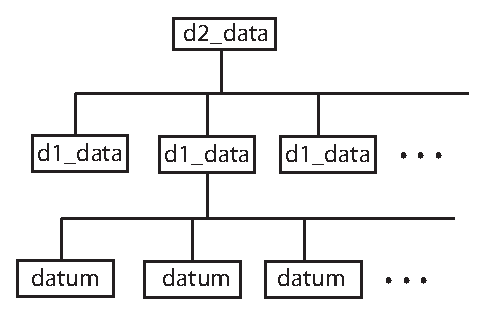
\includegraphics[width=4in]{data-tree.eps}
  \caption[Data tree structure]
{A \vn{d2\_data} structure holds a set of \vn{d1\_data} structures. 
A \vn{d1\_data} structure holds an array of datums.}
  \label{f:data.tree}
\end{figure}

\index{d2_data}\index{d1_data}\index{Data}
The horizontal orbit at a particular BPM is an example of an
individual \vn{datum}.  For ease of manipulation, arrays of datums are
grouped into what is called a \vn{d1_data} structure. Furthermore,
sets of \vn{d1_data} structures are grouped into what is called a
\vn{d2_data} structure.  This is illustrated in
Figure~\ref{f:data.tree}.  For example, a \vn{d2_data} structure for
orbit data could contain two \vn{d1_data} structures --- one
\vn{d1_data} structure for the horizontal orbit data and another
\vn{d1_data} structure for the vertical orbit data. Each datum of,
say, the horizontal orbit \vn{d1_data} structure would then correspond
to the horizontal orbit at some point in the machine.

When issuing \tao commands, all the
data associated with a \vn{d2_data} structure is specified using the
\vn{d2_data} structure's \vn{name}.  The data associated with a
\vn{d1_data} structure is specified using the format
\begin{example}
  d2_name.d1_name
\end{example}
For example, if a \vn{d2_data} structure has the
name ``\vn{orbit}'', and one of its \vn{d1_data} structures has the
name ``\vn{x}'', then \tao commands that refer to the data in this
\vn{d1_data} structure use the name ``\vn{orbit.x}''. Sometimes there
is only one \vn{d1_data} structure for a given \vn{d2_data}
structure. In this case the data can be referred to simply by using
the \vn{d2_data} structure's name. The individual datums can be
referred to using the notation
\begin{example}
  d2_name.d1_name[datum_index]
\end{example}
For example, \vn{orbit.x[10]} referrs to the horizontal orbit datum
with index 10. Notice that the beginning (lowest) datum index is user
selectable and is therefore not necessarily 1.

Ranges of datams can be referred to using using a comma \vn{,} to
separate the indexes combined with the notaion \vn{n1:n2} to specify
all the datums between \vn{n1} and \vn{n2} inclusive. For example
\begin{example}
  orbit.x[3:6,23]
\end{example}
refers to datums 3, 4, 5, 6, and 23. 

If multiple universes (\sref{s:universe}) are present, then the prefix
\vn{n@} signifies the n\Th universe. For example
\begin{example}
  2@orbit.x
\end{example}
would refer to the \vn{orbit.x} data in universe 2. When not
specified, the current ``viewed'' universe is assumed. The current
\vn{viewed} universe has index \vn{0} so \vn{orbit.x} is
equivalent to \vn{0@orbit.x}.

As explained in Section~\sref{s:data.anatomy}, each individual datum
has a number of components. The syntax to refer to a component is:
\begin{example}
  d2_name.d1_name[datum_index]|component
\end{example}
For example:
\begin{example}
  orbit.x[3:10]|meas     ! The measured data values
\end{example}

In referring to datums, a ``\vn{*}'' can be used as a wild card to 
denote ``all''. Thus:
\begin{example}
  *@orbit.x       ! The \vn{orbit.x} data in all universes.
  *               ! All the data in the currently viewed universe.
  *.*             ! Same as *
  *@*             ! All the data in all the universes. 
  *@*.*           ! Same as *@*
  orbit.x[*]|meas ! All measured values of orbit.x
  orbit.x|meas    ! Same as orbit.x[*]|meas
\end{example}
The last example shows that when referring to an entire block of data
encomposed by a \vn{d1_data} structure, the \vn{[*]} can be omitted.

%------------------------------------------------------------------------
\section{Anatomy of a Datum}
\label{s:data.anatomy}

Each datum has a number of quantities associated with it:
\begin{example}
  ele_name       ! Character: Corresponding lattice element name.
  ele0_name      ! Character: Name of range marker element.
  data_type      ! Character: Type of data: "orbit.x", etc.
  merit_type     ! Character: Type of constraint: 'target', 'max', etc.
  data_source    ! Character: How the datum is calculated. 'lattice', or 'beam'.
  ix_ele            ! Integer: Index of "ele" in the element list.
  ix_ele0           ! Integer: Index of "ele0" in the element list.
  ix_ele_merit      ! Integer: Lattice index where merit is evaluated.
  ix_d1             ! Integer: Index number in d1_data structure
  ix_data           ! Integer: Index in the global data array
  ix_dModel         ! Integer: Row number in the dModel_dVar derivative matrix.
  ix_bunch          ! Integer: Bunch number to get the data from.
  meas              ! Real: Measured datum value. 
  ref               ! Real: Measured datum value from the reference data set.
  model             ! Real: Datum value as calculated from the model.
  design            ! Real: What the datum value is in the design lattice.
  old               ! Real: The model at some previous time.
  base              ! Real: The value as calculated from the base model.
  fit               ! Real: The value as calculated from a fitting procedure.
  delta_merit       ! Real: Diff used to calculate the merit function term 
  weight            ! Real: Weight for the merit function term
  merit             ! Real: Merit function term value: weight * delta^2
  conversion_factor ! Real: Typically used to convert coupling to cbar
  s                 ! Real: longitudinal position of ele.
  relative          ! Logical: Is this a relative datum?
  exists            ! Logical: Does the datum exist?
  good_model        ! Logical: Does the model cmponent contain a valid value?
  good_meas         ! Logical: Does the meas cmponent contain a valid value?
  good_ref          ! Logical: Does the ref cmponent contain a valid value?
  good_user         ! Logical: Does the user want this datum used in optimization?
  good_opt          ! Logical: Can be used in Tao extensions.
  good_plot         ! Logical: Can be used in Tao extensions.
  useit_plot        ! Logical: Is this datum to be used in plotting?
  useit_opt         ! Logical: Is this datum to be used for optimization?
\end{example}
When running \tao, the \vn{show data}
(\sref{s:show}) command can be used to view the components of a datum. 
The \vn{set} command (\sref{s:set}) can be used to set some of these components.

%------------------------------------------------------------------------
\subsection{Datum values}
\label{s:datum.values}

\index{Data!measured}\index{Data!reference}\index{Data!model}
\index{Data!base}\index{Data!design}
A given datum has six values associated it:
\vspace{-2ex}
\begin{description}
  \vspace{-1ex}
  \item[meas] \Newline 
The value of the datum as obtained from some measurement. This is the
target or limit value that is used when running the optimizer. When
doing lattice design, the measured value corresponds to a constraint
value (\ref{c:opti}).
  \vspace{-1ex}
  \item[ref] \Newline
The reference datum value as obtained from some reference measurement. For example,
a measurement before some variable is varied could be designated as
the \vn{reference}, and the datum taken after the variation could be 
designated the \vn{measrued} datum.
  \vspace{-0.5ex}
  \item[model] \Newline
The value of the datum as calculated from the \vn{model} lattice (\sref{s:lattice}).
  \vspace{-0.5ex}
  \item[design] \Newline
The value of the datum as calculated from the \vn{design} lattice (\sref{s:lattice}).
  \vspace{-0.5ex}
  \item[base] \Newline
The datum value as calculated from the \vn{base} lattice (\sref{s:lattice}).
  \vspace{-0.5ex}
  \item[old] \Newline
A datum value that was saved at some point in \tao's calculations. This value
can be ignored.
\end{description}

%------------------------------------------------------------------------
\subsection{Associated Lattice Elements}
\label{s:datum.lat.elements}

\index{Data!Relative}
Associated with a datum are two lattice elements named
\vn{ele0_name} and \vn{ele_name}. Datums can be divided up into four
classes: Datums in the first class, like the emittance in a curcular
ring, do not have associated lattice elements and their corresponding
element names will be blank. Datums in the second class, like the beta
function at a given point, will only have one associated lattice
element given by \vn{ele_name} and \vn{ele0_name} will be blank.
Datums in the third class are associated with a section of the
lattice. For example, the maximum of the beta function in a lattice
region. In this case the \vn{ele0} element marks the beginning of the
region and \vn{ele} marks the end. The final class of datums, called
\vn{relative} datums, means that the datum value is set by the
difference between the value at the lattice element at \vn{ele0} and
the value at \vn{ele}. The betatron phase advance falls into this
category:
\begin{example}
  value = \(\phi\sb{x}\)(ele) - \(\phi\sb{x}\)(ele0)
\end{example}
If a relative datum has a blank \vn{ele0_name} then \vn{ele0} is taken
to be the beginning element of the lattice which is marker element
with index 0 named \vn{BEGINNING}.

The datum components \vn{ix_ele} and \vn{ix_ele0} are the index of
\vn{ele} and \vn{ele0} in the list of lattice elements.

%------------------------------------------------------------------------
\subsection{Datums in Optimization}
\label{s:datum.opt}

When using optimization to do lattice correction or design
(\sref{c:opti}), Individual datums can be excluded from the process
using the \vn{veto} (\sref{s:veto}), \vn{restore} (\sref{s:restore}),
and \vn{use} (\sref{s:use}) commands. These set the \vn{good_user}
component of a datum. This, combined with the setting \vn{exists},
\vn{good_model}, \vn{good_meas}, \vn{good_ref}, and \vn{good_opt}
determine the setting of \vn{useit_opt} which is the component that
determines if the datum is used in the computation of the merit
function. The settings of everything but \vn{good_user} is determined
by \tao

\vn{exists} is set by \tao to True if the datum exists and False
otherwise. A datum may not exist if the type of datum requires the
designation of an associated element but the \vn{ele_name} component
is blank. For example, a \vn{d1_data} array set up to hold orbit data
may use a numbering scheme that fits the lattice so that , say, datum
number 34 in the array does not correspond to an existing BPM.

\vn{good_model} is set according to whether a datum value can be
computed from the \vn{model} lattice. For example, If a circular
lattice is unstable, the beta function and the closed orbit cannot be
computed.

\vn{good_meas} is set True if the \vn{meas} component value is set in
the data initialization file (\sref{s:init.data}) or is set using the
\vn{set} command (\sref{s:set}). Similarly, \vn{good_ref} is set True
if the \vn{ref} component has been set. \vn{good_ref} only affects the
setting of \vn{useit_opt} if the optimization is using reference data
as set by the global variable \vn{opt_with_ref} (\sref{s:globals}).

Finally \vn{good_opt} is meant for use in custom versions of \tao
(\sref{c:custom.tao}) and is always left True by the standard \tao code.


%------------------------------------------------------------------------
\subsection{Datum Calculations}
\label{s:datum.calc}

Data can also be classified by how it is calculated:
\vspace{-2ex}
\begin{enumerate}
  \item \textbf{Lattice Parameters} \Newline
    For example lattice twiss parameters, coupling and floor position.
  \item \textbf{Single Particle Properties} \Newline
    For example particle orbit, BPM reading and phase advance.
  \item \textbf{Bunch Properties} \Newline
    For example bunch sigmas, emittance and beam twiss parameters.
\end{enumerate}
For a given data type the method used to calculate the datum can vary
depending on the tracking type. For {\it single} particle tracking all
data is found from the lattice parameters except for the orbit
data. For \textit{particle bunch} or \textit{macroparticle bunch}
tracking some of the datums are found from the particle distribution
using the appropriate \bmad routines. For example, with single
particle tracking the beta function is found from the lattice
transport matrix, however, with particle or macroparticle tracking the
beta function is found from the particle distribution using the
formula
\begin{equation}
  \beta_x = \frac{<x^{2}>}{\sqrt{<x^{2}> <x'^{2}> - <x x'>^{2}}}.
\end{equation}
The next section will describe how each predefined data type is
calculated.  Custom data types need not fall into one of the above
catagories and can be any real number as calculated in the appropriate
ook routine.


For datums with \vni{non-relative} \vn{data_types} if there is also an
associated \vni{ele0} element then the \vn{model} value is dependent
upon the \vni{merit_type}. For example, with a \vn{beta.x}
\vn{data_type} the model value is determined by Table~\ref{t:eval2}
where \vn{i} goes from the \vn{ele} index to the \vn{ele0} index.
\begin{table}[ht]
\centering
{\tt
\begin{tabular}{|l|l|l|} \hline
  {\it Merit\_Type}       & {\it Model Value} \\ \hline 
  \vni{abs_max} & $\min |\beta_x(i)|$ \\ \hline 
  \vni{abs_min} & $\min |\beta_x(i)|$ \\ \hline 
  \vni{int_max} &                     \\ \hline
  \vni{int_min} &                     \\ \hline
  \vni{min}     & $\min \beta_x(i)$ \\ \hline 
  \vni{max}     & $\min \beta_x(i)$ \\ \hline 
  \vni{target}  & {\it Error}   \\ \hline 
\end{tabular}
}
\caption{\vn{Model} evaluation.}
\label{t:eval2}
\end{table}

%------------------------------------------------------------------------
\section{Tao Data Types}\index{Data!Data Types}
\label{s:data.types}

Table~\ref{t:data.types} lists the predefined data types in \tao.

\vn{wire} data simulates the measurement of a wire scanner. The angle specified
is the angle of the wire with respect to the horizontal axis. The measurement
then measures the second momment $<uu>$ along an axis which is 90 degrees off of
the wire axis. For example, \vn{wire:90} is a wire scanner oriented in the
vertical direction and measures the second moment of the beam along the
horizontal axis, $<xx>$. The resultant data is not the beam size, but the beam
size squared.

Data types marked \vn{global} do not have any particular elements
associated with them.

Emittance can be calculated in one of two ways. One way is to
calculate it from a tracked beam. The other is from the lattice using
the standard radiation integrals (see the Bmad manual). For a linear
lattice, the emittance varies along the length of the line while for a
circular lattice there is a single emittance number. \vn{emit.a}
and \vn{emit.b} are the standard normal mode emittances. With
beam tracking, there are also \vn{projected emittances} which give an
indication of what the beam looks like if projected onto the $x$ or
$y$ axes:
\begin{equation}
  \eta_x (\mbox{(projected)} = \sqrt{<x^2> <p_x^2> - <x p_x>^2}
\end{equation}
Notice that this does {\emph not} correspond to the standard emittance
definition in one dimension:
\begin{equation}
  \eta_x = \sqrt{<(x - \eta_x \, p_z)^2> <(p_x - \eta'_x \, p_z)^2> - 
  <(x - \eta_x \, p_z) \, (p_x - \eta'_x \, p_z)>^2}
\end{equation}
\vn{emit.x} and \vn{emit.y} are the projected emittances.
Also notice that the projected emittance is sometimes defined using
$x'$ and $y'$ in place of $p_x$ and $p_y$. However, in the vast
majority of cases, this does not appreciably affect the numeric
results.

\index{Data!Calculation Method}
\index{unstable_ring}\index{beta}\index{alpha}\index{eta}\index{eta}
\index{etap}\index{phase}\index{orbit}\index{bpm}\index{wire}\index{spin}
\index{cbar}\index{coupling}\index{floor}\index{r}\index{t}\index{tt}
\index{i5a_e6}\index{i5b_e6}\index{s_position}\index{e_tot}
\index{unstable_ring}\index{emittance}\index{chrom}\index{norm_emittance}
\index{sigma}\index{dpx_dx}\index{dpy_dy}\index{dpz_dz}\index{dpa_da}
\index{dpb_db}
\begin{table}[ht] 
\centering 
{\tt\small
\begin{tabular}{|l|l|l|} \hline
  {\it Data\_Type}              & {\it Description}                  &          \\ \hline 
    alpha.x, alpha.y            & Projected Alpha Function           &          \\ \hline 
    alpha.a, alpha.b, alpha.z   & Normal-Mode Alpha Function         &          \\ \hline 
    e\_tot                      & Beam Total Energy                  &          \\ \hline
    beta.x, beta.y              & Projected Beta Function            &          \\ \hline 
    beta.a, beta.b, beta.z      & Normal-Mode Beta Function          &          \\ \hline 
    bpm.x, bpm.y                & Transverse BPM reading             &          \\ \hline 
    eta.x, eta.y                & Projected Dispersion               &          \\ \hline 
    eta.a, eta.b                & Normal-Mode Dispersion             &          \\ \hline 
    etap.x, etap.y              & Projected Dispersion derivative    &          \\ \hline 
    etap.a, etap.b              & Normal-Mode Dispersion derivative  &          \\ \hline 
    momentum\_compaction        & Momentum compaction factor         & relative \\ \hline
    orbit.x, orbit.y            & Transverse orbit                   &          \\ \hline 
    orbit.p\_x, orbit.p\_y      & Tranverse momenta                  &          \\ \hline 
    orbit.z, orbit.z\_p         & Longitudinal orbit and momenta     &          \\ \hline 
    phase.a, phase.b            & Betatron phase                     & relative \\ \hline 
    phase\_frac\_diff           & Fractional phase difference (x-y)  & relative \\ \hline
    \begin{tabular}{@{}l}     
      spin.polarization, \\ 
      spin.theta, spin.phi 
    \end{tabular} 
                          & Particle spin                      &          \\ \hline 
    \begin{tabular}{@{}l}     
      cbar.11, cbar.12, \\ 
      cbar.21, cbar.22 
    \end{tabular} 
                          & Coupling                          &          \\ \hline 
    \begin{tabular}{@{}l}   
      coupling.11b, coupling.12a, \\ 
      coupling.12b, coupling.22a 
    \end{tabular} 
                          & Coupling                          &          \\ \hline 
    floor.x, floor.y, floor.z
                          & Global (``floor'') position       & relative \\ \hline 
    floor.theta           & Global (``floor'') angle          & relative \\ \hline 
    r.$ij$                & 
                           \begin{tabular}{l}
                             Term in linear transfer map \\
                             $1 \le i,j \le 6$
                           \end{tabular}
                                                              & relative \\ \hline 
    t.$ijk$               & 
                           \begin{tabular}{l}
                             Term in 2\Nd order transfer map \\
                              $1 \le i,j,k \le 6$
                           \end{tabular} 
                                                              & relative \\ \hline 
    tt.$ijklm\ldots$      & 
                           \begin{tabular}{l}
                             Term in n\Th order transfer map \\
                              $1 \le i,j,k,\ldots \le 6$
                           \end{tabular} 
                                                              & relative \\ \hline 
    i5a\_e6, i5b\_e6      & Normalized I5 radiation integral  &          \\ \hline
    s\_position           & longitudinal length constraint    & relative \\ \hline 
    unstable\_ring        & Nonzero if a ring is unstable     & global   \\ \hline
    \begin{tabular}{@{}l}
      emit.x, emit.a \\
      emit.y, emit.b \\
      emit.z \\
    \end{tabular}
                          & Emittance                        & global   \\ \hline
    \begin{tabular}{@{}l}  
      norm\_emit.x, norm\_emit.a \\
      norm\_emit.y, norm\_emit.b \\
      norm\_emit.z \\
    \end{tabular} 
                          & Normalized Beam Emittance         &          \\ \hline 
    \begin{tabular}{@{}l}
      chrom.a, chrom.b  \\
    \end{tabular}
                          & Chromaticity for a ring           & global   \\ \hline
    \begin{tabular}{@{}l}   
      sigma.x, sigma.p\_x \\ 
      sigma.y, sigma.p\_y \\
      sigma.z, sigma.p\_z \\
    \end{tabular} 
                          & Bunch size                        &          \\ \hline 
    \begin{tabular}{@{}l}   
      multi\_turn\_orbit.x, multi\_turn\_orbit.p\_x \\ 
      multi\_turn\_orbit.y, multi\_turn\_orbit.p\_y \\
      multi\_turn\_orbit.z, multi\_turn\_orbit.p\_z \\
    \end{tabular} 
                          & Bunch size                        &          \\ \hline 
    \begin{tabular}{@{}l}  
      dpx\_dx, dpa\_da \\
      dpy\_dy, dpb\_db \\
      dpz\_dz \\
    \end{tabular} 
                          & <x p\_x> / <$x^2$> \& Etc...       &          \\ \hline 
    wire.<angle>                & Wire Scanner with wire angle <angle>
                                                               &          \\ \hline
\end{tabular}
} 
\label{t:data.types}
\caption{Predefined Data Types}
\end{table}

\vfill \break
{\vfill}



\chapter{Plotting}
\index{plotting}
\label{c:plotting}

\begin{figure}[b]
  \centering
  \includegraphics[width=4.5in]{plot-typical.pdf}
  \caption[An example of a plot display.]
{An example of a plot display. In this example there are three graphs: A graph displaying the beta
function, a graph displaying the orbit, and a graph displaying the ``lattice layout'' which shows
the longitudinal positions of lattice elements.}
  \label{f:plot.typ}
\end{figure}

\tao has a graphical display window within which such things as lattice functions, machine layout,
beam positions, etc., can be plotted. An example is shown in \fig{f:plot.typ} where there are plots
of the beta function and orbit along with a ``lattice layout which shows the longitudinal positions
of lattice elements. 

\tao organizes the display window using a number of concepts which are explained in the 
sections below
\begin{example}
  plot_page     ! The display window containing the graphics (\sref{s:plot.page.def}).
  regions       ! A set of rectangles on the plot_page that plots can be put in (\sref{s:region.def}).
  plot          ! A collection of graphs (\sref{s:plot.def}).
  box           ! Rectangular area within a plot that a graph is placed in (\sref{s:box.def}).
  graph         ! A diagram of some sort (\sref{s:graph.def}).
  curve         ! Data displayed within a \vn{graph} (\sref{s:curve.def}).
\end{example}

Underlying all this is the \vn{quick_plot} software toolkit (\sref{s:quick.plot}) which was developed
for \bmad and \tao for graphics plotting.

%-----------------------

\begin{figure}[bt]
  \centering
  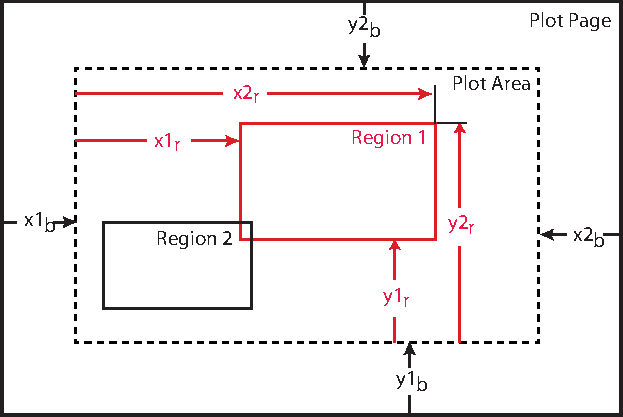
\includegraphics{plot-page.pdf}
  \caption[The plot window.]{The \vn{plot page} is the entire display window area. The \vn{plot area} 
is the region within the boarders of the \vn{plot page} within which ``\vn{regions}'' are
placed. The location of a \vn{region} is defined by four offsets with respect to the \vn{plot
area}. Regions may overlap.}
  \label{f:plot.page}
\end{figure}

%-----------------------------------------------------------------
\section{Plot Page}
\label{s:plot.page.def}

The \vn{plot page}, sometimes called the \vn{plot window}, refers to the window or the corresponding
printed graphics page where graphics are displayed. A \vn{plot page} is shown schematically in
\fig{f:plot.page}. Parameters associated with the \vn{plot page} are discussed in
\sref{s:plot.page}.  These parameters may be set in an initialization file or may be set on the \tao
command line using the \vn{set plot_page} (\sref{s:set.plot.page}) command. Examples:
\begin{example}
  set plot_page text_height = 11  ! 11 point font size
  set plot_page border%x1 = 0.2   ! Set left page border to 20% of width.
\end{example}

The size of the \vn{plot page} is set by the \vn{plot_page%size} parameter which is an array of two
numbers which set the width and height. The \vn{plot page} size can also be set when invoking \tao
using the \vn{-geometry} option (\sref{s:command.line})
\begin{example}
  > tao -lattice lat.bmad -geometry 300x500
\end{example}
This starts \tao with the \vn{plot page} size set to 300 points wide by 500 points high. It is also
sometimes convenient to start \tao without the plotting window. In this case, the \vn{-noplot} option
can be used on the startup command line. In a \tao initialization file, display of the plot window can be set
using the \vn{global%plot_on} parameter set in the \vn{tao_params} namelist (\sref{s:globals}).

In some cases, the screen resolution reported to \tao can be off. This has happened with some high
resolution displays where the reported resolution is 96 dpi when in fact the actual resolution is
much larger. In such a case, the size of the plot window created by \tao will be off. This can be
corrected by setting \vn{plot_page%size} appropriately but this in turn can create font size
problems. To avoid this problem, the environmental variable \vn{ACC_DPI_RESOLUTION} can be set to
the correct resolution before running \tao. The shell command line would be something like
\begin{example}
  > export ACC_DPI_RESOLUTION=168
\end{example}

The \vn{plot page} has a border within which \vn{regions} (\sref{s:region.def}) are defined. The area withing
the plot page border is called the \vn{plot area}

The \vn{show plot -page} (\sref{s:show.plot}) command may be used to view the page parameters.

%-----------------------------------------------------------------
\section{Region}
\label{s:region.def}

The \vn{plot area} is the area within the border of the \vn{plot page} as shown in
\fig{f:plot.page}.  In this \vn{plot area}, ``\vn{regions}'' can be defined which are invisible
rectangles where a \vn{plot} (\sref{s:plot.def}) can be placed. This is shown schematically in
\fig{f:plot.page}. Each region has a name and four numbers which specifies the location of the
region within the plot area. Regions may be defined by the user. In addition, for convenience, \tao
will define a number of regions. \tao defined regions will either begin with the letter ``\vn{r}''
or begin with the string ``\vn{layout}'' or the string ``\vn{scratch}''. Regions may overlap. How to
define regions is explained in \sref{s:plot.page}. The \vn{show plot} command will show the region
list. Example:
\begin{example}
  Tao> show plot

Plot Region         <-->  Plot                 x1    x2    y1    y2     Visible
-----------               -----------------------------------------------------
layout              <-->  lat_layout          0.00  1.00  0.00  0.15         T
r11                 <-->                      0.00  1.00  0.15  1.00
r12                 <-->                      0.00  1.00  0.58  1.00
r22                 <-->                      0.00  1.00  0.15  0.58
r13                 <-->  beta                0.00  1.00  0.72  1.00         T
r23                 <-->  dispersion          0.00  1.00  0.43  0.72         T
r33                 <-->  orbit               0.00  1.00  0.15  0.43         T
r14                 <-->                      0.00  1.00  0.79  1.00
\end{example}
The \vn{Plot} column shows what \vn{plot} (if any) is associated with the region
(\sref{s:plot.def}). The next four columns show the values of \vn{x1}, \vn{x2}, \vn{y1}, and \vn{y2}
set for the region. As shown in \Sref{s:plot.page}, \vn{x1} and \vn{x2} are the offsets from the
left \vn{plot area} edge to the left and right edges of the region. Similarly, \vn{y1} and \vn{y2}
are the offsets from the bottom edge of the \vn{plot area} to the bottom and top edges of the
region. \vn{x1} and \vn{x2} are normalized by the \vn{plot area} width and \vn{y1} and \vn{y2} are
normalized by the \vn{plot area} height so all four numbers should be in the range $[0, 1]$.  Using
the above example, the \vn{r23} region spans the full width of the \vn{plot area} (since \vn{x1} = 0
and \vn{x2} = 1), and occupies approximately the middle third vertically of the \vn{plot area}
(since \vn{y1} = 0.43 and \vn{y2} = 0.72).

The last column in the above shows if the \vn{plot} associated with the \vn{region} is
visible. Normally everything is visible. Invisibility is used in some special cases. For example,
when using a Graphical User Interface (GUI).

The \vn{set region} command can be used to set region parameters. Example:
\begin{example}
  set region r13 y1 = 0.8  ! Sets lower edge vertical position
\end{example}

%-----------------------------------------------------------------
\section{Plot}
\label{s:plot.def}

A \vn{plot} is essentially a collection of \vn{graphs}. This is shown schematically in
\fig{f:plot.plot} which shows a plot with two graph side by side.

Plots are divided into two groups. A \vn{template} plot defines how a \vn{displayed} plot is to be
constructed. That is, a \vn{template} plot defines what the associated \vn{graphs} are, defines
graph placement within the plot, etc. When a \vn{template} plot is \vn{placed} in a \vn{region},
either by using the \vn{place} command (\sref{s:place}) or by placement defined in an initialization
file (\sref{s:plot.page}), the information of the \vn{template} is copied in order to construct a
\vn{displayed} plot. A given \vn{template} plot may be placed in multiple \vn{regions} to give
multiple \vn{displayed} plots and then, using \vn{set} commands, the data displayed in each of these
plots may be manipulated separately. For example, one displayed orbit plot could show the orbit of
the \vn{model} lattice while another orbit plot could show the orbit difference between the
\vn{model} and \vn{design} lattices. When a \vn{plot} is displayed in a given \vn{region},
everything drawn is scaled to the region size.

Use the \vn{show plot} to see what displayed plots are associated with what regions. Use the
\vn{show plot -templates} command to see a list of \vn{template} plots. \tao defines a number of
default \vn{template} plots. Section~\sref{s:template} discusses how to define custom template
plots in an initialization file. Use the \vn{set plot} command (\sref{s:set.plot}) to modify either
\vn{template} or \vn{displayed} plots.

All plots have a name. A \vn{displayed} plot will inherit the same name of the \vn{template} plot it
came from. If a given \vn{template} plot is used to create multiple \vn{displayed} plots. All of
these plots will have the same name. A \vn{displayed} plot can also be referred to by using the
associated \vn{region} name. This can be used to remove ambiguity if there are multiple
\vn{displayed} plots of the same name. Additionally, a \vn{template} plot can unambiguously be
referred to by adding the prefix ``\vn{T::}'' to the plot name. Examples:
\begin{example}
  show plot           ! Show plots associated with regions
  show plot -template ! Show template plots
  place r13 orbit     ! Put orbit template into r13 region
\end{example}

Some commands, for example, the \vn{scale} command by default will ignore \vn{template} plots unless
the plot name has the \vn{T::} prefix. Other commands, for example the \vn{show plot} command, will
preferentially show displayed plot info but will show template plot info if there are no matching
displayed plots. Examples:
\begin{example}
  scale orbit -10 10    ! Scale all displayed orbit plots. Ignore template.
  scale r33 -10 10      ! Scale only plot in r33 region.
  scale T::orbit -10 10 ! Scale template orbit plot.
  show plot e_field     ! Will show displayed e_field plot info. If no
                        ! displayed plot exists, will show template info.
\end{example}

%-----------------------

\begin{figure}[bt]
  \centering
  \includegraphics[width=5.0in]{plot-plot.pdf}
  \caption[Plotting nomenclature.]
  {
A plot has a collection of graphs and a graph has a collection of curves. A graph is located within
a plot by defining the ``\vn{box}'' associated with the \vn{graph}. Illustrated here is a plot with
two graphs placed side by side.
  }
  \label{f:plot.plot}
\end{figure}

%-----------------------------------------------------------------
\section{Box}
\label{s:box.def}

To determine where a \vn{graph} is drawn with respect to the boundaries of its associated \vn{plot},
each \vn{graph} is associated with a given ``\vn{box}''. A \vn{box} is a rectangular sub-region of
the \vn{plot}. Boxes are defined by dividing the \vn{plot} into a rectangular grid and then choosing
one of the grid rectangles to be the \vn{box} associated with the \vn{graph}. The is illustrated in
\fig{f:plot.plot} where \vn{Graph 1} is associated with the \vn{box} labeled ``\vn{1,1,2,1}'' and
\vn{Graph 2} is associated with the \vn{box} labeled \vn{2,1,2,1}.  The last two digits of a
\vn{box} label (\vn{2,1} for both graphs) specify the number of rectangles the grid has horizontally
and vertically (2 horizontally, 1 vertically here). The first two digits (\vn{1,1} for \vn{graph 1}
and \vn{2,1} for \vn{graph 2}) specify the particular rectangle associated with the \vn{box} with
\vn{1,1} designating the lower left rectangle. Different \vn{graphs} do not have to use the same
grid division to select a box from.

Setting the \vn{box} for a given \vn{graph} in a \tao initialization file is covered in \sref{s:template}.
The \vn{set graph} and \vn{show graph} commands can be used to set and show the box parameters. 
Examples:
\begin{example}
  set graph myplot.g1 box = 2 1 2 2  ! Set box of graph myplot.g1
  set graph myplot.g2 box = 1 1 1 2  ! Different graphs can use different grids
                                     !  for box selection
\end{example}

%-----------------------------------------------------------------
\section{Graph}
\label{s:graph.def}

%-----------------------------------------------------------------
\subsection{Overview}
\label{s:graph.overview}

A \vn{graph} is a diagram of some sort. Most \vn{graph}s consists of horizontal and vertical axes
along with one or more \vn{curve}s. \vn{Floor_plan} (\sref{s:floor.plan}) and \vn{lat_layout}
(\sref{s:lat.layout}) \vn{graphs}, on the other hand, shows the placement in space of the lattice
elements and do not have any associated \vn{curves}.

Every \vn{plot} has at least one \vn{graph}. How many \vn{graphs} are associated with a \vn{plot}
is a matter of convenience and different \vn{graphs} of a \vn{plot} may display different types of
information. For example, it would be possible to have a single \vn{plot} contain three \vn{graphs}
and look like what is shown in \fig{f:plot.typ}. In actuality, the figure was constructed using
three \vn{plots} each one containing one \vn{graph}.

How to define \vn{graphs} when defining \vn{template} plots is given in \sref{s:template}. The
\vn{show graph} command can be used to show graph parameters. The \vn{set graph} command can
be used to modify \vn{graph} parameters.

%-----------------------------------------------------------------
\subsection{Graph Name}
\label{s:graph.name}

All graphs have a name. For example, the graph of the standard \vn{orbit} plot is simply ``\vn{g}''.
\vn{Graphs} may be referred to using the syntax:
\begin{example}
  <plot>.<graph>
\end{example}
where \vn{<plot>} is the plot name (or the \vn{region} name associated with the \vn{plot}) and
\vn{<graph>} is the graph name. If the \vn{.<graph>} ending is omitted, all graphs of the named
\vn{plot}(s) are selected. Examples:
\begin{example}
  show graph beta   ! Show info of all graphs in all the displayed beta plots.
  show graph r13.g1 ! Show info on ``g1'' graph of region r13.
\end{example}

%-----------------------------------------------------------------
\subsection{Curve Legend of a Graph}
\label{s:curve.legend}

The \vn{curve legend} is the legend identifying what curves are associated with what perimeters. In
\fig{f:plot.typ} the top two graphs have a curve legend in the upper left hand corner of the graph.
By default, the \vn{data_type} of each curve will be used as the text for that
curve's line in the legend.  This default can be changed by setting a curve's \vn{curve%legend_tex}.
Parameters that affect the curve legend are:
\begin{example}
  plot_page%legend_text_scale        ! Also affects lat_layout and floor_plan text size.      
  plot_page%curve_legend_line_len    ! tao_plot_page namelist (\sref{s:plot.page})
  plot_page%curve_legend_text_offset ! tao_plot_page namelist (\sref{s:plot.page})
  curve(N)%legend_text               ! 
  graph%curve_legend_origin          
  graph%draw_curve_legend            
\end{example}
The curve legend is distinct from the \vn{text legend} (\sref{s:text.legend}).

%-----------------------------------------------------------------
\subsection{Text Legend}
\label{s:text.legend}

The \vn{text legend} is a legend that can be setup by either the user or by \tao itself.
\tao uses the text legend in conjunction with phase space plotting or histogram displays.
The \vn{text legend} is distinct from the \vn{curve legend}. Parameters that affect the text
legend are:
\begin{example}
  graph%text_legend(:)      ! Array of strings to print
  graph%text_legend_origin  ! Position of legend.
\end{example}

%-----------------------------------------------------------------
\subsection{Graph Types}
\label{s:graph.types}

\tao defines several kinds of graphs. The \vn{graph%type} in the \vn{tao_template_graph}
(\sref{s:template}) sets the type.
\begin{description}
%
\item["data"] \Newline
``Data'' plotting is the plotting of a dependent variable on the $y$-axis vs an independent variable
on the $x$-axis. Typically the independent variable will be the longitudinal position $s$-position
as in the upper two graphs in \fig{f:plot.typ}. Also see \Sref{s:draw.ap} for an example where beam
apertures are added to the graph.

A ``\vn{data slice}'' graph is plotting one data array on the $y$-axis versus another data array on
the $x$-axis (\sref{s:graph.data.slice}). Also see \vn{parametric plotting} (\sref{s:param.plot}).

With a \vn{parametric} plot both the $x$ and $y$ values of the points on a curve are dependent
upon an independent parameter (\sref{s:param.plot}). This is similar to a \vn{data slice} plot
(\sref{s:graph.data.slice}).
%
\item["dynamic_aperture"] \Newline
A \vn{dynamic aperture} graph (\sref{s:da.plot}) draws the results from a dynamic aperture
calculation (\sref{s:da.calc}).
%
\item["floor_plan"] \Newline
A \vn{floor plan} graph shows the physical layout of the machine (\sref{s:floor.plan}). A table maps
lattice elements to a shape that is drawn (\sref{s:shapes}). The user may override the default
mapping. Besides the lattice elements. the outline of the building or tunnel that the machine is in
can be drawn (\sref{s:building.wall}).
%
\item["histogram"] \Newline
Currently \vn{histograms} (\sref{s:histogram}) are limited to displaying phase space data.
%
\item["key_table"] \Newline
The \vn{key table} displays information about variables bound to keyboard keys \sref{s:key.bind}.
Key bindings are used in \vn{single mode}.
%
\item["lat_layout"] \Newline
A \vn{lattice layout} graph displays the lattice elements as a series of shapes as a function of the
longitudinal position $s$ (\sref{s:lat.layout}). The lowest graph in \fig{f:plot.typ} is an example
of a \vn{lattice layout}.  A table maps lattice elements to a shape that is drawn (\sref{s:shapes}).
The user may override the default mapping.
%
\item["phase_space"] \Newline
A \vn{phase space graph} (\sref{s:phase.space}) displays particle positions in phase space after
a beam of particles has been tracked (\sref{s:beam.init}).
%
\item["wave.0", "wave.a", "wave.b"] \Newline
Wave analysis plotting (\sref{c:wave}).
%
\end{description}

\begin{figure}[b]
  \centering
  \includegraphics[width=5.0in]{plot-axes.pdf}
  \caption[Plot axes.]
{A data graph has three axes called \vn{x} (bottom edge), \vn{y} (left edge), and \vn{y2} (right edge).}
  \label{f:plot.axes}
\end{figure}

%-----------------------------------------------------------------
\subsection{Graph Axes}
\label{s:axes}

Data graphs (\sref{s:graph.types}) have three axes as shown in \fig{f:plot.axes}. The bottom axis is
called \vn{x}, and the left and right axes are called \vn{y} and \vn{y2} respectively. The
\vn{qp_axis_struct} structure (\sref{s:qp.axis}) is used to store axis parameters which can be
accessed via the \vn{graph%x}, \vn{graph%y}, and \vn{graph%y2} components in the
\vn{tao_template_graph} namelist (\sref{s:template}) or by using the \vn{set graph} command
(\sref{s:set.graph}.

The \vn{scale} command (\sref{s:scale}) can be used to set the vertical axes. The \vn{x_scale}
(\sref{s:x.scale}) command can be used to set the horizontal axis.

Normally there is only one vertical scale for a graph and this is associated with the \vn{y}
axis. However, if any curve of a given graph has \vn{curve%use_y2} set to \vn{True} then the \vn{y2}
axis will have an independent second scale. In this case, the \vn{y2} axis numbers will be
drawn. Notice that simply giving the \vn{y2} axis a label does {\em not} make the \vn{y2} axis scale
independent of the \vn{y} axis scale.

The following \vn{tao_plot_page} namelist (\sref{s:plot.page}) parameters affect the drawing of the axes:
\begin{example}
  text_height = 12              ! In points. Scales the height of all text
  axis_number_text_scale = 0.9  ! Relative to text_height
  axis_label_text_scale = 1.0   ! Relative to text_height
\end{example}

%-----------------------------------------------------------------
\section{Curve}
\label{s:curve.def}

%-----------------------------------------------------------------
\subsection{Overview}
\label{s:curve.overview}

A \vn{curve} is a data set to be displayed within a \vn{graph}. For example, a \vn{curve} may be the
beta function of the \vn{model} lattice. \vn{Curves} have an associated set of points at which a
symbol can be drawn. A curve also can have an associated curved line that can be drawn. For example,
in \fig{f:plot.typ} only the line is drawn with the two curves of the beta plot while both symbols
and line are drawn for the two curves of the orbit plot (here the data points where symbols are
drawn are the orbit at the edges of the lattice elements).

Some \vn{graphs} do not have any associated curves. For example, a \vn{lat_layout} graph does not
have associated curves.

How to define \vn{curves} when defining \vn{template} plots is given in \sref{s:template}. The
\vn{show curve} command can be used to show curve parameters. The \vn{set curve} command can
be used to modify \vn{curve} parameters.

%-----------------------------------------------------------------
\subsection{Curve Name}
\label{s:curve.name}

All curves have a name. \vn{Curves} may be referred to using the syntax:
\begin{example}
  <plot>.<graph>.<curve>
\end{example}
where \vn{<plot>} is the plot (or \vn{region}) name, \vn{<graph>} is the graph name and \vn{<curve>}
is the curve name. If the \vn{.<curve>} ending is omitted, all curves of the named \vn{graph}(s) are
selected. If the \vn{.<graph>.<curve>} ending is omitted, all curves of the named \vn{plot}(s) are
selected. Examples:
\begin{example}
  show curve beta   ! Show info of all curves in all the displayed beta plots.
  show curve r13.g1 ! Show info on curves in ``g1'' graph of region r13.
  set graph orbit.g curve_legend_origin = 0.1 -0.2 "%BOX/LT"  ! Set curve legend origin
\end{example}
The last example sets the \vn{curve legend} (\sref{s:template}) of the graph so that the curve
legend of the graph is drawn with respect to the left top corner of the box.

%-----------------------------------------------------------------
\subsection{Curve Line}
\label{s:curve.line}

Each curve may have an associated line that is drawn. The line may be a set of line segments
connecting curve symbol points (\sref{s:curve.sym}) or may be a ``smooth'' curve calculated by
evaluating the curve at a number of points. 

\vn{curve%draw_line} determines whether a curve is drawn through the data point symbols. The
thickness, style (solid, dashed, etc.), and color of the line can be controlled by setting
\vn{curve%line}. If \vn{plot%x_axis_type} is \vn{"s"}, and \vn{curve%component} does not contain
\vn{"meas"} or \vn{"ref"}, \tao will attempt to calculate intermediate values in order to draw a
smooth, accurate curve is drawn. Occasionally, this process is too slow or not desired for other
reasons so setting \vn{curve%smooth_line_calc} to False will prevent this calculation and the curve
will be drawn as a series of lines connecting the symbol points. The default of
\vn{curve%smooth_line_calc} is True. Use the \vn{set curve} command (\sref{s:set}) to toggle the
drawing of lines. Alternatively, the \vn{-disable_smooth_line_calc} switch can be used on the
command line (\sref{s:command.line}) or the global variable \vn{global%disable_smooth_line_calc} can
be set in the \tao initialization file (\sref{s:globals}).

The number of points to evaluate at when constructing a smoothed line is set by
\vn{plot_page%n_curve_pts} in the \vn{tao_plot_page} namelist (\sref{s:plot.page}) or by using the
\vn{set plot_page} command (\sref{s:set.plot.page}). To override this value for a particular plot
the \vn{plot%n_curve_pts} parameter can be set in the \vn{tao_template_plot} namelist or using the
\vn{set plot} command (\sref{s:set.plot}). More evaluation points may give a more accurate curve at
the expense of computation time.

%-----------------------------------------------------------------
\subsection{Curve Symbol}
\label{s:curve.sym}

\vn{curve%draw_symbols} determines whether a symbol is drawn at the data points. The size, shape and
color of the symbols is determined by \vn{curve%symbol}. A given symbol point that is drawn has
three numbers attached to it: The $(x, y)$ position on the graph and an index number to help
identify it. The index number of a particular symbol is the index of the datum or variable
corresponding the symbol in the \vn{d1_data} or \vn{v1_var} array. These three numbers can be
printed using the \vn{show curve -symbol} command (\sref{s:show}).  \vn{curve%draw_symbol_index}
determines whether the index number is printed besides the symbol. Use the \vn{set curve} command
(\sref{s:set}) to toggle the drawing of symbols. The default value for \vn{curve%draw_symbol} is
False if \vn{plot%x_axis_type} is \vn{"s"}, \vn{"curve"}, \vn{"lat"}, or \vn{"var"} and True
otherwise. The default \vn{curve%draw_symbol_index} is always False.

The \vn{graph%draw_only_good_user_data_or_vars} logical determines whether datums
(\sref{s:init.data}) or variables (\sref{s:init.var}) with a \vn{good_user} component set to
\vn{False} are drawn. The default is to not draw them which means that data or variables not used in
an optimization are not drawn.

%-----------------------------------------------------------------
\subsection{Curve Component}
\label{s:curve.comp}

A ``\vn{data}'' graph (\sref{s:graph.types}) is used to draw lattice parameters such as orbits, or
\tao data (\sref{c:data}), or variable values such as quadrupole strengths. The data values will
depend upon where the data comes from. This is determined, in part, by the setting of the
\vn{component} parameter in the \vn{tao_template_graph} namelist (\sref{s:template}).  The
\vn{component} may be one of:
\index{model}\index{design}\index{base}\index{meas}\index{ref}
\begin{example}
  "model"             ! model values. Default.
  "design"            ! design values.
  "base"              ! Base values
  "meas"              ! data values.
  "ref"               ! reference data values.
  "beam_chamber_wall" ! Beam chamber wall
\end{example}
Additionally, \vn{component} may be set to plot a linear combination of the above. For
example:
\begin{example}
  &tao_template_graph
    curve(2)%component = "model - design"
    ...
\end{example}
This will plot the difference between the \vn{model} and \vn{design} values. 
The default value of \vn{%component} is \vn{"model"}.

%-----------------------------------------------------------------
\subsection{Curve Data Source}
\label{s:curve.source}

\index{data}\index{var}\index{calculation}
\index{curve!data_source}
The \vn{data_source} parameter of a curve is the type of information for the source of the data points.
\vn{data_source} must be one of:
\begin{example}
  "data"              ! A d1_data array is the source of the curve points.
  "var"               ! A v1_var array is the source of the curve points.
  "lat" (Default)     ! The curve points are computed directly from the lattice.
  "beam"              ! The curve points are computed from tracking a beam of particles.
  "multi_turn_orbit"  ! Computation is from multi-turn tracking. 
\end{example}
The default for \vn{data_source} is \vn{"lat"}. With \vn{data_source} set to "\vn{data}",
the values of the curve points come from the \vn{d1_data} array structure named by
the curve's \vn{data_type} parameter (\sref{s:curve.type}).

If \vn{data_source} is set to \vn{var}, the values of the curve points come from a \vn{v1_var}
array structure. If it is set to \vn{lat} the curve data points are calculated from the lattice
without regard to any data structures. \vn{data_source} can be set to \vn{beam} when tracking
beams of particles. In this case, the curve points are calculated from the tracking. With \vn{beam},
the particular bunch that the data is extracted from can be specified via \vn{ix_bunch}. The
default is \vn{0} which combines all the bunches of the beam for the calculation.

Used in conjunction with \vn{data_type} and \vn{component} (\sref{s:curve.comp}). For
example (\sref{s:curve.source}), a curve of the orbit with \vn{data_source} set to \vn{"beam"}
would use the beam centroid computations. If the \vn{data_source} was set to \vn{"lat"} the
computed orbit using single particle tracking is used.

Example: With \vn{data_type} set to \vn{beta.x}, the setting of \vn{data_source} to
\vn{lat} gives the beta as calculated from the lattice and \vn{beam} gives the beta as calculated
from the shape of the beam.

%-----------------------------------------------------------------
\subsection{Curve Data Type}
\label{s:curve.type}

The \vn{data_type} of a curve specifies what is being plotted. What the valid settings for \vn{data_type}
are depends upon the type of graph (\sref{s:graph.types}). 
\begin{description}
%
\item[graph\%type = "data", or "histogram"] \Newline
Valid settings for \vn{data_type} are any \tao datum type (\sref{s:data.table}), \tao variable
(\sref{c:var}), and the following electric and magnetic field components:
\begin{example}
  b0_field.x,  b0_field.y,  b0_field.z,  b0_curl.x,  b0_curl.y,  b0_curl.z,  b0_div
  e0_field.x,  e0_field.y,  e0_field.z,  e0_curl.x,  e0_curl.y,  e0_curl.z,  e0_div
\end{example}
The field data types with names starting with ``b_'' and ``e_'' evaluate the field along the single
particle trajectory while the field data types with names starting with ``b0_'' and ``e0_'' are evaluated
along a constant transverse position specified by the curve's \vn{orbit} parameter.
%
\item[graph\%type = "dynamic_aperture"] \Newline
Valid settings for \vn{data_type} are:
\begin{example}
  "beam_ellipse"
  "dynamic_aperture"
\end{example}
%
\item[graph\%type = floor_plan", "lat_layout", or "key_table"] \Newline
There are not curves associated with these graph types.
%
\item[graph\%type = "phase_space"] \Newline
Valid settings for \vn{data_type} are:
\begin{example}
  "x",  "px",  "y",  "py",  "z",  "pz",
  "intensity",  "intensity_x",  "intensity_y"     ! Photon intensity
  "phase_x", "phase_y"                            ! Photon coherent phase
\end{example}
%
\end{description}

 For example, with \vn{graph%type} set to
\vn{dynamic_aperture} the 




Thus in the above example the curve point values are obtained from
\vn{orbit.x} data. To be valid the data structure named by \vn{data_type} must be set up in an
initialization file. If not given, the default \vn{data_type} is
\begin{example}
  <plot%name>.<graph%name>
\end{example}

%-----------------------------------------------------------------
\section{Quick_Plot Plotting}
\label{s:quick.plot}

\vn{Quick_plot} is a software library developed for \bmad and \tao for graphics plotting.

%-----------------------------------------------------------------
\subsection{Length and Position Units}
\label{s:qp.units}

Positions and lengths with \vn{quick_plot} generally have an associated ``\vn{units}'' string which determines how
$(x, y)$ positions or $(dx, dy)$ lengths are to be interpreted. 
The syntax of the \vn{units} parameter is:
\begin{example}
  "unit_type/ref_object/corner"
\end{example}
A \vn{units} string has a \vn{unit_type}, \vn{ref_object} and \vn{corner} components separated by slashes ``/''.

The \vn{unit_type} component is the type of units which can be one of:
\begin{example}
   "%"       - Percent.
   "DATA"    - Data units associated with a graph.
   "MM"      - millimeters.
   "INCH"    - Inches.
   "POINTS"  - Printers points (72 points = 1 inch, 1 pt ~ 1 pixel).
\end{example}
Note: If \vn{unit_type} is set to \vn{"DATA"}, \vn{ref_object}, if present, must be \vn{"GRAPH"} and
\vn{corner}, if present, must be \vn{"LB"}.

The \vn{ref_object} component is a reference object which can be one of:
\begin{example}
   "PAGE"  -- Relative to the plot display window.
   "BOX"   -- Relative to the box the graph is associated with.
   "GRAPH" -- Relative to the graph rectangle.
\end{example}
The \vn{ref_object} component is optional if a relative length is being specified and the
\vn{unit_type} is anything other than \vn, the slash between
the \vn{unit_type} and the \vn{ref_object} may be omitted.

Note: The \vn{"PAGE"} reference is the entire \vn{plot page} and not the \vn{plot area}. The
\vn{plot area} is only used for defining the placement of \vn{regions}.

The \vn{corner} component is the origin location of the reference object.
\vn{corner} can be one of:
\begin{example}
   "LB" -- Left Bottom of reference object. Default.
   "LT" -- Left Top.
   "RB" -- Right Bottom.
   "RT" -- Right Top.
\end{example}
The \vn{ref_object} component is optional if a relative length is being specified.

Examples:
\begin{example}
  "DATA"          -- Equivalent to "DATA/GRAPH/LB"
  "DATA/GRAPH/LB" -- Same as above.
  "DATA/BOX/RT"   -- ILLEGAL: DATA must always go with GRAPH/LB.
  "%/PAGE/LT"     -- Equivalent to "%PAGE/LT"
  "%PAGE/LT"      -- Percentage of page so (0.0, 1.0) = RT of page.
  "%BOX"          -- Percentage of box so (1.0, 1.0) = RT of box.
  "INCH/PAGE"     -- Inches from LB of page. Equivalent to "INCH/PAGE/LB"
\end{example}

Units can be set in an initialization file or with the \vn{set} command. Example:
\begin{example}
  set plot_page title%units = '%PAGE'
\end{example}

%-----------------------------------------------------------------
\subsection{Text Justification Units}
\label{s:qp.str.just}

Text justification units is a two character string that sets where a line of text is to be printed
with respect to the text $(x, y)$ position.
The first character of the justification string gives the horizontal alignment:
\begin{example}
   "L" -- Left justify
   "C" -- Center justify
   "R" -- Right justify
\end{example}
The second character of the justification string gives the vertical alignment:
\begin{example}
   "B" -- Bottom justify
   "C" -- Center justify
   "T" -- Top justify
\end{example}

Example:
\begin{example}
  plot_page%title%justify = 'CC'
\end{example}

%-----------------------------------------------------------------
\subsection{qp_point_struct}
\label{s:qp.point}

\vn{QuickPlot} defines a number of structures to parameterize such things like line and symbol
properties.

The \vn{qp_point_struct} defines where a point is:
\begin{example}
  type qp_point_struct:
    x     = <real>     ! Horizontal offset of point from fiducial point
    y     = <real>     ! Vertical offset of point from fiducial point
    units = "<units>"  ! Units of x \& y (\sref{s:qp.units}).
\end{example}
Example:
\begin{example}
  graph%curve_legend_origin = 5.0, -2.0, "POINTS/GRAPH/LT"
\end{example}
In this example the fiducial point the left-top point on the graph rectangle. The
\vn{curve_legend_origin} is positioned 5.0 points horizontally to the left and 2.0 points vertically
downward from this fiducial point.

%-----------------------------------------------------------------
\subsection{qp_line_struct}
\label{s:qp.line}

The parameters associated with data lines drawn in a graph are contained in the \vn{qp_line_struct}:
\begin{example}
  type qp_line_struct:
    width    = <integer>  ! Default = 1
    color    = <string>   ! Default = "black" (\sref{s:qp.color}).
    pattern  = <string>   ! Default = "solid" (\sref{s:qp.line.pat}).
\end{example}

%-----------------------------------------------------------------
\subsection{Symbols}
\label{s:qp.sym}

The parameters associated with symbols that are drawn are contained in the \vn{qp_symbol_struct}:
\begin{example}
  type qp_symbol_struct:
    type          = <string>  ! Default = "dot"
    height        = <real>    ! Size in points. Default = 10
    color         = <string>  ! Default = "black" (\sref{s:qp.color})
    fill_pattern  = <string>  ! Default = "solid_fill"
    line_width    = <integer> ! Default = 1.
\end{example}

\begin{table}
  \centering
  \includegraphics[width=5in]{plot-syms.pdf}
  \caption{Plotting Symbols.}
  \label{t:plot.syms}
\end{table}

The symbol types are:
\begin{example}
  square                 triangle                    square_concave              
  dot                    circle_plus                 diamond                     
  plus                   circle_dot                  star5                       
  times                  square_filled               triangle_filled           
  circle                 circle_filled               red_cross                 
  x                      star5_filled                star_of_david             
\end{example}
These symbols are illustrated in Table~\ref{t:plot.syms}. Symbol type names are case insensitive.

%-----------------------------------------------------------------
\subsection{qp_axis_struct}
\label{s:qp.axis}

The \vn{qp_axis_struct} structure defines the properties of a graph axis
\begin{example}
  type qp_axis_struct::
    label             = "<string>" ! Axis label string.
    min               = <real>     ! Min is the left or bottom axis number.
    max               = <real>     ! Max is the right or top axis number.
    number_offset     = <real>     ! Offset from axis line in inches.
    label_offset      = <real>     ! Offset from numbers in inches.
    major_tick_len    = <real>     ! Major tick length in inches.
    minor_tick_len    = <real>     ! Minor tick length in inches.
    label_color       = <string>   ! Color of the label string (\sref{s:qp.color})
    major_div         = <integer>  ! Number of major divisions
    major_div_nominal = <integer>  ! Major divisions nominal value.
    minor_div         = <integer>  ! Minor divisions. 0 = Tao will choose.
    minor_div_max     = <integer>  ! Max minor div number if Tao chooses.
    places            = <integer>  ! Number of digits to print
    type              = <string>   ! Axis type: "LINEAR" or "LOG".
    bounds            = <string>   ! Axis bounds: "GENERAL", "ZERO_AT_END", etc.
    tick_side         = <integer>  ! 1 = draw to the inside, 0 = both, -1 = outside.
    number_side       = <integer>  ! 1 = draw to the inside, -1 = outside.
    draw_label        = <logical>  ! Draw the label string
    draw_numbers      = <logical>  ! Draw the numbers.
\end{example}

The \vn{%bounds} parameter sets how the axes min and max values are calculated when plots are initially
instantiated and when \vn{scale}, \vn{x_scale}, and \vn{xy_scale} commands are used. Possible settings
are:
\begin{example}
  "ZERO_AT_END"      ! Min or max value is set to zero.
  "ZERO_SYMMETRIC"   ! Min and max chosen so that max = -min.
  "GENERAL"          ! No restrictions (default).
  "EXACT"            ! The User min/max is used.
\end{example}
If input min and max values are specified by the User, \tao will take the specified values as the starting
point to find ``nice'' min and max values to use. For example, with the command
\begin{example}
  scale all 0 19
\end{example}
and with \vn{bounds} set to \vn{"GENERAL"}, the min and max values will be set to 0 and 20. The exception is when
\vn{bounds} is set to \vn{"EXACT"}. In this case the User supplied min and max values will be used as is.

Examples:
\begin{example}
Tao> set graph r13 y%bounds = "zero_at_end"
Tao> scale r13 200 280   ! Graph bounds set to [0, 300]

Tao> set graph r13 y%bounds = "zero_symmetric"
Tao> scale r13 200 280   ! Graph bounds set to [-300, 300]

Tao> set graph r13 y%bounds = "general"
Tao> scale r13 20 190    ! Graph bounds set to [0, 200]

Tao> set graph r13 y2%bounds = "exact"
Tao> scale r13 -y2 20 190    ! Y2 graph bounds set to [20, 190]
\end{example}

Both \vn{major_div} and \vn{major_div_nominal} set the number of major divisions in the plot. The
difference between the two is that with \vn{major_div} set positive and \vn{major_div_nominal} set
zero or negative, the number of major divisions is fixed at the value of \vn{major_div}. With
\vn{major_div_nominal} positive, the value of \vn{major_div} is ignored, and the number of major
divisions will be chosen to be a ``nice'' value near the value of \vn{major_div_nominal}. If neither
\vn{major_div} nor \vn{major_div_nominal} is set positive, a value will be chosen for
\vn{major_div_nominal} by \tao. If you are unsure which to set, it is recommended that
\vn{major_div_nominal} be used.

The \vn{places} parameter set the number of places to display a number. \tao will automatically
calculate this number and it is not user settable.

The \vn{label} parameter may include Greek letters, subscripts, superscripts, and special characters.
Encoding for these are given in Table~\ref{t:plot.escape}. 

%-----------------------------------------------------------------
\subsection{qp_legend_struct}
\label{s:qp.legend.str}

The parameters associated with drawing a curve legend (\sref{s:plot.def}) are contained in the parameter
\vn{plot_page%curve_legend} (\sref{s:plot.page}). This parameter is an instance of a \vn{qp_legend_struct}
which has the structure:
\begin{example}
  type qp_legend_struct
    type (qp_point_struct) origin  ! Location of legend.
    row_spacing = <real>           ! Spacing between rows. Default = 1.0.
    line_length = <real>           ! Length of the line in points.
    text_offset = <real>           ! Horizontal offset in points between the line and the text.
    logical draw_line = <logic>    ! Draw lines?
    logical draw_symbol = <logic>  ! Draw symbols?
    logical draw_text = <logic>    ! Draw text?
  end type
\end{example}

%-----------------------------------------------------------------
\subsection{String Escape Sequences}
\label{s:qp.str}

\begin{table}[tb]
\begin{tabular}{ll} \toprule
{\B}u       & Start a superscript or end a subscript \\[0.3ex]
{\B}d       & Start a subscript or end a superscript.
              {\B}u and {\B}d must always be used in pairs \\[0.3ex]
{\B}b       & Backspace (i.e., do not advance text pointer  
               after plotting the previous character) \\[0.3ex]
{\B}fn      & Switch to Normal font (1)       \\[0.3ex]
{\B}fr      & Switch to Roman font (2)        \\[0.3ex]
{\B}fi      & Switch to Italic font (3)       \\[0.3ex]
{\B}fs      & Switch to Script font (4)       \\[0.3ex]
{\B}{\B}    & Backslash character (\B)        \\[0.3ex]
{\B}x       & Multiplication sign ($\times$)  \\[0.3ex]
{\B}.       & Centered dot ($\cdot$)          \\[0.3ex]
{\B}A       & Angstrom symbol (\AA)         \\[0.3ex]
{\B}gx      & Greek letter corresponding to roman letter x. See Table~\ref{t:greek}. \\[0.3ex]
{\B}mN {\B}mNN & Graph marker number \vn{N} or \vn{NN} (1-31) \\[1ex]
{\B}(NNNN)  & 
\parbox{5.2in} {Character number NNNN (1 to 4 decimal digits) from the Hershey character set which
includes a number of special characters including mathematical, musical, astronomical, and
cartographical symbols.} \\ \bottomrule
\end{tabular}
\caption{Escape Sequences for Labels.}
\label{t:plot.escape}
\end{table}

Table~\ref{t:greek} shows how the character string \vn{"{\B}g<r>"}, where \vn{"<r>"} 
is a Roman letter, map onto the Greek character set.
\begin{table}[tb]
  \centering
  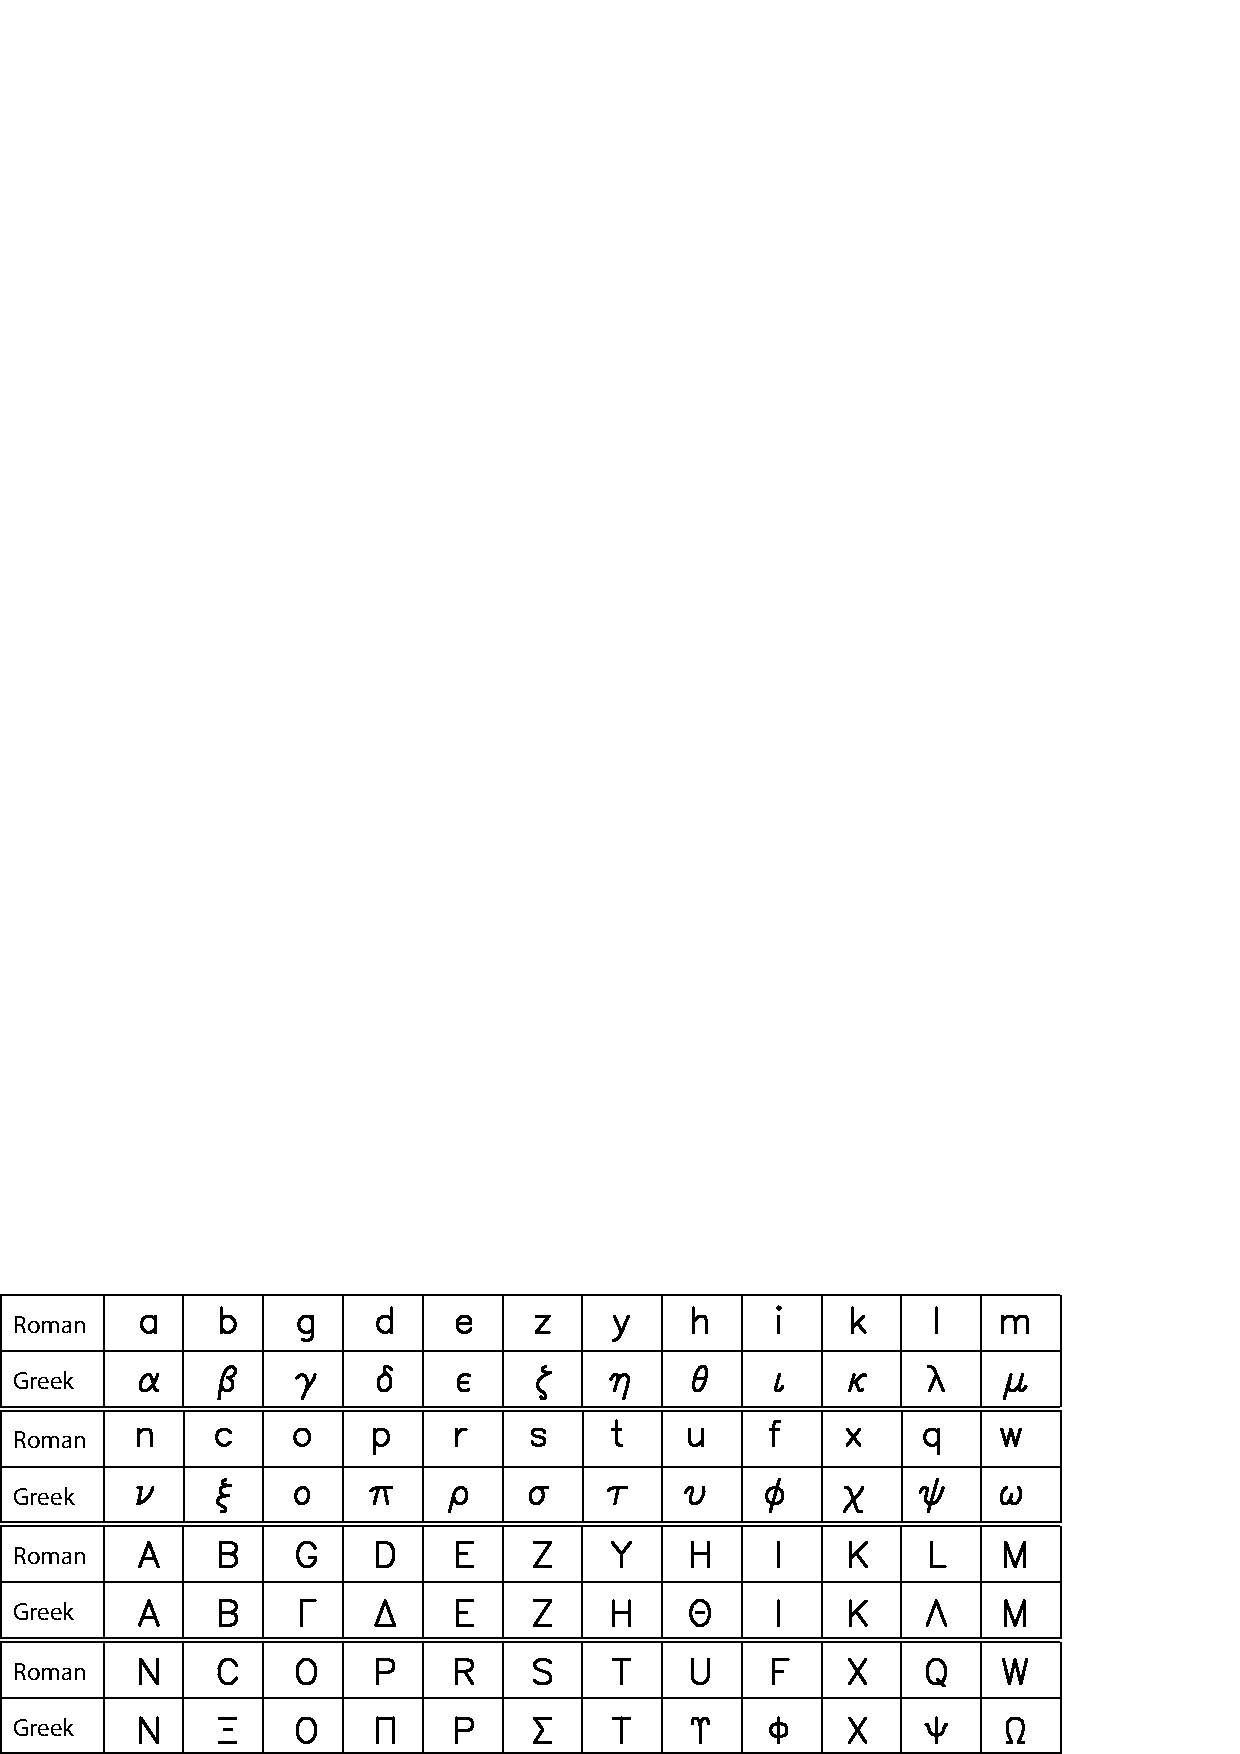
\includegraphics[width=5.0in]{greek.pdf}
  \caption[Roman to Greek Character Conversion]{Conversion for the string 
\vn{"{\B}g<r>"} where \vn{"<r>"} is a Roman character to the corresponding 
Greek character.}
\label{t:greek}
\end{table}

%-----------------------------------------------------------------
\subsection{Color Names}
\label{s:qp.color}

Possible settings for color parameters are:
\begin{example}
  White   (actually the background color)       Orange          
  Black   (actually the foreground color)       Yellow_Green    
  Red                                           Light_Green         
  Green                                         Navy_Blue       
  Blue                                          Purple          
  Cyan                                          Reddish_Purple  
  Magenta                                       Dark_Grey        
  Yellow                                        Light_Grey       
\end{example}
Color names are case insensitive.

%-----------------------------------------------------------------
\subsection{Line Pattern Names}
\label{s:qp.line.pat}

Possible settings for line patterns are:
\begin{example}
  solid      ! Solid line                 dotted     ! Dotted line             
  dashed     ! Dashed line                dash_dot3  ! Dash--dot--dot--dot line
  dash_dot   ! Dash--dot line
\end{example}
Pattern names are case insensitive.

%-----------------------------------------------------------------
\subsection{Fill Pattern Names}
\label{s:qp.fill.pat}

Possible fill pattern settings for symbols are:
\begin{example}
  solid_fill                    hatched           
  no_fill                       cross_hatched     
\end{example}
Fill pattern names are case insensitive.


\chapter{Optimization}
\label{c:opti}

%------------------------------------------------------------------------
\section{Lattice Corrections}

Examples of lattice corrections include flattening the orbit and
adjusting quadrupoles to correct the measured betatron phase. The
general idea is to vary an appropriate set of \vn{variables} with the
aim of minimizing a merit function \vn{M} that is a measure of how
well \vn{data_model}, the data as calculated from the \vn{model} fits
\vn{data_meas}, the measured data
\Begineq
  {\cal M} \equiv \sum_{i} w_i \,
    (\data\_\model(i) -  \data\_\meas(i))^2 + 
  \sum_{j} w_j \,
    (\var\_\model(j) - \var\_\meas(j))^2
  \label{m1}
\Endeq
\vn{var_model} is the value of a variable in the \vn{model} and
\vn{var_meas} is the value as measured at the time the data was taken
and the sum \vn{j} runs over all variables that are allowed to be
varied to minimize \vn{M}. The second term in the merit function
prevents degeneracies (or near degeneracies) in the problem which
would allow \tao to find solutions where \vn{data_model} matches
\vn{data_measured} with the \vn{var_model} having ``unphysical''
values (values far from \vn{var_meas}. The weights $w_i$ and $w_j$
need to be set depending upon how accurate the measred data is
relative to how accurate the calibrations for measuring the
\vn{var_meas} values are. With the second term in the merit function
the number of constraints (number of terms in the merit function) is
always larger than the number of variables and degeneracies can never
occur. 

The algorithm used to vary the \vn{var_model} variables to minimize
\vn{M} is called an \vn{optimizer}. In \vn{command line mode} the
\vn{run} command is used to invoke an \vn{optimizer}. In \vn{single
mode} the \vn{g} key starts an optimizer and the \vn{.} key stops it.
Running an optimizer is also called ``fitting'' since one is tring to
get the \vn{data_model} to be equal to the \vn{data_meas}. With orbits
this is also called ``flattening'' since one generally wants to end up
with an orbit that is on--axis.

In a correction one wants to change the machine variables so that the
measured data corresponds to the design values \vn{data_design}. Thus
the change in the data that one wants is
\begin{example}
  data_change = data_design - data_meas
\end{example}
Once a fit has been made, and presuming that the \vn{data_model} is
resonably close to the \vn{data_meas} this data change within the
\vn{model} lattice can be accomplished by changing the variables by
\begin{example}
  var_change = var_design - var_model
\end{example}
This assumes the system is linear. For many situations this is true
since typically \vn{var_change} is ``small''. Since the variables have
a measrued value of \vn{var_meas} the value that the variables should
be set to is
\begin{example}
  var_final = var_meas + (var_design - var_model)
\end{example}
Notice that the fitting process is independent of the \vn{design}
lattice. It is only when calculating the corrections to the
variables that the \vn{design} lattice plays a roll. 

Sometimes it is desired to fit to changes in data as opposed to the
absolute value of the data. For example, when closing an orbit bump
knob what is important is the difference in orbits before and after
the bump knob is varied. Designating one of these orbit the
\vn{reference}, the appropriate merit function is
\begin{alignat}{1}
  {\cal M} = &\sum_{i} w_i \,
    \left[ \bigl( \data\_\model(i) - \data\_\design(i) \bigr) - 
      \bigl( \data\_\meas(i) - \data\_\reference(i) \bigr) \right]^2 + \CRNO
  &\sum_{j} w_j \,
    \left[ \bigl( \var\_\model(j) - \var\_\design(j) \bigr) -
     \bigl( \var\_\meas(i) - \var\_\reference(i) \bigr) \right]^2 
  \label{m2}
\end{alignat}
where \vn{data_ref} and \vn{var_ref} refer to the reference
measurement.  This merit function is acceptable if the reference data
is taken with the machine reasonably near the design setup so that
nonlinearities can be ignored. If this is not the case then the
fitting becomes a two step process: The first step is to fit the
\vn{model} to the \vn{reference} data using the merit function of
\Eq{m1}. The \vn{base} lattice is then set equal to the \vn{model}
lattice. The second step is to fit the model using the merit function
\begin{alignat}{1}
  {\cal M} = &\sum_{\data: i} w_i 
    \left[ (\data\_\model(i) - \data\_\base(i)) - 
      (\data\_\meas(i) - \data\_\reference(i)) \right]^2 + \CRNO
  &\sum_{\var: j} w_j 
    \left[ (\var\_\model(j) - \var\_\base(j)) -
     (\var\_\meas(i) - \var\_\reference(i)) \right]^2 
  \label{m3}
\end{alignat}

Control of what data and what variables are to be used in the fitting
process is controlled by the \vn{use}, \vn{veto}, \vn{restore}, and
\vn{clip} commands.

%------------------------------------------------------------------------
\section{Lattice Design}

Lattice design is the process of calculating \vn{variable} strengths
to meet a number of criteria called constraints. For example, one
constraint could be that the beta function in some part of the lattice
not exceed a certain value. In this case we can proceed as was done
for lattice correction and define a merit function to be minimized:
\Begineq
  {\cal M} = \sum_{\mbox{constraints} i} w_i \, C_i^2
\Endeq
The general form of the $C_i$ constraint values is
\Begineq
  C = 
    \begin{cases}
    (\mbox{Model} - \mbox{Target})  & Condition \\
    0                               & Otherwise
    \end{cases}
\Endeq
where \vn{model} is the value as calculated from the \vn{model}
lattice and \vn{target} is some given number. Part of the optimization
process is in deciding what the values should be for the \vn{targets}.
The \vn{condition} needed for a non--zero $C_i$ is dependent upon the
\vn{type} of the constraint. There are five constraint types:
\begin{table}[h]
\centering
{\tt
\begin{tabular}{|l|l|l|} \hline
  {\it Constraint Type}  & $C$ & {\it Condition for non-zero $C$} \\ \hline 
  \vn{target}     & \vn{model} - \vn{target}   & \vn{model} $\ne$ \target     \\ \hline 
  \vn{min}        & \vn{model} - \vn{target}   & \vn{model} $<$ \vn{target}   \\ \hline 
  \vn{max}        & \vn{model} - \vn{target}   & \vn{model} $>$ \vn{target}   \\ \hline 
  \vn{abs_min}    & |\vn{model}| - \vn{target} & |\vn{model}| $<$ \vn{target} \\ \hline 
  \vn{abs_max}    & |\vn{model}| - \vn{target} & |\vn{model}| $>$ \vn{target} \\ \hline 
\end{tabular}
}
\caption{Constraint Type List.}
\label{t:con_type}
\end{table}

Since lattice design and lattice corrections are very similar, \tao
combines the two into one generalized correction process. With \tao
the constraint \vn{model} values are identified with the
\vn{data_model} and the \vn{target} values are identified with the \vn{data_meas}.
The different types of \vn{data} that \tao knows about is called the data's \vn{type}

\begin{table}[h] \centering {\tt
\begin{tabular}{|l|l|l|} \hline
  {\it Constraint/Data Type} & {\it Description}     &          \\ \hline 
    beta:x, beta:y    & Twiss parameter              &          \\ \hline 
    alpha:x, alpha:y  & Twiss parameter              &          \\ \hline 
    eta:x, eta:y      & Dispersion                   &          \\ \hline 
    etap:x, etap:y    & Dispersion derivative        &          \\ \hline 
    phase:x, phase:y  & Betatron phase               & relative \\ \hline 
    orbit:x, orbit:y  & Particle orbit               &          \\ \hline 
    cbar:11, cbar:12, cbar:21, cbar:22 
                      & Coupling                     &          \\ \hline 
    floor:x, floor:y, floor:z
                      & Global (``floor'') position  & relative \\ \hline 
    floor:theta       & Global (``floor'') angle     & relative \\ \hline 
    r56            & Term in linear transfer map     & relative \\ \hline 
    t566           & Term in 2nd order transfer map  & relative \\ \hline 
    s              & Longitudinal length constraint  & relative \\ \hline 
\end{tabular}
} \caption{Constraint List.}  \label{t:cons}
\end{table}

\chapter{Wave Analysis}
\label{c:wave}


%----------------------------------------------------------------
\section{General Description}
\label{s:wave.general}

A ``wave analysis'' is method for finding isolated ``kick errors'' in
a machine by analyzing the appropriate data. Types of data that can be
analyzed and the associated error type is shown in
Table~\ref{t:wave0}.  

The analysis works on difference quantities. For example, the
difference between measurement and theory or the difference between
two measurements. Orbit and vertical dispersion measurements are the
exception here since an analysis of, say, just an orbit mesurement can
be considered to be the difference between the measurement and a
perfectly flat (zero) orbit.

\begin{table}[h]
\centering{\tt
\begin{tabular{|l|l|} \hline
  {\it Measurement Type}  & {\it Error Type}           \\ \hline
  Orbit                   & Steering errors            \\ \hline
  Betatron phase          & Quadrupolar errors         \\ \hline
  Beta function           & Quadrupolar errors         \\ \hline
  Coupling                & Skew quadrupolar errors    \\ \hline
  Dispersion              & Sextupole errors           \\ \hline
\end{tabular}}
\caption[Wave measurement types.]
{Types of measurements that can be used in a wave analysis and the 
types of errors that can be diagnosed.}
\label{t:wave0}
\end{table}

The formulation of the wave analysis for quadrupolar and skew
quadrupolar errors is presented by Sagan\cite{b:wave}.  Although not
discussed in the paper, the wave analysis for orbit and dispersion
measurements is similar to the beta function analysis that is
presented. 

The wave analysis is similar for all the measurement types. How the
wave analysis works is illustrated in Figure~\ref{f:wave0}.
Figure~\ref{f:wave0}a shows a simulated orbit for the Cesr Storage
Ring. The horizontal axis is the detector index. In this example, the
orbit represents the effect of two kicks generated by steerings near
detector 40 and detector 80.

For the wave analysis, two regions of the machine, labeled $A$ and $B$
in the figure, are chosen (more on this later). For each region in
turn, the data in that region is fit using a functional form that
assumes that there are no kick errors in the regions. For orbits, this
functional form is the standard equation
\Begineq
  x(s) = A \, \sqrt{\beta(s)} \, \sin(\phi(s) \, s + phi_0)
  \label{xabps}
\Endeq
where $\beta$ is the beta function and $\phi$ is the phase
advance. The quantities $A$ and $\phi_0$ are varied to give the best
fit.  Once $A$ and $\phi_0$ are fixed, \Eq{xabps} can be evaluated at
any point. Figure~\ref{f:wave0}b shows the orbit of \ref{f:wave0}a
with the fit to the $A$ region subtracted off. Similarly,
Figure~\ref{f:wave0}c shows the orbit of Figure~\ref{f:wave0}a with
the fit to the $B$ region subtracted off. Concentrating on
Figure~\ref{f:wave0}b, since there are no kick errors in the $A$
region, the fit is perfect and hence the difference between the data
and the fit is zero. Moving to the right from the $A$ region in
Figure~\ref{f:wave0}b, this difference is zero up to where the
assumption of no kick errors is violated. That is, at the location of
the kicker near detector 40. Similarly, since there are no kick errors
in region $B$, the difference between the data and the $B$ region fit
is zero in Figure~\ref{f:wave0}c and this remains true moving leftward
from region $B$ up to the kicker near detector 40.

By taking the fitted values for $A$ and $\phi_0$ for the regions $A$
and $B$, the point between the regions where the kick is generated and
the amplitude of the kick can be calculated. This calculation is
similar to that used to find quadrupolar errors from beta
data\cite{f:wave0}. The one difference is a factor of 2 that appears
in the beta calculation due to the fact that a freely propagating beta
wave oscillates at $2\phi(s)$. 

The success of the wave analysis in finding a kick error depends upon
whether there are regions of sufficient size on both sides of the kick
that are kick error free. That is, whether the kick error is
``isolated''. The locations of the $A$ and $B$ regions are set by the
user and the general strategy is to try to find, by varying the
location of the regions, locations where the data is well fit within
the regions. The data is well fit if the difference between data and
fit is small compared to the data itself. If there are multiple
isolated kick errors, then each error in turn can be bracketed and
analyzed. If there are multiple errors so close together that they
cannot be resolved, this will throw off the analysis, but it may still
be possible to give bounds for the location where the kicks are at and
an ``effective'' kick amplitude can be calculated.

For circular machines, to be able to analyze kicks near the beginning
or end of the lattice, the wave analysis can be done by ``wrapping''
the data past the end of the lattice for another 1/2 turn. This is
illustrated in Figure~\ref{f:wave0}. In the Cesr machine, there are
approximately 100 detectors labeled from 0 to 99.  The detectors from
100 to 150 are just the detectors from 0 to 50 shifted by 100. Thus,
for example, the detector labeled 132 in the figure is actually
detector 32.

%----------------------------------------------------------------
\section{Wave Analysis in Tao}
\label{s:wave.tao}

Proforming a wave analysis in \tao is a three step process:
\begin{example}
  1) Plot the data to be analyzed.
  2) Use the \vn{wave} command to select the data.
  3) Use the \vn{set wave} command to vary the fit regions.
\end{example}

In general, the accuracy of the wave analysis depends upon the
accuracy with which the beta function and phase advances are known in
the baseline lattice used. \tao uses the \vn{model} lattice for the
baseline. If possible, One strategy to improve the accuracy of the
wave analysis is first use a measurement to calculate what the
quadrupole strengths in the \vn{model} lattice should be. Possible
measurements that can give this information include an orbit response
matrix (ORM) analysis, fits to beta or betatron phase measurements, etc.

%----------------------------------------------------------------
\subsection{Prepairing the Data} 
\label{ss:wave.data}

At present (due to limited manpower to do the
coding), the wave analysis is restricted to data that is stored in a
d1_data array (\sref{c:data}). That is, the plotted curve to be
analyzed must have its \vn{data_type} parameter set to
\vn{'data_array'} (\sref{s:init.data}). The possible data types that
can be analyzed are:
\begin{example}
  orbit.x, orbit.y
  beta.a,  beta.b
  phase.a, phase.b
  eta.x, eta.y
  cbar.12
\end{example}
The curve to be analyzed must be visible. Any combination of data
components may be used:. "meas", "meas-ref", "model", etc.

If data from a circular machine is being analyzed, the data is wrapped
past the end of the lattice for another 1/2 turn. The translation from
the data index in the wrapped section to the first 1/2 section of the
lattice is determined by the values of \vn{ix_min_data} and
\vn{ix_max_data} of the d1_data array under consideration
(\sref{s:init.data}):
\begin{example}
  index_wrap \longrightarrow index_wrap - (ix_max_data - ix_min_data + 1)
\end{example}
For example, for the Cesr example in the previous section,
\vn{ix_min_data} was 0 and \vn{ix_max_data} was 99 to the translation
was
\begin{example}
  index_wrap \longringtarrow index_wrap - 100
\end{example}

%----------------------------------------------------------------
\subsection{Wave Analysis Commands}
\label{ss:wave.cmd}

The \vn{wave} command (\sref{s:wave}) sets which plotted data curve
is used for the wave analysis. The \vn{set wave} command (\sref{s:set}) 
is used for setting the $A$ and $B$ region locations. Finally the 
\vn{show wave} command (\sref{s:show}) prints analysis results. 

%----------------------------------------------------------------
\subsection{The Wave Analysis Output}
\label{ss:wave.cmd}


\chapter{Tao Initialization}\index{Initialization}
\label{c:init}

\tao is customized for specific machines and specific calculations
using input files and custom software routines. Writing custom
software is covered in the programmer's guide section. This chapter
covers the input files.

In general, the input files tell \tao:
\begin{example}
  1) What the "standard" variables should be.
  2) What the "standard" data is.
  3) What to plot and where to plot it.
\end{example}

\tao first looks for input files in the current directory and then
looks in a directory pointed to by the environmental variable
\vn{TAO_INIT_DIR}.

Initialization parameters are read in from a file using Fortran
namelist input. Fortran namelist breaks up the input file into
blocks. The first line of a namelist block starts with an ampersand
``\&'' followed by the block identifying name. Variables are assigned
using an equal sign ``='' and the end of the block is denoted by a
slash ``/'' For example:
\begin{example}
  &this_block_name
    var1 = 0.123   ! exclamation marks are used for comments
    var2 = 0.456
  /
\end{example}
Variables that have default values can be omitted from the block.  The
order of the variables inside a block is irrelevant.  In between
namelist blocks all text is ignored. Inside a block comments may be
included by using an exclamation mark ``!''.

Note: string variables are case sensitive.

%-----------------------------------------------------------------
\section{Beginning Initialization}
\index{Initialization!beginning}
\label{s:init_global} 


\index{tao_start}
\index{tao.init}
\index{lattice_file}
\index{data_file}
\index{var_file}
\index{plot_file}
\index{single_mode_file}
\index{startup_file}
\index{n_universes}
\index{startup_single_mode}
The initialization starts with an initialization file named
\vn{tao.init}.  \vn{tao.init} needs to have a \vn{tao_start} namelist
block with the following syntax:
\begin{example}
  &tao_start
    lattice_file      = "<file_name>"  ! Default = this file.
    data_file         = "<file_name>"  ! Default = this file.
    var_file          = "<file_name>"  ! Default = this file.
    plot_file         = "<file_name>"  ! Default = this file.
    single_mode_file  = "<file_name>"  ! Default = this file.
    startup_file      = "<file_name>"  ! Default = "tao.startup"
    n_universes       = <integer>            ! Number of universes. Default = 1.
    init_name      = "<init_name>" !Default = 'Tao"
  /
\end{example}
\vn{n_universes} is the number of universes to be created.  \vn{init_name} is
for naming the initialization. This is useful to distinguish between multiple
initialization files with custom versions of \tao.  The other parameters specify
which files to find the other initialization namelists. The following sections
describe each of these initialization namelists and their locations are listed
in table \ref{t:init_files}.

\index{tao_design_lattice}
\index{tao_params}
\index{tao_coupled_uni_init}
\index{tao_beam_init}
\index{tao_macro_init}
\index{tao_var}
\index{tao_d2_data}
\index{tao_d1_data}
\index{tao_plot_page}
\index{tao_template_plot}
\index{tao_template_graph}
\index{element_shapes}
\index{key_bindings}
\begin{table}[h]
\centering {\tt
\begin{tabular}{|l|l|l|l|} \hline
  {\it Namelist} & {\it File Name} & {\it Initialized here}  & {\it Section} \\ \hline
  \vn{tao_design_lattice}   & \vn{lattice_file} & lattice files       & \ref{s:init_lat}    \\ \hline
  \vn{tao_params}           & 'tao.init' & Global Variables    & \ref{s:globals}     \\ \hline
  \vn{tao_coupled_uni_init} & 'tao.init' & Coupled Universes   & \ref{s:coupled_uni} \\ \hline
  \vn{tao_beam_init}        & 'tao.init' & Particle beam       & \ref{s:beam_init}   \\ \hline
  \vn{tao_macro_init}       & 'tao.init' & Macroparticle beam  & \ref{s:macro_init}  \\ \hline
  \vn{tao_var}              & \vn{var_file}     & Variables           & \ref{s:init_var}    \\ \hline
  \vn{tao_d2_data}          & \vn{data_file}    & Data                & \ref{s:init_data}   \\ \hline
  \vn{tao_d1_data}          & \vn{data_file}    & Data                & \ref{s:init_data}   \\ \hline
  \vn{tao_plot_page}        & \vn{plot_file}    & Plotting            & \ref{s:init_plot}   \\ \hline
  \vn{tao_template_plot}    & \vn{plot_file}    & Plotting            & \ref{s:init_plot}   \\ \hline
  \vn{tao_template_graph}   & \vn{plot_file}    & Plotting            & \ref{s:init_plot}   \\ \hline
  \vn{element_shapes}       & \vn{plot_file}    & Plotting            & \ref{s:init_plot}   \\ \hline
  \vn{key_bindings}         & \vn{single_mode_file} & Single Mode     & \ref{s:init_single}   \\ \hline
\end{tabular}}
\caption{Table of \vn{tao} Initialization Namelists}
\label{t:init_files}
\end{table}


%-----------------------------------------------------------------
\section{Lattice Initialization}\index{Initialization!Lattice}
\label{s:init_lat} 

The \vn{lattice_file} variable in the \vn{tao_start} namelist is the
name of the file with the \vn{tao_design_lattice} namelist that
defines where the lattice input files are. The \vn{tao_design_lattice}
namelist has the form
\index{tao_design_lattice}
\index{design_lattice}
\index{design_lattice!file}
\index{design_lattice!parser}
\begin{example}
  &tao_design_lattice
    taylor_order = <num>
    design_lattice(i)%file = "<lattice_file>"
    design_lattice(i)%parser = "<parser>"
  /
\end{example}
\vn{taylor_order} is the order of the Taylor maps. This will override
the Taylor order set in the lattice files. \vn{i} refers to the
universe index, \vn{<lattice_file>} is the name of an input lattice
file and \vn{<parser>} is the name of the parser to use. Possible
choices for \vn{<parser>} are:
\index{bmad}\index{xsif}\index{digested}
\begin{example}
  bmad      ! For a standard bmad lattice file. This is the default.
  xsif      ! For an xsif lattice file.
  digested  ! For a digested BMAD file.
\end{example}

Example:
\begin{example}
  &tao_design_lattice
    design_lattice(1)%file = "this.lat"          ! Default: Use the bmad parser 
    design_lattice(2)      = "that.lat", "xsif"  ! For universe \#2
  /
\end{example}

%-----------------------------------------------------------------
\section{Initializing Globals}\index{Initialization!Globals}
\label{s:globals} 

Global variables are initialized in the \vn{data_and_var_file} using a
namelist block named \vn{tao_params} The syntax of this block is:
\index{tao_params}\index{n_v1_var_max}\index{n_d2_data_max}
\index{n_data_max}\index{n_var_max}\index{global}\index{bmad_com}
\index{csr_com}
\begin{example}
  &tao_params
    n_v1_var_max  = <integer>   ! number of v1 data structures.
    n_d2_data_max = <integer>   ! number of d2 data structures.
    n_data_max    = <integer>   ! Total number of data points
    n_var_max     = <integer>   ! Total number of variables.
    global        = <tao_global_struct>  ! global parameters
    bmad_com      = <bmad_com_struct> ! Bmad global parameters
    csr_com       = <csr_common_struct>  ! CSR global parameters
  /
\end{example}
Example:
\begin{example}
  &tao_params
    n_v1_var_max  = 5
    n_d2_data_max = 6
    n_data_max    = 2000
    n_var_max     = 2000
    global%optimizer = "lm"  ! Set the default optimizer.
  /
\end{example}
\vn{n_d2_data_max} and \vn{n_v1_var_max} are the maximum number of
\vn{d2_data} and \vn{v1_var} structures needed. \vn{n_data_max} is the
maximum number of datums needed and \vn{n_var_max} is the maximum
total number variables used. 

The \vn{tao_global_struct} structure contains \tao global parameters.
\index{y_axis_plot_dmin}\index{u_view}\index{n_opti_cycles}\index{ix_key_bank}
\index{n_key_table_max}\index{n_lat_layout_label_rows}\index{phase_units}
\index{bunch_to_plot}\index{n_curve_pts}\index{random_seed}\index{n_write_file}
\index{track_type}\index{prompt_string}\index{Optimization!setting the optimizer}
\index{default_key_merit_type}\index{write_file}\index{var_limits_on}
\index{plot_on}\index{auto_scale}\index{opt_with_ref}\index{opt_with_base}
\index{single_mode}\index{init_opt_wrapper}\index{lm_opt_deriv_reinit}
\index{label_lattice_elements}\index{label_keys}\index{derivative_recalc}
\index{lattice_recalc}\index{init_plot_needed}
\index{valid_plot_who}\index{print_command}\index{default_init_file}
\index{current_init_file}\index{var_out_file}\index{opt_var_out_file}
\begin{example}
type tao_global_struct
  real(rp) :: y_axis_plot_dmin = 1e-4    ! Minimum y_max-y_min allowed for a graph.
  real(rp) :: lm_opt_deriv_reinit = -1   ! Reinit derivative matrix cutoff
  real(rp) :: de_lm_step_ratio = 1       ! Scaling for step sizes between DE and LM optimizers.
  integer :: u_view = 1                  ! Which universe we are viewing.
  integer :: n_opti_cycles = 20          ! number of optimization cycles
  integer :: ix_key_bank = 0             ! For single mode.
  integer :: n_key_table_max = 0         ! Maximum key table index.
  integer :: n_lat_layout_label_rows = 1 ! How many rows with a lat_layout
  integer :: phase_units = radians\$     ! Phase units on output.
  integer :: bunch_to_plot = 1           ! Which bunch to plot
  integer :: n_curve_pts = 401           ! Number of points for plotting a smooth curve
  integer :: random_seed = 0             ! use system clock by default
  integer :: n_write_file = 0            ! used for indexing 'show write' files
  character(16) :: track_type = 'single' ! or 'beam', 'csr', or 'macro' 
  character(16) :: prompt_string = 'Tao'
  character(16) :: optimizer = 'de'      ! optimizer to use.
  character(16) :: default_key_merit_type
  character(80) :: write_file = 'tao_show.dat'
  logical :: var_limits_on = .true.      ! Respect the variable limits?
  logical :: plot_on = .true.            ! Do plotting?
  logical :: auto_scale = .false.        ! Automatically scale and x-scale the plots?
  logical :: opt_with_ref = .false.      ! use reference data in optimization?
  logical :: opt_with_base = .false.     ! use base data in optimization?
  logical :: single_mode = .false.
  logical :: optimizer_running 
  logical :: init_opt_wrapper = .true.
  logical :: label_lattice_elements = .true. ! For lat_layout plots
  logical :: label_keys = .true.             ! For lat_layout plots
  logical :: derivative_recalc = .true.      ! Recalc before each optimizer run?
  logical :: lattice_recalc = .true.         ! recalculate the lattice?
  logical :: init_plot_needed = .true.       ! reinitialize plotting?
  character(16) :: valid_plot_who(10)        ! model, base, ref etc...
  character(40) :: print_command = 'awprint'
  character(80) :: default_init_file = 'tao.init'
  character(80) :: current_init_file = 'tao.init'
  character(80) :: var_out_file = 'var#.out'
  character(80) :: opt_var_out_file = 'opt_var#.out'
end type
\end{example}

The \vn{bmad_com_struct} holds bmad global variables. 
\index{radiation_damping_on}
\index{radiation_fluctuations_on}\index{sr_wakes_on}\index{lr_wakes_on}
\begin{example}
  type bmad_com_struct
    real(rp) :: d_orb(6) = 1e-5  ! for the make_mat6_tracking routine
    real(rp) :: max_aperture_limit = 1e3    
    real(rp) :: rel_tolerance = 1e-5
    real(rp) :: abs_tolerance = 1e-8
    integer :: taylor_order = 3              ! 3rd order is default
    logical :: use_liar_lcavity = .false.    ! Liar like tracking?
    logical :: sr_wakes_on = .true.          ! Short range wakefields?
    logical :: lr_wakes_on = .true.          ! Long range wakefields
    logical :: mat6_track_symmetric = .true. ! symmetric offsets
    logical :: auto_bookkeeper = .true.      ! Automatic bookkeeping?
    logical :: radiation_damping_on = .false.       ! Damping toggle.
    logical :: radiation_fluctuations_on = .false.  ! Fluctuations toggle.
    logical :: compute_ref_energy = .true.          ! Enable recomputation?
    logical :: trans_space_charge_on = .false.      ! Space charge switch
    logical :: coherent_synch_rad_on = .false.      ! Longitudinal csr 
    logical :: spin_tracking_on = .true.            ! Do particle spin tracking
  end type
\end{example}

The \vn{csr_common_struct} holds global variables for the coherent
synchrotron radiation calculations.
\begin{example}
  type csr_common_struct
    real(rp) ds_track_step                   ! Tracking step size
    integer n_bin                            ! Number of bins (slices) used
    integer particle_bin_span = 2            ! Longitudinal particle length / bin width
    logical :: lcsr_component_on = .true.    ! Longitudinal csr component
    logical :: lsc_component_on = .true.     ! Longitudinal space charge component
    logical :: tsc_component_on = .true.     ! Transverse space charge component
  end type
\end{example}


%-----------------------------------------------------------------
\section{Initializing Coupled Universes}\index{Initialization!Coupling}
\label{s:coupled_uni}

Universes can be coupled together. This can be useful, for example, to attach a
damping ring a pre-accelerator to a linac. The syntax is as follows:
\index{tao_coupled_uni_init}
\index{coupled}
\index{coupled!from_universe}
\index{coupled!at_element}
\index{coupled!at_ele_index}
\index{coupled!at_s}
\index{coupled!match_to_design}
\begin{example}
  &tao_coupled_uni_init
    ix_universe                = <Integer>         ! Universe index.
    coupled%from_universe   = <universe_number> ! coupled from this universe
    coupled%at_element      = <ele_name>        ! coupled at end of element 
    coupled%at_ele_index    = <ele_index>       ! coupled at end of ele with this index
    coupled%at_s            = <number>          ! coupled at poisiton s 
    coupled%match_to_design = <logical>         ! match optics to design parameters
  /
\end{example}
\vn{ix_universe} refers to the universe to be coupled. Any of
\vn{at_element}, \vn{at_ele_index} or \vn{at_s} must be specified but
not more than one. These refer to the location in the lattice where
the beam/particle is extracted into this universe.  The injection is
always at the beginning of the lattice \vn{i}. Setting
\vn{from_universe} = \vn{i} will not work to make a circular
lattice. This must be set in the lattice file.  If there are more than
one element named \vn{<ele_name>} then the last element named as such
will be used. If \vn{ele_name = "end"} then the end of the injection
lattice will be used as the coupling point. If \vn{universe_number =
0} then universe \vn{i} is not injected into from any other universe

\vn{match_to_design} will set up a coupling element that will match
the design twiss parameters between the two lattices. This is
performed by first finding the design twiss parameters for the
extraction point for the first lattice then by use of a \bmad
\vn{match} element match those twiss parameters to the design
beginning twiss parameters for the second lattice. The matching
element is not inserted into either lattice. Instead, it resides in
the \tao coupling structure and is tracked through separately. Note
that the matching element is not an extraction kicker element. If an
extraction kicker element is needed then it should be added to either
the extraction point of the first lattice or the beginning of the
second lattice.

When using coupled lattices then statements in the lattice file for
the lattice begin injected into that refer to the \vn{BEGINNING}
element are only used when setting up the coupling element, otherwise
the injected particle/beam is used to set up the \vn{BEGINNING}
element. This goes for the \vn{tao_macro_init} namelist in the
initialization file also.

Even if the coupling point is not the end of a lattice the standard lattice
calculations will still be performed through to the end of the
lattice.  A universe can only inject into a universe with a greater
universe index, so for example, universe 3 can inject into 4 or 5 but
not 1 or 2.

Example:
\begin{example}
  &tao_coupled_uni_init
    ix_universe = 1
    coupled%from_universe = 0      ! no injection into this universe
    coupled%at_element    = "none"
  /
  &tao_coupled_uni_init
    ix_universe = 2
    coupled%from_universe = 1      ! inject beam/particle form universe 1
    coupled%at_element    = "end"  ! inject from the end of universe 1
    coupled%match_to_design = T    ! match the design lattice optics
  /
\end{example}

%-----------------------------------------------------------------
\section{Initializing Particle Beams}\index{Initialization!Beams}
\label{s:beam_init}

A particle beam is initialized in the \vn{tao_beam_init} namelist block.
The syntax is as follows:
\index{tao_beam_init}    
\index{ix_universe}
\index{calc_emittance}
\index{beam_init}
\index{beam_init!a_norm_emit}
\index{beam_init!b_norm_emit}
\index{beam_init!dPz_dZ}
\index{beam_init!center}
\index{beam_init!sig_e}
\index{beam_init!sig_z}
\index{beam_init!n_bunch}
\index{beam_init!ds_bunch}
\index{beam_init!n_particle}
\index{beam_init!bunch_charge}
\index{beam_init!renorm_center}
\index{beam_init!renorm_sigma}
\index{beam_init!center_jitter}
\index{beam_init!emitt_jitter}
\index{beam_init!siz_z_jitter}
\index{beam_init!siz_e_jitter}
\index{beam_init!polarization}
\begin{example}
  &tao_beam_init
    ix_universe             = <integer>
    calc_emittance          = <logical>   ! calculate emittance for rings
    beam_init%a_norm_emit   = <number>    ! A-mode emittance
    beam_init%b_norm_emit   = <number>    ! B-mode emittance
    beam_init%dPz_dZ        = <number>    ! Energy-Z correlation
    beam_init%center        = <number>*6  ! Bunch center offset relative to
                                          ! reference particle (BMAD coords)
    beam_init%sig_e         = <number>    ! e_sigma in dE/E0
    beam_init%sig_z         = <number>    ! Z sigma in m
    beam_init%n_bunch       = <integer>   ! Number of bunches
    beam_init%ds_bunch      = <number>    ! distance between bunches (meters)
    beam_init%n_particle    = <number>    ! Number of particles per bunch
    beam_init%bunch_charge  = <number>    ! charge per bunch (Coulombs)
    beam_init%renorm_center = <logical>   ! Default is .true.
    beam_init%renorm_sigma  = <logical>   ! Default is .false.
    beam_init%center_jitter = <number>*6  ! Bunch center rms jitter (meters)
    beam_init%emitt_jitter  = <bumber>*2  ! a and b emittance rms jitter (depsilon/epsilon)
    beam_init%siz_z_jitter  = <number>    ! bunch length rms jitter (dz/z)
    beam_init%siz_e_jitter  = <number>    ! bunch energy spread rms jitter (dE/E)
    beam_ini%spin%polarization = <number> ! spin polarization (1.0 = %100 polarizaed)
    beam_ini%spin%theta     = <number> ! spin orientation  (polar coordinate)
    beam_ini%spin%phi       = <number> ! spin orientation  (polar coordinate)
  /
\end{example}
\vn{ix_universe} refers to the universe index. See \bmad documentation on what
the \vn{beam_init} parameters refer to.  The charge per particle is set to
$\vn{bunch_charge} / \vn{n_particle}$ and is used when calculating wakefield
effects.

The twiss parameters at the beginning of the lattice are used in
initializing the beam distribution.  For circular lattices the twiss
parameters will be found from the closed orbit, and the emittance will
be calculated using the \bmad routine \vn{radiation_integrals} unless
\vn{calc_emittance = F} in which case the emittance specified in the
initialization will be used. The state of \vn{calc_emittance} has no
effect on Linear lattices where the initial emittance must be
specified.

The default is single particle tracking. To turn on particle tracking the
\vn{global%track_type} perameter must be set to 'beam.' This can be placed in
the \vn{tao_params} namelist above, for example,
\begin{example}
  &tao_params
    n_v1_var_max  = 5
    n_d2_data_max = 6
    n_data_max    = 2000
    n_var_max     = 2000
    global%optimizer = "lm"  ! Set the default optimizer.
    global%track_type = 'beam'
  /
\end{example}

%-----------------------------------------------------------------
\section{Initializing Macroparticle Beams}\index{Initialization!Macroparticle Beams}
\label{s:macro_init}

A macroparticle beam is initialized in the \vn{tao_macro_init} namelist block.
The syntax is as follows:
\index{tao_macro_init}
\index{ix_universe}
\index{calc_emittance}
\index{macro_init}
\index{macro_init!x!norm_emit}
\index{macro_init!y!norm_emit}
\index{beam_init!dPz_dZ}
\index{macro_init!center}
\index{macro_init!sig_e}
\index{macro_init!sig_z}
\index{macro_init!sig_e_cut}
\index{macro_init!sig_z_cut}
\index{macro_init!n_bunch}
\index{macro_init!n_slice}
\index{macro_init!n_macro}
\index{macro_init!n_part}
\begin{example}
  &tao_macro_init
    ix_universe             = <Integer>   ! Universe index.
    calc_emittance          = <logical>   ! calculate emittance for rings
    macro_init%x%norm_emit  = <number> 
    macro_init%y%norm_emit  = <number> 
    beam_init%dPz_dZ        = <number>    ! Energy-Z correlation
    macro_init%center       = <number>*6  ! Bunch center offset relative to
                                          ! reference particle (BMAD coords)
    macro_init%sig_e        = <number>    ! e_sigma in eV
    macro_init%sig_z        = <number>    ! Z sigma in m
    macro_init%sig_e_cut    = <number>    ! Energy cut in sigmas
    macro_init%sig_z_cut    = <number>    ! Z cut in sigmas
    macro_init%n_bunch      = <integer>   ! Number of bunches
    macro_init%n_slice      = <integer>   ! Number of slices per bunch
    macro_init%n_macro      = <integer>   ! Number of macroparticles per slice
    macro_init%n_part       = <number>    ! Number of particles per bunch
  /
\end{example}
\vn{ix_universe} refers to the universe index. See \bmad documentation
on what the \vn{macro_init} parameters refer to.

The twiss parameters at the beginning of the lattice are used in
initiating the beam distribution.  For circular lattices the twiss
parameters will be found from the closed orbit, and the emittance will
be calculated using the \bmad routine \vn{radiation_integrals} unless
\vn{calc_emittance = F} in which case the emittance specified in the
initialization will be used. The state of \vn{calc_emittance} has no
effect on Linear lattices where the initial emittance must be
specified.

The default is single particle tracking. To turn on macroparticle
tracking the \vn{global%track_type} perameter must be set to 'macro.'
This can be placed in the \vn{tao_params} namelist above, for example,
\begin{example}
  &tao_params
    n_v1_var_max  = 5
    n_d2_data_max = 6
    n_data_max    = 2000
    n_var_max     = 2000
    global%optimizer = "lm"  ! Set the default optimizer.
    global%track_type = 'macro'
  /
\end{example}

%-----------------------------------------------------------------
\section{Initializing Variables}\index{Initialization!Variables}
\label{s:init_var} 

\vn{Variable}s are initialized using the \vn{tao_var} namelist. The
format for this is
\index{tao_var}
\index{v1_var!name}
\index{default_universe}
\index{default_attribute}
\index{default_weight}
\index{default_step}
\index{default_merit_type}
\index{default_low_lim}
\index{default_high_lim}
\index{ix_min_var}
\index{ix_max_var}
\index{var!name}
\index{var!ele_name}
\index{var!attribute}
\index{var!universe}
\index{var!weight}
\index{var!step}
\index{var!low_lim}
\index{var!high_lim}
\index{var!merit_type}
\index{var!good_user}
\begin{example}
  &tao_var
    v1_var%name        = "<var_array_name>"  ! Variable array name.
    default_universe   = "<integer>"         ! Universe variables belong in.
    default_attribute  = "<attribute_name>"  ! Attribute to control.
    default_weight     = <number>            ! Merit_function weight.
                                             ! default = 0.0
    default_step       = <number>            ! Small step value.
                                             ! default = 0.0
    default_merit_type = "<merit_type>"      ! Sets how the merit is calculated.
                                             ! default = 'limit'
    default_low_lim    = <number>            ! Lower variable value limit. 
                                             ! default = -1e30
    default_high_lim   = <number>            ! Upper variable value limit. 
                                             ! default =  1e30
    ix_min_var         = <integer>           ! Minimum array index.
    ix_max_var         = <integer>           ! Maximum array index.
    var(i)%name        = "<var_name>"        ! Individual variable name.
    var(i)%ele_name    = "<ele_name>"        ! Element to be controlled.
    var(i)%attribute   = "<attrib_name>"     ! Attribute to be controlled.
    var(i)%universe    = "<integer>"         ! Universe to be controlled.
    var(i)%weight      = <number>            ! Merit function weight.
    var(i)%step        = <number>            ! Small step size.
    var(i)%low_lim     = <number>            ! Lower variable value limit
    var(i)%high_lim    = <number>            ! Upper variable value limit
    var(i)%merit_type  = "<merit_type_name>" ! Sets how the merit is calculated.
    var(i)%good_user   = <logical>           ! Good optimization variable?
  /
\end{example}
Example:
\begin{example}
  &tao_var
    v1_var%name      = "v_steer"   ! vertical steerings
    default_universe  = "clone"
    default_attribute = "vkick"     ! vertical kick attribute
    default_weight    = 1e3
    default_step      = 1e-5
    ix_min_var        = 0
    ix_max_var        = 99
    var(0:99)%name      = "0w", "1w", "2w", "  ", "4w", ...
    var(0:99)%ele_name  = "v00w", "v01w", "v02w", "    ", "v04w", ...
  /
\end{example}

A \vn{tao_var} block is needed for each variable array to be defined.
\vn{v1_var%name} is the name of the array to be used with \tao
commands. The \vn{var(i)} array of variables has an index \vn{i} that
runs from \vni{ix_min_var} to \vni{ix_max_var}. Each variable has a name
\vn{var(i)%name} to which it can be refered to in \tao commands.  A
lattice element name \vn{var(i)%ele_name} and the element's attribute
to vary \vn{var(i)%attribute} needs to specified. Not all elements
need to \vn{exist} and the element names of non--existent elements
should be undefined or set to a name with only spaces in it. For those
variables where \vn{var(i)%attribute} is not specified in the namelist
the \vn{default_attribute} will be used.


\vn{var(i)%step} establishes what a ``small'' variation of the
variable is. This is used, for example, by some optimizers when
varying variables. If \vn{var%step(i)} is not given for a
particular variable then the default \vn{default_step} is
used. 

\vn{var(i)%universe} gives the universe that the
lattice element lives in. If \vn{var(i)%universe} is not present 
\vn{default_universe} is used instead. In addition to a number, 
\vn{default_universe} can have values:
\index{gang}\index{clone}
\begin{example}
  "gang"     -- Multiple universe control (default).
  "clone"    -- Make a var array block for each universe.
\end{example}
With both \vn{"gang"} and \vn{"clone"} individual \vn{var(i)%universe}
may not be set in the namelist. \vn{"gang"} means that each variable
will control the given attribute in each universe
simultaneously. \vn{"clone"} means that an array of variables will be
duplicated, one for each universe.  To differentiate variables from
different universes \vn{_u<n>} will be appended to each \vn{v1_var%name}
where \vn{<n>} is the universe number.  For example, if \vn{v1_var%name}
is \vn{quad_k1} then the variable block name for the second universe
will be \vn{quad_k1_u2}. The default if both \vn{default_universe} and
all \vn{var(i)%universe} are not given is for \vn{default_universe} to
be \vn{"gang"}

\vn{var(i)%weight} gives the weight coefficient for the contribution
of a variable to the merit function.  If not present then the default
weight of \vn{default_weight} is used.  \vn{var(i)%low_lim} and
\vn{var(i)%high_lim} give the lower and upper bounds outside of which
the value of a variable should not go. If not present
\vn{default_low_lim} and \vn{default_high_lim} are used. If these are
not present as well then by default
\begin{example}
  low_lim  = -1e30
  high_lim =  1e30
\end{example}
\vn{var(i)%merit_type} determines how the merit contribution is calculated.
Possible values are:
\index{limit}\index{target}
\begin{example}
  "limit"       ! Default
  "target"      
\end{example}
For details on \vn{limit} and \vn{target} constraints see Chapter~\ref{c:opti}
on Optimization.

\tao can search for the elements in the lattice to be associated with
each variable type, Likewise, the names for data points can be
automatically generated by using the syntax:
\index{COUNT}
\begin{example}
  var(0)%name = "COUNT: <name_string>###"
  var(0)%ele_name = "SEARCH: <search_string>"
\end{example}
Where \vn{<name_string>} is used in the generation of the variable
name and the hashes is replaced by the variable number in the series
starting with \vni{ix_min_var} (as an integer whose length is equal to
the number of hashes). \vn{<search_string>} can contain the wildcards
\vn{*} and \vn{%}. For example:
\begin{example}
  &tao_var
    v1_var%name  = "quad_k1"
    default_attribute = "k1"
    ...
    ix_min_var = 1
    var(0)%name = "COUNT: Q_####"
    var(0)%ele_name = "SEARCH: Q*"
  /
\end{example}

This will search for all lattice elements whose names contain 'Q'
followed by any set of characters and will name the data elements as
'Q\_' followed by the variable number in the v1\_var array starting
with 0001.

Variables can also be searched using the \bmad element \textit{key}
attribute using the syntax:

\begin{example}
  var(0)%name = "COUNT: <name_string>###"
  var(0)%ele_name = "SEARCH_KEY: <key>"
\end{example}
Where \vn{<key>} is the \bmad \textit{key} attribute. For example:
\begin{example}
  &tao_var
    v1_var%name  = "quad_k1"
    default_attribute = "k1"
    ...
    ix_min_var = 1
    var(0)%name = "COUNT: Q_####"
    var(0)%ele_name = "SEARCH_KEY: quadrupole"
  /
\end{example}
will search for all quadrupole elements in the lattice.


%-----------------------------------------------------------------
\section{Initializing Data and
Constraints}\index{Initialization!Data}\index{Initialization!Constants}
\label{s:init_data} 

Data is initialized using the \vn{tao_d2_data} namelist block whose format is
\index{tao_d2_data}
\index{d2_data!name}
\index{universe}
\index{default_merit_type}
\index{default_data_noise}
\index{n_d1_data}
\begin{example}
  &tao_d2_data
    d2_data%name = "<d2_name>"    ! d2_data name.
    universe     = <integer>      ! Universe variables belong in.
                                        !   0 => all universes (default).
    default_merit_type = "<merit_type>" ! Sets how the merit is calculated.
    default_data_noise  = <number>       ! RMS noise on data (only some data types)
    n_d1_data          = <integer>      ! Number associated d1_data arrays.
  /
\end{example}
For example:
For example:
\begin{example}
  &tao_d2_data
    d2_data%name = "orbit"
    universe     = 0  ! apply to all universes
    n_d1_data    = 2
  /
\end{example}
A \vn{tao_d2_data} block is needed for each \vn{d2_data} structure
defined. \vn{d2_data%name} gives the name of the structure.
\vn{universe} gives the universe that the data is associated with. A
value of zero means that a \vn{d2_data} structure is set up in each
universe. \vn{default_merit_type} determines how the merit function
terms are calculated for the individual datum points. Possibilities
are:
\index{target}
\index{max}
\index{min}
\index{abs_max}
\index{abs_min}
\begin{example}
  "target"
  "max"
  "min"
  "abs_max"
  "abs_min"
\end{example}
See Chapter~\ref{c:opti} on optimization for more
details.\vni{default_data_noise} gives the RMS noise on \vn{bpm} and \vn{wire} 
data types. All other data types ignore this parameter.

\vn{n_d1_data} defines how many \vn{d1_data} structures are associated
with the \vn{d2_data} structure. For each \vn{n_d1_data} structure
there must be a \vn{tao_d1_data} namelist which has the form:
\index{tao_d1_data}
\index{ix_d1_data}
\index{d1_data!name}
\index{default_data_type}
\index{default_weight}
\index{ix_min_data}
\index{ix_max_data}
\index{data!name}
\index{data!data_type}
\index{data!ele_name}
\index{data!ele0_name}
\index{data!merit_type}
\index{data!meas_value}
\index{data!weight}
\index{data!data_noise}
\index{data!good_user}
\begin{example}
  &tao_d1_data
    ix_d1_data         = <integer>      ! d1_data index
    d1_data%name       = "<d1_name>"    ! d1_data name.
    default_data_type  = <type_name>    ! Eg: orbit.x, beam_energy, etc...
    default_weight     = <number>       ! Merit function weight.
                                        ! default = 0.0
    ix_min_data        = <integer>      ! Minimum array index.
    ix_max_data        = <integer>      ! Maximum array index.
    data(j)%name       = "<data_name>"  ! Data names.
    data(j)%data_type  = "<type_name>"  ! Eg: "orbit.x", etc.
    data(j)%ele_name   = "<ele_name>"   ! Lattice element names.
    data(j)%ele0_name  = "<ele0_name>"  ! Reference lattice element names.
    data(j)%merit_type = "<merit_type>" ! Sets how the merit is calculated.
    data(j)%meas_value = "<number>"     ! Datum "measured" value
    data(j)%weight     = "<weight>"     ! Merit function weight.
    data(j)%data_noise  = <number"      ! RMS data noise
    data(j)%good_user  = Logical        ! Use for optimization and plotting?
  /
\end{example}
For example:
\begin{example}
  &tao_d1_data
    ix_d1_data        = 1 
    d1_data%name      = "x"  
    default_weight    = 1e6
    ix_min_data       = 0
    ix_max_data       = 99
    data(0:)%name     = "0W",      " ", "2W", ...
    data(0:)%ele_name = "DET_00W", " ", "DET_02W", ...
  /
\end{example}
Alternatively, one can specify a datum in a single line. For example:
\begin{example}
  !         name   data_      ele0_     ele_     merit_   meas_    weight good_
  !                  type       name      name     type     value           user
  &tao_d1_data
  data( 1) = ' '   'beta.x'   'Q09_1'   'Q16_1'  'max'      30      0.1     T
  data( 2) = ' '   'phase.y'  'Q09_1'   'Q16_1'  'max'      30      0.1     T
  data( 3) = ' '   'floor.x'  ' '       'end'    'target'    3      0.01    T       
  data( 4) = ' '   'floor.x'  'B1'      'B2'     'target'    3      0.01    T       
  ...
  /
\end{example}

\vn{ix_min_data} and \vn{ix_max_data} give the bounds for the
\vn{data(i)} structure array that is associated with the \vn{d1_data}
structure. \vn{data(:)%name} gives the names of the data points and
\vn{data(:)%ele_name} gives the lattice element names associated with
the data points. 

A range of elements can be specified by giving an \vn{ele0_name} that
is not a blank string. Thus, in the above example, the value of
\vn{data(1)} is the maximum horizontal beta in the range between the
end of element \vn{Q09_1} to the end of element \vn{Q16_1}.  Certain
data types like the betatron \vn{phase} is measured with respect to a
reference point and in the example above \vn{data(2)} is the phase
advance from \vn{Q09_1} to \vn{Q16_1}.  Some data types can be either
relative or absolute as in the above example where the value of
\vn{data(3)} is the \vn{floor.x} position at element \vn{end} and the
value of \vn{data(4)} is the \vn{floor.x} position at element \vn{B2}
relative to element\vn{B1}.

The relative data types are noted in Table~\ref{t:data_types}. With
these relative data types if \vn{ele0_name} is left blank then the
beginning of the lattice is assumed. For the particular case when a
\vn{d1_data} structure has a \vn{d2_data.d1_data} name of \vn{phase.x}
or \vn{phase.y} there is a subtle difference between using a blank
\vn{ele0_name} and specifying \vn{ele0_name} to be \vn{BEGINNING}
which is the name of the first element that is automatically inserted
in all lattices. With a blank \vn{ele0_name} the average phase or
phase difference for all the datums within a \vn{d1_data} array are
set to zero by adding a fixed constant to all the datums. For example,
in Figure~\ref{f:plot_page1}, the average phase in either of the two
bottom plots is zero. This is done since, without a reference point
that defines a zero phase, the overall average phase is arbitrary and
so the overall phase is taken in \tao to be zero. If the
\vn{BEGINNING} element is explicitly chosen as the reference element
then the average phase is not adjusted. This distinction must be kept
in mind when optimizing since it will affect the merit function.

If elements in the \vn{data} array do not exist the
corresponding \vn{var%name} and \vn{data%ele_name} should be left
blank. Lists of names can be reused using the syntax:
\index{SAME:}
\begin{example}
  data(0)%name = "SAME: <d2_name.d1_name>"
  data(0)%ele_name = "SAME: <d2_name.d1_name>"
\end{example}
For example:
\begin{example}
  &tao_d1_data
    ix_d1_data       = 2
    d1_data%name     = "y"  
    ...
    data(0)%name     = "SAME: orbit.x"
    data(0)%ele_name = "SAME: orbit.x"
  /
\end{example}

\tao can search for the elements in the lattice to be associated with 
each data type, Likewise, the names for data points can be automatically
generated by using the syntax:

\index{COUNT}
\begin{example}
  data(0)%name = "COUNT: <name_string>###"
  data(0)%ele_name = "SEARCH: <search_string>"
\end{example}
Where \vn{<name_string>} is used in the generation of the data name and the
hashes is replaced by the data number in the series starting with
\vn{ix_min_data} (as an integer whose length is equal to the number of 
hashes). \vn{<search_string>} can contain the wildcards
\vn{*} and \vn{%}. For example:
\index{SEARCH}
\begin{example}
  &tao_d1_data
    ix_d1_data       = 1
    d1_data%name     = "x"
    ix_min_data      = 1  
    ...
    data(0)%name     = "COUNT: BPM_####"
    data(0)%ele_name = "SEARCH: BPM*"
  /
\end{example}

This will search for all lattice elements whose names contain 'BPM' followed
by any set of characters and will name the data elements as 'BPM\_'
followed by the data number in the d1\_data array starting with 0001. 

Data elements can also be searched using the \bmad element
\textit{key} attribute using the syntax:

\index{SEARCH_KEY}
\begin{example}
  data(0)%name = "COUNT: <name_string>###"
  data(0)%ele_name = "SEARCH_KEY: <key>"
\end{example}
Where \vn{<key>} is the \bmad \textit{key} attribute. For example:
\begin{example}
  &tao_d1_data
    ix_d1_data       = 1
    d1_data%name     = "x"
    ix_min_data      = 1  
    ...
    data(0)%name     = "COUNT: BPM_####"
    data(0)%ele_name = "SEARCH_KEY: monitor"
  /
\end{example}
will search for all monitor elements in the lattice.

\index{data!data_type}
If \vn{data(j)%data_type} is not given, and \vni{default_data_type} is
not specified, then the \vni{d2_data} name and the \vni{d1_data} name
are combined for each datum to form the datum's \vn{type}. Certain
types are recognized by \tao. These are given by
Table~\ref{t:con_type}. Custom data types not specified in this table
must have a corresponding definition in
\vn{tao_hook_load_data_array.f90}. See
Chapter~\ref{c:prog_customizing} for details.

\index{data%weight}
\vn{data(:)%weight} gives the weight coefficient for a variable in the
merit function. If not present then the default weight of
\vni{default_weight} is used. \vn{bpm_noise} gives the RMS bpm noise on
this bpm.  If not present then \vn{default_bpm_noise} is used.

%-----------------------------------------------------------------
\section{Initializing Plotting}\index{Initialization!Plotting}
\label{s:init_plot} 

\subsection{Plot Window}\index{Initialization!Plotting!Plot Window}

\begin{figure}
  \centering
  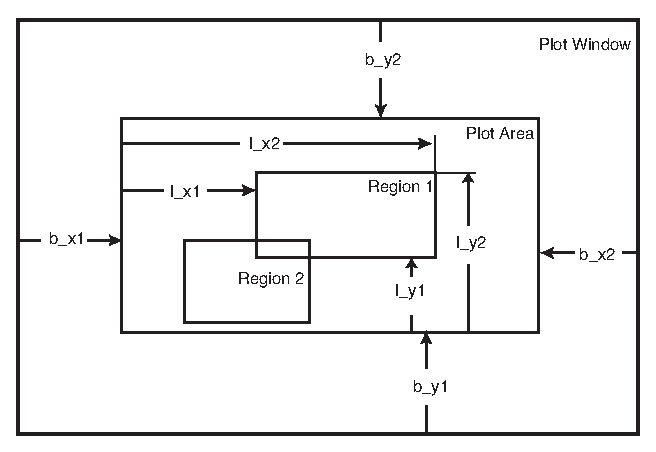
\includegraphics{plot_page.psfig}
  \caption{Regions define where on the plot page plots are placed.}
  \label{f:plot_page}
\end{figure}

Plotting is defined by an initialization file named
\vn{tao_plot.init}.  The first namelist block in the file has a block
name of \vn{tao_plot_page}. This block sets the size of the plot
window (also called the plot page) and defines the ``regions'' where
plots go. The syntax of this block is:
\index{tao_plot_page}    
\index{plot_page!size}
\index{plot_page!border}
\index{plot_page!text_height}
\index{plot_page!title}
\index{region!name}
\index{region!location}
\index{place}
\begin{example}
  &tao_plot_page
    plot_page%size        = <x_size>, <y_size>         ! size in POINTS 
    plot_page%border      = <b_x1>, <b_x2>, <b_y1>, <b_y2>, "<units>"
    plot_page%text_height = <text_height>              !height in POINTS
    plot_page%title(i)    = <string>, {<x>, <y>, "<justify>", "<units>"}
    region(i)%name        = "<region_name>"
    region(i)%location    = <l_x1>, <l_x2>, <l_y1>, <l_y2>  ! % plot area
    place(i)              = "<region>", "<template>"
  /
\end{example}
For example:
\begin{example}
  &tao_plot_page
    plot_page%size        = 700, 800           ! Points
    plot_page%border      = 0, 0, 0, 50, "POINTS"  
    plot_page%text_height = 12.0
    plot_page%title(1)    = "CESR Lattice"
    region(1)%name        = "top"
    region(1)%location    = 0.0, 1.0, 0.5, 1.0
    region(2)%name        = "bottom"
    region(2)%location    = 0.0, 1.0, 0.0, 0.5
    place(1)              = "top", "orbit"
    place(2)              = "bottom", "phase"
  /
\end{example}

\vn{plot_page%size} sets the horizontal and vertical size of the plot
window in \vn{POINTS} units (72 points = 1 inch. Roughly 1 point = 1
pixel). 

\vn{plot_page%border} sets a border around the edges of the
window. As shown in Figure~\ref{f:plot_page} \vn{b_x1}, \vn{b_x2} are
the right and left border widths and \vn{b_y1} and \vn{b_y2} are the
bottom and top border widths respectively.  The rectangle within this
border is called the plot area.

\vn{plot_page%title(i)} set the page title. There are two title areas 
(i = 1,2). If only the title string is given then the other variables 
are set to the defaults \vn{x} = 0.5, \vn{y} = 0.995, \vn{justify} = 
"CC" and \vn{units} = "%PAGE". See the quickplot documentation for 
the \vn{justify} variable syntax.

The plot area is divided up into rectangular regions where plots may
be placed (what defines a plot is discussed below).
\vn{region(i)%name} is the name of a region and my be any character
string. \vn{l_x1}, and \vn{l_x2} define the location of the left and
right edges of the region as a fraction of the plot area width
starting from the left edge of the plot area.  \vn{l_y1} and \vn{l_y2}
define the location of the bottom and top edges of the region as a
fraction of the height of the plot area with respect to the plot
area's bottom edge. Thus, in the above example, region 1 extends from
the left border of the plot area (\vn{region(1)%l_x1} = 0) to the
right border (\vn{region(1)%l_x2} = 0) and vertically from the center
(\vn{region(1)%l_y1} = 0.5) to the top edge (\vn{region(1)%l_x2} =
1.0). Regions may overlap any one can define as many regions as one
likes.

\vn{place(i)} determines the initial placement of plots.

%-----------------------------------------------------------------
\subsection{Templates}\index{Initialization!Plotting!Templates}

As shown in Figure~\ref{f:plot}, a ``plot'' is made up of a collection
of ``graphs'' and a graph consists of axes plus a set of ``curves''.
In the \vn{tao_plot.init} file there needs to be defined a set of
``template plots''. A template plot specifies the layout of a plot:
How the graphs are placed within a plot, what curves are associated
with what graphs, etc. When running \tao, the information in a
template plot may then be transfered to a region using the \vn{place}
command and this will produce a visible plot.

Template plots are defined using namelists with a name of
\vn{tao_template_graph}. The general syntax is:
\index{tao_template_plot}
\index{plot!name}
\index{plot!x}
\index{plot!x_axis_type}
\index{plot!ix_universe}
\index{plot!n_graph}
\index{plot!independent_graphs}
\begin{example}
  &tao_template_plot
    plot%name        = "<plot_name>"
    plot%x           = <qp_axis_struct>
    plot%x_axis_type = "<x_axis_type>"   ! "index" or "s". Default is "index".
    plot%ix_universe = <number> ! used for lat_layout plots
    plot%n_graph     = <n_graphs>
    plot%independent_graphs = <logical>  ! scale graph y-axis independently
  /
\end{example}
For example:
\begin{example}
  &tao_template_plot
    plot%name        = "orbit"
    plot%x%min       =   0
    plot%x%max       = 100
    plot%x%major_div = 10
    plot%x%label     = "Index"
    plot%n_graph     = 2
  /
\end{example}

\vn{plot%x} sets the properties of the horizontal axis. For more
information see the \vn{Quick Plot} documentation on the
\vn{qp_axis_struct}. The major components are
\index{qp_axis_struct!min}
\index{qp_axis_struct!max}
\index{qp_axis_struct!major_div}
\index{qp_axis_struct!minor_div}
\index{qp_axis_struct!label}
\begin{example}
  min        ! Left edge value.
  max        ! Right edge value.
  major_div  ! Number of major divisions. 
             !  Number of major tick marks is one less.
  minor_div  ! Number of minor divisions. 0 = auto choose.
  label      ! Axis label.
\end{example}

\vn{plot%name} is the name that is used with \tao commands to identify
the plot.  

\vn{plot%x_axis_type} sets what is plotted along the
\vn{x-axis}. Possibilities are:
\index{index}
\index{ele_index}
\index{s}
\begin{example}
    "index"      ! Data Index
    "ele_index"  ! Element lattice number index
    "s"          ! Longitudinal position in the lattice.
\end{example}

\vn{n_graph} sets the number of graphs associated with the plot and
each one needs a \vn{tao_template_graph} namelist to define it. These
namelists should be placed directly after their respective
\vn{tao_template_graph} namelists. The general format of the
\vn{tao_template_graph} namelist is:
\index{tao_template_graph}\index{graph!y}\index{curve!name}
\index{graph_index}\index{graph}\index{graph!name}\index{curve}
\index{graph!type}\index{graph!box}\index{graph!title}\index{graph!margin}
\index{graph!y2}\index{graph!n_curve}\index{graph!clip}\index{graph!who}
\index{curve!data_type}\index{curve!data_source}
\index{curve!x_axis_units_factor}\index{curve!y_axis_units_factor}
\index{curve!use_y2}\index{curve!line}\index{curve!ele_ref_name}
\index{curve!draw_line}\index{curve!draw_symbols}\index{curve!ix_universe}
\index{curve!symbol}\index{curve!symbol_every}\index{curve!convert}
\begin{example}
  &tao_template_graph
    graph_index           = <number>
    graph%name            = "<graph_name>"
    graph%type            = "<graph_type>"
    graph%box             = <ix>, <iy>, <ix_tot>, <iy_tot>
    graph%title           = "<label>''
    graph%margin          =  <ix1>, <ix2>, <iy1>, <iy2>, "<Units>"
    graph%y               = <qp_axis_struct>
    graph%y2              = <qp_axis_struct>
    graph%n_curve         = <number_of_curves>
    graph%clip            = <logical> ! Clip plot at grpah boundary. default = .true.
    graph%who(i)          = "<who_to_plot>", <sign>
    curve(i)%name         = "<curve_name>"
    curve(i)%data_type    = "<data_type>"
    curve(i)%data_source  = "<source_name>" !source for the data curve points
    curve(i)%x_axis_scale_factor = <factor> ! scale the x-axis by this.
    curve(i)%y_axis_scale_factor = <factor> ! scale the y-axis by this.
    curve(i)%use_y2       = <logical> 
    curve(i)%draw_line    = <logical>
    curve(i)%draw_symbols = <logical>
    curve(i)%ix_universe  = <universe_number> ! default = 0 => use viewed universe
    curve(i)%line         = <qp_line_struct>
    curve(i)%symbol       = <qp_symbol_struct>
    curve(i)%symbol_every = <integer>       ! plot symbol every # datums
    curve(i)%convert      = <Logical>
    curve(i)%draw_interpolated_curve = <Logical>
    curve(i)%ele_ref_name = "<element_name>"     ! reference element.
  /
\end{example}
For example:
\begin{example}
  &tao_template_graph
    graph_index           = 1
    graph%name            = "x"
    graph%type            = "data"
    graph%box             = 1, 1, 1, 2
    graph%title           = "Horizontal Orbit (mm)"
    graph%margin          =  60, 200, 30, 30, "POINTS"
    graph%y%label         = "X"
    graph%y%max           =  4
    graph%y%min           = -4
    graph%y%major_div     = 4
    graph%n_curve         = 1
    graph%who(1)          = "model", +1
    graph%who(2)          = "design", -1
    curve(1)%data_source  = 'data_array'
    curve(1)%data_type    = "orbit.x"
    curve(1)%units_factor = 1000
    curve(1)%use_y2       = .false.
  /
\end{example}

\vn{graph%name} and \vn{curve%name} define names to be used with
commands. The default names are just the letter \vn{g} or \vn{c} with
the index of the graph or
curve. Thus, in the example above, the name of the curve defaults to
\vn{c1} and it would be referred to as \vn{orbit.x.c1}.

\vn{graph%who(i)} sets what is plotted. In the above example, what will be
plotted is \vn{model - design}. Possible \vn{graph%who}
settings are:
\index{model}\index{design}\index{base}\index{meas}\index{ref}
\begin{example}
  "model"     ! model values.
  "design"    ! design values.
  "base"      ! Base values
  "meas"      ! data values.
  "ref"       ! reference data values.
\end{example}
The default, if \vn{graph%who} is not
specified, is for the graph will show \vn{model} values. 

\vn{graph%type} is the type of graph. \tao knows about the
following types:
\index{data}\index{lat_layout}\index{key_table}\index{phase_space}
\begin{example}
  "data"         ! Data plots (default) 
  "floor_plan"   ! A 2-dimentional birds-eye view of the machine.
  "key_table"    ! Key binding table for single mode.
  "lat_layout"   ! Schematic showing placement of the lattice elements.
  "phase_space"  ! Phase space plots
\end{example}
The \vn{key_table} is drawn with respect to the upper left hand corner
of the region in which it is placed.

\vn{graph%box} sets the layout of the box which the \vn{graph} is
placed in. For a definition of what a box is see the Quick Plot
documentation in the \bmad reference manual. In the above example the
graph divides the region into two vertically stacked boxes and places
itself into the bottom one. 

\index{data_array}\index{var_array}\index{calculation}
\index{curve!data_source}
The \vn{curve} structure is used to define the number and types of
curves to plot in each graph. \vn{curve%data_source} is the type of
information for the source of the data points. There are the following
types of data sources:
\begin{example}
  "data_array"       ! A d1_data array is the source of the curve points.
  "var_array"        ! A v1_var array is the source of the curve points.
  "calculation"      ! The curve points are computed directly from the lattice.
  "beam_calculation" ! The curve points are computed tracking a beam of particles.
\end{example}
With \vn{curve%data_source} set to \vn{data_array}, the values of the
curve points come from the \vn{d1_data} array structure named by
\vn{curve%data_type}. Thus in the above example the curve point values
are obtained from \vn{orbit.x} data. To be valid the data structure
named by \vn{curve%data_type} must be set up in an initialization
file. Similarly, \vn{var_array} indicates that the values of the curve
points come from a \vn{v1_var} array structure. \vn{calculation} means
that the curve data points are calculated from the lattice without
regard to any data structures. \vn{beam_calculation} is used when
tracking beams of particles or macroparticles. In this case the curve
points are calculated from the tracking. For example, with
\vn{curve%data_type} set to \vn{beta.x}, the setting of
\vn{curve%data_source} to \vn{calculation} gives the beta as
calculated from the lattice and \vn{beam_calculation} gives the beta
as calculated from the shape of the beam. 

For a curve with the \vn{curve%data_source} set to \vn{"data_array"} the
possible \vn{curve%data_type} values are the same as the possible
\vn{d1_data%type} values as given in \sref{s:data_types}. If the
\vn{curve%data_source} is \vn{"var_array"} then the possible
\vn{curve%data_type} values are any of the \vn{v1_var} names. This is
what points the curve to the proper data so there needs to be a
corresponding data or var type defined in the initialization file.  If
\vn{graph%type} is \vn{"phase_space"} then \vn{curve%data_source}
determines what planes are plotted. A plane is either:
\index{x}\index{p_x}\index{y}\index{p_y}\index{z}\index{p_z}
\begin{example}
  "x"
  "p_x"
  "y"
  "p_y"
  "z"
  "p_z"
\end{example}
For example:
\begin{example}
  curve%data_type = "x-p_x"  ! x-axis - y-axis
\end{example}
The dash \vn{-} is mandatory as the separator between the plane names. 

\vn{curve%convert} is a logical that is only used
with \vn{curve%data_name} = "coupling" and tells \tao to convert the
coupling data into cbar data before plotting.

\vn{curve%draw_symbols} determines whether a symbol is drawn at the
data points. The size, shape and color of the symbols is determined by
\vn{curve%symbol}.

\vn{curve%draw_line} determines whether a curve is drawn through the
data points. The thickness, style (solid, dashed, etc.), and color
is determined by \vn{curve%line}

%-----------------------------------------------------------------
\subsection{Lattice Layout}\index{Initialization!Lattice Layout}

A lattice layout template plot may be defined that draws the lattice
along a straight line with figures for the various elements.
The \vn{tao_template_plot} needed to define a lattice layout looks like:
\index{tao_template_plot}\index{plot!name}\index{plot!box_layout}
\index{plot!x!min}\index{plot!x!max}\index{plot!n_graph}
\index{tao_template_graph}\index{graph_index}\index{graph!name}
\index{graph!type}\index{graph!title}\index{graph!box}
\index{graph!ix_universe}\index{graph!margin}\index{graph!n_curve}
\begin{example}
  &tao_template_plot
    plot%name        = "<plot_name>"
    plot%box_layout  = <ix>, <iy> 
    plot%x%min       = <number>
    plot%x%max       = <number>
    plot%n_graph     = <number>
  /
  &tao_template_graph
    graph_index       = <number>
    graph%name        = <name>
    graph%type        = "lat_layout"
    graph%title       = "Layout Title"
    graph%box         = <ix>, <iy>
    graph%ix_universe = <integer> ! 0 => use currently viewd universe
    graph%margin      = <ix1>, <ix2>, <iy1>, <iy2>, "<Units>"
    graph%n_curve     = 0
  /
\end{example}
Example:
\begin{example}
  &tao_template_plot
    plot%name       = 'layout'
    plot%x%min      =   0
    plot%x%max      = 100
    plot%n_graph    = 1
  /

  &tao_template_graph
    graph_index       = 1
    graph%name        = 'u1'
    graph%type        = 'lat_layout'
    graph%this_box    = 1, 1
    graph%ix_universe = 1
    graph%margin      = 0.12, 0.12, 0.12, 0.12, '%BOX'
    graph%n_curve     = 0
  /
\end{example}

\index{element_shapes}
\index{shape}
With a \vn{graph%type} of \vn{lat_layout} or \vn{floor_plan}, 
the shapes to be drawn for the various lattice elements need to
be defined using an \vn{element_shapes} namelist whose syntax is:
\begin{example}
  &element_shapes 
    shape(i) = "<key>", "<name>", "<shape>", "<color>", 
                                      "<v_size>", "<print_Label>"
  /
\end{example}
For Example:                 
\begin{example}
  &element_shapes
    shape(1) = "Quadrupole", "Q*",      "Box",  "Red",      30,   T 
    shape(2) = "Quadrupole", "*",       "XBox", "Red",      30,   F 
    shape(3) = "SBend",      "*",       "Box",  "Blue",     15 
    shape(4) = "Wiggler",    "*",       "XBox", "Green",    20 
  /
\end{example}

A figure is drawn for each element in the lattice that matches a
shape. A Match is made if the type of element matches the shape
\vn{<key>} and the name of the element matches the shape
\vn{<name>}. The wildcard ``*'' may be used to denote any number of
characters. Thus, in the example above, \vn{shape(1)} will match to
all quadrupoles whose name begins with ``Q'' and \vn{shape(2)} will
match all quadrupoles. If an element matches more than one shape the
first shape matched will be used. \vn{<shape>} is the shape of the
figure drawn. Valid Shapes are:
\index{box}\index{xbox}
\begin{example}
  "BOX"             -- Rectangular box
  "XBOX"            -- Rectangular box with an x through it.
  "VAR_BOX"         -- Rectangular box with variable height. 
                        The box is symmetric about the center line.
  "ASYM_VAR_BOX"    -- Like VAR_BOX but is not symmetric about the center line. 
\end{example}
The height of a \vn{VAR_HEIGHT_BOX} is proportional to the element
strength. For example, for a quadrupole the height is proportional to
the \vn{K1} focusing strength. Not all elements can be used with a
\vn{VAR_HEIGHT_BOX}.

\vn{<color>} is the color of the shape. Good colors to use are:
\index{black}\index{Red}\index{orange}\index{magenta}\index{yellow}
\index{green}\index{cyan}\index{blue}\index{purple}
\begin{example}
  "BLACK"
  "RED"
  "ORANGE"
  "MAGENTA"
  "YELLOW"
  "GREEN"
  "CYAN"
  "BLUE"
  "PURPLE"
\end{example}
\vn{<v_size} is the vertical size of the shape in points (72 points =
1 inch). Finally \vn{<print_label>} is a logical indicating whether
the element name is to be printed underneath the figure.



%-----------------------------------------------------------------
\section{Initializing Key Bindings for Single Mode}\index{Initialization!Key Bindings}
\label{s:init_single} 

For single mode the bindings of variables to keys is defined with a
\vn{key_bindings} namelist. There is a maximum of 500 key bindings.
The syntax is:
\index{key_bindings}
\index{key}
\begin{example}
  &key_bindings
    key(i) = <ele_name> <attrib_name> <delta> <universe> 
          <small_step> <low_lim> <high_lim> <weight> <good_opt> <merit_type>
  /
\end{example}
For example:
\begin{example}
  &key_bindings
  key(1) = "Q1"   "K1"    0.01 "U:*" 1e-5  -10  10  10  T
  key(2) = "DRFT" "L"     0.1  "U:1" 1e-3    0   3   1  F
  key(3) = "Q3"   "TILT"  0.01 "U:2" 1e-5   -1   1   3  T "target"
  /  
\end{example}
For the \vn{i}\Th key \vn{<ele_name>} is the name of a lattice element
in universe \vn{<universe>} and \vn{<attrib_name>} is the attribute to
be varied. If \vn{<universe>} is ``0'' then the key will vary elements
in all universes. \vn{<delta>} is the change in value when the
appropriate key is depressed. \vn{<small_step>} establishes what a 
``small'' variation of the variable is. 

\vn{merit_type} sets the variable merit is calculated. See
\sref{s:init_var} for more details. the \vn{global%default_key_merit_type} 
sets the default \vn{merit_type}.

If \vn{merit_type} is \vn{"limit"} then \vn{<low_lim>} and
\vn{<high_lim>} establish limits and if the value of the variable goes
outside these limits then the contribution to the merit function is
given by
\index{merit function}
\begin{example}
  merit = <weight> * (var_value - <high_lim>)^2  ! For var_value > <high_lim>
  merit = <weight> * (<low_lim> - var_value)^2   ! Fro <low_lim> > var_value
\end{example}

%---------------------------------------------------------------------------------------------------------------
%---------------------------------------------------------------------------------------------------------------
% WARNING! If you are modifying this file, be aware that the online help system depends upon the lines starting 
% with "%%" to match blocks of text in this file with a given command. 
%
% The online help system also makes some further assumptions about how this file is formatted.
% Please test any modifications by running Tao and using the appropriate help command to see how
% your modifications translate. 
% Note: The translation code is at: 
%     tao/code/tao_help.f90
%---------------------------------------------------------------------------------------------------------------
%---------------------------------------------------------------------------------------------------------------

\chapter{Commands}
\label{c:command}
\index{commands!Command list} 

\tao has two \vn{modes} for entering commands. In \vn{line mode}'', described in this chapter, \tao
waits until the \vn{return} key is depressed to execute a command. That is, a command consists of a
single line of input. Conversely, \vn{Single Mode}, which is described in \vn{Single Mode} chapter
(\sref{c:single}), interprets each keystroke as a command. Single Mode is useful for quickly varying
parameters to see how they affect a lattice but the number of commands in Single Mode is limited. To
put \tao into \vn{single mode} use the \vn{single_mode} command (\sref{s:sing}).

The syntax for \vn{line mode} commands is discussed in Section~\sref{s:com.syntax}. The list of
commands is shown in Table~\ref{t:commands}.

This chapter uses the following special characters to define the command line syntax:
\begin{example}
  \{\}        ! Identifies an optional argument.
            !   Arguments now enclosed in brackets are required
  <>        ! Indicates a non-literal argument.
\end{example}

Example:
\begin{example}
  change \{-silent\} variable <name>[<locations>] <number>
\end{example}
Here the \vn{-silent} argument is optional while the \vn{variable} argument is mandatory.
Appropriate values for \vn{<name>}, \vn{<locations>}, and \vn{<number>} must be substituted. A
possible

\begin{example}
  change var steering[34:36] @1e-3  ! set the steering strength #34-36 to 0.001
\end{example}

%% command_table -----------------------------------------------------

\begin{table}[h]
\centering {\tt
\begin{tabular}{ll|ll} \toprule
  {\it Command} & {\it Section}     & {\it Command} & {\it Section}     \\ \midrule
  alias         & \sref{s:alias}    & re_execute    & \sref{s:re.exe}   \\
  call          & \sref{s:call}     & read          & \sref{s:read}     \\
  change        & \sref{s:change}   & reinitialize  & \sref{s:reinit}   \\ 
  clear         & \sref{s:clear}    & restore       & \sref{s:restore}  \\ 
  clip          & \sref{s:clip}     & run_optimizer & \sref{s:run}      \\ 
  continue      & \sref{s:continue} & scale         & \sref{s:scale}    \\ 
  create        & \sref{s:create}   & set           & \sref{s:set}      \\  
  cut_ring      & \sref{s:cut.ring} & show          & \sref{s:show}     \\ 
  derivative    & \sref{s:deriv}    & single_mode   & \sref{s:sing}     \\ 
  do, enddo     & \sref{s:do}       & spawn         & \sref{s:spawn}    \\ 
  end_file      & \sref{s:end.file} & taper         & \sref{s:taper}    \\
  exit          & \sref{s:exit}     & timer         & \sref{s:timer}    \\
  flatten       & \sref{s:flatten}  & use           & \sref{s:use}      \\ 
  help          & \sref{s:help}     & veto          & \sref{s:veto}     \\ 
  ls            & \sref{s:ls}       & view          & \sref{s:view}     \\
  pause         & \sref{s:pause}    & wave          & \sref{s:wave}     \\
  pipe          & \sref{s:pipe}     & write         & \sref{s:write}    \\
  place         & \sref{s:place}    & x_axis        & \sref{s:x.axis}   \\ 
  ptc           & \sref{s:ptc}      & x_scale       & \sref{s:x.scale}  \\ 
  python        & \sref{s:python}   & xy_scale      & \sref{s:xy.scale} \\ 
  quit          & \sref{s:quit}     &               &                   \\
\bottomrule 
\end{tabular}}
\caption{Table of \tao commands.}
\label{t:commands}
\end{table}

When running \tao, use the \vn{help} (\sref{s:help}) command to show documentation on any command.
For example, \vn{help plot} will show documentation on the \vn{plot} command.

%% Marker: "help" (with no arguments) will not display anything after this line -----------

\vfil
\break

%% alias --------------------------------------------------------------
\section{alias}\index{commands!alias}
\label{s:alias}

The \vn{alias} command defines command shortcuts. Format:
\begin{example}
  alias \{<alias_name> <string>\}
\end{example}

\vskip 7pt 

\vn{Alias} is like Unix aliases. Using the \vn{alias} command without any arguments
results in a printout of the aliases that have been defined. When using an alias up to 9 arguments
may be substituted in the \vn{<string>}. The i\Th argument is substituted in place of the sub-string
``[[i]]'' or ``[<i>]''.  Arguments that do not have a corresponding ``[[i]]'' or ``[<i>]'' are
placed at the end of \vn{<string>}. The difference between ``[[i]]'' and ``[<i>]'' is that ``[[i]]''
is a required argument while ``[<i>]'' defines an optional argument. For example
\begin{example}
  alias aaa show element [[1]] [[2]]
  alias zzz show element [[1]] [<2>]
\end{example}
This defines ``\vn{aaa}'' as an alias for the \vn{show element} command with two required arguments
while ``\vn{zzz}'' has only one requred argument.

Aliases can be set up for multiple commands using semicolons.

Examples:
\begin{example}
  alias xyzzy plot [[1]] model  ! Define xyzzy
  alias                         ! Show all aliases
  xyzzy top                     ! Use an alias
  plot top model                ! Equivalent to "xyzzy top"
  xyzzy top abc                 ! Equivalent to "plot top model abc"
  alias foo  show uni; show top ! "foo" equivalent to "show uni; show top"
\end{example}
In the above example ``xyzzy'' is the alias for the string ``plot [[1]] model''.  When the
command xyzzy is used ``top'' is substituted for ``[[1]]'' in the string.

%% call --------------------------------------------------------------
\section{call}\index{commands!call}
\label{s:call}

The \vn{call} command opens a command file (\sref{s:command.files}) and executes the commands in
it. Format: 
\vskip 1pt
\begin{example}
  call <filename> \{<arg_list>\}
  call -no_calc \{<arg_list>\}
  call -ptc <filename>
\end{example}

\vskip 1pt 
The \vn{call} command without \vn{-ptc} is for running a set of \tao commands.  Up to 9
arguments may be passed to the command file. The i\Th argument is substituted in place of the string
``[[i]]'' in the file. Nesting of command files (command files calling other command files) is
allowed. There is no limit to the number of nested files.  See the \vn{Command Files and Aliases}
section (\sref{s:command.files}) for more details.

The \vn{call -ptc} command passes the command file to PTC for processing. Previous to such a call,
the command \vn{ptc init} must be issued. This is for PTC wizards only.

If a command file calls another command file, and the name of the second command file has a relative
(as opposed to absolute) path name, \tao will look for the second command file relative to the
directory of the first command file. To have \tao look relative to your current working directory
(where you started \tao), use the prefix \vn{\$PWD/}. For example, to call a command file that is
one level up from your current working directory use
\begin{example}
  call \$PWD/../second.cmd
\end{example}

Command loops can be implemented in a command file. See the documentation on \vn{do/enddo}
(\sref{s:do}) for more details.

The \vn{-no_calc} option is equivalent to putting the following at the beginning of the
command file to speed up execution time:
\begin{example}
  set global lattice_calc_on = F   ! Stop lattice calculations (\sref{s:lat.calc}).
  set global plot_on = F           ! Halt replotting 
or
  set calc off                     ! Same as the two lines above.
\end{example}
When using the \vn{-no_calc} option, at the end of the command file the \vn{lattice_calc_on} and
\vn{plot_on} logicals will be toggled back to their initial values.

To suppress all the output when running a command file use the command:
\begin{example}
  set global quiet = all       ! Suppress everything except errors
  set global quiet = warnings  ! Suppress just warnings.
  set global quiet = off       ! No suppression
\end{example}
Note: if \vn{quiet} is set in a command file, the setting will persist to the end of the file and then
revert to what it was before the command file was run.

Examples:
\begin{example}
    call -no my_cmd_file abc def 
\end{example}
In the above example the argument ``abc'' is substituted for any ``[[1]]'' appearing the
file and ``def'' is substituted for any ``[[2]]''.  \Newline

%% change * --------------------------------------------------------------
\section{change}\index{commands!change}
\label{s:change}

The \vn{change} command changes element attribute values or variable values in the \vn{model}
lattice. Format:
\begin{example}
  change \{-update\} element <element_list> <attribute> \{prefix>\} <number>
  change \{-silent\} variable <name>[<locations>] \{<prefix>\} <number>
  change \{n@\}particle_start <coordinate> \{prefix>\} <number>
  change \{-branch <branch_list>\} \{-listing\} \{-mask <veto_list>\} tune \{dQa\} \{dQb\}
  change \{-branch <branch_list>\} z_tune dQz
\end{example}

\vskip 10pt 
The \vn{change} is used for changing real (as opposed to integer or logical) parameters. Also
consider using the \vn{set} command (\sref{s:set}) which is more general.

If \vn{<prefix>} is not present, \vn{<number>} is added to the existing value
of the attribute or variable. That is:
\begin{example}
  final_model_value = initial_model_value + <number>
\end{example}
If \vn{<prefix>} is present, it may be one of
\begin{example}
  @       final_model_value = <number>
  d       final_model_value = design_value + <number>
  \%       final_model_value = initial_model_value * (1 + <number> / 100)
\end{example}

Element list format (\sref{s:ele.list.format}), without any embedded blanks, is used for
the \vn{<element_list>} argument.

For \vn{change particle_start}, The optional \vn{n@} universe specification (\sref{s:universe}) may
be used to specify the universe or universes to apply the change command to.

For lattices with an open geometry, \vn{change particle_start <coordinate> <number>} can be used to
vary the starting coordinates for single particle tracking. If the \vn{use_particle_start} of the
\vn{beam_init} structure (\sref{s:beam.init}) is set to True, \vn{particle_start} will also vary the
beam centroid and the beam particle spin for tracking. Here \vn{<coordinate>} is one of:
\begin{example}
  x, px, y, py, z, pz, t
\end{example}
For photons, \vn{<coordinate>} may also be:
\begin{example}
  e_photon, field_x, field_y, phase_x, phase_y
\end{example}
For closed lattices only the \vn{pz} component is applicable. For lattices that have an \vn{e_gun}
(which necessarily implies that the lattice has an open geometry), the time \vn{t} coordinate must
be varied instead of \vn{pz}.

For open lattices, \vn{change element beginning <twiss>} can be used to vary the starting Twiss
parameters where \vn{<twiss>} is one of:
\begin{example}
  beta_a, beta_b, alpha_a, alpha_b 
  eta_a, eta_b,etap_a, etap_b    
\end{example}

The \vn{change z_tune} command will vary the longitudinal tune by \vn{<dQz>}. The \vn{<branch_list>}
is used to select which lattice branches the tune is varied in. Each branch listed can have an
optional universe prefix. The default is to vary branch 0 of the current default universe.

The \vn{change tune} command will vary the transverse tunes by \vn{<dQa>} and \vn{<dQb>} and 
the \vn{change z_tune} command will vary the longitudinal tune by \vn{<dQz>}. Units are in radians/2pi
With the \vn{change tune} command, if \vn{<dQa>} or \vn{<dQb>} is not given, the value will
be taken to be zero (that is, no change). The \vn{<branch_list>} is a list of lattice
branches with optional universe prefix, to vary the tunes. The \vn{<veto_list>} of the \vn{-mask}
option gives a list of quadrupoles {\em not} to use for varying the tune. See the \vn{set tune}
(\sref{s:set.tune}) command for more details. The \vn{-listing} option, if present, will, in
addition to the tune change, generate a list of quadrupoles varied along with variation
coefficients.

The \vn{-silent} switch, if present, suppresses the printing of what variables are changed.

The \vn{-update} switch, if present, suppresses \tao from printing error messages if a ``variable
slave value mismatch'' is detected (\sref{s:var.mismatch}). Independent of whether \vn{-update} is
present or not, \tao will fix the mismatch using the changed value to set all of the slave values.

Note: The \vn{change element} command can be used with \vn{ramper} type elements.

Examples:
\begin{example}
  change ele 3@124 x_offset 0.1        ! Offset element #124 in universe 3 by 0.1
  change ele 1,3:5 x_offset 0.1        ! Offset elements 1, 3, 4, and 5 by 0.1
  change ele q* k1 d 1.2e-2            ! Set the k1 strength of all elements starting with
                                       !   the letter "q" relative to the design
  change ele quadrupole::* k1 d 1.2e-2 ! Set the k1 strength of all quadrupole elements.
  change var steering[34:36] @1e-3     ! set the steering strength #34-36 to 0.001
  change var steering[*] \%10           ! vary all steering strengths by 10\%
  change 2@particle_start x @0.001     ! set beginning x position in universe 2 to 1 mm.
  change -mask Q1* tune 0 0.01         ! Change transverse tunes without using quadrupoles
                                       !   whose names start with "Q1".
  change -branch 2@1 z_tune 0.02       ! Change z-tune of branch #1 of universe #2.
\end{example}


%% clear --------------------------------------------------------------
\section{clear}\index{commands!clear}
\label{s:clear}

The \vn{clear} command clears stored spin and orbital Taylor maps from all elements in a lattice
with the exception of \vn{Taylor} elements (which are specified in the lattice file as opposed to
being calculated by \bmad). Format:
\begin{example}
  clear maps
\end{example}

Clearing the Taylor maps may be needed if the maps are in use (for example, with a spin polarization
calculation) and orbit excursions place the calculated orbit outside of the range of validity of the
maps.

%% clip --------------------------------------------------------------
\section{clip}\index{commands!clip}
\label{s:clip}

The \vn{clip} command vetoes data points for plotting and optimizing. That is, the \vn{good_user}
logical of the data associated with the out-of-bound plotted points are set to False.  Format:
\begin{example}
  clip \{-gang\} \{<where> \{<limit1> \{<limit2>\}\}\}
\end{example}

\vskip 10pt Which graphs are clipped is determined by the \vn{<where>} switch. If \vn{<where>} is
not present, all graphs are clipped. If \vn{where} is a plot name, then all the graphs of that plot
are clipped. If \vn{where} is the name of a \vn{d2_data} (for example, \vn{orbit}) or a \vn{d1_data}
(for example, \vn{orbit.x}) structure, then those graphs that display this data are clipped.

The points that are clipped those points whose $y$ values are outside a certain range defined by
\vn{<limit1>} and \vn{<limit2>}. If neither \vn{<limit1>} nor \vn{<limit2>} are present, the clip
range is taken to be outside the graph minimum and maximum $y$--axis values. If only \vn{<limit1>}
is present then the clip range is outside the region from -\vn{<limit1>} to +\vn{<limit1>}. If both
are present than the range is from \vn{<limit1>} to \vn{<limit2>}.

The \vn{-gang} switch is apply a clip to corresponding data in a \vn{d2_data} structure. For example
\begin{example}
  clip -g orbit.x   ! Clips both orbit.x and orbit.y 
\end{example}
Here the \vn{orbit.x} data is clipped and the corresponding data in \vn{orbit.y} is also vetoed. For
example, if datum number 23 in \vn{orbit.x} is clipped, datum number 23 in \vn{orbit.y} will be
vetoed.

Examples:
\begin{example}
  clip top.x -3  7  ! Clip the curves in the x graph in the region named "top".
  clip bottom       ! Clip the graphs in the "bottom" region
  clip -g orbit.x   ! Clip the orbit.x graph and also veto corresponding points
                    ! in other graphs of the orbit plot.
\end{example}

%% create --------------------------------------------------------------
\section{create}\index{commands!create}
\label{s:create}

Format:
\begin{example}
  create data ... ! \sref{s:create.data}
\end{example}

The \vn{create} command constructs various tao objects that would have
otherwise been created in tao initialization. 

% Use the command:
%   help create <subcommand>
% to obtain more information on a particular write subcommand. Example:
%   help create data

%% create data --------------------------------------------------------------

\subsection{create data}
\label{s:create.data}

The \vn{create data} constructs a new \vn{d2_data} and one or more \vn{d1_data} for it.
The primary purpose of this command is to make more data available for design
and optimization in an interactive session; for repeated use, create data using
data initialization namelists (\sref{s:init.data}). The resulting data must be
initialized with the \vn{set data} command (\sref{s:set.data}).

Syntax:
\begin{example}
  create data d2_name d1_name[ix_min:ix_max] ...
\end{example}

You may have as many \vn{d1_name}s as needed.
\vn{ix_min} and \vn{ix_max} must be literal integers, not expressions.

%% cut_ring --------------------------------------------------------------
\section{cut_ring}\index{commands!cut_ring}
\label{s:cut.ring}

Format:
\begin{example}
  cut_ring \{-particle_start\} \{-static\} \{-zero\} 
\end{example}

The \vn{cut_ring} command is used to toggle the geometry of the viewed \vn{model} lattice between
\vn{closed} to \vn{open}.

When the lattice is toggled to an open geometry, the \vn{-particle_start}, \vn{-static} or
\vn{-zero} options can be used to set the starting orbit. In all cases, the starting orbit is set
equal to the setting of \vn{particle_start} where \vn{particle_start} can be set in the lattice file
and/or using \tao's \vn{set particle_start} or \vn{change particle_start} commands. 

With the \vn{-static} option (the default), \vn{particle_start} is set to the same orbit as
currently exists for the closed orbit. The exception is if no closed orbit is found. In this case,
\vn{particle_start} is not modified (same as with the \vn{particle_start} option).

With the \vn{-zero} option, the \vn{particle_start} orbit is set to zero. 

With the \vn{-particle_start} option, the \vn{particle_start} orbit is not modified.

\begin{example}
  cut -zero   ! When lattice geometry is toggled open: zero initial orbit.
\end{example}

%% continue --------------------------------------------------------------
\section{continue}\index{commands!continue}
\label{s:continue}

The \vn{continue} command is used to continue reading of a suspended command file
(\sref{s:command.files}) after a \vn{pause} command (\vn{s:pause}). Format:
\begin{example}
  continue
\end{example}

%% do --------------------------------------------------------------
\section{do/enddo command file looping}\index{commands!do}
\label{s:do}

Command loops can be implemented in a command file files. Format:
\begin{example}
  do <var> = <l_bound>, <u_bound> \{, <incr>\}
    ...   ! use the syntax ``[[<var>]]'' to refer to a variable.
  enddo
\end{example}
Note: ``\vn{enddo}'' is one word and my not be split into two words. Loops can be nested and the
number of levels is not unlimited.

A loop will execute the code in between the \vn{do} and \vn{enddo} lines a certain number of
times. Each time trough the the the integer variable \vn{<var>} will be incremented by \vn{<incr>},
starting at \vn{<l_bound>} and stopping before \vn{<var>} is greater than \vn{<u_bound>}. If
\vn{<incr>} is not present, the increment will be 1. Note: \vn{<l_bound>}, \vn{<u_bound>}, and
\vn{<incr>} must all be integers.

Example:
\begin{example}
  do j = 0, 10, 2
    set particle_start pz = 1e-3 * [[j]]
    ...
  enddo
\end{example}
As shown in the above example, to refer to a loop variable in a command, use the syntax ``[[<var>]]''.

%% end_file --------------------------------------------------------------
\section{end_file} \label{s:end.file}
\index{commands!end_file}

The \vn{end_file} command is used in command files (\sref{s:command.files}) to signal the end of the
file. Everything after an \vn{end_file} command is ignored. An \vn{end_file} command entered at the
command line will simply generate an error message.  Format:
\begin{example}
  end_file
\end{example}

%% exit --------------------------------------------------------------
\section{exit}\index{commands!exit}
\label{s:exit}

The \vn{exit} command exits the program. Same as \vn{Quit}.  Format:
\begin{example}
  exit
\end{example}

%% derivative --------------------------------------------------------------
\section{derivative}\index{commands!derivative}
\label{s:deriv}

The \vn{derivative} command calculates the \vn{dModel_Data/dVar} derivative matrix needed for the
\vn{lm} optimizer.  Format:
\begin{example}
  derivative
\end{example}

%% flatten --------------------------------------------------------------
\section{flatten}\index{commands!flatten}
\label{s:flatten}

The \vn{Flatten} command runs the optimizer to minimize the merit function. This is the same as the
\vn{run_optimizer} command.  See the \vn{run_optimizer} command for more details. Format:
\begin{example}
  flatten \{<optimizer>\}
\end{example}

\vskip 10pt

%% help --------------------------------------------------------------
\section{help}\index{commands!help}
\label{s:help}

The \vn{help} command gives help on \tao commands. Format:
\begin{example}
  help \{<command> \{<subcommand>\}\}
\end{example}

\vskip 10pt
The \vn{help} command without any arguments gives a list of all commands.  Some commands, like
\vn{show}, are so large that help on these commands is divided up by their subcommand.

Examples:
\begin{example}
  help            ! Gives list of commands.
  help run        ! Gives help on the run_optimizer command.
  help show       ! Help on the show command.
  help show alias ! Help on the show alias command.
\end{example}

The \vn{help} command works by parsing the file \vn{\$TAO_DIR/doc/command-list.tex} which is the
LaTeX file for the \vn{Tao Commands} chapter of the \tao manual. For the \vn{help} command to work
properly, the environment variable \vn{TAO_DIR} must be appropriately defined. Generally,
\vn{TAO_DIR} will be defined if the appropriate \bmad setup script has been run. For
``Distributions'', this is the same setup script used to setup a distribution. See your local \bmad
guru for details.

When the \vn{help} command parses the \vn{\$TAO_DIR/doc/command-list.tex} file, LaTeX syntax will be
modified to produce a reasonable looking output on the terminal. This translation is not perfect so
reference should be made to the \tao manual if there is a problem in the translation.

%% ls --------------------------------------------------------------
\section{ls}\index{command!ls}
\label{s:ls}

The \vn{ls} command is the same as the standard UNIX \vn{ls} command to display a list of files and
directories. The standard ls switches are accepted. This is equivalent to the \vn{spawn ls} command.
Format:
\begin{example}
  ls \{switches\}
\end{example}

Example:
\begin{example}
  ls -lrt
\end{example}

%% pause --------------------------------------------------------------
\section{pause}\index{commands!pause}
\label{s:pause}

The \vn{pause} command is used to pause \tao when executing a command file
(\sref{s:command.files}). Format:
\begin{example}
  pause \{<time>\} ! Pause time in seconds.
\end{example}

\vskip 10pt
If \vn{<time>} is not present or zero, \tao will pause until the \vn{CR} key is pressed. Once the
\vn{CR} key is pressed, the command file will be resumed. If \vn{<time>} is negative, \tao will
suspend the command file. Commands can now be issued from the keyboard and the command file will be
resumed when a \vn{continue} command (\sref{s:continue}) is issued. Multiple command files can be
simultaneously suspended.  Thus, while one command file is suspended, a second command file can be
run and this command file too can be suspended. A \vn{continue} command will resume the second
command file and when that command file ends, another \vn{continue} command will be needed to
complete the first suspended command file. Use the \vn{show global} command to see the number of
suspended command files.

Example:
\begin{example}
  pause 1.5    ! Pause for 1.5 seconds.
  pause -1     ! Suspend the command file until a \vn{continue} 
               !   command is issued.
\end{example}

%% pipe -----------------------------------------------------------
\section{pipe}\index{commands!pipe}
\label{s:pipe}

The \vn{pipe} command is like the \vn{show} command in that the \vn{pipe} command prints
information to the terminal. The difference is that the output from the \vn{show} command is meant
for viewing by the user while the output of the \vn{pipe} command is meant for easy
parsing. Format:
\begin{example}
  pipe \{-append <file_name>\} \{-noprint\} <subcommand> <arguments>
  pipe \{-write <file_name>\} \{-noprint\} <subcommand> <arguments>
\end{example}

The \vn{pipe} command has \vn{-append} and \vn{-write} optional arguments which can be used to
write the results to a file. The \vn{pipe -append} command will appended to the output file. The
\vn{pipe -write} command will first erase the contents of the output file. Example:
\begin{example}
  pipe -write d2.dat data_d2    ! Write to file "d2.dat"
\end{example}

The \vn{-noprint} option suppresses printing and is useful when writing large amounts of data to a
file.  The \vn{pipe} command can be used to pass information to a parent process when \tao is run
as a subprocess.  The parent process may be any scripting program like Pipe, Perl, Tcl, etc.  In
particular, see the \vn{Python Interface} chapter (\sref{c:python}) for details on how to run
\tao as a Python subprocess.

In terms of long term maintainability, the advantage of using the \vn{pipe} command in the scripts
over the \vn{show} command comes from the fact that the output syntax of \vn{show} commands can (and
does) change.

Note to programmers: For debugging, the \vn{show internal -pipe} command will show the \vn{c_real}
and \vn{c_integer} arrays.

Possible \vn{<subcommand>} choices are:
\begin{example}
  beam, beam_init, branch1, bunch_comb, bunch_params, bunch1, bmad_com, 
  building_wall_list, building_wall_graph, building_wall_point, 
  building_wall_section, constraints, da_params, da_aperture, 
  data, data_d2_create, data_d2_destroy, data_d_array, data_d1_array,
  data_d2, data_d2_array, data_set_design_value, data_parameter,
  datum_create, datum_has_ele, derivative, ele:ac_kicker, ele:cartesian_map,
  ele:chamber_wall, ele:control_var, ele:cylindrical_map, ele:elec_multipoles,
  ele:floor, ele:gen_grad_map, ele:grid_field, ele:gen_attribs, ele:head, ele:lord_slave, 
  ele:mat6, ele:methods, ele:multipoles, ele:orbit, ele:param, ele:photon, 
  ele:spin_taylor, ele:taylor, ele:twiss, ele:wake, ele:wall3d, em_field, enum,
  evaluate, floor_plan, floor_orbit, global, help, inum, lat_branch_list,
  lat_calc_done, lat_ele_list, lat_list, lat_param_units, matrix, merit, orbit_at_s,
  place_buffer, plot_curve, plot_graph, plot_histogram, plot_lat_layout, plot_line,
  plot_plot_manage, plot_graph_manage, plot_curve_manage, plot_list, plot_symbol,
  plot_transfer, plot1, ptc_com, ring_general, shape_list, shape_manage,
  shape_pattern_list, shape_pattern_manage, shape_pattern_point_manage, shape_set,
  show, species_to_int, species_to_str, spin_invariant, spin_polarization, 
  spin_resonance, super_universe, twiss_at_s, universe, var_v1_create, var_v1_destroy, 
  var_create, var_general, var_v1_array, var_v_array, var, wave
\end{example}

%% place --------------------------------------------------------------
\section{place}\index{commands!place}
\label{s:place}

The \vn{place} command is used to associate a \vn{<template>} plot with a \vn{<region>} and thus
create a visible plot in that region. Format:
\begin{example}
  place \{-no_buffer\} <region> <template>
  place <region> none
  place * none
\end{example}

\vskip 10pt 
If \vn{<region>} is set to ``\vn{*}'' then all regions are selected.

If \vn{<template>} is set to ``\vn{none}'' all selected regions are cleared of plots.

The \vn{-no_buffer} optional switch is used when external plotting is being done (EG with a GUI) and
is not of interest otherwise.

Notice that by using multiple \vn{place} commands a \vn{template} can be associated with more than
one region. For example, if multiple orbit plots are desired.

Examples:
\begin{example}
  place * none     ! Erase all plots.
  place top orbit  ! Place the orbit template in the top region
  place top none   ! Erase any plots in the top region
\end{example}

%% ptc -----------------------------------------------------------
\section{ptc}\index{commands!ptc}
\label{s:ptc}

The \vn{ptc} command is used manipulating PTC layouts associated with Bmad
lattices. Format:
\begin{example}
  ptc init            ! Init associated PTC layout.
  ptc reslice         !
\end{example}

\vskip 10pt 

The \vn{ptc init} command initializes a PTC layout.

The \vn{ptc reslice} command calculates good values for lattice element \vn{num_steps} and \vn{integrator_order}. This
command does not adjust the following elements since the algorithm for the calculation can be problematical when the field
is varying longitudinally within an element:
\begin{example}
  rfcavity, lcavity, crab_cavity
  wiggler, undulator
\end{example}

Also see:
\begin{example}
  call -ptc <file>         ! Run a PTC script
  read ptc                 ! Read a PTC lattice
  write ptc                ! Write a PTC lattice
\end{example}

Examples:
\begin{example}
  ptc init
\end{example}


%% python -----------------------------------------------------------
\section{python}\index{commands!python}
\label{s:python}

\vn{Python} is the old name for the \vn{pipe} command. For backwards compatibility,
the old name is still accepted.

%% quit --------------------------------------------------------------
\section{quit}\index{commands!quit}
\label{s:quit}

\vn{Quit} exits the program. Same as \vn{exit}.
Format:
\begin{example}
  quit
\end{example}

%% re_execute --------------------------------------------------------------
\section{re_execute}
\index{commands!re_execute}
\label{s:re.exe}

The \vn{re_execute} command reruns prior commands.  Format:
\begin{example}
  re_execute <index>   ! Re-execute a command with the given index number.
  re_execute <string>  ! Re-execute last command that begins with <string>.
\end{example}

\vskip 10pt 

Every \tao command entered is recorded in a ``history stack''. These commands can be viewed using
the \vn{show history} command. The \vn{show history} command will also display the index number
associated with each command.

Note: The up and down arrow keys on the keyboard can be used to scroll through the command history
stack.

Examples
\begin{example}
  re_exe 34   ! Re-execute command number 34.
  re_exe set  ! Re-execute last ``set'' command.  
\end{example}

%% read --------------------------------------------------------------
\section{read}\index{commands!read}
\label{s:read}

The \vn{read} command is used to modify the (\bmad) \vn{model} lattice or the associated \vn{PTC}
lattice. Format:
\begin{example}
  read lattice \{-silent\} \{-universes <universe-list>\} <file_name>
  read ptc <file_name>
\end{example}

\vskip 10pt 

With the \vn{read lattice} command, the \vn{model} lattices contained in the universes specified by
\vn{<universe-list>} are modified using a ``secondary lattice'' file.  [See the \bmad manual for the
definition of ``secondary lattice''.] For example, with the appropriate file, the \vn{read} command
can be used to misalign the lattice elements. For the \vn{read lattice} command, the input file must
be in Bmad standard lattice format.

If \vn{-universes} is not present, only the \vn{model} lattice
in the default universe is modified.

If, after the lattice file has been read in, a given \tao variable has slave parameters that have
different values there is a problem. For example, if a \tao variable controls the \vn{k2} value of
sextupoles elements \vn{S1} and \vn{S2}, and if \vn{S1} is set to a different value than \vn{S2},
there is an inconsistency which needs to be corrected. This can be done in a number of ways. For
example, by using the \vn{set ele -update} command or using a further \vn{read lattice} command with
a lattice that corrects the problem.

If desired, the \vn{-silent} switch can be used to suppress error messages about differing \tao
variable slave parameter values.

Note: Due to bookkeeping complications, the number of lattice elements may not be modified. If it is
desired to initiate \tao using both ``primary'' and secondary lattice files, this can be done as
illustrated in \sref{s:init.lat}.

The \vn{read ptc} command reads in a PTC lattice. WARNING: This command is untested. Please contact
David Sagan if you want to use it.

Examples:
\begin{example}
  read lat -uni * lat.bmad   ! Modify model lattice of all universes.
  read lat -uni 2,3 lat.bmad ! Modify model lattice universes 2 and 3.
\end{example}

%% reinitialize -------------------------------------------------------
\section{reinitialize}\index{commands!reinitialize}
\label{s:reinit}

The \vn{reinitialize} command reinitializes various things. Format:
\begin{example}
  reinitialize beam
  reinitialize data
  reinitialize tao \{-clear\} \{command line optional arguments\}
\end{example}

\vskip 10pt 

The \vn{reinitialize beam} command reinitializes the beam at the start of the lattice. That is, a
new random distribution is generated.  Note: This also reinitializes the model data.

\vn{reinitialize data} forces a recalculation of the model data.  Normally, a recalculation is done
automatically when any lattice parameter is changed so this command is generally only useful for
debugging purposes.

\vn{reinitializes tao} reinitializes \tao. This can be useful to reset everything to initial
conditions or to perform analysis with more than one initialization file. See the Command Line
Initialization section (\sref{s:command.line}) for a list of the optional arguments. If an argument
is not set, the \vn{reinitialize} command uses the same argument value that were used in the last
\vn{reinitialize} command, or, if this is the first reinitialization, what was used to start \tao.
Exception: If the \vn{-clear} switch is present, all initialization parameters are set to their
default state before the command line arguments specified in the \vn{reinitialize} command are
parsed. The \vn{-clear} switch, if used, should come before any command line arguments since if
there are command line arguments before the \vn{-clear} switch, these arguments will be cleared.

Examples:
\begin{example}
  reinit tao                         ! Reinit using previous arguments
  reinit tao -init special.init      ! Reinitializes \tao with the initialization file 
                                     !   special.init.
  reinit -clear -start my_start      ! Use default init values except for the start file.                    
\end{example}

%% restore --------------------------------------------------------------
\section{restore}\index{commands!restore}
\label{s:restore}

The \vn{restore} command cancels data or variable vetoes. Format:
\begin{example}
  restore data  <data_name> <locations>
  restore var <var_name> <locations>
\end{example}

\vskip 10pt 

See also the \vn{use} and \vn{veto} commands.

Examples:
\begin{example}
  restore data orbit.x[23,34:56]   ! un-veto orbit.x 23 and 34 through 56.
  restore data orbit.x[23,34:56:2] ! un-veto orbit.x 23 and even data between 34 
                                   !                                          and 56
  restore data *@orbit[34]         ! un-veto orbit data in all universes.
  restore var quad_k1[67]          ! un-veto variable
\end{example}

%% run --------------------------------------------------------------
\section{run_optimizer}\index{commands!run}
\label{s:run}

The \vn{run_optimizer} command runs an optimizer. Format:
\begin{example}
  run_optimizer \{<optimizer>\}
\end{example}

\vskip 10pt 

\index{de!optimizer}\index{lm!optimizer}
If \vn{<optimizer>} is not given then the default optimizer is used.  Use the \vn{show optimizer}
(\sref{s:show.optimizer}) command to see optimizer parameters.  To stop the optimizer before it is
finished press the period ``.''  key. If you want the optimizer to run forever run the optimizer in
\vn{single mode}. Valid optimizers are:
\begin{example}
  custom        ! Used when a custom optimizer has been implemented (\sref{c:custom.tao}).
  de            ! Differential Evolution (good for global optimizations).
  geodesic_lm   ! ``Geodesic'' Levenburg-Marquardt (good for local optimizations).
  lm            ! Levenburg-Marquardt (good for local optimizations).
  lmdif         ! Levenburg-Marquardt (alternative version) (good for local optimizations).
  svd           ! svd optimizer (good for local optimizations).
\end{example}

See the optimization chapter (\sref{c:opti}) for details on how \tao structures optimization and for
more details on the different optimizers.

Examples:
\begin{example}
  run         ! Run the default optimizer
  run de      ! Run the de optimizer
\end{example}

%% scale --------------------------------------------------------------
\section{scale}\index{commands!scale}
\label{s:scale}

The \vn{scale} command scales the vertical axis of a graph or set of graphs.  Format:
\begin{example}
  scale \{-exact\} \{-gang\} \{-include_wall\} \{-nogang\} 
             \{-y\} \{-y2\} \{<where> \{<value1> \{<value2>\}\}\}
\end{example}

Which graphs are scaled is determined by the \vn{<where>} switch. If \vn{<where>} is not present or
\vn{<where>} is \vn{all} then all graphs are scaled. \vn{<where>} can be a plot name or the name of
an individual graph withing a plot.

\vn{scale} adjusts the vertical scale of graphs. If neither \vn{<value1>} nor \vn{<value2>} is
present then an \vn{autoscale} is performed and the scale is adjusted so that all the data points
are within the graph region. If an autoscale is performed upon an entire plot, and if
\vn{plot%autoscale_gang_y} (\sref{s:template}) is True, then the chosen scales will be the same for
all graphs. That is, a single scale is calculated so that all the data of all the graphs is within
the plot region. The affect of \vn{plot%autoscale_gang_y} can be overridden by using the \vn{-gang}
or \vn{-nogang} switches.

If only \vn{<value1>} is present then the scale is taken to be from -\vn{<value1>} to +\vn{<value1>}.
If both are present than the scale is from \vn{<value1>} to \vn{<value2>}.

A graph can have a \vn{y2} (left) axis scale that is separate from the \vn{y} (right) axis.
Normally, the \vn{scale} command will scale both axes.  Scaling of just one of these axes can be
achieved by using the \vn{-y} or \vn{-y2} switches.

How a graph is scaled is determined in part by the setting of the \vn{bounds} parameter in the
\vn{y} and \vn{y2} components of the graph. See \vn{s:quick.plot} for more details. The \vn{-exact}
switch, if present, will set \vn{bounds} to \vn{"EXACT"} which means that \tao will use the min and
max bounds as given by \vn{<value1>} and \vn{<value2>} and not try to find ``nice'' values near the
given ones. If \vn{<value1>} and \vn{<value2>} are not given, and if \vn{bounds} is set to
\vn{"EXACT"}, \tao will set \vn{bounds} to \vn{"GENERAL"}. Note: To set the axis \vn{bounds}
directly, use the \vn{set graph} command.

For scaling \vn{floor_plan} plots where there is a building wall to be drawn, if \vn{-include_wall}
is present and autoscaling is being done, then the plot bounds are extended to include the extent of
the building wall.

Examples:
\begin{example}
  scale top.x -3  7  ! Scale the x graph in the top region
  scale -y2 top.x    ! Scale only the y2 axis of the top.x graph.
  scale bottom       ! Autoscale the graphs of the plot in the bottom region
  scale -include     ! Scale everything and include the extent of any 
                     !   building walls in the calculation of the plot bounds.
\end{example}


%% set --------------------------------------------------------------
\section{set}\index{commands!set}
\label{s:set}

The \vn{set} command is used to set values for data, variables, etc. Subcommands are:
\begin{example}
  set beam \{n@\}<parameter> = <value>                        ! \sref{s:set.beam}
  set beam_init \{n@\}<parameter> = <value>                   ! \sref{s:set.beam.init}
  set bmad_com <parameter> = <value>                        ! \sref{s:set.bmad.com}
  set branch <branch> <parameter> = <value>                 ! \sref{s:set.branch}
  set calculate <on/off>                                    ! \sref{s:set.calc}
  set curve <curve> <parameter> = <value>                   ! \sref{s:set.curve}
  set data <data_name>|<parameter> = <value>                ! \sref{s:set.data}
  set default <parameter> = <value>                         ! \sref{s:set.default}
  set dynamic_aperture \{n@\}<parameter = <value>             ! \sref{s:set.da}
  set element <element_list> <attribute> = <value>          ! \sref{s:set.element}
  set floor_plan <parameter> = <value>                      ! \sref{s:set.floor.plan}
  set geodesic_lm <parameter> = <value>                     ! \sref{s:set.geodesic.lm}
  set global <parameter> = <value>                          ! \sref{s:set.global}
  set graph <graph> <parameter> = <value>                   ! \sref{s:set.graph}
  set key <key> = <command>                                 ! \sref{s:set.key}
  set lat_layout <parameter> = <value>                      ! \sref{s:set.lat.layout}
  set lattice \{n@\}<destination_lat> = <source_lat>          ! \sref{s:set.lattice}
  set opti_de_param <parameter> = <value>                   ! \sref{s:set.opti.de.param}
  set particle_start \{n@\}<coordinate> = <value>             ! \sref{s:set.particle.start}
  set plot <plot> <parameter> = <value>                     ! \sref{s:set.plot}
  set plot_page <parameter> = <value1> \{<value2>\}           ! \sref{s:set.plot.page}
  set ptc_com <parameter> = <value>                         ! \sref{s:set.ptc.com}
  set ran_state = <random_number_generator_state>           ! \sref{s:set.ran.state}
  set region <region> <parameter> = <value>                 ! \sref{s:set.region}
  set space_charge_com <parameter> = <value>                ! \sref{s:set.sc.com}
  set symbolic_number <name> = <value>                      ! \sref{s:set.symbolic}
  set tune <Qa> <Qb>                                        ! \sref{s:set.tune}
  set universe <what_universe> <on/off>                     ! \sref{s:set.universe}
  set universe <what_universe> <calc_name> <on/off>         ! \sref{s:set.universe}
  set variable <var_name>|<parameter> = <value>             ! \sref{s:set.variable}
  set wave <parameter> = <value>                            ! \sref{s:set.wave}
  set z_tune <Qz>                                           ! \sref{s:set.z.tune}
\end{example}

\vskip 10pt 

When running \tao, to see documentation on any of the subcommands, use the \vn{help set
<subcommand>} command. For example, \vn{help set element} will show information on the \vn{set
element} subcommand.

Also see the \vn{change} command (\sref{s:change}). The \vn{change} command is specialized for
varying real parameters while the \vn{set} command is more general.

Note: The \vn{show} command (\sref{s:show}) is able to display the settings of many variables that
can be set by the \vn{set} command.

To apply a set to all data or variable classes use ``*'' in place of \vn{<data_name>} or \vn{var_name}.

To set the prompt color, use the command
\begin{example}
  set global prompt_color = <value>
\end{example}
Where \vn{<value>} may be one of:
\begin{example}
  "BLACK"
  "RED"
  "GREEN"
  "YELLOW"
  "BLUE"
  "MAGENTA"
  "CYAN"
  "GRAY"
  "DEFAULT"       ! Default foreground color
\end{example}

% Use the command:
%   help set <subcommand>
% to obtain more information on a particular set subcommand. Example:
%   help set plot

%% set beam --------------------------------------------------------------

\subsection{set beam}
\label{s:set.beam}

Format:
\begin{example}
  set beam \{n@\}<parameter> = <value>
  set beam \{n@\}beginning = <ele-name>
  set beam \{n@\}add_saved_at = <ele-list>
  set beam \{n@\}subtract_saved_at = <ele-list>
\end{example}

The \vn{set beam} command sets beam parameters such as the initial and final tracking positions.
Use the \vn{show beam} command (\sref{s:show}) to see the current values.

For the \vn{set beam beginning <ele-name>} command, the element specified by \vn{<ele-name>} must be
an element where particle positions of the tracked beam have been stored. With this command, the
initial distribution of the beam at the beginning of the lattice will be set to the distribution at
the indicated element. This is useful to track the beam over many turns.

The \vn{set beam \{n@\}add_saved_at} command adds to the list of elements where the beam
distribution is saved at.

The \vn{set beam \{n@\}subtract_saved_at} command subtracts from the list of elements where the beam
distribution is saved at.

The optional \vn{n@} allows the specification of the universe or universes the set is applied to.
The current default universe (\sref{s:universe}) will be used if no universe is given.

Also see the commands: \vn{set beam_init} and \vn{set particle_start}.

Examples:
\begin{example}
  set beam 2@track_start = q10w  ! Set the tracking start at element Q10W in universe 2.
  set beam saved_at = "Q*, B*"   ! Save beam parameters (sigma matrix, etc.) at elements
                                 !  whose names begin with "Q" or "B".
  set beam add_saved_at = S10    ! Save beam parameters at element "S10" as well.
  set beam beginning = end       ! Set the initial beam distribution equal to the distribution at
                                 !  the lattice element named "end".
\end{example}

%% set beam_init --------------------------------------------------------------

\subsection{set beam_init}
\label{s:set.beam.init}

Format:
\begin{example}
  set beam_init \{n@\}<parameter> = <value>
\end{example}

The \vn{set beam_init} command sets parameters of the \vn{beam_init} structure (\sref{s:beam.init}).
Additionally, the \vn{set beam_init} command can set the parameters (\sref{s:beam.init})
\begin{example}
  track_start  and
  track_end
\end{example}

The optional \vn{n@} allows the specification of the universe or universes the set is applied to.
The current default universe (\sref{s:universe}) will be used if no universe is given.

Use the \vn{show beam} command (\sref{s:show}) to see the current values.

Also see the commands: \vn{set beam} and \vn{set particle_start}.

Examples:
\begin{example}
  set beam_init 3@center(2) = 0.004   ! Set px center of beam for universe 3.
  set beam_init [1,2]@sig_pz = 0.02   ! Set sig_pz for universes 1 and 2.
  set beam_init track_end = q10w      ! Set track_end parameter.
\end{example}

%% set bmad_com --------------------------------------------------------------

\subsection{set bmad_com}
\label{s:set.bmad.com}

Format:
\begin{example}
  set bmad_com <parameter> = <value>
\end{example}

Sets global \bmad parameters. Use the \vn{show global -bmad_com} command to see a list of
\vn{<parameter>}s. See the \bmad manual for information on this structure.

Example:
\begin{example}
  set bmad_com radiation_fluctuations_on = T ! Turn on synchrotron radiation fluctuations.
\end{example}

%% set branch --------------------------------------------------------------

\subsection{set branch}
\label{s:set.branch}

Format:
\begin{example}
  set branch <branch-id> <parameter> = <value>
\end{example}

Sets parameters associated with a lattice branch. The parameters that can be set are:
\begin{example}
  particle                  = <species>   ! Reference particle
  default_tracking_species  = <species>   ! Particle that is tracked.
  geometry                  = open or closed
  live_branch               = T or F
\end{example}
Use the \vn{show branch} command to see lattice branch information. \vn{<branch-id>} may be the
branch index or branch name. \vn{<branch-id>} may also contain an optional \vn{n@} prefix to
specify a particular universe to apply the set to. The default is to only set the current viewed
universe.

Note: When toggling a branch from closed to open the beginning orbit and Twiss parameters will not
change. On the other hand, when toggling a branch from open to closed, the orbit and Twiss
parameters will, in general, shift.

Examples:
\begin{example}
  set branch 2@0 live_branch = F     ! Suppress calculations for branch \# 0 of universe 2.
  set branch a_line geometry = open  ! Open geometry for branch named a_line.
  set branch default_tracking_species = positron
                                     ! Set the tracking species to positron.
\end{example}

%% set calculate --------------------------------------------------------------

\subsection{set calculate}
\label{s:set.calc}

Format:
\begin{example}
  set calculate \{<on/off>\}
\end{example}

Toggles the following on (True) or off (False):
\begin{example}
  global%lattice_calc_on
  global%plot_on
\end{example}

Examples:
\begin{example}
  set calc on    ! Sets lattice calc and plot_on to True
  set calc off   ! Sets lattice calc and plot_on to False
  set calc       ! Toggles lattice_calc and sets plot_on to
                 !  the same value as lattice_calc.
\end{example}

%% set curve --------------------------------------------------------------

\subsection{set curve}
\label{s:set.curve}

Format:
\begin{example}
  set curve <curve> <parameter> = <value>
\end{example}

For \vn{set curve}, the \vn{<parameter>}s that can be set are:
\begin{example}
  ele_ref_name        = <string>  ! Name or index of the reference element. Blank => No ref ele.
  ix_ele_ref          = <integer> ! Same as setting ele_ref_name. -1 => No ref ele.
  component           = <string>  ! \sref{s:curve.comp}
  ix_branch           = <integer> ! Branch index.
  ix_bunch            = <integer> ! Bunch index.
  ix_universe         = <integer> ! Universe index.
  symbol_every        = <integer> ! Symbol skip number.
  y_axis_scale_factor = <integer> ! Scaling of y axis
  draw_line           = <logical> 
  draw_symbols        = <logical> 
  draw_symbol_index   = <logical> 
\end{example}
See the \vn{Plot Templates} section (\sref{s:template}) for a description of these attributes.  Use
the \vn{show curve} (\sref{s:show}) to see the settings of the attributes.

If there are visible plots with the same name as the plot parameter of \vn{<curve>}, a template plot
of the same name is ignored. To set template plot curve(s) in this case, add a ``\vn{T::}'' prefix.

Examples:
\begin{example}
  set curve top.x.c1 ix_universe = 2       ! Set universe number for curve.
  set curve T::orbit.x.c1 ix_universe = 2  ! Set curve in template plot.
\end{example}

%% set data --------------------------------------------------------------

\subsection{set data}
\label{s:set.data}

Format:
\begin{example}
  set data \{-silent\} <data_name>|<component> = <value>
\end{example}
Set datum parameters.

parameters that are computed like the \vn{model} value cannot be set. The list of parameter
that \vn{cannot} be set is:
\begin{example}
  model, base, design, old
  good_model, good_base, good_design
  merit, delta_merit
  invalid, exists
  useit_opt, useit_plot
  ix_d1
\end{example}

The \vn{-silent} switch, if present, prevents \tao from issuing an error message if \tao detects a
malformed datum. This is useful when creating datums from scratch (via \vn{pipe data_d2_create})
or when modifying multiple datum parameters, like a datum's \vn{data_type} and \vn{data_source},
where it is known that the datum will be in a malformed state before the final set.

Examples:
\begin{example}
  set data *|ref = *|meas              ! Set ref data = measured in current universe.
  set data 2@orbit.x|ref = 2@orbit.x|model 
                                       ! Set the ref orbit.x in universe 2 to model.
  set data beta.x[10]|weight = 1e-5    ! Set weight of datum.
  set -silent d[1]|data_type = beta.a  ! Set type_type.
\end{example}

%% set default --------------------------------------------------------------

\subsection{set default}
\label{s:set.default}

Format:
\begin{example}
  set default <parameter> = <value>
\end{example}

The parameters that can be set are:
\begin{example}
  branch            ! See: Lattices section (\sref{s:lattice})
  universe          ! See: Universe section (\sref{s:universe})
\end{example}

Use the \vn{show global} (\sref{s:show}) command to see the current
default values.

Example:
\begin{example}
  set default universe = 3
\end{example}

%% set dynamic_aperture --------------------------------------------------------------

\subsection{set dynamic_aperture}
\label{s:set.da}

Format:
\begin{example}
  set dynamic_aperture \{n@\}<parameter> = <value>
\end{example}

The \vn{set dynamic_aperture} command sets parameters for dynamic aperture simulations
(\sref{s:da.calc}) Also see the \vn{set universe dynamic_aperture} (\sref{s:set.universe}) and
\vn{show dynamic_aperture} (\sref{s:show.da}).

To set the particle energy for the <n>\Th scan use \vn{pz(<n>)}. Use a value less than -1 to remove
the scan.

The optional \vn{n@} prefix allows the specification of the universe or universes the set is applied
to. The current default universe (\sref{s:universe}) will be used if no universe is given.

Examples:
\begin{example}
  set dy 2@n_angle = 20   ! Set number of scan points for universe 2.
  set dy accuracy = 1e-5  ! Set scan scan accuracy
  set dy pz(3) = -0.05    ! Set particle energy for the 3rd scan.
\end{example}

%% set element --------------------------------------------------------------

\subsection{set element}
\label{s:set.element}

Format:
\begin{example}
  set \{-update\} element <element_list> <attribute> = <value>
\end{example}

The \vn{set element} command sets the attributes of an element. Use the \vn{show element}
command to view the attributes of an element.

The \vn{-update} switch, if present, suppresses \tao from printing error messages if a ``variable
slave value mismatch'' is detected (\sref{s:var.mismatch}). Independent of whether \vn{-update} is
present or not, \tao will fix the mismatch using the changed value to set all of the slave values.

Note: \vn{set element} can be used to set \vn{ramper} type elements.

Note: If an element in the \vn{<element_list>} does not specify a universe (or universes),
only the element in the viewed universe is used. See the examples below.

Note: It is also possible to use the \vn{change element} command to change real (as opposed to
logical or integer) attributes.

Examples:
\begin{example}
  set ele rfcav::* is_on = F         ! Turn off all rfcavity elements the viewed universe.
  set ele *@rfcav::* is_on = F       ! Turn off all rfcavity elements in all universes.
  set ele A:B track_method = linear  ! Set tracking_method for all elements between 
                                     !   elements A and B
  set ele q10w k1 = 0.7              ! Set element q10w k1 of the viewed universe.
  set ele Q* k1 = ele::Q*[k1]|design ! Set model to design values.
\end{example}

%% set floor_plan --------------------------------------------------------------

\subsection{set floor_plan}
\label{s:set.floor.plan}

Format:
\begin{example}
  set floor_plan <parameter> = <value>
\end{example}


Sets parameters for \vn{floor_plan} plots (\sref{s:shapes}).  Possible \vn{<parameters>} are:
\begin{example}
  <shape_name>%<shape_parameter>
  draw_beam_chamber_wall
  beam_chamber_wall_scale
\end{example}
Where \vn{<ele_shape_name>} is of the form ``\vn{ele_shape(<n>)}'' where \vn{<n>} is the index of
the \vn{ele_shape} in the \vn{floor_plan_drawing} namelist.  Use ``\vn{show plot -floor_plan}'' to
see the current state of the \vn{floor_plan} parameters

Example:
\begin{example}
  set floor_plan ele_shape(2)%draw = F  ! Veto drawing of ele_shape(2)
  set floor_plan beam_chamber_scale = 0.5
\end{example}

%% set geodesic_lm --------------------------------------------------------------

\subsection{set geodesic_lm}
\label{s:set.geodesic.lm}

Format:
\begin{example}
  set geodesic_lm <parameter> = <value>
\end{example}

For \vn{set geodesic_lm}: The \vn{show optimizer geodesic_lm} command will give a list of
\vn{<parameter>}s.

Example:
\begin{example}
  set geodesic_lm method = 10
\end{example}

%% set global --------------------------------------------------------------

\subsection{set global}
\label{s:set.global}

Format:
\begin{example}
  set global <parameter> = <value>
\end{example}

The \vn{set global} command sets global parameters of \tao. The \vn{show global} command will give
a list of global parameters.

Example:
\begin{example}
  set global n_opti_loops = 30  ! Set number of optimization cycles
  set global rf_on = T          ! Turn on the RF cavities.
\end{example}

%% set graph --------------------------------------------------------------

\subsection{set graph}
\label{s:set.graph}

Format:
\begin{example}
  set graph <graph> <parameter> = <value>
\end{example}

The \vn{set graph} command is used to set parameters of a graph structure (\sref{s:template}).

If the \vn{<graph>} name corresponds to a plot, the set is applied to all the graphs associated with
the plot. If there are visible plots with the same name as the plot parameter of \vn{<graph>}, a
template plot of the same name is ignored. To set template plot graphs(s) in this case, add a
``\vn{T::}'' prefix.

For setting the \vn{parameter} attribute see also the commands:
\begin{example}
  set plot parameter      ! \sref{s:set.plot}
  set curve parameter     ! \sref{s:set.curve}
\end{example}

Example:
\begin{example}
  set graph orbit.x component = model - design  ! Plot orbit (model - design).
  set graph orbit component = model - design    ! Applies to all graphs of orbit plot.
  set graph T::orbit.x component = design       ! Set template plot
  set graph r11 floor_plan%orbit_scale = 100    ! To display an orbit.
  set graph beta y%bounds = "zero_at_end"       ! \sref{s:quick.plot}.
\end{example}

%% set key --------------------------------------------------------------

\subsection{set key}
\label{s:set.key}

Format:
\begin{example}
  set key <key> = <command>
\end{example}

Binds a custom command to a key for use in single mode (\sref{c:single}).  This will override the
default behavior (if there is one) of the key.  The command \vn{default} will reset the key to its
default usage.

Example:
\begin{example}
  set key h = veto var *
  set key j = default
\end{example}


%% set lat_layout --------------------------------------------------------------

\subsection{set lat_layout}
\label{s:set.lat.layout}

Format:
\begin{example}
  set lat_layout <parameter> = <value>
\end{example}

Sets parameters for \vn{lat_layout} plots (\sref{s:shapes}).  Syntax for ``\vn{set lat_layout}'' is
identical to syntax of ``\vn{set floor_plan}''.  See ``\vn{set floor_plan}'' for more details.

Use ``\vn{show plot -lat_layout}'' to see a listing of all shapes. 

Example:
\begin{example}
  set lat_layout ele_shape(2)%draw = F  ! Veto drawing of shape \#2
\end{example}

%% set lattice --------------------------------------------------------------

\subsection{set lattice}
\label{s:set.lattice}

Format:
\begin{example}
  set lattice \{n@\}<destination_lat> = <source_lat>
\end{example}

The \vn{set lattice} command transfers lattice parameters (element strengths, etc., etc.)  from one
lattice (the \vn{source} lattice) to another (the \vn{destination} lattice). Both lattices are
restricted to be from the same universe. The optional \vn{n@} prefix (\sref{s:universe}) of the
destination lattice can be used to specify which universe the lattices are in. If multiple universes
are specified, the corresponding destination lattice will be set to the corresponding source lattice
in each universe. Note: At this time, it is not permitted to transfer parameters between lattices in
different universes.

The destination lattices that can be set are:
\begin{example}
  model      ! Model lattice.
  base       ! Base lattice
\end{example}
The source lattice can be:
\begin{example}
  model       ! model lattice.
  base        ! base lattice.
  design      ! design lattice
\end{example}

Note: \tao variables that control parameters in multiple universes can complicate things. If, for
example, there are two universes, and a \tao variable controls, say, the quadrupole strength of
quadrupoles in both universes, then a ``set lat 2@model = design'' will result in the quadrupole
strengths of those quadrupoles controlled by the variable in universe 1 being changed.

Example:
\begin{example}
  set lattice *@model = design  ! Set the model lattice to the design in 
                                !   all universes.
  set lattice base = model      ! Set the base lattice to the model lattice in 
                                !   the default universe.
\end{example}

%% set opti_de_param --------------------------------------------------------------

\subsection{set opti_de_param}
\label{s:set.opti.de.param}

Format:
\begin{example}
  set opti_de_param <parameter> = <value>
\end{example}

For \vn{set opti_de_param}: The \vn{show global} command will give a list of \vn{<parameter>}s.

Example:
\begin{example}
  set opti_de_param binomial_cross = T  ! Use binomial crossovers 
\end{example}

%% set particle_start --------------------------------------------------------------

\subsection{set particle_start}
\label{s:set.particle.start}

Format:
\begin{example}
  set particle_start \{n@\}<coordinate> = <value>
\end{example}
The \vn{set particle_start} command sets the starting coordinates for single particle tracking for
lattices with an open geometry. If the \vn{use_particle_start} of the \vn{beam_init}
structure (\sref{s:beam.init}) is set to True, \vn{particle_start} will also vary the beam centroid
and beam particle spin for beam tracking.

The optional \vn{n@} universe specification (\sref{s:universe}) may be used to specify the universe
or universes to apply the set command to.

\vn{<coordinate>} is one of:
\begin{example}
  x, px, y, py, z, pz, t
  spin_x, spin_y, spin_z
\end{example}
For photons, \vn{<coordinate>} may also be:
\begin{example}
  field_x, field_y, phase_x, phase_y
  e_photon
\end{example}
The \vn{*} coordinate denotes the phase space vector $(x, p_x, y, p_y, z, p_z)$.  For closed
lattices only the \vn{pz} parameter is applicable. For lattices that have an \vn{e_gun} (which
necessarily implies that the lattice has an open geometry), the time \vn{t} coordinate must be
varied instead of \vn{pz}.

For photons, the photon energy can be set by setting \vn{e_photon} which sets the photon energy in
eV or by setting \vn{pz} which sets the relative difference between the photon energy and the
reference energy:
\begin{example}
  photon_energy = reference_energy * (1 + pz)
\end{example}

To see the values for \vn{particle_start} use the command \vn{show element 0}.

Also see the commands: \vn{set beam} (\sref{s:set.beam}), \vn{set beam_init} (\sref{s:set.beam.init}), 
and \vn{change particle_start} (\sref{s:change}).

Examples:
\begin{example}
  set particle_start 2@x = 0.001         ! Set beginning x position in universe 2 to 1 mm.
  set particle_start field_x = 1         ! Set photon field
  set particle_start spin_y = 0.37       ! Set spin parameter.
\end{example}

%% set plot --------------------------------------------------------------

\subsection{set plot}
\label{s:set.plot}

The \vn{set plot} command set various parameters of a plot. Format:
\begin{example}
  set plot <plot_or_region> <parameter> = <value>
\end{example}

The \vn{<parameters>}s that can be set are:
\begin{example}
  autoscale_x        = <logical>
  autoscale_y        = <logical>
  visible            = <logical>
  component          = <string>    ! Sets curve component \sref{s:curve.comp}
  x%<axis_parameter> = <value>
  n_curve_pts        = <integer>
\end{example}
Use the \vn{show plot <plot_name>} to see the settings of various parameters. See the \vn{Plot
Templates} section (\sref{s:template}) for information on the plotting parameters.

The \vn{visible} parameter hides a plot but keeps the plot associated with the associate region. If
the plot window is not enabled (\vn{-noplot} option used at startup), the \vn{visible} parameter is
used by \tao to decide whether to calculate the points needed for plotting curves (saves time if the
computation is not needed). This is relevant when \tao is interfaced to a \vn{GUI}
(\sref{s:gui.plot}).

The \vn{n_curve_pts} parameters sets the number of points to use for drawing ``smooth'' curves. This
overrides the setting of \vn{plot_page%n_plot_pts} (\sref{s:init.plot}). Warning: \tao will cache
intermediate calculations used to compute a smooth curve to use in the computation of other smooth
curves. \tao will only do this for curves that have \vn{plot_page%n_curve_pts} number of
points. Depending upon the circumstances, setting \vn{plot%n_curve_pts} for individual plots may
slow down plotting calculations significantly.

Note: If the \vn{component} parameter is set, the \vn{<value>} is stored in each of the curves of
the plot since the \vn{component} attribute is associated with individual curves and not the plot as
a whole.

If \vn{<plot_or_region>} is a plot name, and there are visible plots of that name, any template plot
of the same name is ignored. To set a template plot in this case, add a ``\vn{T::}'' prefix.

Example:
\begin{example}
  set plot orbit visible = F           ! Hide orbit plot
  set plot beta component = design     ! Plot the design value.
  set plot T::beta component = design  ! Set the template plot instead of any displayed plots.
  set plot x%draw_label = False        ! Do not draw x-axis label.
\end{example}

%% set plot_page --------------------------------------------------------------

\subsection{set plot\_page}
\label{s:set.plot.page}

Format:
\begin{example}
  set plot_page <parameter> = <value1> \{<value2>\}
\end{example}

The \vn{set plot_page} command sets \vn{plot page} parameters (\sref{s:plot.page.def}).
use the \vn{show plot -page} command to see a list of plot page parameters.

The \vn{<value2>} value is needed for the plot window \vn{size}.

Examples:
\begin{example}
  set plot_page title = 'XYZ'  ! Set plot page title string
  set plot_page size = 500 600 ! Set plot window size in pixels.
\end{example}

%% set ptc_com --------------------------------------------------------------

\subsection{set ptc_com}
\label{s:set.ptc.com}

Format:
\begin{example}
  set ptc_com <parameter> = <value>
\end{example}

Sets global PTC parameters. Use the \vn{show global -ptc_com} command to see a list of
\vn{<parameter>}s. See the \bmad manual for information on this structure.

Note: to set the Taylor map order, use the command:
\begin{example}
  set bmad_com taylor_order = ...
\end{example}

Example:
\begin{example}
  set ptc_com exact_model = F ! Non-exact is not as accurate but faster.
\end{example}

%% set ran_state --------------------------------------------------------------

\subsection{set ran\_state}
\label{s:set.ran.state}

Format:
\begin{example}
  set ran_state = <random_number_generator_state>
\end{example}

Sets the state of the random number generator to a specific state. Use \vn{show global -ran_state}
to show the random number generator state. Manipulating the state for generating random numbers is
generally only used for debugging purposes and is not of interest to the typical user.

%% set region --------------------------------------------------------------

\subsection{set region}
\label{s:set.region}

Format:
\begin{example}
  set region <parameter> = <value>
\end{example}

Sets a plot region parameter. Parameters are:
\begin{example}
  x1, x2, y1, y2    ! Region rectangle placement
  visible           ! Is plot in region visible?
\end{example}

Use the \vn{show plot} command to see a listing of region parameters.

Example:
\begin{example}
  set region r13 y2 = 0.3  ! Set y2 parameter of region r13
\end{example}

%% set space_charge_com --------------------------------------------------------------

\subsection{set space_charge_com}
\label{s:set.sc.com}

Format:
\begin{example}
  set space_charge_com <parameter> = <value>
\end{example}

Sets global space charge (including CSR) parameters. Use the \vn{show global -space_charge_com}
command to see a list of \vn{<parameter>}s. See the \bmad manual for information on this structure.

Example:
\begin{example}
  set space_charge_com n_bin = 30  ! Set number of bins used in the csr calc.
\end{example}

%% set symbolic_number --------------------------------------------------------------

\subsection{set symbolic_number}
\label{s:set.symbolic}

Format:
\begin{example}
  set symbolic_number <name> = <value>
\end{example}

Create a symbolic number that can be used in expressions. Use the \vn{show symbolic_number} command
to show a list of symbols that have been defined. Repeated \vn{set} commands may be used to modify
the value of a symbol if desired.

Example:
\begin{example}
  set sym aa = 23.4 * pi  ! Define the symbol "aa"
\end{example}

%% set tune --------------------------------------------------------------

\subsection{set tune}
\label{s:set.tune}

Format:
\begin{example}
  set tune \{-branch <branch_list>\} \{-listing\} \{-mask <veto_list>\} \{<Qa>\} \{<Qb>\}
\end{example}

Set the two transverse tunes. Units for \vn{<Qa>} and \vn{<Qb>} are radians/2pi. If only the
fractional part of \vn{<Qa>} and \vn{<Qb>} is given, the integer part will be taken to be the
integer part of the tunes in the model lattice. If not given, \vn{<Qa>} and \vn{<Qb>} will
default to the model lattice tunes.

The \vn{<branch_list>} is a list of lattice branches with optional universe prefix.

The algorithm used to vary the tunes starts by selecting all quadrupole elements or overlay elements
whose slave parameters are all quadrupole \vn{k1}. From this list all quadrupoles that have a
non-zero tilt are thrown out. The list is divided up into two groups: One group where $\beta_a >
\beta_b$ at the quadrupole and the other group is where $\beta_a > \beta_b$. The elements in each
group are assigned a weight. Currently the weights assigned is +1 for all the elements in one group
and -1 for all elements in the other group. To get the desired tune, the \vn{k1} strengths of the
elements of each group are are varied such that the fractional change of \vn{k1} for all
quadrupoles in a group is proportional to the weights. 

The \vn{-listing} option, if present, will, in addition to the tune change, generate a list of
quadrupoles varied along with variation coefficients.

It is sometimes desirable to veto from changing certain quadrupoles (or overlays). The
\vn{<veto_list>} of the \vn{-mask} option gives a list of quadrupoles {\em not} to use.
A tilde \vn{~} in front of an element name means that the element will not be vetoed. This
can be used to specify what quadrupoles to use (not veto). For example:
\begin{example}
  set tune -mask *,~qf_\%\%,~qd_\% 0.23 0.45
\end{example}
In this example, the mask string has three ``words'' separated by commas. The first word is
``\vn{*}'' which will veto everything. The second word \vn{~qf_\%} reinstates all elements whose
name starts with \vn{qf_} and has exactly two characters after the beginning \vn{qf_}. The third
word reinstates all elements that match the wild card pattern \vn{qd_\%}. The upshot is that only
elements whose names match \vn{qf_\%\%} or \vn{qd_\%} will be varied.

The tunes can also be varied using the \vn{change tune} command. For the longitudinal tune there is
the \vn{set z_tune} and \vn{change z_tune} commands. Note that with the present algorithms used for
varying the transverse and longitudinal tunes, varying the transverse tunes will vary the
longitudinal tune somewhat and vice versa.

Examples:
\begin{example}
  set tune -mask qd* 0.45 0.67  ! Use all quads except with name starting with "qd".
\end{example}

%% set universe --------------------------------------------------------------

\subsection{set universe}
\label{s:set.universe}

Format:
\begin{example}
  set universe <what_universe> <on/off>
  set universe <what_universe> recalculate
  set universe <what_universe> twiss_calc <on/off>
  set universe <what_universe> dynamic_aperture_calc <on/off>
  set universe <what_universe> one_turn_map_calc <on/off>
  set universe <what_universe> track_calc <on/off>
\end{example}

The \vn{set universe <what_universe> ...} command will turn on or off specified lattice/tracking
calculations for the specified universe(s). Turning specified calculations off for a universe is
useful to speed up lattice calculations when the calculation is not necessary. 

To specify the currently default universe (\sref{s:universe}), you can use \vn{-1} as the
\vn{<what_universe>} index. To specify all universes, use \vn{*}. Use the \vn{show universe} command
to see the state of these switches are. The \vn{<what_universe>} argument may be a list of universes
enclosed in brackets ``[...]''. See below for an example.

Note: The global logical \vn{lattice_calc_on} (\sref{s:globals}) is separate from the logicals set
by \vn{set universe}. That is, toggling the state of \vn{lattice_calc_on} will not affect the
settings of the logicals set by \vn{set universe}. If \vn{lattice_calc_on} is set to \vn{False} then
no calculations are done in any universe independent of the settings of the \vn{set universe}
logicals. That is, \vn{lattice_calc_on} acts as a master toggle that can be used to turn off all
lattice/tracking calculations.

If optimizing while one or more universes are turned off, the variables associated with that
universe will still be included in the merit function but not the data for that universe. The
variables will still vary in the turned off universe.

The \vn{set universe <what_universe> recalculate} command will recalculate the lattice parameters
for that universe.

The \vn{set universe <what_universe> dynamic_aperture_calc} command will enable the dynamic aperture
calculation for a ring. See the \vn{Initializing Dynamic Aperture} section (\sref{s:da.calc}) for
more details. To enable the dynamic aperture calculation at startup, set the
\vn{design_lattice(i)%dynamic_aperture} parameter (\sref{s:init.lat}).

The \vn{set universe <what_universe> one_turn_map_calc} command will enable a one-turn-map
calculation for a ring using PTC, and populate the normal form taylor maps. See
Eq.~\ref{normalform1} and Eq.~\ref{normalform2} in the \vn{normal.} data type. To enable the map
calculation at startup, set the \vn{design_lattice(i)%one_turn_map_calc} parameter
(\sref{s:init.lat}).

The commands
\begin{example}
  set universe <what_universe> twiss_calc  and
  set universe <what_universe> track_calc
\end{example}
will set whether the 6x6 transfer matrices and the central orbit (closed orbit for circular rings)
is calculated for a given universe. Turning this off is useful in speeding up calculations in the
case where the transfer matrices and/or orbit is not being used.

Example:
\begin{example}
  set universe [1,3] off ! Set universes 1 and 3 off.
  set universe -1 on     ! Set on currently default universe.
  set universe * recalc  ! Recalculate in all universes.
\end{example}

%% set variable --------------------------------------------------------------

\subsection{set variable}
\label{s:set.variable}

Format:
\begin{example}
  set variable <var_name>|<parameter> = <value>
\end{example}

For \vn{set var}, the \vn{<parameter>}s that can be set are:
\begin{example}
  model       ! Model lattice value.
  base        ! Base model value
  design      ! Design model value
  meas        ! Value at the time of a measurement.
  ref         ! Value at the time of a reference measurement.
  weight      ! Weight for the merit function.
  exists      ! Does this variable actually correspond to something?
  good_var    ! The optimizer can be allowed to vary it
  good_opt    ! Good for using in the merit function for optimization?
  good_plot   ! Good for using in a plot?
  good_user   ! This is what is set by the use, veto, and restore commands.
  step        ! Sets what a "small" variation of the variable is.
  merit_type  ! How merit contribution is calculated.
  key_bound   ! Model value can be modified using keyboard?
  key_delta   ! Change in model value when key is pressed.
\end{example}

Example:
\begin{example}
  set var quad_k1|weight = 0.1         ! Set quad_k1 weights. 
\end{example}

%% set wave --------------------------------------------------------------

\subsection{set wave}
\label{s:set.wave}

Format:
\begin{example}
  set wave <parameter> = <value>
\end{example}

The \vn{set wave} command sets the boundaries of the $A$ and $B$ regions for the wave analysis
(\sref{c:wave}). The parameters are
\begin{example}
  ix_a = <ix_a1> <ix_a2>  ! A-region left and right boundaries.
  ix_b = <ix_b1> <ix_b2>  ! B-region left and right boundaries.
\end{example}

Example:
\begin{example}
  set wave ix_a = 15 27    ! Set A-region to span from datum #15 to #27
\end{example}

Note: Use the \vn{wave} command (\sref{s:wave}) first to setup the display of the wave analysis.

%% set z_tune --------------------------------------------------------------

\subsection{set z_tune}
\label{s:set.z.tune}

Format:
\begin{example}
  set z_tune <Qz>
\end{example}

Set the longitudinal tune by varying RF cavity voltages. 

Also see the \vn{change z_tune} command as well as the \vn{set tune} and \vn{change_tune} commands.
Note that with the present algorithms used for varying the transverse and longitudinal tunes,
varying the transverse tunes will vary the longitudinal tune somewhat and vice versa.

Example:
\begin{example}
  set z_tune 0.023
\end{example}

%% show --------------------------------------------------------------

\section{show}\index{commands!show}
\label{s:show}

The \vn{show} command is used to display information.
Format:
\begin{example}
  show \{-append <file_name>\} \{-noprint\} \{-no_err_out\} <subcommand>
  show \{-write <file_name>\} \{-noprint\} \{-no_err_out\} <subcommand>
\end{example}

\vn{<subcommand>} subcommands may be one of:
\begin{example}
  show alias                   ! Show aliases \sref{s:show.alias}.
  show beam ...                ! Show beam info \sref{s:show.beam}.
  show bmad_com                ! Old syntax for \vn{show global -bmad_com} \sref{s:show.global}.
  show branch ...              ! Show lattice branch info \sref{s:show.branch}.
  show building_wall           ! Show building wall info \sref{s:show.building}.
  show chromaticity ...        ! Show chromaticity, momentum compaction, phase slip \sref{s:show.chrom}.
  show constraints             ! Show optimization constraints \sref{s:show.constraints}.
  show control ...             ! Show lords and slaves of a given element \sref{s:show.control}.
  show csr_param               ! Old syntax for \vn{show global -csr_param} \sref{s:show.global}.
  show curve ...               ! Show plot curve info \sref{s:show.curve}.
  show data ...                ! Show optimization data info \sref{s:show.data}.
  show derivative ...          ! Show d_data/d_var optimization info \sref{s:show.derivative}.
  show dynamic_aperture        ! Show DA info \sref{s:show.da}.
  show element ...             ! Show lattice element info \sref{s:show.element}.
  show emittance               ! Show normal mode emittances \sref{s:show.emit}.
  show floor_plan              ! Old syntax for \vn{show plot -floor_plan} \sref{s:show.plot}.
  show field ...               ! Show EM field \sref{s:show.field}.
  show global ...              ! Show Tao global parameters \sref{s:show.global}.
  show graph ...               ! Show plot graph info \sref{s:show.graph}.
  show history ...             ! Show command history \sref{s:show.history}.
  show hom                     ! Show Higher Order Mode info \sref{s:show.hom}.
  show internal ...            ! Used for code debugging \sref{s:show.internal}.
  show key_bindings            ! Show single mode key bindings \sref{s:show.key}.
  show lattice ...             ! Lattice element-by-element table \sref{s:show.lattice}.
  show matrix ...              ! Show transport matrix \sref{s:show.matrix}.
  show merit ...               ! Show optimization merit function \sref{s:show.merit}.
  show optimizer ...           ! Show optimizer info \sref{s:show.optimizer}.
  show particle ...            ! Show tracked particle beam info \sref{s:show.particle}.
  show plot ...                ! Show plot info \sref{s:show.plot}.
  show plot_page               ! Old syntax for \vn{show plot -page} \sref{s:show.plot}.
  show ptc ...                 ! Show PTC calculated parameters \sref{s:show.ptc}.
  show ptc_com                 ! Old syntax for \vn{show global -ptc_com}. \sref{s:show.global}.
  show radiation_integrals ... ! Show synchrotron radiation integrals \sref{s:show.rad.int}.
  show rampers                 ! Show ramper lord and slave information \sref{s:show.ramp}.
  show space_charge_com        ! Old syntax for \vn{show global -space_charge_com} \sref{s:show.global}.
  show spin ...                ! Show information on spin simulations \sref{s:show.spin}.
  show string ...              ! Print a string \sref{s:show.string}.
  show symbolic_numbers ...    ! Show symbolic constants \sref{s:show.symbolic}.
  show taylor_map ...          ! Show transport Taylor map\sref{s:show.taylor}.
  show track ...               ! Show phase space coords, Twiss, EM field, 
                               !   and other info along the tracked orbit \sref{s:show.track}.
  show twiss_and_orbit ...     ! Show Twiss and orbit info at given position including
                               !   synchrotron radiation related parameters \sref{s:show.twiss}.
  show universe ...            ! Show universe info \sref{s:show.universe}.
  show use                     ! Show data and vars used in optimization \sref{s:show.use}.
  show value ...               ! Show value of an expression \sref{s:show.value}.
  show variables ...           ! Show optimization variable info \sref{s:show.variables}.
  show version                 ! Show Tao version.
  show wake_elements           ! Show wake info \sref{s:show.wake}.
  show wall ...                ! Show vacuum chamber wall info \sref{s:show.wall}.
  show wave                    ! Show wave analysis info \sref{s:show.wave}.
\end{example}

\vskip 10pt 

When running \tao, to see documentation on any of the subcommands, use the \vn{help show
<subcommand>} command. For example, \vn{help show element} will show information on the \vn{show
element} subcommand.

The \vn{show} command has \vn{-append} and \vn{-write} optional arguments which can be used to write
the results to a file.  The \vn{show -append} command will appended to the output file. The \vn{show
-write} command will first erase the contents of the output file. If \vn{global%write_file} has a
\vn{*} character in it, a three digit number is substituted for the \vn{*}. The value of the number
starts at \vn{001} and increases by 1 each time \vn{show -write} is used.  Example:
\begin{example}
  show -write floor.dat lat -floor  ! Write floor positions to the file "floor.dat".
\end{example}

The \vn{-noprint} option suppresses printing and is useful when writing large amounts of data to a
file.

When writing to a file, if there are any error messages (for example, that something could not be
computed), the error messages are reproduced in the file. If this behavior is not wanted, the
\vn{-no_err_out} switch may be used to block the error messages being written.

The \vn{-append}, \vn{-write}, \vn{-noprint}, and \vn{-no_err_out} switches must be placed before
\vn{<subcommand>}.

Note: When running \tao as a subprocess, use the \vn{pipe} command (\sref{s:pipe.cmd})
instead of the \vn{show} command for communicating with the parent process.

% Use the command:
%   help show <subcommand>
% to obtain more information on a particular show subcommand. Example:
%   help show plot

%% show alias --------------------------------------------------------------

\subsection{show alias}
\label{s:show.alias}

Syntax:
\begin{example}
  show alias
\end{example}

Shows a list of defined aliases. See the \vn{alias} command for more details.

%% show beam --------------------------------------------------------------

\subsection{show beam}
\label{s:show.beam}

Command to show beam parameters. Syntax:
\begin{example}
  show beam \{-comb\} \{-universe <uni_index>\} \{-lattice\} \{-z <z1> <z2>\} \{<element_id>\}
\end{example}

If both \vn{<element_id>} and \vn{-lattice} are absent, \vn{show beam} shows parameters
used with beam tracking including the number of particles in a bunch, etc.

If no universe is given, the current default universe (\sref{s:universe}) is used.

If \vn{<element_id>} is present, and \vn{-lattice} is not, \vn{show beam} will show beam
parameters at the selected element. 

If \vn{-lattice} is present, \vn{show beam} will show the beam sigma matrix as calculated from the
lattice at the position given by \vn{<element_id>} (\sref{s:lat.sig.init}). If an
element is not specified, the beginning element (with index 0) will be used.

If the \vn{-comb} is present, \vn{<element_id>} should be an integer which is the index of the comb
of longitudinally equally spaced points where the beam parameters are evaluated at.  Note:
\vn{comb_ds_save} (\sref{s:tao.global.struct}) is used to set the spacing between points.  If
\vn{<element_id>} is not present, information about all the comb points is output. Also see the
\vn{write bunch_comb} (\sref{s:write.bunch.comb}) and \vn{pipe bunch_comb} (\sref{p:bunch.comb})
commands.

The \vn{-z <z1> <z2>} option shows bunch parameters for a slice of the beam. The slice boundaries
are specified by \vn{<z1>} and \vn{<z2>}. Both values must be in the range [0.0, 1.0] with 0.0
indicating the back of the bunch and 1.0 indicating the front of the bunch. For example, "-z 0.0,
0.5" would give bunch parameters for the back half of the bunch. If the \vn{-z} option is used,
the \vn{<element_id>} must be specified and the beam must have been saved at the corresponding
element (\sref{s:beam.init}).

Note: To show individual particle positions, see the \vn{show particle} command
(\sref{s:show.particle}).

Note: Use the \vn{set beam_init} command to set values of the \vn{beam_init} structure.

Examples:
\begin{example}
  show beam          ! Show beam initialization parameters.
  show beam -lat 37  ! Show sigma matrix, etc. calculated at element #37.
  show beam -comb 3  ! Show sigma matrix, etc. calculated at comb index #3.
  show beam -z 0.1 0.4 q3w  ! Show parameters of a slice of the bunch.
\end{example}

%% show branch --------------------------------------------------------------

\subsection{show branch}
\label{s:show.branch}

Syntax:
\begin{example}
  show branch \{-universe <uni_index>\}
\end{example}

Lists the lattice branches of the lattice associated with the given universe along with information
on the fork elements connecting the branches.  If no universe is given, the current default universe
(\sref{s:universe}) is used.

Example:
\begin{example}
  show branch -u 2     ! Show info on lattice branches associated with universe 2
\end{example}

%% show building_wall --------------------------------------------------------------

\subsection{show building_wall}
\label{s:show.building}

Syntax:
\begin{example}
  show building_wall
\end{example}

List all building wall (\sref{s:building.wall}) sections along with the points that define
the sections.

For vacuum_chamber, capillary, and diffraction_plate walls use the ``show wall'' command.

%% show chromaticity --------------------------------------------------------------

\subsection{show chromaticity}
\label{s:show.chrom}

Syntax:
\begin{example}
  show chromaticity \{-taylor\} \{-universe <uni_index>\} 
\end{example}

Shows chromaticity and derivatives as calculated from PTC normal form analysis. Also shown
is momentum compaction and phase slip and derivatives.

If no universe is given, the current default universe (\sref{s:universe}) is used.

The \vn{-taylor} switch will show the Taylor series for the three normal mode tunes as functions 
of the phase space coordinates. The computation uses complex series. The imaginary part should 
be zero (or very small).


%% show constraints --------------------------------------------------------------

\subsection{show constraints}
\label{s:show.constraints}

Syntax:
\begin{example}
  show constraints
\end{example}

Lists data and variable constraints. Also see \vn{show merit}.

%% show constraints --------------------------------------------------------------

\subsection{show control}
\label{s:show.control}

Syntax:
\begin{example}
  show control {element-name-or-index}
\end{example}

This command compiles a list of all lords (and lords of lords, etc.) of the given element as well as
a list of all slaves (and slaves of slaves, etc.) of the given element. Then for each element in the
lists, the lords and slaves of that element are displayed. Example:
\begin{example}
  show control q1#2   ! Show lords/slaves of second instance of element named q1.
\end{example}

%% show curve --------------------------------------------------------------

\subsection{show curve}
\label{s:show.curve}

Syntax:
\begin{example}
  show curve \{-line\} \{-no_header\} \{-symbol\} <curve_name>
\end{example}

Show information on a particular curve of a particular plot. See \sref{c:plotting} for the syntax on
plot, graph, and curve names.  Use \vn{show plot} to get a list of plot names. The \vn{-symbol}
switch will additionally print the (x,y) points for the symbol placement and the \vn{-line} switch
will print the (x,y) points used to draw the ``smooth'' curve in between the symbols. The line or
symbol points from multiple curves can be printed by specifying multiple curves. Example:
\begin{example}
  show curve -sym orbit
\end{example}
This will produce a three column table assuming that the orbit plot has curves \vn{orbit.x.c1} and
\vn{orbit.y.c1}. When specifying multiple curves, each curve must have the same number of data
points and it will be assumed that the horizontal data values are the same for all curves so the
horizontal data values will be put in column 1.

The \vn{-no_header} switch is used with \vn{-line} and \vn{-symbol} to suppress the printing of
header lines. This is useful when the generated table is to be read in by another program.

If there are visible plots with the same name as the plot parameter of \vn{<curve>}, a template plot
of the same name is ignored. To show template plot curve(s) in this case, add a ``\vn{T::}'' prefix.

Also see: \vn{show plot} and \vn{show graph} commands.

Example:
\begin{example}
  show curve r2.g1.c3     ! Show the attributes of a curve named "c3" which is 
                          !   in the graph "g1" which is plotted in region "r2".
\end{example}

%% show data --------------------------------------------------------------

\subsection{show data}
\label{s:show.data}

Syntax:
\begin{example}
  show data \{<data_name>\}
\end{example}

Shows data information. If \vn{<data_name>} is not present then a list of all \vn{d2_data} names is
printed.

Examples:
\begin{example}
  show data                   ! Lists d2_data for all universes
  show data *@*               ! Same as above
  show data -1@*              ! Lists d2_data for the currently default universe.
  show data *                 ! Same as above.
  show data 2@*               ! Shows d2_data in universe 2.
  show data orbit             ! Show orbit data.
  show data orbit.x           ! list all orbit.x data elements.
  show data orbit.x[35]       ! Show details for orbit.x element 35
  show data orbit.x[35,86:95] ! list orbit.x elements 35 and 86 through 95
  show data orbit.x[1:99:5]   ! list every fifth orbit.x between 1 and 99  
\end{example}

%% show derivative --------------------------------------------------------------

\subsection{show derivative}
\label{s:show.derivative}

Syntax:
\begin{example}
  show derivative \{-derivative_recalc\} \{<data_name(s)>\} \{<var_name(s)>\}
\end{example}

\index{lm}\index{svd}
Shows the derivative dData_Model_Value/dVariable. This derivative is used by the optimizers \vn{lm}
and \vn{svd}. Note: Wild card characters can be used to show multiple derivatives.  Default values
for \vn{<data_name(s)>} and \vn{<var_name(s)>} is "*" (all data or variables).

The \vn{-derivative_recalc} forces a recalculation of the derivative matrix. This is exactly the
same as using \vn{derivative} command (\sref{s:deriv}) before the \vn{show derivative} command.

Note: Derivatives are only calculated for data and variables that are used in an optimization. That
is, derivatives are only calculated for data and variables whose \vn{useit_opt} parameter (see
\sref{s:data.anatomy} and \sref{c:var}) is True.

The output of this command is a number of lines that look like:
\begin{example}
  Data                Variable               Derivative   ix_dat  ix_var
  k.22a[98]           v_steer[92]           -7.63151E+01    1584     214
  k.22a[98]           v_steer[93]           -1.81810E+00    1584     215
\end{example}
The first and second columns are the datum and variable names, the third column is the derivative,
and the last two columns are the indexes of where the derivative is stored in \tao's internal
derivative matrix. These last two columns are for debugging purposes and can be ignored.

Example:
\begin{example}
  show deriv orbit.x[2] k1[3] ! Show dModel_Value/dVariable Derivative.
  show deriv                  ! Show all derivatives. Warning! The output may be large.

\end{example}

%% show dynamic_aperture --------------------------------------------------------------

\subsection{show dynamic_aperture}
\label{s:show.da}
\index{dynamic_aperture}

Syntax:
\begin{example}
  show dynamic_aperture
\end{example}

Shows parameters and results of the dynamic aperture calculation (\sref{s:da.calc}).
See also the commands \vn{set dynamic_aperture}, and \vn{set universe dynamic_aperture}.

%% show element --------------------------------------------------------------

\subsection{show element}
\label{s:show.element}

Syntax:
\begin{example}
  show element \{-attributes\} \{-base\} \{-data\} \{-design\} \{-all\} \{-field\}
      \{-floor_coords\} \{-no_slaves\} \{-no_super_slaves\} \{-ptc\} \{-taylor\} \{-wall\} 
      \{-xfer_mat\} <ele_name>
\end{example}

This shows information on lattice elements. The syntax for \vn{<ele_name>} is explained in section
\sref{s:ele.list.format}. If \vn{<ele_name>} contains a wild card or a class name then a list of
elements that match the name are shown. If no wild--card or class name is present then information
about the element whose name matches \vn{<ele_name>} is shown.

If the \vn{-ptc} switch is used, then the associated PTC fibre information will be displayed. If
there is not associated PTC fibre (which will be true if PTC has not been used for tracking with
this element), an associated PTC fibre will be created. In this case, only the PTC information will
be displayed and the other switches will be ignored.

If the \vn{-attributes} switch is present, then all of the element ``attributes'' will be
displayed. The default is is to display only those attributes with non-zero values. ``Attributes''
here does not include such things as the cross-section, Taylor map and wiggler element parameters.

By default, the appropriate element(s) within the \vn{model} lattice (\sref{s:universe}) are
used. This can be overridden by using the \vn{-base} or the \vn{-design} switches which switch the
lattice to the \vn{base} or \vn{design} lattices respectively.

If the \vn{-wall} switch is present, the wall information for the element, if it has been defined in
the lattice file, is displayed. For an x-ray \vn{capillary} element, the wall is the inner surface
of the capillary. For all other elements, the wall is the beam chamber wall.

If the \vn{-data} switch is present, information about the all the datums associated with the
element will be listed.

If the \vn{-floor_coords} switch is present, the global floor coordinates at the exit end of the
element will be printed. See the \bmad manual for an explanation of the floor coordinates.

When using wild cards in the element name, if the \vn{-no_super_slaves} switch is present then
\vn{super_slave} elements will not be included in the output. If the \vn{-no_slaves} switch is
present, both \vn{super_slave} and \vn{multipass_slave} elements will be ignored.

If the \vn{-taylor} switch is present, the Taylor map associated with an element, if there is one,
is also displayed. An element will have an associated Taylor map if tracking or transfer matrix
calculations for the element call for one. For example, if an elements \vn{tracking_method} is set
to \vn{Taylor}, it will have an associated Taylor map. To see the Taylor map for an element that
does not have an associated map, use the \vn{show taylor_map} command.

If the \vn{-field} switch is present, any associated Electro-magnetic field maps or grid data is
printed. For example, wiggler terms for a \vn{map_type} \vn{wiggler} element are printed.

If the \vn{-xfer_mat} switch is present, the 6x6 transfer matrix (the first order part of the
transfer map) along with the zeroth order part of the transfer map are printed.

The \vn{-all} switch is equivalent to using:
\begin{example}
  -attributes
  -floor_coords
  -taylor
  -wall
  -xfer_mat
\end{example}
If the element has a field map, the \vn{-all} switch will print map parameters (such as the spacing between points) but
not the entire field table itself. To print the field table as well, use the \vn{-field} switch.

Example:
\begin{example}
  show ele quad::z* -no_slaves  ! list all non-slave quadrupole elements with 
                                !   names beginning with "z".
  show ele q10w                 ! Show a particular lattice element.
  show ele -att 105             ! Show element #105 in the lattice.
\end{example}

%% show emittance --------------------------------------------------------------

\subsection{emittance}
\label{s:show.emit}

Syntax:
\begin{example}
  show emittance \{-element <ele_id>\} \{-sigma_matrix\} \{-universe <uni_index>\} \{-xmatrix\} 
\end{example}

The \vn{show emittance} command shows, for a given lattice branch, the three normal mode emittances
as calculated by PTC, a full non-PTC based 6D calculation, and via radiation integrals evaluation
(also non-PTC).

The \vn{-element} switch is used to select what lattice element is used as the end points of the
one-turn integrals that are used in the calculation. If the \vn{-element} switch is not present, the
beginning element of the default branch (set by \vn{set default branch}) is used. With radiation
damping, the emittance is not an exact invariant of the motion. Thus the calculated emittance will
vary depending upon what lattice element is used.

If the \vn{-sigma_matrix} switch is present, the sigma matrix at the given element will be displayed
along with the emittances.

If the \vn{-xmatrix} switch is present, instead of showing emittances, the damping and stochastic
kick transfer matrices used for particle tracking are displayed for the element given by the
\vn{-element} switch.

Examples:
\begin{example}
  show emit -ele 1>>q7  ! Use element q7 in branch \#1
\end{example}

%% show field --------------------------------------------------------------

\subsection{show field}
\label{s:show.field}

Syntax:
\begin{example}
  show field <ele> \{-derivatives\} \{-absolute_s\} \{-percent_len\} <x> <y> <s> \{<t-or-z>\}
\end{example}

The \vn{show field} command shows the electric and magnetic field at a point in space-time and, if
the \vn{-derivatives} switch is present, the field derivatives as well as curl and divergence are
also printed.

\vn{<ele>} is the lattice element whose fields are to be displayed. The syntax for \vn{<ele>} is
explained in section \sref{s:ele.list.format}. Wild card characters are permitted. If multiple
elements are matched, the field for each will be printed.

\vn{<x>}, and \vn{<y>} are the transverse coordinates and \vn{<s>} coordinate is the longitudinal
position with respect to the beginning of the element. 

The \vn{<t-or-z>} argument is optional and specifies the time if absolute time tracking is being
used or the phase space $z$ value if relative time tracking is being used (use the \vn{show
universe} command to see if absolute time tracking is used or not). The \vn{<t-or-z>} argument is
only useful for elements with RF fields. If not set, \vn{<t-or-z>} will default to zero.

Expressions can be used for all real quantities. An expression must be quoted if it contains any
blank spaces or, simpler, any blank spaces can be removed.

If the \vn{-absolute_s} switch is present, the \vn{<s>} value will be relative to the start
of the element's lattice branch instead of relative to the start of the element.

If the \vn{-percent_len} switch is present, the \vn{<s>} value will be taken as a percentage
of the element length with 0.0 representing the upstream end of the element and 1.0 representing
the downstream end.

\begin{example}
  show field q1 0.1  0.2, 0.5*ele::q1[L]  ! Show field at (x, y) = (0.1, 0.2) and 
                                          !    at s-center of q1 element.
  show field q1 -percent 0.1  0.2 0.5     ! Same as above.
  show field 2>>3 0 0 0 -deriv            ! Show field at start of 3rd element in branch 2.
\end{example}

%% show global --------------------------------------------------------------

\subsection{show global}
\label{s:show.global}

Syntax:
\begin{example}
  show global \{-bmad_com\} \{-space_charge_com\} \{-optimization\} \{-ptc_com\} \{-ran_state\} 
\end{example}

The \vn{show global} command prints lists of global parameters. 

Note: The state of the random number generator is only used for debugging purposes and is not of
interest to the typical user.

Specifically:
\begin{example}
  show global                   ! Displays \tao's global parameters.
  show global -bmad_com         ! Displays \vn{bmad_com} parameters (\sref{s:globals}).
  show global -space_charge_com ! Displays \vn{space_charge_com} parameters (\sref{s:globals}).
  show global -optimization     ! Displays optimization parameters.
  show global -ran_state        ! Displays the state of the random number generator.
\end{example}

Use the \vn{set} command to set global parameters 

%% show graph --------------------------------------------------------------

\subsection{show graph}
\label{s:show.graph}

Syntax:
\begin{example}
  show graph <graph_name>
\end{example}

Show information on a particular graph of a particular plot. See \sref{c:plotting} for the syntax on
plot, graph, and curve names.  Use \vn{show plot} to get a list of plot names.

If there are visible plots with the same name as the plot parameter of \vn{<graph>}, a template plot
of the same name is ignored. To show template plot graphs(s) in this case, add a ``\vn{T::}''
prefix.

Also see: \vn{show plot} and \vn{show curve} commands.

Example:
\begin{example}
  show graph r2.g1         ! Show the attributes of graph "g1" which is 
                           !   plotted in region "r2".
\end{example}

%% show history --------------------------------------------------------------

\subsection{show history}
\label{s:show.history}

Syntax:
\begin{example}
  show history \{-filed\} \{-no_num\} \{<num_to_display>\}
\end{example}

Shows the command history. Each command is given an index number starting from 1 for the first
command. This index is printed with the command unless the \vn{-no_num} switch is present. If the
\vn{-filed} switch is present, the numbering is shifted so that the current \vn{show history} command
has index zero.

The number of commands printed is, by default, the last 50. Setting the \vn{<num_to_display>} will
change this. Setting \vn{<num_to_display>} to \vn{all}  will cause all the commands to be printed.

Use the command \vn{re_execute} (\sref{s:re.exe}) to re-execute a command. Also the up and down
arrow keys on the keyboard can be used to scroll through the command history stack.

If a command file has been called, the commands within the command file will be displayed but will
be proceeded by an exclamation mark ``!'' to show that the command was not ``directly'' executed.

Commands from previous sessions of \tao are saved in the file \vn{~/.history_tao}. By default they
are not displayed. Use the \vn{-filed} switch to include commands from previous sessions.

Examples
\begin{example}
  show -write cmd_file hist all -no   ! Create a command history file
  show hist 30                        ! Show the last 30 commands.
\end{example}

%% show hom --------------------------------------------------------------

\subsection{show hom}
\label{s:show.hom}

Syntax:
\begin{example}
  show hom
\end{example}

Shows long--range higher order mode information for linac accelerating
cavities.

%% show hom --------------------------------------------------------------

\subsection{show internal}
\label{s:show.internal}

The \vn{show internal} command is for printing parameter values that are internal to \tao. This
command is used for code debugging and not useful (nor understandable) to non-programmers. Note to
programmers: Further information is contained in the code that executes the \vn{show internal}
command.

%% show key_bindings  --------------------------------------------------------------

\subsection{show key_bindings}
\label{s:show.key}

Syntax:
\begin{example}
  show key_bindings
\end{example}

Shows all key bindings (\sref{s:key.bind}).

%% show lattice --------------------------------------------------------------

\subsection{show lattice}
\label{s:show.lattice}

Syntax:
\begin{example}
  show lattice \{-0undef\} \{-all\} \{-attribute <attrib>\} \{-base\} \{-beginning\}
      \{-blank_replacement <string>\}  \{-branch <name_or_index>\} \{-center\}
      \{-custom <file_name>\} \{-design\} \{-floor_coords\} \{-lords\} \{-middle\}
      \{-no_label_lines\} \{-no_slaves\} \{-no_super_slaves\} \{-no_tail_lines\} \{-orbit\} 
      \{-pipe\} \{-radiation_integrals\} \{-remove_line_if_zero <column \#>\} 
      \{-rms\} \{-s <s1>:<s2>\} \{-spin\} \{-sum_radiation_integrals\} \{-tracking_elements\} 
      \{-undef0\} \{-universe <uni_index>\} \{<element_list>\} 
\end{example}

Show a table of Twiss and orbit data, etc. at the specified element locations. The default is to
show the parameters at the exit end of the elements. To show the parameters in the middle use the
\vn{-middle} switch.

By default, the appropriate element(s) within the \vn{model} lattice (\sref{s:universe}) are
used. This can be overridden by using the \vn{-base} or the \vn{-design} switches which switch the
lattice to the \vn{base} or \vn{design} lattices respectively.

\begin{description}
\item[-0undef] \Newline
See the \vn{-undef0} attribute for a description. Also see the \vn{blank_replacement} switch.
%
\item[-all] \Newline
For lattices with a large number of elements, the \vn{show lattice} command defaults to only showing
the first 200 elements or so to prevent the accidental generation of possibly tens of thousands of
lines. The \vn{-all} switch overrides this default and shows all tracking and lord elements. Also
see the \vn{-lords}, \vn{-no_slaves}, \vn{no_super_slaves}, \vn{-tracking_elements} switches.
%
\item[-attribute <attrib>] \Newline
Instead of defining a custom file, the \vn{-attribute <attrib>} switch can be used as a shortcut way
for customizing the output columns.  When using the \vn{-attribute} switch, the first five columns
are the the same default columns of \vn{index}, \vn{name}, \vn{element key}, \vn{s} and
\vn{length}. All additional columns are determined by the \vn{-attribute} switch. Multiple
\vn{-attribute} switches can be present and the number of additional columns will be equal to the
number of times \vn{-attribute} is used.  The \vn{<attrib>} parameter for each \vn{-attribute}
switch specifies what attribute will be printed.  The general form of \vn{<attrib>} is:
\begin{example}
  attribute-name         or
  attribute-name@format
\end{example}
where \vn{attribute-name} is the name of an attribute and \vn{format} specifies the Fortran style
edit descriptors to be used (\sref{s:edit.descrip}). The default format is \vn{es12.4}.  Example:
\begin{example}
  show lat -attrib is_on@l4 -attrib voltage rfcavity::*
\end{example}
In the above example, \vn{-attribute} appears twice and the total number of columns of output will
thus be 7 (= 5 + 2). The sixth column will have the \vn{is_on} element attribute and will be printed
using the \vn{l4} format (logical with a field width of 4 characters). The seventh column will show
the voltage attribute.

Note: Data can be used in custom output but data is evaluated independent of whether the
\vn{-middle} switch is used.

Also see the \vn{-0undef}, \vn{-undef0}, and \vn{-blank_replacement} switches.
%
\item[-base] \Newline
  Show values from the \vn{base} lattice instead of the \vn{model} lattice. Also see the \vn{-design} switch.
%
\item[-beginning] \Newline
Show value evaluated at the beginning of the lattice elements instead of the default exit end.  The
\vn{-beginning} switch is ignored when displaying ``Intrinsic'' element parameters such as the
element's length or an element's field strength (which can be displayed using the \vn{-attribute}
switch as discussed below). Also the \vn{-beginning} switch is ignored when displaying beam based
parameters. Also see \vn{-middle}.
%
\item[-blank_replacement <string>] \Newline
The \vn{-blank_replacement} switch specifies that whenever a blank string is encountered (for
example, the \vn{type} attribute for an element can be blank), \vn{<string>} should be substituted
in its place. \vn{<string>} may not contain any blank characters. Example:
\begin{example}
  show lat -cust custom.file -blank zz 1:100
\end{example}
This will replace any blank fields with ``zz''.
%
\item[-branch] \Newline
The \vn{-branch <name_or_index>} option can be used to specify the branch of the lattice.
\vn{<name_or_index>} can be the name or index of the branch.  The default is the main branch (\# 0).
%
\item[-center] \Newline
Same as \vn{-middle}. See \vn{-middle} documentation for more details.
%
\item[-custom <file_name>] \Newline
A table with customized columns may be constructed either by using the \vn{-custom} switch which
specifies a file containing a description of the custom columns or by using one or more
\vn{-attribute} switches. Example customization file:
\begin{example}
  &custom_show_list
    col(1)  = "#",                      "i6"  
    col(2)  = "x",                      "2x"    ! two blank spaces
    col(3)  = "ele::#[name]",           "a0"  
    col(4)  = "ele::#[key]",            "a16"
    col(5)  = "ele::#[s]",              "f10.3"
    col(6)  = "ele::#[l]",              "f10.3"
    col(7)  = "ele::#[beta_a]",         "f7.2"
    col(8)  = "1e3 * ele::#[orbit_x]",  "f8.3", "Orbit_x| (mm)" 
    col(9)  = "lat::unstable.orbit[#]", "f9.3"
    col(10) = "beam::n_particle_loss[#]", "i8"
  /
\end{example}
each \vn{col(n)} line has three parameters. The first parameter is what is to be displayed in that
column. Algebraic expressions are permitted (\sref{s:arithmetic.exp}). The second parameter is the
Fortran edit descriptor. Notice that strings (like the element name) are left justified and numbers
are right justified. In the case of a number followed by a string, there will be no white space in
between. The use of an "x" column can solve this problem. A field width of 0, which can only be used
for an \vn{ele::\#[name]} column, indicates that the field width will be taken to be one greater
then the maximum characters of any element name.

The last parameter is column title name. This parameter is optional and if not present then \tao
will choose something appropriate. The column title can be split into two lines using \vn{"|"} as a
separator.  In the example above, The column title corresponding to \vn{"Orbit_x| (mm)"} will have
``Orbit_x'' printed in one row of the title and ``(mm)'' in the next row.

To encode the element index, use a \vn{\#} or \vn{\#index}. To encode the branch index, use
\vn{\#branch}. Any element attribute is permitted ("show ele" will show element attributes or see
the Bmad manual). Additionally, the following are recognized:
\begin{example}
  x                           ! Add spaces
  #                           ! Index number of element.
  ele::#[name]                ! Name of element.
  ele::#[key]                 ! Type of element (``quadrupole'', etc.)
  ele::#[slave_status]        ! Slave type (``super_slave'', etc.)
  ele::#[lord_status]         ! Slave type (``multipass_lord'', etc.)
  ele::#[type]                ! Element type string (see \bmad manual).
\end{example}

Note: Data can be used in custom output but data is evaluated independent of whether the
\vn{-middle} switch is used.

Also see the \vn{-0undef}, \vn{-undef0}, and \vn{-blank_replacement} switches.
%
\item[-design] \Newline
Show values from the \vn{design} lattice instead of the \vn{model} lattice. Also see the \vn{-base}
switch.
%
\item[<element_list>] \Newline
The locations to show are specified either by specifying an element list or by specifying a
longitudinal position range using the \vn{-s} switch The syntax used for specifying the element list
is given in the \vn{Lattice Element List Format} section (\sref{s:ele.list.format}). In this case
there should be no blank characters in the list.
%
\item[-floor_coords] \Newline
If present, the \vn{-floor_coords} switch will print the global floor (laboratory) coordinates for
each element. If used with the \vn{-orbit} option, the orbit in floor coordinates will be shown.
%
\item[-lords] \Newline
If present, the \vn{-lords} switch will print a list of lord elements only. Also see the
\vn{-all}, \vn{-no_slaves}, \vn{no_super_slaves}, \vn{-tracking_elements} switches.
%
\item[-middle] \Newline
Show value evaluated at the middle of the lattice elements instead of the default exit end.
The \vn{-middle} switch is ignored when displaying ``Intrinsic'' element
parameters such as the element's length or an element's field strength (which can be displayed using
the \vn{-attribute} switch as discussed below). Also the \vn{-middle} switch is ignored when
displaying beam based parameters. Also see \vn{-beginning}.
%
\item[-no_label_lines] \Newline
If present, the \vn{-no_label_lines} switch will prevent the printing of the header (containing the
column labels) lines at the top and bottom of the table.  This is useful when the output needs to be
read in by another program. Also see the \vn{-no_tail_lines} switch.
%
\item[-no_slaves] \Newline
If the \vn{-no_slaves} switch is present, all \vn{super slave} and \vn{multipass slave} elements
will be ignored. Also see the \vn{-all}, \vn{-lords}, \vn{no_super_slaves}, \vn{-tracking_elements}
switches.
%
\item[-no_super_slaves] \Newline
If present, the \vn{-no_super_slaves} switch will veto from the list of elements to print all
\vn{super slave} elements. Also see the \vn{-all}, \vn{-lords}, \vn{-no_slaves}, \vn{no_super_slaves},
\vn{-tracking_elements} switches.
%
\item[-no_tail_lines] \Newline
The \vn{-no_tail_lines} just suppress the header lines at the bottom of the table. Also see the
\vn{-no_label_lines} switch.
%
\item[-orbit] \Newline
The \vn{-orbit} switch will show the particle's phase space orbit which is the closed orbit if the
lattice has a closed geometry and is the orbit beginning from the specified starting position for
lattices with an open geometry. Use \vn{set particle_start} to vary the starting position in this
case. If the \vn{-spin} switch is also present, the particle's spin will also be displayed. If used
with the \vn{-floor_coords} option, the orbit in floor coordinates will be shown.
%
\item[-pipe] \Newline
The \vn{-pipe} switch gives a comma delimited table as output. This switch is used with the
\vn{pipe} command (\sref{s:pipe}).
%
\item[-radiation_integrals] \Newline
The \vn{-radiation_integrals} switch, if present, will display the radiation integrals for each
lattice element instead of the standard Twiss and orbit data. See the \bmad manual for the
definitions of the radiation integrals. Also see \vn{-sum_radiation_integrals}.
%
\item[-remove_line_if_zero <column \#>] \Newline
If present, the \vn{-remove_line_if_zero} switch will suppress any lines where the value
in the column given by \vn{<column \#>} is zero or not defined. Notice that when specifying custom
columns using the \vn{-custom} switch, columns that only insert blank space are not counted. For
example:
\begin{example}
  show lat -custom cust.table -remove 5
\end{example}
Assuming that the file \vn{cust.table} contains the example customization given above, the fifth
visible column corresponds to \vn{column(6)} which prints the element length. The \vn{-remove 5}
will then remove all lines associated with elements whose length is zero. Multiple
\vn{-remove_line_if_zero} may be present. In this case the row will be suppressed if all designated
columns have a zero entry.
%
\item[-rms] \Newline
When the \vn{-rms} switch is present, five additional lines will be added to the output showing the
mean and RMS values for columns that had floating point numbers along with mean and RMS values
integrated over the longitudinal s-position. A simple trapezoid integration is used for the
integrated values. The fifth row shows the number of data points. Only valid values will be included
in the calculation.
%
\item[-s <s1>:<s2>] \Newline
The locations to show are specified either by specifying a longitudinal position range with \vn{-s},
or by specifying a list \vn{<element_list>} of elements. 
%
\item[-spin] \Newline
The \vn{-spin} switch will show the particle's spin which is the invariant spin if the lattice has a
closed geometry and is the spin beginning from the specified starting spin for lattices with an open
geometry. Use \vn{set particle_start} to vary the starting spin in this case. If the \vn{-orbit} switch
is also present, the particle's phase space orbit will also be displayed.
%
\item[-sum_radiation_integrals] \Newline
The \vn{-sum_radiation_integrals} switch, if present, will display the radiation integrals
integrated from the start of the lattice to each lattice element. See the \bmad manual for the
definitions of the radiation integrals. Also see the \vn{-radiation_integrals} switch.
%
\item[-tracking_elements] \Newline
The \vn{-tracking_elements} switch can be used to show all the elements in the tracking part of the
lattice. Also see the \vn{-all}, \vn{-lords}, \vn{-no_slaves}, \vn{no_super_slaves} switches.
%
\item[-undef0] \Newline
If an attribute does not exist for a given element (for example, \vn{quadrupole}s do not have a
\vn{voltage}), a series of dashes, ``-{}-{}-{}-'', will be placed in the appropriate spot in the
table.  Additionally, an arithmetic expression that results in a divide by zero will result in
dashes being printed. This behavior is changed if the \vn{-0undef} or \vn{-undef0} switch is
present. In this case, a zero, ``0'', will be printed. The difference between \vn{-0undef} and
\vn{-undef0} is that with \vn{-undef0} the zero will be printed using the same format as the other
numbers in the column. With the \vn{-0undef} switch the zero will be printed as a right justified
``0'' which gives a visual clue to differentiate between a true zero value and a zero that
represents an undefined parameter.
%
\item[-universe <index>] \Newline
The \vn{-universe} switch specifies which universe is used. If not present, the current viewed universe is
used.
\end{description}

Examples:
\begin{example}
  show lattice 50:100         ! Show lattice elements with index 50 through 100
  show lat 45:76, 101, 106    ! Show element #45 through #76 and 101 and 106.
  show lat q34w:q45e          ! Show from element q34w through q45e.
  show lat q*                 ! Show elements whose name begins with "q"
  show lat marker::bpm*       ! Show marker elements whose name begins with "bpm"
  show lat -s 23.9:55.3       ! Show elements whose position is between 
                              !   23.9 meters and 55.3 meters.
  show lat -att x_offset -rms ! Table will have a column of lattice element x_offset
                              !   values. Additionally, mean and RMS will be shown.
\end{example}

%% show matrix --------------------------------------------------------------

\subsection{show matrix}
\label{s:show.matrix}

The \vn{show matrix} command is shorthand for \vn{show taylor_map -order 1}. See the \vn{show
taylor_map} documentation for more details on optional arguments, etc.

Also see \vn{write matrix}.

Examples:
\begin{example}
  show matrix q10w q12e           ! 0th and 1st order maps from q10w to q12e
  show taylor -order 1 q10w q12e  ! Same as above.
  show matrix -ele *              ! Show matrices for all lattice elements.
\end{example} 

%% show merit --------------------------------------------------------------

\subsection{show merit}
\label{s:show.merit}

Syntax:
\begin{example}
  show merit \{-derivative\} \{-merit_only\}
\end{example}

If the \vn{-derivative} switch is present, this command shows top dMerit/dVariable derivatives, and
Largest changes in variable value. If not present, this command shows top contributors to the merit
function.

Also see: \vn{show constraints}.

If the \vn{-merit_only} switch is present, only the value of the merit function is printed and
nothing else. That is, it makes the output compact if only the value of the merit function is
desired.

Note: To set the number of top contributors shown, use the command 
\begin{example}
  set global n_top10_merit = <number>
\end{example}
where \vn{<number>} is the desired number of top contributors to the merit function to be shown.

Note: The \vn{show merit} command was once called the \vn{show top10} command.

Example:
\begin{example}
  show merit -der     ! Show merit derivative info
\end{example}

%% show optimizer --------------------------------------------------------------

\subsection{show optimizer}
\label{s:show.optimizer}

Syntax:
\begin{example}
  show optimizer \{-geodesic_lm\}
\end{example}


Shows parameters pertinent to optimization: Data and variables used,
etc. 

If \vn{-geodesic_lm} option is present, parameters for the \vn{geodesic_lm} optimizer will
be shown. These parameters are shown in any case if the optimizer has been set to use
\vn{geodesic_lm}.

Also see:
\begin{example}
  show constraints
  show data
  show derivative
  show merit
  show variables
\end{example}

%% show particle --------------------------------------------------------------

\subsection{show particle}
\label{s:show.particle}

Syntax:
\begin{example}
    show particle \{-bunch <bunch_index>\} \{-particle <particle_index>
                  \{-element <element_id>\} \{-lost\} \{-all\}
\end{example}


Shows individual beam particle information except if the the \vn{-lost} or \vn{-all} options are used. 

The default for the optional \vn{-bunch} index is set by the global variable \vn{global%bunch_to_plot}.
The default \vn{-element} is \vn{init} which is the initial beam distribution.
The default \vn{-particle} to show is the particle with index 1.

The \vn{-lost} option shows which particles are lost during beam tracking. Note: Using the
\vn{-lost} option results in one line printed for each lost particle. It is thus meant for use with
bunches with a small number of particles.

The \vn{-all} option shows all particles at the given element.

The \vn{dtime} column shows the time relative to the reference time ($t - t_{ref}$). The conversion
between phase space $z$ and \vn{dtime} is $z = -\beta \, c \, (t - t_{ref})$ where $\beta = v/c$ is
the normalized velocity. Since \vn{dtime} is undefined if $\beta = 0$, zero will be displayed in
this case.

Also see \vn{show beam}.

Examples:
\begin{example}
  show part -bun 3 -part 47 -ele 8 ! Shows information on particle #47 of 
                                   !   bunch #3 at lattice element #8.
  show part -part 47 -ele 8        ! Same as above except the default bunch is used.
  show part -lost -bun 3           ! Show lost particle positions for bunch #3
\end{example}

%% show plot --------------------------------------------------------------

\subsection{show plot}
\label{s:show.plot}

Syntax:
\begin{example}
  show plot \{-floor_plan\} \{-page\} \{-lat_layout\} \{-regions\} 
            \{-templates\} \{<plot_or_template_name>\}
\end{example}

The \vn{show plot -floor_plan} and \vn{show plot -lat_layout} commands show the parameters
associated with the \vn{floor_plan} or \vn{lat_layout} plots (\sref{s:shapes}). Use the \vn{set
floor_plan} or \vn{set lat_layout} commands to set these parameters.

The \vn{show plot -page} command shows some plot page plotting parameters like the size of the plot
window.

The \vn{show plot -regions} command shows what plots are placed in which regions. Use the \vn{place}
command to change where plots are placed.

The \vn{show plot -templates} command displays what plot templates have been defined for plotting.
See \sref{s:init.plot} for information on setting up template plots.

The \vn{show plot <plot_or_region_name>} command will display information on a particular plot. If
there are visible plots with the same name, a template plot of the same name is ignored. To show a
template plot in this case, add a ``\vn{T::}'' prefix.

The various \vn{show plot} options are mutually exclusive and only the last option is used. That is,
a command like
\begin{example}
  show plot -lat_layout -regions
\end{example}
is equivalent to \vn{show plot -regions}.

Also see \vn{show graph} and \vn{show_curve}.

Examples:
\begin{example}
  show plot         ! Show plot region information by default.
  show plot r13     ! Show information on plot in region r13.
  show plot T::beta ! Show template beta plot.
\end{example}

%% show ptc --------------------------------------------------------------

\subsection{show ptc}
\label{s:show.ptc}

Syntax:
\begin{example}
  show ptc 
\end{example}

Show quantities as calculated by PTC. This command is under development. Currently emittances and
tunes are shown.

%% show radiation_integrals --------------------------------------------------------------

\subsection{show radiation_integrals}
\label{s:show.rad.int}

Syntax:
\begin{example}
  show radiation \{-branch <branch_name>\} \{universe_number\}
\end{example}

Show radiation integrals along with associated parameters computed from the integrals like the
emittance, damping decrement, etc. Values for the associated parameters like the emittance will vary
from the values shown by the \vn{show universe} command since the \vn{show universe} command uses a
computation that derives from the transport matrices with included radiation effects. Differences
between the two are due to differing approximations as explained in the \bmad manual (See the
chapter on \vn{Synchrotron Radiation}).

%% show rampers --------------------------------------------------------------

\subsection{show rampers}
\label{s:show.ramp}

Syntax:
\begin{example}
  show rampers \{-universe <ix_uni>\} \{-energy_show\}
\end{example}

Shows information on ramper lords and slaves.

The \vn{-universe} switch can be used to choose which universe to use.

By default, slave listings will omit references to energy ramp control (control of \vn{p0c} or \vn{E_tot}.
The reason for this is that typically all elements will be involved in energy ramping and this would make
the listing very long. To explicitly display the energy ramp control, use the \vn{-energy_show} switch.

Examples:
\begin{example}
  show ramp -energy_show  ! Show includes energy ramp info.
\end{example}

%% show spin --------------------------------------------------------------

\subsection{show spin}
\label{s:show.spin}

Syntax:
\begin{example}
  show spin \{-element \{<ref_ele_name>\} <ele_name>\} \{-flip_n_axis\} \{-g_map\}
                  \{-ignore_kinetic <ele_list>\} \{-isf\} \{-spin_tune\}
                  \{-l_axis <lx>, <ly>, <lz>\} \{-n_axis <nx>, <ny>, <nz>\} 
                  \{-x_zero <ele_list>\} \{-y_zero <ele_list>\} \{-z_zero <ele_list>\}
\end{example}

Show spin related information.  Note: To see the closed orbit invariant spin at any element, make
sure spin tracking is on (if not, use: \vn{set bmad_com spin_tracking_on = T}), and then the
\vn{show element} command will display $n_0$.

If \vn{-element} is not present, \vn{show spin} will show various quantities including polarization
limits and polarization rates. See the \vn{Spin Dynamics} chapter of the \bmad manual for a
discussion of how these quantities are calculated.

If \vn{-element} is present, the output will be the first order spin transfer map from the
downstream end of the element given by \vn{<ref_ele_name>} to the downstream end of the element
given by \vn{<ele_name>}.  If \vn{<ref_ele_name>} is not given, the default is the element
given by \vn{<ele_name>}. This gives the 1-turn spin transport from the downstream end of
\vn{<ele_name>}. The spin map can be displayed in two different forms. If the \vn{-l_axis}
or \vn{-n_axis} is given, or if \vn{-g_map} is present, the G-matrix form of the spin map will be
printed.  The G-matrix is dependent upon the $(\Bf l, \Bf n, \Bf m)$ axes used to define the spin
vector (see the \vn{SLIM Formalism} section of the Spin chapter in the Bmad manual). The $\Bf n$ and
$\Bf l$ axes can be specified using the \vn{-n_axis} and \vn{-l_axis} switches. The $\Bf m$-axis is
calculated from knowledge of the other two axes. If not given, the $\Bf n$-axes will be set to the
reference orbit $\bfn_0$ value (the reference orbit is the closed orbit if the lattice geometry is
closed).  The $\Bf l$-axis, if not given, will be chosen to be perpendicular to $\Bf n$. Commas
between axis parameters are optional. If \vn{q_map} is present, or if the G-matrix is not being
printed, the quaternion form of the map will be printed.

To see the linear spin-orbit resonance strengths, use the \vn{-ele} switch with either
\vn{<ref_ele_name>} being blank or the same as \vn{<ele_name>}. The spin-orbit resonance strength
table has three rows for the three orbital modes $a$, $b$, and $c$. The columns of the table are:
\begin{Itemize}
  \item Col 1: Name of mode
  \item Col 2: Orbital tune.
  \item Col 3: Q_spin + Q_mode + N where N is an integer that minimizes this expression. 
The sum resonance occurs when this is zero. 
  \item Col 4: Sum resonance strength. This number is only accurate if the value
of column 3 is small compared to one.
  \item Col 5: Q_spin - Q_mode + N where N is an integer that minimizes this expression. 
The difference resonance occurs when this is zero. 
  \item Col 6: Difference resonance strength. This number is only accurate if the value
of column 5 is small compared to one.
\end{Itemize}
\vskip -1.0ex
See the Bmad manual section on the linear spin/orbit resonance analysis for more details. The
\vn{pipe spin_resonance} command can be used to extract resonance values when using running \tao
with a script.

The \vn{-flip_n_axis} switch, if present, will flip the direction of the displayed $n$-axis. 

The \vn{-isf} switch, if present, will print the invariant spin field which are three taylor series
for the three components of the spin $(S_x, S_y, S_z)$. The independent variables are the six orbital
phase space coordinates $(x, p_x, y, p_y, z, p_z)$.

The \vn{-spin_tune} switch, if present, will print the amplitude-dependent spin tune. The output will 
be a Taylor series in the phasor's basis, i.e. $x_k = sqrt(J_k)*exp(i*phi_k)$. For example the 
monomial ``[1 1 0 0 0 0]'' corresponds to $J_a$, and if RF is on then ``[1 1 2 2 3 3]'' corresponds 
to $J_a*J_b^2*J_c^3$.

The \vn{-x_zero}, \vn{-y_zero}, and \vn{-z_zero} options are for testing if suppressing certain terms
in the linear part of the spin transport map for a set of elements selected by the user will
significantly affect the polarization. This is discussed in the section ``\vn{Linear dn/dpz
Calculation}'' in the \bmad manual. In particular, \vn{-x_zero} will zero the $\bfq_1$ and $\bfq_2$
terms in the $\arrowbfq$ vector (equivalent to zeroing $\bfG_x$ in the SLIM formalism) for the spin
transport map of the chosen lattice elements. Similarly, \vn{-y_zero} and \vn{-z_zero} will zero
vertical and longitudinal components. Element list format (\sref{s:ele.list.format}), without any
embedded blanks, is used for the \vn{<ele_list>} list of elements to apply to.

The \vn{-ignore_kinetic} option can be used such that the kinetic term in the Derbenev-Kondratenko
polarization formula coming from lattice elements specified by \vn{<lat_list>} are not used in
evaluating the polarization. Element list format (\sref{s:ele.list.format}), without any embedded
blanks, is used for the \vn{<ele_list>} list of elements to apply to.


Example:
\begin{example}
  show spin
  show spin -ele Q1-1 Q1 -n 0,1,0 -l 1,0,0  ! G-matrix for Q1
  show spin -ele S1      ! 1-turn analysis at downstream end of S1 
  show spin -ele 4 7 -g  ! G-matrix from end of element 4 to end of element 7
  show spin -x_zer s1:s2 ! Zero \(\bfq_1\) and \(\bfq_2\) components for all lattice elements
                         ! between elements s1 and s2.
  show spin -ign B0\%    ! Ignore the kinetic term for all elements whose name has three 
                         !   characters and starts with "B0".
\end{example}

%% show string --------------------------------------------------------------

\subsection{show string}
\label{s:show.string}

Syntax:
\begin{example}
  show string \{string-to-print\}
\end{example}

Print a string. This can be useful when creating a data file. Use ``\vn{\B{}n}'' to output multiple
lines. Anything within backticks, \`{}...\`{}, will be evaluated. If an evaluated quantity is an
array, the array is enclosed in brackets ``[...]''. Also if the evaluated quanty ends in
\vn{``@@N''} where \vn{N} is an integer, this is used to determine the accuracy of the printed
value(s). The default is 14. Also see \vn{show value}.

Examples:
\begin{example}
  show -append a.dat str 2 + 2 = \`{}2+2\`{} ! Writes the line "2 + 2 = 4" to a.dat
  show str \`{}1e3*lat::orbit.x[3:5]@@2\`{}  ! Prints something like "[3.4, 3.2, 2.7]"
\end{example}

%% show symbolic_numbers --------------------------------------------------------------

\subsection{show symbolic_numbers}
\label{s:show.symbolic}

Syntax:
\begin{example}
  show symbolic_numbers \{-physical_constants\} \{-lattice_constants\}
\end{example}

Show the symbolic constants created using the \vn{set symbolic_number} command. 

If the \vn{-physical_constants} switch is present, the predefined physical constants (like
\vn{c_light}) along with predefined mathematical constants (like \vn{pi}) are displayed instead
(Also see the \bmad manual for this list).

If the \vn{-lattice_constants} switch is present, constants defined in the lattice are displayed.
Note: To import these symbols into Tao, set \vn{global%symbol_import} to True (or use the
\vn{-symbol_import} switch on the startup command line). The default is to not import lattice
symbols.

Examples:
\begin{example}
  set sym aaa = 23  ! Set a symbol.
  show sym          ! Show all user defined symbols.
  show sym -phys    ! Show predefined physical and mathematical constants.
\end{example}

%% show taylor_map --------------------------------------------------------------

\subsection{show taylor_map}
\label{s:show.taylor}

Syntax:
\begin{example}
  show taylor_map \{-angle_coordinates\} \{-eigen_modes\} \{-elements <ele_list>\} 
                \{-inverse\} \{-lattice_format\} \{-noclean\} \{-number_format <fmt>\} 
                \{-order <n_order>\} \{-ptc\} \{-radiation\} \{-s\} 
                \{-scibmad <suffix>\} \{-universe <uni>\} \{loc1 \{loc2\}\}
\end{example}

Shows the Taylor transfer map for the \vn{model} lattice of the default universe (set by \vn{set
default universe}). Maps are computed about the particle orbit. Not the
zero orbit. Also see \vn{write matrix}. Note: the \vn{show matrix} command is equivalent to the
\vn{show taylor -order 1} command.

If the \vn{-elements} switch is present, other switches are ignored except \vn{-order} and the
individual element transfer maps are printed for each element specified by \vn{<ele_list>}. The
default order is one. Element list format (\sref{s:ele.list.format}), without any embedded blanks,
is used for the \vn{<ele_list>} list of elements.

If neither \vn{loc1} nor \vn{loc2} are present, the transfer map is computed for the
entire lattice.

if \vn{loc1} and \vn{loc2} are the same, the 1-turn transfer map is computed. If the
s-position of \vn{loc1} is greater than the s-position of \vn{loc2}, the map from
\vn{loc1} to the end of the lattice with the map from the beginning to \vn{loc2} is
computed.

If the \vn{-s} switch is present, \vn{loc1} and \vn{loc2} will be interpreted as longitudinal
s-positions. In this case, if \vn{loc2} is not present, the map will be the 1-turn map if the
lattice is circular and the map from the beginning to \vn{loc1} if the map is not.

If the \vn{-s} switch is not present, \vn{loc1} and \vn{loc2} will be interpreted as element names
or indexes. The map will be from the exit end of the \vn{loc1} element to the exit end of the
\vn{loc2} element. In this case, if \vn{loc2} is not present, the map will be the for the element
given by \vn{loc1}

Expressions can be used for all real quantities (that is, \vn{loc1} and \vn{loc2} if \vn{-s} is
present). An expression must be quoted if it contains any blank spaces or, simpler, any blank spaces
can be removed.

If the \vn{-eigen_modes} switch is present, the first order part of the map will be treated as a
1-turn matrix and the corresponding eigen values and eigen vectors will be printed.

If the \vn{-inverse} switch is present, the inverse of the map is displayed.

The \vn{-noclean} switch, if present, prevents \tao from ``cleaning'' the Taylor map. Cleaning
is the process of dropping terms that are very small.

The \vn{-number_format} switch, if present, overrides the default format for the displayed format.
Examples:
\begin{example}
  show taylor -num f12.6  ! Fixed format. 12 char width, 6 digits after decimal point.
  show taylor -num es12.4 ! Float format. 12 char width, 4 digits after decimal point.
\end{example}

The \vn{-order} switch, if present, gives the limiting order to display. In any case, the
maximum order of the map is limited to the order set by the lattice file.

The \vn{-ptc} switch is used with \vn{-order 1}. By default, order 1 maps (matrices) are calculated
using native Bmad code. If the \vn{-ptc} switch is present, the matrix is calculated using the
\vn{PTC} code (see the \bmad manual for details on PTC). Since PTC is always used to calculate maps
of order higher than 1, the \vn{-ptc} switch is ignored for higher orders. 

If used with the
\vn{-radiation} switch, the \vn{-ptc} switch will cause the radiation to be calculated around the
closed orbit as calculated from PTC as opposed to the orbit calculated by Bmad native code.
This is used as a check that the Bmad and PTC closed orbits are not significantly different
from one another.

If the the \vn{-radiation} switch is present, displayed will be the linear map with radiation
damping and excitation. See the \vn{Synchrotron Radiation} chapter in the \bmad manual for how the
matrices displayed here are defined. The RF cavities should, in general be powered since these
affect the reference orbit and transfer matrix. The damping matrix will be computed independent of
whether radiation damping is on or off for tracking. The difference is that the reference orbit is
affected by having damping on or off. Having radiation damping off in fact may be the preferable
since in an actual machine the ``sawtooth'' orbit which comes with having damping on will tend to be
compensated by tuning of the machine to meet the design conditions. If the \vn{-ptc} switch is used
with \vn{-radiation}, the PTC calculated closed orbit will be used as a reference instead of the
\bmad one.

To toggle radiation damping and RF use the commands:
\begin{example}
  set bmad_com radiation_damping_on = T
  set global rf_on = T
\end{example}
Note that the calculation does not depend upon the radiation excitation being turned on (since
radiation excitation will not affect the reference orbit or transfer matrix).

The \vn{-angle_coordinates} switch, if present, causes the output to be displayed using ``angle''
phase space coordinates $(x, x', y, y', z, p_z)$ in place of the standard \bmad canonical
coordinates $(x, p_x, y, p_y, z, p_z)$. (Note: The conversion between the two coordinate systems is
given in the Bmad manual.

The \vn{-lattice_format} switch, if present, causes the output to be displayed in a format suitable
for using in a \bmad lattice file.

The \vn{-scibmad <suffix>} switch, if present, causes the output to be displayed in SciBmad
format. The \vn{<suffix>} string is used to form the name of the variable holding the Taylor
map. The variable name uses the string \vn{v_} as the prefix. For example, if the \vn{<suffix>} is
\vn{z2}, the variable name will be \vn{v_z2}.

Examples:
\begin{example}
  show taylor -order 1 q10w q12e  ! 0th and 1st order maps from q10w to q12e
  show taylor 45                  ! Transfer map of element #45
  show taylor -s 13 23            ! Transfer map from s = 13 meters to 23 meters.
  show taylor -ele quad::*        ! Show transfer matrices for all quadrupole elements.
\end{example} 

\vfill\break

%% show track -----------------------------------------------------------------------

\subsection{show track}
\label{s:show.track}

Syntax:
\begin{example}
  show track \{-b_field \{<fmt>\}\} \{-base\} \{-branch <name_or_index>\} \{-design\} 
      \{-dispersion \{<fmt>\}\} \{-e_field \{<fmt>\}\} \{-element <ele_id>\} \{-momentum \{<fmt>\}\} 
      \{-no_label_lines\} \{-points <num>\} \{-position \{<fmt>\}\} \{-energy \{<fmt>\}\} 
      \{-range <s1> <s2>\} \{-s \{<fmt>\}\} \{-spin \{<fmt>\}\} \{-time \{<fmt>\}\} 
      \{-twiss \{<fmt>\}\} \{-universe <ix_uni>\} \{-velocity \{<fmt>\}\}
\end{example}

The \vn{show track} command shows a table of phase space coords, Twiss parameters, EM fields, and
other info at equally spaced points along the tracked orbit. Also see the \vn{show twiss_and_orbit}
command.

Command arguments that toggle whether a certain quantity is displayed have an optional \vn{<fmt>}
format specifier that can be used to set the format of the displayed quantities. The format uses
Fortran edit descriptor syntax (\sref{s:edit.descrip}). If ``\vn{no}'' is used as the format then
the associated quantity will not be displayed. If there is no format specified then \tao will use
a default format. Example:
\begin{example}
  show track -b_field      ! Display magnetic field parameters using the default format
  show track -position no  ! Do not display position information.
  show track -s 3pf12.1    ! Display S-position with decimal point shifted by 3 places.
                           !   That is, display the S-position in millimeters.
\end{example}
When the value of quantities are shifted, using the ``\vn{P}'' prefix, the header string for the
corresponding column(s) will be appropriately marked.

\begin{description}
\item[\vn{\{-b_field \{<fmt>\}\}}] \Newline
Set the format for the three parameters of the magnetic field (in Tesla). The default, if
\vn{-b_field} is not present, is not to print the field.
%
\item[\vn{\{-base\}}] \Newline
If present, use the \vn{base} lattice for evaluating quantities. The default is the \vn{model}
lattice.
%
\item[\vn{\{-branch <name_or_index>\}}] \Newline
Lattice branch to use. The default is the default branch (\sref{s:lattice})
%
\item[\vn{\{-design\}}] \Newline
If present, use the \vn{design} lattice for evaluating quantities. The default is the \vn{model}
lattice.
%
\item[\vn{\{-dispersion \{<fmt>\}\}}] \Newline
Set the format for the dispersion and dispersion derivative columns $(\eta_x, \eta'_x, \eta_y, \eta'_y)$. 
The default is not to print these columns.
%
\item[\vn{\{-e_field \{<fmt>\}\}}] \Newline
Set the format for the three parameters of the electric field (in V/m). The default is not to print
the field.
%
\item[\vn{\{-element <ele_id>\}}] \Newline
The \vn{-element} switch can be used instead of \vn{-range} to set the $s$-position. With
\vn{-element} the track range is the extent of the element given by \vn{<ele_id>}. Note: If the
element is a \vn{beambeam} element, the track will show the before and after particle positions at
each strong beam slice along with the initial position after tracking through the previous lattice
element along with the final position which is used to start tracking through the next element.
%
\item[\vn{\{-momentum \{<fmt>\}\}}] \Newline
Set the format for the three phase space momentum parameters $(p_x, p_y, p_z)$. Notice that these
are canonical momenta and are dimensionless as explained in the \bmad manual. In particular, $p_z$
is the momentum deviation from the reference momentum. The default is to print the momenta using the
default format.
%
\item[\vn{\{-no_label_lines\} }] \Newline
If present then suppress the output header lines.
%
\item[\vn{\{-points <num>\}}] \Newline
Set the number of evaluation points. That is, set the number of rows in the table.
%
\item[\vn{\{-position \{<fmt>\}\}}] \Newline
Set the format for the three phase space position parameters $(x, y, z)$. See the \bmad manual for 
details on phase space coordinates. The default is to print the position using the default format.
The default format is \vn{3PF14.6} so the output will be in mm.
%
\item[\vn{\{-energy \{<fmt>\}\}}] \Newline
Set the format for the column showing the total energy (in eV) of the particle. The default is not
to print this.
%
\item[\vn{\{-range <s1> <s2>\}}] \Newline
Set the S-position min/max bounds for the table. Default is beginning and ending $s$-positions of the
lattice.
%
\item[\vn{\{-s \{<fmt>\}\}}] \Newline
Set the format for the S-position column. The default, if \vn{-s} is not present, is to print the
column.
%
\item[\vn{\{-spin \{<fmt>\}\}}] \Newline
Set the format for the three parameters of the particle's spin. The default, if
\vn{-spin} is not present, is not to print the spin.
%
\item[\vn{\{-time \{<fmt>\}\}}] \Newline
Set the format for the time column. The default, if \vn{-s} is not present, is to not the column.
%
\item[\vn{\{-twiss \{<fmt>\}\}}] \Newline
Set the format for the Beta and Alpha functions of the two transverse normal modes. The default, if
\vn{-twiss} is not present, is not to print the Twiss parameters
%
\item[\vn{\{-universe <ix_uni>\}}] \Newline
Set the universe to use. The default is the default universe (\sref{s:universe}).
%
\item[\vn{\{-velocity \{<fmt>\}\}}] \Newline
Set the format for the three particle velocity parameters $(v_x/c, v_y/c, v_z/c)$ normalized by the
speed of light. The default is not to print the velocity.
%
\end{description}

%% show twiss_and_orbit --------------------------------------------------------------

\subsection{show twiss_and_orbit}
\label{s:show.twiss}

Syntax:
\begin{example}
    show twiss_and_orbit \{-base\} \{-branch <name_or_index>\} \{-design\}
    \{-universe <ix_uni>\} <s_position>
\end{example}

The \vn{show twiss_and_orbit} shows Twiss and orbit information at a given longitudinal position
\vn{<s_position>} including synchrotron radiation related parameters. Also see \vn{show track}.

The default universe to use is the current default universe. This can be changed using the
\vn{-universe} switch.

The default is to show the \vn{model} Twiss and orbit parameters. The use of \vn{-base} or
\vn{-design} switches can be used to show parameters for the \vn{base} or \vn{design} lattices.

The particular branch used in the analysis can be selected by the \vn{-branch} switch. The
default is the default branch (\sref{s:lattice}).

Examples:
\begin{example}
  show twiss -uni 2 23.7     ! Show parameters in universe 2 at s = 23.7 meters.
\end{example} 

%% show universe --------------------------------------------------------------

\subsection{show universe}
\label{s:show.universe}

Syntax:
\begin{example}
  show universe \{-branch <branch_name>\} \{universe_number\}
\end{example}

Shows various parameters associated with a given branch of a given universe. If no universe is
specified, the current default universe is used. If no branch is given, the current default branch
is used. Parameters displayed include tune, emittances, etc. 

Here quantities like the emittance or momentum compaction factor are calculated from the transport
matrices with included radiation effects. Previously (pre April 2022), such quantities where
calculated from evaluation of the synchrotron radiation integrals. To see the radiation integral
derived values use the command \vn{show} \vn{radiation_integrals}. Differences between the results
of the transport matrix and radiation integral treatments are due to differing approximations as
explained in the \bmad manual (See the chapter on \vn{Synchrotron Radiation}).

Example:
\begin{example}
  show universe -branch 1 3  ! Show info on branch 1 of universe 3.
\end{example}

%% show use --------------------------------------------------------------

\subsection{show use}
\label{s:show.use}

Syntax:
\begin{example}
  show use
\end{example}

Shows what data and variables are used in a format that, if saved to a file, can be read
in with a \vn{call} command.

%% show value --------------------------------------------------------------

\subsection{show value}
\label{s:show.value}

Syntax:
\begin{example}
  show value \{#format <format-string>\} <expression>
\end{example}

Shows the value of an expression. The \vn{\#format} switch (notice that "\vn{\#}" is used instead of
"\vn{-}" to avoid confusion with negative signs) can be used to set the number format.  The default
format is \vn{es25.17} which results in number printed in scientific notation format with a field
width of 25 and 17 digits displayed after the decimal place. Use ``\vn{f}'' for fixed point
numbers. For example, ``\vn{f10.3}'' will give display numbers in fixed point format with a field
width of 10 and 3 digits displayed after the decimal place. Rule: The format string must not contain
an embedded blank space.

If the expression is a vector, values will be printed one per line. The exception is that if there
is a format specified and if the format has a repeat count\footnote
  {
for example ``\vn{4f10.3}'' has a repeat count of 4.
  }
or a comma (example ``\vn{f9.3,es9.1}''), the values will be printed on one line. 


Also see \vn{show string}.

Examples:
\begin{example}
  show value sqrt(3@lat::orbit.x[34]|model) + sin(0.35)
  show value #form f10.4 ran_gauss()
  show value #form 2es10.2 [ele::q20w[hkick], lat::beta.a[4]] ! Output on one line
\end{example}
The last example shows how to 


%% show variables --------------------------------------------------------------

\subsection{show variables}
\label{s:show.variables}

Syntax:
\begin{example}
  show variables \{-no_label_lines\} \{-universe <universes>\}            
         \{-good_opt_only\} \{-bmad_format\} \{<var_name>\}
\end{example}


Shows variable information. If \vn{<var_name>} is not present, a list of all appropriate \vn{v1_var}
classes is printed.

The \vn{-universe} switch is used to select only variables what control parameters in a given
universe or universes. Use \vn{-universe @} to select the current viewed universe.

If the \vn{-bmad_format} switch is used then the Bmad lattice parameters that the \tao variables
control will be printed in Bmad lattice format. This is the same syntax used in generating the
variable files when an optimizer is run. If \vn{-good_opt_only} is used in conjunction with
\vn{-bmad_format} then the list of variables will be restricted to ones that are currently being
used in the optimization.

If present, the \vn{-no_label_lines} switch will prevent the printing of the header (containing the
column labels) lines. This switch is ignored if \vn{-bmad_format} is present.

Examples:
\begin{example}
  show var             ! List all v1 variables.
  show var quad_k1     ! List variables in the quad_k1[*] array.
  show var quad_k1[10] ! List detailed information on the variable quad_k1[10].
  show var -uni 2      ! List all variables that control attributes in universe 2.
  show var -bmad       ! List variables in Bmad Lattice format.
\end{example}

%% show version --------------------------------------------------------------

\subsection{show version}
\label{s:show.version}

Syntax:
\begin{example}
  show version 
\end{example}

The \vn{show version} command will show the ``version'' of \tao corresponding to \tao executable
being run. Since \bmad and \tao are under continuous development, the standard semantic versioning
scheme using major and minor numbers does not make sense. Instead, the version string associated
with \tao is a date encoded in the form
\begin{example}
  YYYY_MMDD
\end{example}
where \vn{YYYY} is the four digit year, \vn{MM} is the two digit month, and \vn{DD} is the two digit
day. The version string is stored in the file \vn{\$TAO_DIR/VERSION}.  For the \vn{show version}
command to work properly, the environment variable \vn{TAO_DIR} must be appropriately
defined. Generally, \vn{TAO_DIR} will be defined if the appropriate \bmad setup script has been
run. For ``Bmad Distributions'', this is the same setup script used to setup a distribution. See
your local \bmad guru for details.\footnote

%% show wake_elements --------------------------------------------------------------

\subsection{show wake_elements}
\label{s:show.wake}

Syntax:
\begin{example}
  show wake_elements 
\end{example}

The \vn{show wake_elements} command will list the lattice elements that have associated wake fields.  Use
the \vn{show ele} command to get more details on a given element. Note that wakes only affect
particle tracking when tracking with a beam of particles (not when tracking just a single particle
which is the default for \tao).

At this point in time, \tao is not setup to do multiturn tracking with bunches which means that if
simulations with wakefields is desired, a different program have to be used like \vn{long_term_tracking}.

%% show wall --------------------------------------------------------------

\subsection{show wall}
\label{s:show.wall}

Syntax:
\begin{example}
  show wall \{-branch <name_or_index>\}\{-section <index>\} \{-angle <angle>\}
  \{-s <s1>:<s2>\} \{<n1>:<n2>\}
\end{example}

The \vn{show wall} command shows the vacuum chamber wall associated with a lattice branch.

For the building wall, use the ``show building_wall'' command.

For showing the wall associated with a given element, use the ``show ele -wall'' command.

The \vn{-branch} switch is used to select a particular branch.

The \vn{-section} switch is used to show information about a specific chamber wall cross-section. In
this case, all the other options are ignored except for \vn{-branch}.

If \vn{-section} is not present, a list of vacuum chamber wall sections is presented. In this case,
the range of wall sections shown is given by \vn{<n1>:<n2>} except if \vn{-s} is present in which
case all sections within a range of \vn{s} values is given within the range \vn{<s1>} to
\vn{<s2>}. With each section, a wall radius is given. The angle in the $(x,y)$ plane at which the
radius is computed is determined by the \vn{-angle} option. The default angle is 0 which corresponds
to the $+x$ direction.

Examples:
\begin{example}
  show wall 45:100       ! Show vacuum chamber wall sections 45 through 100.
  show wall -s 10.0:37.5 ! Show wall sections that have S-position between 10 and 37.5.
  show wall -section 49  ! Show chamber wall section 49.
\end{example}

%% show wave --------------------------------------------------------------

\subsection{show wave}
\label{s:show.wave}

Syntax:
\begin{example}
  show wave
\end{example}

The \vn{show wave} command shows the results of the current wave analysis (\sref{c:wave}).

%% single_mode --------------------------------------------------------------

\section{single_mode}\index{commands!single_mode}
\label{s:sing}

The \vn{single_mode} command puts \tao into \vn{single mode} (\sref{c:single}).  For on-line help
when running \tao go to \vn{single mode} and type ``?''.  To get out of single mode type ``Z''.

%% spawn --------------------------------------------------------------
\section{spawn}\index{commands!spawn}
\label{s:spawn}

The \vn{spawn} command is used to pass a command to the command shell. Format:
\begin{example}
  spawn <shell_command>
\end{example}

The users default shell is used. \vn{spawn} only works in Linux and Unix environments.
Note: Shell aliases will not be recognized.

Examples:
\begin{example}
  spawn gv quick_plot.ps &      ! view a postscript file with ghostview
                                ! (and return to the TAO prompt)
  spawn tcsh                    ! launch a new tcsh shell 
                                ! (type 'exit' to return to TAO)
  spawn ls                      ! Get a directory listing.
\end{example}

%% taper --------------------------------------------------------------

\section{taper}
\index{commands!taper}
\label{s:taper}

The \vn{taper} command is used to vary magnet strengths to eliminate the transverse orbital and Twiss
changes due to the radiation damping induced ``sawtooth'' effect. Format:
\begin{example}
  taper \{-universe <ix_uni>\} \{-except <ele_list>\}
\end{example}

The sawtooth effect is the variation of the energy as a function of longitudinal position due to
radiation damping. This affects the transverse closed orbit and Twiss parameters. The \vn{taper}
command will adjust magnet strengths in the \vn{model} universe to counteract this making strengths
weaker or stronger in proportion to the local closed orbit momentum deviation.

Note: Another way of handling the sawtooth effect is to set \vn{bmad_com%radiation_zero_average} to
True. See the \bmad manual for more details.

The magnet strengths that are tapered are the ``multipole'' like parameters:
\begin{example}
  dg, k1, k2, k3, ks, hkick, vkick, kick, a1, a2, ..., b1, b2, ...
\end{example}
Notice that something like wiggler strengths are not included.

The \vn{-except} switch is used select lattice elements to not vary their magnetic strength. 

Note: Tapering must be done with Rf on.

Important! The scaling of the magnet strengths is done with respect to the \vn{base} lattice (which
is the same as the \vn{design} lattice if the \vn{set lattice base = ...} command has not been
issued). That is, if two \vn{taper} commands are issued one after another, the second \vn{taper}
command will not affect magnet strengths. The reason why this is done is so that successive
\vn{taper} commands do not cause the magnet strengths to ``walk''. That is, there is no unique
solution to the taper problem since a changing all magnet strengths along with a corresponding shift
in particle energy will not change the orbit.

The \vn{-universe <ix_uni>} switch can be used select the desired universe to taper. If not present,
the default universe will be used. Set <ix_uni> to ``*'' to choose all universes.

The taper command will vary magnet strengths independent of the element's name. That is, the magnet
strengths of elements which have the same name will be different. If a \bmad lattice file is created
after tapering using the \vn{write bmad} command, The created lattice file will have the proper
magnet strengths (the lattice file will use the \vn{\#\#N} construct to set strengths for individual
elements with the same same). However, creating a lattice file in a non-\bmad (MAD, etc.) format will
be problematical.

No tapering will be applied to strengths that are controlled by an \vn{overlay} controller element.

Examples:
\begin{example}
  taper -uni *            ! Taper all universes.
  taper -exc solenoid::*  ! Taper default uni except solenoid elements.
\end{example}

%% timer --------------------------------------------------------------

\section{timer}
\index{commands!timer}
\label{s:timer}

The \vn{timer} command is used to show computation time. Format:
\begin{example}
  timer start      ! Start (reset) the timer
  timer read       ! Display the time from the last \vn{timer start} command.    
  timer beam       ! Toggle beam timing mode on/off.
\end{example}
The timer has a \vn{beam timing} mode which can be toggled using the \vn{timer beam} command. The
initial state, when \tao is started, is for \vn{beam timing} to be off. With \vn{beam timing} mode
on, when \tao is tracking a particle beam through the lattice, \tao will print, about once a minute,
the element number and the elapsed time.

The \vn{timer start} and \vn{timer read} commands can be used to time execution
times. Example:
\begin{example}
  timer start ; call my_cmd_file ; timer read
\end{example}

Note: \vn{timer start} will toggle \vn{beam timing} off.

%% use --------------------------------------------------------------
\section{use}\index{commands!use}
\label{s:use}

The \vn{use} command un-vetoes data or variables and sets a veto for the rest of the
data. Format:
\begin{example}
  use data  <data_name>
  use var <var_name>
\end{example}

\vskip 7pt 

See also the \vn{restore} and \vn{veto} commands.

Examples:
\begin{example}
  use data orbit.x             ! use orbit.x data in the default universe.
  use data *@orbit[34]         ! use element 34 orbit data in all universes.
  use var quad_k1[67]          ! use variable.
  use var quad_k1[30:60:10]    ! use variables 30, 40, 50 and 60.
  use data *                   ! use all data in the default universe.
  use data *@*                 ! use all data in all universes.
\end{example}

%% veto --------------------------------------------------------------

\section{veto}\index{commands!veto}
\label{s:veto}

The \vn{veto} command vetoes data or variables. Format:
\begin{example}
  veto data <data_name> <locations>
  veto var <var_name> <locations>
\end{example}

\vskip 7pt 

See also the \vn{restore} and \vn{use} commands.

Examples:
\begin{example}
  veto data orbit.x[23,34:56]  ! veto orbit.x data.
  veto data *@orbit.*[34]      ! veto orbit data in all universes.
  veto var quad_k1[67]         ! veto variable
  veto var quad_k1[30:60:10]   ! veto variables 30, 40, 50 and 60
  veto data *                  ! veto all data
  veto data *[10:20]           ! veto all data from index 10 to 20 (see note)
\end{example}

Note: The command `\cmd{veto data *.*[10:20]}' will veto all \vn{d1_data} elements within the range
10:20 \textit{using the index convention for each \vn{d1_data} structure separately}. This may produce
curious results if the indexes for the \vn{d1_data} structures do not all point to the same lattice
elements.

%% view --------------------------------------------------------------

\section{view}\index{commands!view}
\label{s:view}

The \vn{view} command is just a shortcut for the \vn{set default universe} command. Format:
\begin{example}
  view <universe-index>
\end{example}

Example:
\begin{example}
  view 2   ! Same as "set default uni = 2".
\end{example}

%% wave --------------------------------------------------------------

\section{wave}\index{commands!wave}
\label{s:wave}

The \vn{wave} command sets what data is to be used for the wave analysis (\sref{c:wave}). 
Format:
\begin{example}
  wave <curve-or-data_type> \{<plot_location>\}
\end{example}

\vskip 7pt

The \vn{<curve-or-data-type>} argument specifies what plot \vn{curve} or \vn{data_type} is to be
used in the analysis. Possible \vn{<data_type>}s that can be analyzed are:
\begin{example}
  orbit.x, orbit.y
  beta.a,  beta.b
  phase.a, phase.b
  eta.x, eta.y
  cbar.11, cbar.12, cbar.22      ! Analysis not possible for cbar.21
  ping_a.amp_x, ping_a.phase_x
  ping_a.sin_y, ping_a.cos_y
  ping_a.amp_sin_y, ping_a.amp_cos_y
  ping_a.amp_sin_rel_y, ping_a.amp_cos_rel_y
  ping_b.amp_y, ping_b.phase_y
  ping_b.sin_x, ping_b.cos_x
  ping_b.amp_sin_x, ping_b.amp_cos_x
  ping_b.amp_sin_rel_x, ping_b.amp_cos_rel_x
\end{example}
If there is more than one displayed curve that has the \vn{data_type} to be analyzed, use the
\vn{curve} name instead (\sref{c:plotting}).

The \vn{<plot_location>} argument specifies the plot region where the results of the wave analysis
is to be plotted. If not present, the region defaults to the region of the plot containing the curve
used for the analysis.

Note: use the \vn{set wave} (\sref{s:set.wave}) command to set the boundaries of the fit regions.

Examples:
\begin{example}
  wave orbit.x      ! Use the orbit.x curve for the wave analysis.
  wave top.x bottom ! Use the curve in top.x and the results of the 
                    !  wave analysis are put in the bottom region.
\end{example}

%% write --------------------------------------------------------------

\section{write}\index{commands!write}
\label{s:write}

The \vn{write} command creates various files.
Format:
\begin{example}
  write beam ...                  ! \sref{s:write.beam}
  write blender ...               ! \sref{s:write.blender}
  write bmad ...                  ! \sref{s:write.bmad}
  write bunch_comb ...            ! \sref{s:write.bunch.comb}
  write covariance_matrix ...     ! \sref{s:write.covar.matrix}
  write derivative_matrix ...     ! \sref{s:write.deriv.matrix}
  write digested ...              ! \sref{s:write.digested}
  write elegant ...               ! \sref{s:write.elegant}
  write field ...                 ! \sref{s:write.field}
  write gif ...                   ! \sref{s:write.gif}
  write hard                      ! \sref{s:write.hard}
  write mad8 ...                  ! \sref{s:write.mad8}
  write madx ...                  ! \sref{s:write.madx}
  write matrix ...                ! \sref{s:write.mat}
  write namelist ...              ! \sref{s:write.namelist}
  write opal ...                  ! \sref{s:write.opal}
  write pdf ...                   ! \sref{s:write.pdf}  
  write plot_commands             ! \sref{s:write.plot.cmds}
  write ps ...                    ! \sref{s:write.ps}  
  write ptc ...                   ! \sref{s:write.ptc}
  write sad ...                   ! \sref{s:write.sad}
  write spin_mat8                 ! \sref{s:write.spin.mat8}
  write variable ...              ! \sref{s:write.variable}
  write xsif ...                  ! \sref{s:write.xsif}
\end{example}

% Use the command:
%   help write <subcommand>
% to obtain more information on a particular write subcommand. Example:
%   help write namelist

%% write beam --------------------------------------------------------------

\subsection{write beam}
\label{s:write.beam}

The \vn{write beam} command writes beam particle information to a file.
Syntax:
\begin{example}
    write beam \{-ascii\} \{-floor_position\} -at <element_list> \{<file_name>\} 
\end{example}

The \vn{write beam} command creates a file of beam particle positions at a given lattice element(s). The
\vn{-at} switch specifies at what elements the particle positions are written. Element list format
(\sref{s:ele.list.format}), without any embedded blanks, is used for the \vn{<element_list>}
argument to the \vn{-at} switch. 

The default, if \vn{-floor_position} is not present, is to write particle phase space positions.
If \vn{-floor_position} is present. The particle position in global coordinate space is written.
In this case, a ASCII file is always produced.

Note: Non-floor position beam files can be used to initialize \tao (\sref{s:command.line}).

If \vn{-floor_position} is not present, the default is to write a binary HDF5 file. See the \vn{Beam
Initialization} chapter in the \bmad manual for a discussion of the syntax. This default can be overridden
by using the \vn{-ascii} switch.

If \vn{-floor_position} is present, the default file name is \vn{beam_floor_\#.dat} where \vn{\#} is
replaced by the universe number. If \vn{-floor_position} is not present, the default ASCII file name
is \vn{beam_\#.dat} and the default HDF5 binary file name is \vn{beam_\#.hdf5}.

Examples:
\begin{example}
  write beam -at *        ! Output beam at every element.
  write beam -floor end   ! Output beam floor coords at element named ``end''.
\end{example}

%% write blender --------------------------------------------------------------

\subsection{write blender}
\label{s:write.blender}

The \vn{write blender} creates a script which can then be run by
the \vn{blender} program\cite{b:blender}. Syntax:
\begin{example}
    write blender \{<file_name>\}            ! Write a blender script (Same as 3d_model).
\end{example}

The default file name is \vn{blender_lat_\#.py} where \vn{\#} is replaced by the universe number. 

\vn{Blender} is a free, open source, program for creating, among other things, 3D images. This
script will create a 3D model of the lattice in the current default universe (\sref{s:universe}).
The suffix must by '.py' and if this suffix is not present it will be added. To run the script in
\vn{blender}, use the following on the operating system command line:
\begin{example}
  <path-to-blender-exe>/blender -P <script-file-from-tao>
\end{example}
To learn how to pan, zoom, etc. in \vn{blender}, consult any one of a number of online tutorials and
videos. A good place to start is:
\begin{example}
  www.blender.org/support/tutorials/  
\end{example}
Note: In order of the script to work, the script must be able to find the ``base'' file
\vn{blender_base.py}. This base file lives in the \vn{bmad/scripts} directory and the \vn{bmad}
directory is found using one of the following environment variables:
\begin{example}
  BMAD_BASE_DIR
  DIST_BASE_DIR
  ACC_RELEASE_DIR
\end{example}
Generally, one of the latter two environment variables will be defined.  If not, a copy of the
\bmad directory must be created and then \vn{BMAD_BASE_DIR} be appropriately defined.

%% write bmad --------------------------------------------------------------

\subsection{write bmad}
\label{s:write.bmad}

The \vn{write bmad} command will create a bmad lattice file. Syntax:
\begin{example}
    write bmad \{-format <type>\} \{<file_name>\} 
\end{example}

The default file name is \vn{lat_\#.bmad} where \vn{\#} is replaced by the universe number. 

The \vn{-format} switch is used set how field description parameters of a lattice element
are stored. The \vn{-format} switch can be set to one of:
\begin{example}
  one_file      ! One lattice file.
  ascii         ! Separate ASCII field files.
  binary        ! [Default] Separate ASCII field files with the exception that
                !   grid_field files use the HDF5 binary format.
\end{example}
Lattice elements may have associated field descriptions. There are four types as explained in the
\bmad manual:
\begin{example}
  cartesian_map
  cylindrical_map
  gen_grad_map
  grid_field
\end{example}
Since the data associated with these may be largish, there is the option of storing the data is
separate secondary lattice files. This is done by setting \vn{format} to either \vn{ascii} or
\vn{binary}. The difference between \vn{ascii} and \vn{binary} is that for \vn{grid_field}s, which
may have a huge amount of associated data, the \vn{binary} format stores \vn{grid_field}s using
HDF5. The other three field description types are always stored using ASCII files.

\begin{example}
  write bmad -format one lat.bmad  ! Single lattice file lat.bmad created.
\end{example}

%% write bunch_comb --------------------------------------------------------------

\subsection{write bunch_comb}
\label{s:write.bunch.comb}

The \vn{write bunch_comb} command writes to a file bunch parameters (bunch sigma matrix, etc.) at
the ``comb'' points where these aggregate bunch parameters are saved (\sref{s:beam.init}). Also see
the \vn{show beam -comb} (\sref{s:show.beam} and \vn{pipe bunch_comb} (\sref{p:bunch.comb})
commands. Syntax:
\begin{example}
    write bunch_comb \{-branch <ix_branch> \} \{-centroid\} \{-ix_bunch <ix_bunch>\} 
                        \{-min_max\} \{-sigma\} \{-universe <ix_uni>\} \{file_name\}  
\end{example}

There are three file types described below. For all types the file will contain a table. The rows of
the table correspond to different comb points. The columns of the table correspond to various bunch
parameters calculated at the comb points.
\begin{description}
\item[-centroid] \Newline
The table generated when the \vn{-centroid} switch is present has columns showing phase space and
spin centroid values averaged over the bunch. Additionally, the sigmas for the six phase space
variables are given along with emittances for the three normal modes.
%
\item[-min_max] \Newline
The table generated when the \vn{-min_max} switch is present has columns showing the minimum and
maximum values for the six phase space coordinates of all the particles of the bunch.
% 
\item[-sigma] \Newline 
The table generated when the \vn{-sigma} switch is present has columns giving values of the bunch
beam size sigma matrix.
\end{description}
If no file type switch is given, \vn{-sigma} is the default.

The \vn{file_name} option gives the name of the output file. If not present, the default name is
``\vn{bunch_comb.XXX}'' where ``\vn{.XXX} is suffix that is set dependent upon the type of output
file. ``\vn{.centroid}'' for the centroid table, etc.

The \vn{-branch} switch specifies which branch to use the comb from. The default is the default
branch.

The \vn{-ix_bunch} switch specifies which bunch comb to use (if there are multiple bunches in a beam).

The \vn{-universe} switch specifies which universe to look in for the comb. The default is the
current default universe.

Examples:
\begin{example}
  write bunch_c -uni 2 -cent  ! Centroid type table for universe 2
\end{example}

%% write covariance_matrix --------------------------------------------------------------

\subsection{write covariance_matrix}
\label{s:write.covar.matrix}

Syntax:
\begin{example}
    write covariance_matrix \{file_name\}    ! Write the covariance and alpha matrices 
\end{example}

The default file name is \vn{covar.matrix}.

%% write derivative_matrix --------------------------------------------------------------

\subsection{write derivative_matrix}
\label{s:write.deriv.matrix}

Syntax:
\begin{example}
    write derivative_matrix \{file_name\}    ! Write the \vn{dModel_Data/dVar} matrix.
\end{example}

The default file name is \vn{derivative_matrix.dat}. 

%% write digested --------------------------------------------------------------

\subsection{write digested}
\label{s:write.digested}

Syntax:
\begin{example}
    write digested \{<file_name>\}      ! Write a digested Bmad lattice file of the model.
\end{example}

The default file name is \vn{lat_\#.digested} where \vn{\#} is replaced by the universe number. 


%% write elegant --------------------------------------------------------------

\subsection{write elegant}
\label{s:write.elegant}

Syntax:
\begin{example}
    write elegant \{<file_name>\}           ! Elegant lattice file using the model lattice.
\end{example}

Write a lattice file in \vn{Elegant} format. The default file name is \vn{lat_\#.lte} where \vn{\#}
is replaced by the universe number.

%% write field --------------------------------------------------------------

\subsection{write field}
\label{s:write.field}

The \vn{write field} command creates a file with a table of magnetic and electric 
field values for a given lattice element. Syntax:
\begin{example}
    write field \{-nmax <nx_max>, <ny_max> <nz_max>\} \{-nmin <nx_min>, <ny_min> <nz_min>\}
                \{-rmax <rx_max>, <ry_max> <rz_max>\} \{-rmin <rx_min>, <ry_min> <rz_min>\} 
        \{-dr <dr_x> <dr_y <dr_z>\} -ele <eleID> \{<file_name>\}  
\end{example}

The default file name is \vn{field.dat}.

The fiducial point for the grid is the coordinates at the entrance end of the the lattice element
given by the \vn{-ele} switch. Laboratory (not body) coordinates are used.

The field grid indexes runs from \vn{nx_min} to \vn{nx_max} for $x$,
etc. The distance between points is set with the \vn{-dr} switch and the extent of the grid is set
by \vn{-rmin} and \vn{rmax} switches. 

If \vn{-nmin} is present, so must \vn{-nmax} be present. If \vn{-nmin} is not present but \vn{-nmax}
is, the default values for \vn{-nmin} are [-nx_max, -ny_max, 0].

If \vn{-rmin} is present, so must \vn{-rmax} be present. If \vn{-rmin} is not present but \vn{-rmax}
is, the default values for \vn{-rmin} are [-rx_max, -ry_max, 0].

\vn{-dr}, \vn{-nmax}, and \vn{-rmax} values are interdependent. For example:
\begin{example}
  rx_max = nx_max * dr_x
\end{example}
Given this, exactly two of the three needs to be present.

Examples:
\begin{example}
  write field -ele Q1 -dr 0.01 0.02 0.05 -nmax 30 20, 200
  write field -ele Q1 -dr 0.01 0.02 0.05 -rmax 0.3 0.4 10.0   ! Same as above
\end{example}
The above examples both specify the same grid which will have an index range in $x$ of $[-30, 30]$,
and range in $y$ of $[-20, 20]$, 

%% write gif --------------------------------------------------------------

\subsection{write gif}
\label{s:write.gif}

Syntax:
\begin{example}
    write gif \{<file_name>\}           ! Create a gif file of the plot window.
\end{example}

Write a \vn{gif} file. The default file name is \vn{tao.gif}.

Note: PGPLOT, if being used, does a poor job producing gif files so consider making a
postscript file instead and using a ps to gif converter.

%% write hard --------------------------------------------------------------

\subsection{write hard}
\label{s:write.hard}

Syntax:
\begin{example}
    write hard                        ! Print the plot window to a printer.
\end{example}

%% write mad8 --------------------------------------------------------------

\subsection{write mad8}
\label{s:write.mad8}

Syntax:
\begin{example}
    write mad8 \{<file_name>\}  ! Write a MAD-8 lattice file of the model
\end{example}

The default file name is \vn{lat_\#.mad8} where \vn{\#} is replaced by the universe number. 

%% write madx --------------------------------------------------------------

\subsection{write madx}
\label{s:write.madx}

Syntax:
\begin{example}
    write madx \{<file_name>\}  ! Write a MAD-X lattice file of the model
\end{example}

The default file name is \vn{lat_\#.madx} where \vn{\#} is replaced by the universe number. 

%% write matrix --------------------------------------------------------------

\subsection{write matrix}
\label{s:write.mat}

Syntax:
\begin{example}
    write matrix \{-branch <branch>\} \{-single\} \{-from_start\} \{-combined\}
               \{-universe <ix_uni>\} \{<file_name>\}  ! Write transport matrices
\end{example}

The \vn{write matrix} command writes transport matrices to a file for a particular lattice branch
determined by the \vn{-universe} and \vn{-branch} switches. The default is the current viewed
universe and default lattice branch.

If \vn{<file_name>} is not present, the default file name to write to is \vn{matrix.dat}.

What is written is determined by the \vn{-single}, \vn{-from_start}, and \vn{-combined}
switches. If \vn{-single} is present, the transfer matrices through each lattice element is recorded.
If \vn{-from_start} is present, the transfer matrices from the start of the branch to each element
is written. If \vn{-combined} is present, both the element matrices and the matrices from the start
of the branch are written. The default is to write the element matrices.

Examples:
\begin{example}
  write mat -uni 3 -br 1  ! Write matrices from universe 3, branch 1.
  write mat -from m.dat   ! Write matrices in m.dat from branch beginning to elements
\end{example}

%% write namelist --------------------------------------------------------------

\subsection{write namelist}
\label{s:write.namelist}

Syntax:
\begin{example}
    write namelist \{-append\} \{-data\} \{-plot\} \{-variable\} \{file_name\}
\end{example}

The default file name is \vn{tao.namelist}.

%% write opal --------------------------------------------------------------

\subsection{write opal}
\label{s:write.opal}

Syntax:
\begin{example}
    write opal \{<file_name>\}  ! Write a OPAL lattice file of the model
\end{example}

The default file name is \vn{lat_\#.opal} where \vn{\#} is replaced by the universe number. 

%% write pdf --------------------------------------------------------------

\subsection{write pdf}
\label{s:write.pdf}

The \vn{write pdf} command produces PDF output. Syntax:
\begin{example}
  write pdf \{-scale <scale>\} \{<file_name>\}
\end{example}
This command is not available When using PGPLOT as the plotting backend.

The default file name is \vn{tao.pdf}. 

The optional \vn{-scale} switch sets the scale for the postscript file. A value of 1.0 (the
default) will result in no scaling, 2.0 will double the size, etc.

%% write plot_commands --------------------------------------------------------------

\subsection{write plot_commands}
\label{s:write.plot.cmds}

The \vn{write plot_commands} command writes all the plotting commands that have been issued since
\tao was started. The syntax of this command is:
\begin{example}
  write plot_commands \{<file_name>\}
\end{example}
If \vn{file_name} is not set, the default file name is \vn{plot_commands.tao}.

Plot commands are commands that effect how plots look. For example:
\begin{example}
  set graph r11 component = model - design
\end{example}
Commands that effect values of the data being plot are not considered to be plot commands. For
example, A command to change lattice element magnet strengths, which changes, Twiss values, is
not considered a plot command.

The command file generated by the \vn{write plot_commands} command can be read into \tao using the
\vn{call} command. The \vn{write plot_commands} comand is useful for generating a file that
can be used to configure the plot window. The alternative to using this command is to modify
the plotting startup file (\sref{s:init.plot}).

Example:
\begin{example}
  write plot p1.tao   ! Write plotting commands to p1.tao.
\end{example}

%% write ps --------------------------------------------------------------

\subsection{write ps}
\label{s:write.ps}

The \vn{write ps} command produces postscript output. Syntax:
\begin{example}
  write ps \{-scale <scale>\} \{<file_name>\}
\end{example}
When using PLPLOT as the plotting backend, it is recommended to use the \vn{write pdf} command.

The default file name is \vn{tao.ps}. 

The optional \vn{-scale} switch sets the scale for the postscript file. A value of 1.0 (the
default) will result in no scaling, 2.0 will double the size, etc.

%% write ptc --------------------------------------------------------------

\subsection{write ptc}
\label{s:write.ptc}

Syntax:
\begin{example}
  write ptc \{-all\} \{-old\} \{-branch <name_or_index\} \{<file_name>\}
\end{example}

The default file name is \vn{ptc.flatfile}

The \vn{write ptc} command creates PTC lattice files (called ``flat'' files).  If the \vn{-all}
switch is present, there will be two main flat files generated. The \vn{-all} switch needs to be
used when there are multiple lattice branches that need to be translated to PTC. For example, in a
dual colliding ring machine with two storage rings. Both \vn{M_u} and \vn{M_t} mad_universe
structures will be generated. The two main files generated will have the suffixes \vn{.m_u} and
\vn{.m_t} appended to the file names. In this case, the setting of \vn{-branch} is ignored.

If \vn{-all} is not present, only one main flat file is generated. In this case, if \vn{-old} is
present, the flat file generated will be of the ``old'' syntax. Generally there is no reason to
generate old style flat files. When generating a single flat file (no \vn{-all} switch present), the
flat file will contain the information for a single lattice branch. The lattice branch used can be
specified by the \vn{-branch} switch. The default, if \vn{-branch} is not present, is to use default
branch. The \vn{-old} switch will generate an ``old style'' version.

In all cases, the \vn{write ptc} command can only be used after a \vn{ptc init} command has been
used to setup PTC.

%% write sad --------------------------------------------------------------

\subsection{write sad}
\label{s:write.sad}

Syntax:
\begin{example}
  write sad \{<file_name>\}  ! Write a SAD lattice file of the model
\end{example}

The default file name is \vn{lat_\#.sad} where \vn{\#} is replaced by the universe number. 

%% write spin_mat8 --------------------------------------------------------------

\subsection{write spin_mat8}
\label{s:write.spin.mat8}

The \vn{write spin_mat8} writes the 8x8 matrices spin/orbit transport matrices, element-by-element, for
a given branch of the model lattice of the default universe.
Syntax:
\begin{example}
  write spin_mat8 -l_axis <lx> <ly> <lz> \{-branch <name_or_index>\} \{<file_name>\}
\end{example}
See the \bmad manual for details on how the 8x8 spin/orbit matrices are defined. 

The default file name if \vn{<file_name>} is not present is \vn{spin_mat8.dat}.

The computation starts at the beginning of the lattice. The $n_0$-axis is computed by \bmad. The
$l_0$-axis must be given in the \vn{write spin_mat8} command.  The $m_0$-axis will be computed so
that $(l_0, n_0, m_0)$ form a right handed coordinate system.

Example:
\begin{example}
  write spin -l 1 0 0    ! l-axis is (1, 0, 0).
\end{example}

%% write variable --------------------------------------------------------------

\subsection{write variable}
\label{s:write.variable}

The \vn{write variable} command writes \tao variable values to a file or files.
Syntax:
\begin{example}
  write variable \{-good_opt_only\} \{-tao_format\} \{<file_name>\} 
\end{example}
This is useful, for example, for recording changes when a lattice is optimized.

If the \vn{-tao_format} switch is absent, the output is a list of lines with each line of the form:
\begin{example}
  slave_ele[slave_param] = value
\end{example}
where \vn{slave_param} is a parameter of \bmad element \vn{slave_ele} that is controlled by a \tao
variable. And \vn{value} is the value of that parameter. For example, if \vn{quad_rot[14]} is a \tao
variable that controls the \vn{tilt} parameter of \bmad lattice element \vn{q_arc_12}, the output
will contain a line like:
\begin{example}
  q_arc12[tilt] = 0.23465e-4
\end{example}
This output can be used construct a lattice with optimized values. For example, if the output file
name of the \vn{write variable} command is called \vn{var1.out}, a three line lattice file with the
optimized values can be constructed which looks like:
\begin{example}
  call, file = original_lattice.bmad
  expand_lattice
  call, file = var1.out
\end{example}
where ``\vn{original_lattice.bmad}'' is the name of the original unoptimized lattice file. The
\vn{expand_lattice} command may not be needed if the controlled \bmad elements have unique names.

If the \vn{tao_format} switch is present, the output is a set of lines of the form:
\begin{example}
  set tao_var[index]|model = value
\end{example}
where \vn{tao_var[index]} designates a \tao variable which has the given \vn{model} value. For
example, if \vn{quad_rot[14]} is a \tao variable, the output
will contain a line like:
\begin{example}
  set quad_rot[14]|model = 0.23465e-4
\end{example}
With this format, the output of \vn{write variable} can be read back into \tao using a \vn{call}
command.

Note: after the \bmad or \tao compatible set lines, there will be an \vn{end_file} command (so \bmad
or \tao will ignore the rest of the file), and following this will be information on the
optimization state.

When there are multiple universes, and if \vn{-tao_format} is not present, the \vn{write variable}
command writes a number of files, one for each universe.

The default file name is \vn{var\#.out} where \vn{\#} is replaced by the universe number. 

If the optional \vn{-good_opt_only} switch is present, only the information on variables that are
currently used in the optimization is written.

Example
\begin{example}
  write var -good this_var.dat  ! Write to file "this_var.dat".
\end{example}

%% write madx --------------------------------------------------------------

\subsection{write xsif}
\label{s:write.xsif}

Syntax:
\begin{example}
    write xsif \{<file_name>\}  ! Write an XSIF lattice file of the model
\end{example}

The default file name is \vn{lat_\#.xsif} where \vn{\#} is replaced by the universe number. XSIF is
a version of MAD-8 customized by SLAC to handle \vn{lcavity} elements.

%% x_axis --------------------------------------------------------------

\section{x_axis}\index{commands!x_axis}
\label{s:x.axis}

The \vn{x_axis} command sets the data type used for the x-axis coordinate. Format:
\begin{example}
  x_axis <where> <axis_type>
\end{example}

\vskip 7pt

The \vn{x_axis} command sets the \vn{plot%x_axis_type}. This determines what data is used
for the horizontal axis. Possibilities for \vn{<axis_type>} are:
\begin{example}
  index     -- Use data index
  ele_index -- Use data element index
  s         -- Use longitudinal position.
\end{example}
Note that \vn{index} only makes sense for data that has an index associated with it.

Examples:
\begin{example}
  x_axis * s
  x_axis top index
\end{example}

%% x_scale --------------------------------------------------------------
\section{x_scale}\index{commands!x_scale}
\label{s:x.scale}

The \vn{x_scale} command scales the horizontal axis of a graph or set of graphs. Format:
\begin{example}
  x_scale \{-exact\} \{-gang\} \{-nogang\} \{-include_wall\} \{<where> \{<value1> <value2>\}\}
\end{example}

Which graphs are scaled is determined by the \vn{<where>} switch. If \vn{<where>} is not present or
\vn{<where>} is \vn{*} then all graphs are scaled. \vn{<where>} can be a plot name or the name of an
individual graph withing a plot. If \vn{<where>} is \vn{s} then the scaling is done only for the
plots where the x-axis scale is the longitudinal s-position.

\vn{x_scale} sets the lower and upper bounds for the horizontal axis.  If \vn{<bound1>} and
\vn{<bound2>} are present, \vn{<bound1>} is taken to be the lower (left) bound and \vn{<bound2>} is
the upper (right) bound. If neither is present, an \vn{autoscale} will be invoked to give the
largest bounds commensurate with the data. If an autoscale is performed upon an entire plot. In the
case where there is an autoscale, if \vn{plot%autoscale_gang_x} (\sref{s:template}) is True, then
the chosen scales will be the same for all graphs. That is, a single scale is calculated so that all
the data of all the graphs is within the plot region. The affect of \vn{plot%autoscale_gang_x} can
be overridden by using the \vn{-gang} or \vn{-nogang} switches.

How a graph is scaled is determined in part by the setting of the \vn{bounds} parameter in the
\vn{x} parameter of the graph. See \vn{s:quick.plot} for more details. The \vn{-exact} switch, if
present, will set \vn{bounds} to \vn{"EXACT"}. which means that \tao will use the min and
max bounds as given by \vn{<value1>} and \vn{<value2>} and not try to find ``nice'' values near the
given ones. If \vn{<value1>} and \vn{<value2>} are not given, and if \vn{bounds} is set to
\vn{"EXACT"}, \tao will set \vn{bounds} to \vn{"GENERAL"}. Note: To set the axis \vn{bounds}
directly, use the \vn{set graph} command.

Note: The \vn{x_scale} command will vary the number of major divisions (set by
\vn{graph%x%major_divisions} (\sref{s:template})) to try to give a nice looking axis. The result
can be that if two plots have the same range of data but differing major division settings, the
\vn{x_scale} command can produce differing results.

For scaling \vn{floor_plan} plots where there is a building wall to be drawn, if \vn{-include_wall}
is present and autoscaling is being done, then the plot bounds are extended to include the extent of
the building wall.

Example:
\begin{example}
  x_scale -include      ! Autoscale all x-axes and include the extent of any 
                        !   building walls in the calculation of the plot bounds.
  x_scale * 0 100       ! Scale all x-axes to go from 0 to 100.
  x_scale orbit -10 10  ! This "wraps around" the beginning of the lattice.
  x_scale s             ! Scale all graphs using x_axis = "s".
\end{example}

%% xy_scale --------------------------------------------------------------

\section{xy_scale}\index{commands!xy_scale}
\label{s:xy.scale}

The \vn{xy_scale} command sets horizontal and vertical axis bounds. Format:
\begin{example}
  xy_scale \{-include_wall\} \{<where> \{<bound1> <bound2>\}\}\}
\end{example}

\vn{xy_scale} is equivalent to an \vn{x_scale} followed by a \vn{y-scale}.

Which graphs are scaled is determined by the \vn{<where>} switch. If \vn{<where>} is not present or
\vn{<where>} is \vn{*} then all graphs are scaled. \vn{<where>} can be a plot name or the name of an
individual graph withing a plot.

\vn{xy_scale} sets the lower and upper bounds for both the horizontal and vertical axes.  This is
just a shortcut for doing an \vn{x_scale} followed by a \vn{scale}.  If both \vn{<bound1>} and
\vn{<bound2>} are present then \vn{<bound1>} is taken to be the lower (left) bound and \vn{<bound2>}
is the upper (right) bound. If only \vn{<bound1>} is present then the bounds will be from
-\vn{<bound1>} to \vn{<bound1>}.

If neither \{<bound1>\} nor \{<bound2>\} is present then an \vn{autoscale} will be invoked to give
the largest bounds commensurate with the data.

For scaling \vn{floor_plan} plots where there is a building wall to be drawn, if \vn{-include_wall}
is present and autoscaling is being done, then the plot bounds are extended to include the extent of
the building wall.

Example:
\begin{example}
  xy_scale -include ! Autoscale all axes and include the extent of any 
                    !   building walls in the calculation of the plot bounds.
  xy_scale * -1 1   ! Scale all axes to go from -1 to 1.
\end{example}


%---------------------------------------------------------------------------------------------------------------
%---------------------------------------------------------------------------------------------------------------
% WARNING: If you are modifying this file, be aware that the online help system depends upon the lines starting 
% with "%%" to match blocks of text in this file with a given command.
%---------------------------------------------------------------------------------------------------------------
%---------------------------------------------------------------------------------------------------------------

\chapter{Single Mode}\index{single mode}
\label{c:single}

\index{single mode}
\tao has two \vn{modes} for entering commands. In \vn{Single Mode}, described in this chapter, each
keystroke represents a command.  That is, the user does not have to press the carriage control key
to signal the end of a command (there are a few exceptions which are noted below). Conversely, in
\vn{Line Mode}, which is described in Chapter~\sref{c:command}, \tao waits until the \vn{return} key
is depressed to execute a command. That is, in Line Mode a command consists of a single line of
input.  Single Mode is useful for quickly varying parameters to see how they affect a lattice but
the number of commands in Single Mode is limited.

From \vn{line mode} use the \vn{single_mode} command (\sref{s:sing}) to get into \vn{single
mode}. To go back to \vn{line mode} type "\vn{Z}".

\begin{figure}
  \centering
  \includegraphics[width=5in]{keyboard.pdf}
  \caption[Bindings of key pairs on the keyboard to variables.]
{Ten pairs of keys on the keyboard are bound to ten variables so that pressing a key of a given pair
will either increment or decrement the associated variable. The first key pair bound to variable
number 1 are the \vn{1} and \vn{Q} keys, etc.}
  \label{f:keyboard}
\end{figure}

%% key_table ------------------------------------------------------------------------
\section{Key Bindings}\index{key bindings}
\label{s:key.bind}

\begin{figure}
  \centering
  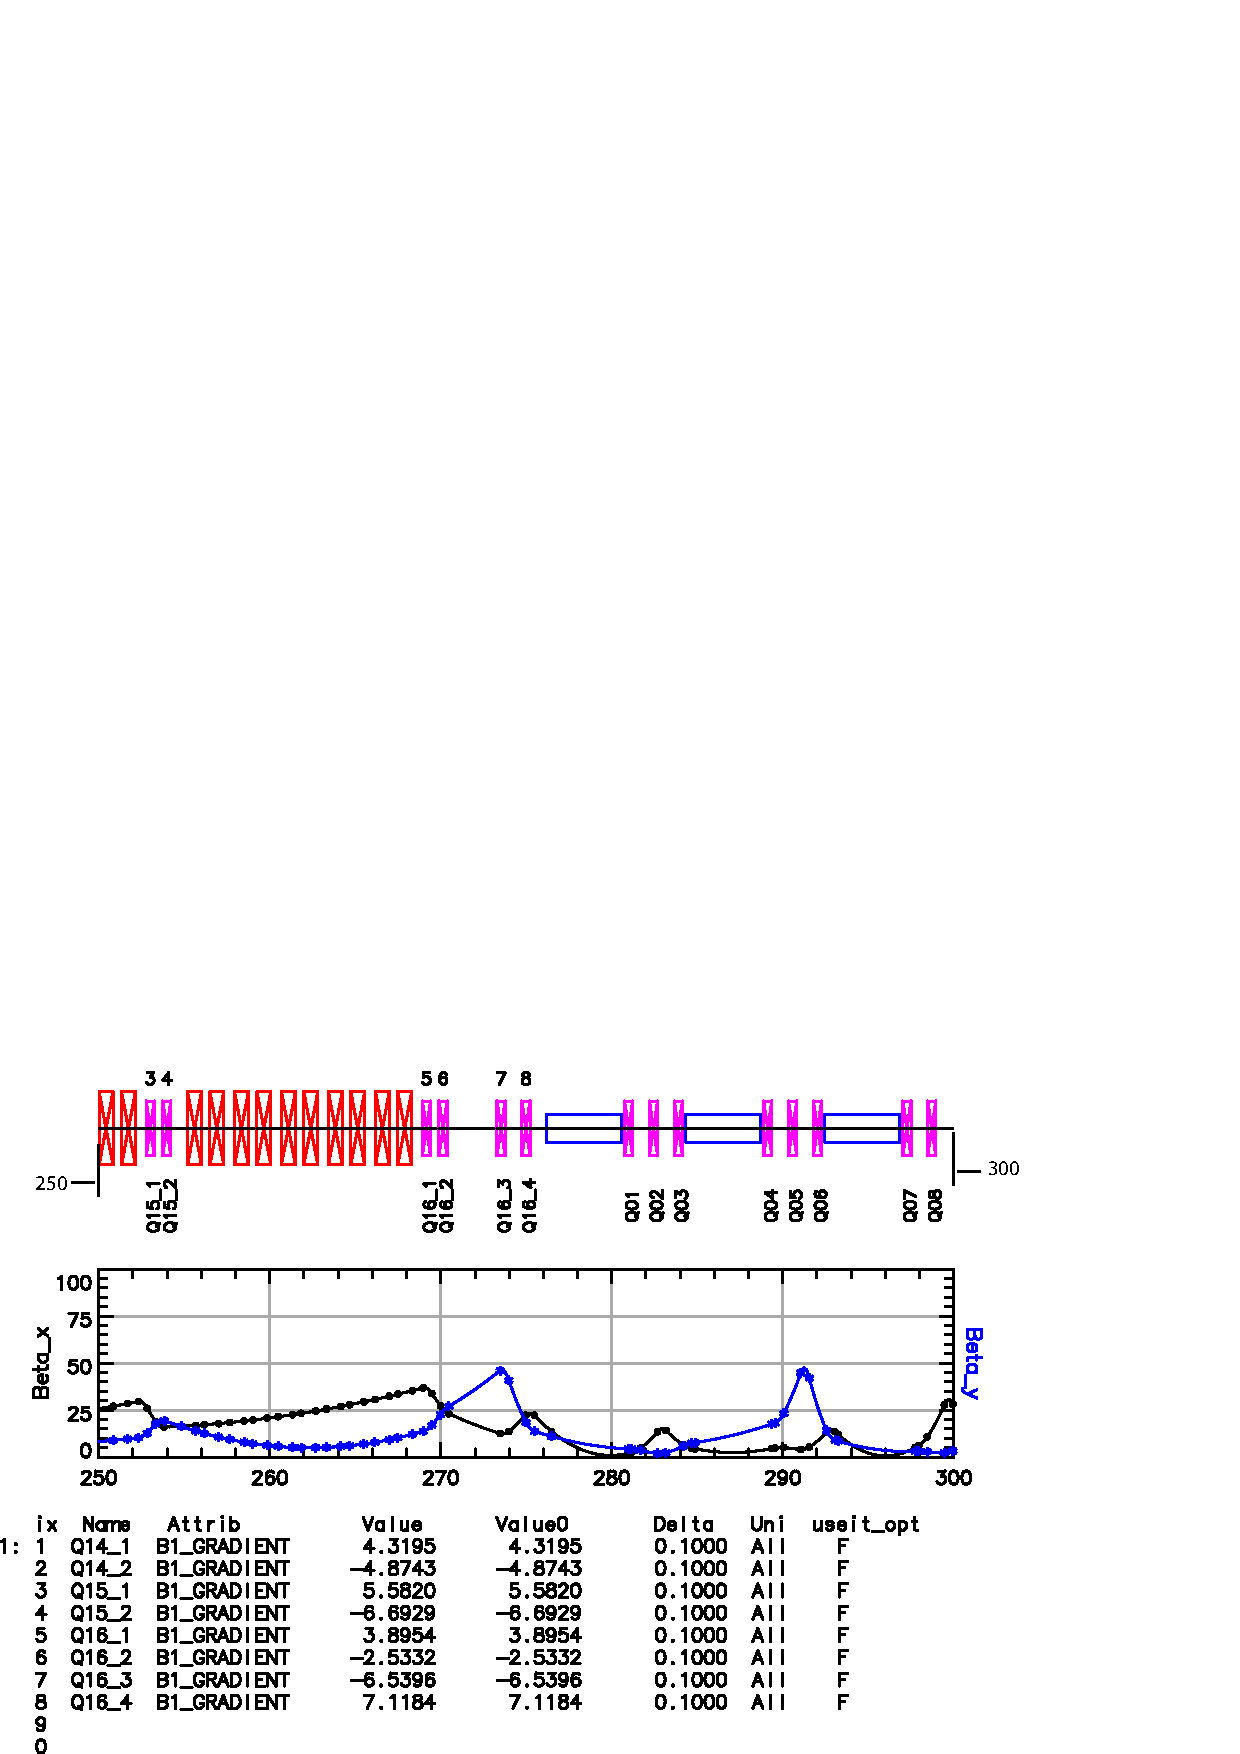
\includegraphics[width=5in]{layout-graph-table.pdf}
  \caption[Example key table with a lattice layout and data plots.]
{A lattice layout plot (top) above a data plot (middle) which in turn is above a key table plot
(bottom). Elements that have attributes that are varied as shown in the key table have the
corresponding key table number printed above the element's glyph in the lattice layout.}
  \label{f:key.table}
\end{figure}

\index{key bindings}
The main purpose of Single Mode is to associate certain keyboard keys with certain variables so that
the pressing of these keys will change their associated model value of the variable as illustrated
in Figure~\ref{f:keyboard}. This is called a \vn{key binding}. Key bindings are established in a
startup file by setting the \vn{var(i)%key_bound} and \vn{var(i)%key_delta} parameters (see
Section~\sref{s:init.var}). After startup, associated variables with keyboard keys can be done using
the \vn{set variable} command (\sref{s:set}).

The variables are divided into banks of 10. The 0\Th bank uses the first ten variables that have
their \vn{key_bound} attribute (\sref{s:init.var}) set to True.  the 1\St bank uses the next ten,
etc.  At any one time, only one bank is active. To see the status of this bank, a \vn{key_table}
plot (\sref{s:key.table})can be setup as shown in Figure~\ref{f:key.table}. The relationship between
the keys and a change in a variable is:
\begin{example}
                 Change by factor of:          
     Variable    -10  -1    1     10
   ----------    ---  ---  ---  -------
    1 + 10*ib     Q    q    1   shift-1   ("!")
    2 + 10*ib     W    w    2   shift-2   ("@")
    3 + 10*ib     E    e    3   shift-3   ("\#")
    4 + 10*ib     R    r    4   shift-4   ("\$")
    5 + 10*ib     T    t    5   shift-5   ("%")
    6 + 10*ib     Y    y    6   shift-6   ("^")
    7 + 10*ib     U    u    7   shift-7   ("\&")
    8 + 10*ib     I    i    8   shift-8   ("*")
    9 + 10*ib     O    o    9   shift-9   ("(")
   10 + 10*ib     P    p    0   shift-0   (")")
\end{example}
In the above table ib is the bank number (0 for the
0\Th bank, etc.), and the change is in multiples of the \vn{step} (\sref{s:init.var}).  value for a
variable. Note: In \vn{line mode}, the command \vn{show key_bindings} (\sref{s:show}) may be used to
show the entire set of bound keys.

Initially the 0\Th bank is active. The left arrow and right arrow are used to decrease or increase
the bank number.  Additionally the "\vn{<}" and "$>$" keys can be used to change the deltas for the
variables.

For example, looking at Figure~\ref{f:key.table}, the \vn{"1:"} in the upper left corner of the
\vn{Key Table} shows that the 1\St bank is active. \vn{key(14)} is associated with the \vn{"4"} key
and from the \vn{Key Table} it is seen that the bound attribute is the \vn{b1_gradient} of the
element named \vn{Q15_2}.  Thus, if the \vn{"4"} key is depressed in single mode, the value of the
\vn{b1_gradient} of element \vn{Q15_2} will be increased by the given Delta (0.1000 in this
case). Pressing the \vn{"r"} key (which is just below the \vn{"4"} key) will decrease the value of
the \vn{b1_gradient} by 0.1000. Using the shift key, which is shift-4 (\vn{"\$"}) will increase
\vn{b1_gradient} by 10 times the given delta (1.000 in this case) and \vn{"R"} will decrease, by a
factor of 10, the given delta.

Since element \vn{Q15_2} is also displayed in the \vn{Lattice Layout}, there is a \vn{"4"} drawn
above this element that reflects the fact that the element contains a bound attribute. Since, in
this case, the Lattice Layout only shows part of the lattice, not all key indexes are present.

%------------------------------------------------------------------------

%% keys ------------------------------------------------------------------------
\section{List of Key Strokes}\index{single mode!list of Key strokes}
\label{s:keys}

In the following list, certain commands use multiple key strokes. For example, the \vn{"/v"} command
is invoked by first pressing the slash (\vn{"/"}) key followed by the \vn{"v"} key. \vn{"a
$<$left_arrow$>$"} represents pressing the \vn{"a"} key followed by the left-arrow key.

Additionally, custom commands can be associated with any key using the \vn{set key} command
\sref{s:set}. Example:
\begin{example}
  set key h = veto var *  ! This sets the "h" key to the command "veto var *"
\end{example}

\begin{description}
\item[?]
Type a short help message.

\item[a $<$left\_arrow$>$]
Pan plots left by half the plot width.

\item[a $<$right\_arrow$>$]
Pan plots right by half the plot width.

\item[a $<$up\_arrow$>$]
Pan plots up by half the plot height.

\item[a $<$down\_arrow$>$]
Pan plots down by half the plot height.

\item[s $<$left\_arrow$>$]
Scale x-axis of plots by a factor of 2.0.

\item[s $<$right\_arrow$>$]
Scale x-axis of plots by a factor of 0.5

\item[s $<$up\_arrow$>$]
Scale y-axis of plots by a factor of 2.0.

\item[s $<$down\_arrow$>$]
Scale y-axis of plots by a factor of 0.5


\item[z $<$left\_arrow$>$]
Zoom x-axis of plots by a factor of 2.0.

\item[z $<$right\_arrow$>$]
Zoom x-axis of plots by a factor of 0.5

\item[z $<$up\_arrow$>$]
Zoom y-axis of plots by a factor of 2.0.

\item[z $<$down\_arrow$>$]
Zoom y-axis of plots by a factor of 0.5

\item[c]  
Show constraints.

\item[g]
Go run the default optimizer (\sref{s:tao.opti}). The optimizer will run until you type a '.' (a
period).  Periodically during the optimization the variable values will be written to files, one for
each universe, whose name is \vn{tao_opt_vars\#.dat}. where \vn{\#} is the universe number.

\item[v]
Show Bmad variable values in bmad lattice format. See also the \vn{/v} command. Equivalent to
\vn{show vars -bmad} in line mode.

\item[V] 
Same an \vn{v} except only variables currently enabled for optimization are shown.
This is equivalent to \vn{show vars -bmad -good} in line mode.

\item[Z] 
Go back to \vn{line mode}

\item[$<$]
Reduce the deltas (the amount that a variable is changed when you use
the keys 0 through 9) of all the variables by a factor of 2.

\item[$>$]
Increase the deltas (the amount that a variable is changed when you
use the keys 0 through 9) of all the variables by a factor of 2.

\item[$<$left\_arrow$>$]
Shift the active key bank down by 1: ib -$>$ ib - 1

\item[$<$right\_arrow$>$]
Shift the active key bank up by 1: ib -$>$ ib + 1

\item[/$<$up\_arrow$>$]
Increase all key deltas by a factor of 10.

\item[/$<$down\_arrow$>$]
Decrease all key deltas by a factor of 10.

\item[$<$CR$>$]
Do nothing but replot.

\item[-p]
Toggle plotting. Whether to plot or not to plot is initially determined by \vn{plot%enable}.

\item['$<$command$>$]
Accept a Line Mode (\sref{c:command}) command.

\item[/b]
Switch the default lattice branch (\sref{s:lattice}).

\item[/e $<$Index or Name$>$]
Prints info on a lattice element. If there are two lattices being used and only the information of
an element from one particular lattice is wanted then prepend with "n@" where n is the lattice
index.

\item[/l]
Print a list of the lattice elements with Twiss parameters.

\item[/u $<$Universe Index$>$]
Switch the default universe (\sref{s:universe}).

\item[/v]
Write variable values to the default output file in Bmad lattice format.  The default output file
name is set by \vn{global%var_out}.  See also the \vn{V} command.

\item[/x $<$min$>$ $<$max$>$]
Set the horizontal scale min and max values for all the plots. This is the same as setting
\vn{default_graph%x%min} and \vn{default_graph%x%max} in the \tao input file. If \vn{min} and
\vn{max} are not given then the scale will be chosen to include the entire lattice.

\item[/y $<$min$>$ $<$max$>$]
Set the y-axis min and max values for all the plots. This is the same as setting \vn{plot%y%min} and
\vn{plot%y%max} in the \tao input file. If \vn{min} and \vn{max} are not given then an autoscale
will be done.

\item[=v $<$digit$>$ $<$value$>$]
Set variable value. \vn{<digit>} is between 0 and 9 corresponding to a
variable of the current bank. \vn{<value>} is the value to set the
variable to.

\item[=$<$right\_arrow$>$]
Set saved ("value0") values to variable values to saved values. The saved values (the value0 column
in the display) are initially set to the initial value on startup. There are saved values for both
the manual and automatic variables. Note that reading in a TOAD input file will reset the saved
values. If you want to save the values of the variables in this case use "/w" to save to a file. Use
the "\vn{/$<$left_arrow$>$}" command to go in the reverse direction.

\item[=$<$left\_arrow$>$]
Paste saved (\vn{value0} column in the display) values back to the variable values.  The saved
values are initially set to the initial value on startup. Use the "\vn{/$<$right_arrow$>$}" command
to go in the reverse direction.

\end{description}


%----------------------------------------------------------------
\part{Programmer's Guide}

\chapter{Python Interface to Tao}
\index{python interface}
\label{c:python}

It is sometimes convenient to interface \tao to a scripting language like Python or interface to
some external program.  Applications include analyzing Tao generated data or 
to interface \tao to an online control system environment.

To aid in interfacing, \tao has the \vn{pipe} command (\sref{s:pipe}).\footnote
  {
Formally this command was called \vn{python} but the name was changed to avoid confusion with
the scripting language Python.
  }
The \vn{pipe} command defaines a standardized syntax with which to communicate with \tao.

Another aid is the \vn{PyTao} package which is an interface layer to be used between \tao and
\vn{Python}. See \sref{s:pytao} for more details.

%--------------------------------------------------------------------------
\section{PyTao Interface}
\label{s:pytao}

The \vn{PyTao} package is an interface layer to be used between \tao and
\vn{Python}. \vn{PyTao} is hosted on \vn{GitHub}
(independent of \bmad distributions) at:
\vspace{-2ex}
\begin{itemize}
  \item[] \url{https://bmad-sim.github.io/pytao}
\end{itemize}
\vspace{-2ex}
Documentation for setup and using PyTao is at:
\begin{example}
  bmad-sim.github.io/pytao/
\end{example}
See the \vn{PyTao} documentation for installation instructions, examples, etc. In this chapter, some
simple examples will be given.

The \vn{PyTao} package uses \tao's \vn{pipe} command to ease integration with \vn{Python}.

There are two ways to interface with Python/PyTao. One way is using the Python \vn{ctypes}
library. The other way is using the \vn{pexpect} module. A Web search will point to documentation on
\vn{ctypes} and \vn{pexpect}. 

\vn{ctypes} is a foreign function library for Python which can be used to link to a \tao shared
library.  The \vn{pexpect} module is a general purpose tool for interfacing Python with programs
like \tao. If \vn{pexpect} is not present your system, it can be downloaded from
\vn{www.noah.org/wiki/pexpect}.

The advantage of \vn{ctypes} is that it directly accesses \tao code
which makes communication between Python and \tao more robust. The disadvantage of \vn{ctypes} is
that it needs a shared-object version of the \vn{Tao} library. [See the Bmad web site for
information on building shared-object libraries.] The disadvantage of \vn{pexpect} is that it is
slower and it is possible for \vn{pexpect} to time out waiting for a response from \tao.

%--------------------------------------------------------------------------
\subsection{Python/PyTao Via Pexpect}

For communicaiton via \vn{pexpect} (\sref{s:pytao}), the python module \vn{tao_pipe.py}, is
provided by \vn{PyTao} in the directory \vn{pytao/tao_pexpect}.

Example Python session:
\begin{example}
  >>> from pytao.tao_pexpect import tao_pipe  # import module
  >>> p = tao_pipe.tao_io("-lat my_lat.bmad") # init session
  >>> out = p.cmd_in("show global")           # Command to Tao
  >>> print(out)                              # print the output from Tao
  >>> p.cmd("show global")                    # Like p.cmd_in() excepts prints the output too.
\end{example}

%--------------------------------------------------------------------------
\subsection{Python/PyTao Interface Via Ctypes}

A \vn{ctypes} based Python module \vn{pytao.py} for interfacing \tao to \vn{Python} is provided by
\vn{PyTao} (\sref{s:pytao}) in the directory \vn{pytao/tao_pexpect}.

A test driver script named \vn{pytao_example.py} is in the same directory. See the documentation in
both of these files for further information.

%--------------------------------------------------------------------------
\section{Tao's Pipe Command}
\label{s:pipe}

\tao's \vn{pipe} (\sref{s:pipe}) command was developed to:
%
\begin{itemize}
\item 
Standardize output of information (data, parameters, etc.) from \tao to simplify the task of
interfacing \tao to external programs especially scripting languages like \vn{Python}.
% 
\item 
Act as an intermediate layer for the control of \tao by such things as machine online control
programs or the planned graphical user interface for \tao.
\end{itemize}

Using the \vn{pipe} command to control \tao will not be covered here. The interested reader is
invited to read the sections of this manual on the coding of \tao and look at the \tao code itself
(which is heavily documented).

Using the \vn{pipe} command is far superior to using the \vn{show} command when interfacing to an
external program. For one, the \vn{pipe} command is formatted for ease of parsing. Another reason
to use the \vn{pipe} command is that, as \tao is developed over time, the output format of the
\vn{pipe} command is much more stable than output from the \vn{show} command.\footnote
  {
The output of the \vn{pipe} command will change when \tao's or \bmad's internal structures are
modified. This is in contrast to the \vn{show} command whose output is formated to be human readible
and whose output format may change on a whim.
  }
Thus the risk of User developed interface code breaking is much reduced by using the \vn{pipe} command.

The general form of the \vn{pipe} command is:
\begin{example}
  pipe <subcommand> <arguments>
\end{example}
The \vn{pipe} command has a number of \vn{subcommands} (over 100) that are listed in
\Sref{s:pipe.sub}. The sub-commands can be divided into two categories. One category are the
``\vn{action}'' subcommands which allow the user to control \tao (for example, creating variables
and data for use in an optimization). The other category are the ``\vn{output}'' subcommands which
output information from \tao.

The output of the \vn{pipe} command are semi-colon delimited lists. Example: With the
\vn{pipe global} the output looks like:
\begin{example}
  lm_opt_deriv_reinit;REAL;T; -1.0000000000000000E+00
  de_lm_step_ratio;REAL;T;  1.0000000000000000E+00
  de_var_to_population_factor;REAL;T;  5.0000000000000000E+00
  unstable_penalty;REAL;T;  1.0000000474974513E-03
  n_opti_cycles;INT;T;20
  track_type;ENUM;T;single
  derivative_uses_design;LOGIC;T;F
  ... etc ...
\end{example}

Most \vn{output} subcommands use ``\vn{parameter list form}'' format where each line has four fields
separated by semicolons:
\begin{example}
  {name};{type};{variable};{value(s)}
\end{example}
The fields are:
\begin{example}
    name:       The name of the parameter

    type:       The type of the parameter:
        INT           Integer number
        REAL          Real number
        COMPLEX       Complex number. A complex number is output as Re;Im
        REAL_ARR      Real array
        LOGIC         Logical: "T" or "F".
        INUM          Integer whose allowed values can be obtained 
                        using the "pipe inum" command.
        ENUM          String whose allowed values can be obtained 
                        using the "pipe enum" command.
        FILE          Name of file.
        CRYSTAL       Crystal name string. EG: "Si(111)"
        DAT_TYPE      Data type string. EG: "orbit.x"
        DAT_TYPE_Z    Data type string if plot%x_axis_type = 'data'. 
                        Otherwise is a data_type_z enum.
        SPECIES       Species name string. EG: "H2SO4++"
        ELE_PARAM     Lattice element parameter string. EG "K1"
        STR           String that does not fall into one of the above string categories.
        STRUCT        Structure. In this case {component_value(s)} is of the form:
                        {name1};{type1};{value1};{name2};{type2};{value2};...
        COMPONENT     For curve component parameters.

    can_vary:   Either 'T', 'F', or 'I', indicating whether or not the
                user may change the value of the parameter. 'I' indicates
                that the parameter is to be ignored by a GUI when displaying parameters.

    value(s):   The value or values of the the parameter. If a parameter has multiple
                values (EG an array), the values will be separated by semicolons.
\end{example}

%--------------------------------------------------------------------------
\section{Plotting Issues}
\label{s:gui.plot}

When using \tao with a \vn{GUI}, and when the \vn{GUI} is doing the plotting, the \vn{-noplot} and
\vn{-external_plotting} options (\sref{s:command.line}) should be used when starting \tao. The
\vn{-noplot} option (which sets \vn{global%plot_on}) prevents \tao from opening a plotting
window. Note: Both of these options can also be set, after startup, with the \vn{set global} command
and the setting of both can be viewed using the \vn{show global} command.

With \vn{-external_plotting} set, the external code should handle how plots are assigned to plot
regions and it would be potentially disruptive if a user tired to place plots (which could
inadvertently happen when running command files). To avoid this, with \vn{-external_plotting} set,
the \vn{place} command will not do any placement but rather save the \vn{place} arguments (which is
the name of a template plot and a region name) to a buffer which then can be read out by the
external code using the \vn{pipe place_buffer} command. The external code may then decide how to
proceed. The external code is able to bypass the buffering and perform placements by using
\vn{place} with the \vn{-no_buffer} switch (\sref{s:place}). Notice: \tao never processes place
command information put in the buffer. It is up to the external code to decide on a course of action.

Normally when \tao is not displaying the plot page when the \vn{-noplot} option is used, \tao will,
to save time, not calculate the points needed for plotting curves. The exception is if
\vn{-external_plotting} is turned on. In this case, to make plot references unambiguous, plot can be
referred to by their index number. The plot index number can be viewed using the \vn{pipe
plot_list} command. Template plots can be referenced using the syntax ``\vn{@Tnnn}'' where \vn{nnn}
is the index number. For example, \vn{@T3} referrers to the template plot with index 3. Similarly,
the displayed plots (plots that are associated with plot regions) can be referred to using the
syntax ``\vn{@Rnnn}''.

%--------------------------------------------------------------------------
\section{Pipe subcommands}
\label{s:pipe.sub}

The \vn{pipe} command has the following subcommands:

% WARNING: this is automatically generated. DO NOT EDIT.

%% pipe beam ------------------------------------
\subsection{pipe beam}
\index{pipe!beam}
\label{p:beam}


Output beam parameters that are not in the beam_init structure.

\begin{example}
   pipe beam \{ix_uni\}@\{ix_branch\}
\end{example}
\begin{verbatim}
Where:
  {ix_uni} is a universe index. Defaults to s%global%default_universe.
  {ix_branch} is a lattice branch index. Defaults to s%global%default_branch.

Note: To set beam_init parameters use the "set beam" command.
\end{verbatim}

%% pipe beam_init ------------------------------------
\subsection{pipe beam_init}
\index{pipe!beam_init}
\label{p:beam.init}


Output beam_init parameters.

\begin{example}
   pipe beam_init \{ix_uni\}@\{ix_branch\}
\end{example}
\begin{verbatim}
Where:
  {ix_uni} is a universe index. Defaults to s%global%default_universe.
  {ix_branch} is a lattice branch index. Defaults to s%global%default_branch.

Note: To set beam_init parameters use the "set beam_init" command
\end{verbatim}

%% pipe bmad_com ------------------------------------
\subsection{pipe bmad_com}
\index{pipe!bmad_com}
\label{p:bmad.com}


Output bmad_com structure components.

\begin{example}
   pipe bmad_com
\end{example}
\begin{verbatim}

\end{verbatim}

%% pipe branch1 ------------------------------------
\subsection{pipe branch1}
\index{pipe!branch1}
\label{p:branch1}


Output lattice branch information for a particular lattice branch.

\begin{example}
   pipe branch1 \{ix_uni\}@\{ix_branch\}
\end{example}
\begin{verbatim}
Where:
  {ix_uni} is a universe index. Defaults to s%global%default_universe.
  {ix_branch} is a lattice branch index. Defaults to s%global%default_branch.
\end{verbatim}

%% pipe bunch_comb ------------------------------------
\subsection{pipe bunch_comb}
\index{pipe!bunch_comb}
\label{p:bunch.comb}


Outputs bunch parameters at a comb point. 
Also see the "write bunch_comb" and "show bunch -comb" commands.

\begin{example}
   pipe bunch_comb \{flags\} \{who\} \{ix_uni\}@\{ix_branch\} \{ix_bunch\}
\end{example}
\begin{verbatim}
Where:
  {flags} are optional switches:
      -array_out : If present, the output will be available in the 
             tao_c_interface_com%c_real array.
  {ix_uni} is a universe index. Defaults to s%global%default_universe.
  {ix_branch} is a branch index. Defaults to s%global%default_branch.
  {ix_bunch} is the bunch index. Defaults to 1.
  {who} is one of:
      x, px, y, py, z, pz, t, s, spin.x, spin.y, spin.z, p0c, beta     -- centroid 
      x.Q, y.Q, z.Q, a.Q, b.Q, c.Q where Q is one of: beta, alpha, gamma, phi, 
                                      eta, etap, sigma, sigma_p, emit, norm_emit
    sigma.IJ where I, J in range [1,6]
    rel_min.I, rel_max.I where I in range [1,6]
    charge_live, n_particle_live, n_particle_lost_in_ele, ix_ele

  Note: If ix_uni or ix_branch is present, "@" must be present.

Example:
  pipe bunch_comb py 2@1 1
\end{verbatim}

%% pipe bunch_params ------------------------------------
\subsection{pipe bunch_params}
\index{pipe!bunch_params}
\label{p:bunch.params}


Outputs bunch parameters at the exit end of a given lattice element.

\begin{example}
   pipe bunch_params \{ele_id\}|\{which\}
\end{example}
\begin{verbatim}
Where:
  {ele_id} is an element name or index.
  {which} is one of: "model", "base" or "design"

Example:
  pipe bunch_params end|model  ! parameters at model lattice element named "end".
\end{verbatim}

%% pipe bunch1 ------------------------------------
\subsection{pipe bunch1}
\index{pipe!bunch1}
\label{p:bunch1}


Outputs Bunch parameters at the exit end of a given lattice element.

\begin{example}
   pipe bunch1 \{ele_id\}|\{which\} \{ix_bunch\} \{coordinate\}
\end{example}
\begin{verbatim}
Where:
  {ele_id} is an element name or index.
  {which} is one of: "model", "base" or "design"
  {ix_bunch} is the bunch index.
  {coordinate} is one of: x, px, y, py, z, pz, "s", "t", "charge", "p0c", 
                                                                "state", "ix_ele"

For example, if {coordinate} = "px", the phase space px coordinate of each particle
of the bunch is displayed. The "state" of a particle is an integer. 
A value of 1 means alive and any other value means the particle has been lost.
\end{verbatim}

%% pipe building_wall_list ------------------------------------
\subsection{pipe building_wall_list}
\index{pipe!building_wall_list}
\label{p:building.wall.list}


Output List of building wall sections or section points

\begin{example}
   pipe building_wall_list \{ix_section\}
\end{example}
\begin{verbatim}
Where:
  {ix_section} is a building wall section index.

If {ix_section} is not present, a list of building wall sections is given.
If {ix_section} is present, a list of section points is given.
\end{verbatim}

%% pipe building_wall_graph ------------------------------------
\subsection{pipe building_wall_graph}
\index{pipe!building_wall_graph}
\label{p:building.wall.graph}


Output (x, y) points for drawing the building wall for a particular graph.

\begin{example}
   pipe building_wall_graph \{graph\}
\end{example}
\begin{verbatim}
Where:
  {graph} is a plot region graph name.

Note: The graph defines the coordinate system for the (x, y) points.
\end{verbatim}

%% pipe building_wall_point ------------------------------------
\subsection{pipe building_wall_point}
\index{pipe!building_wall_point}
\label{p:building.wall.point}


add or delete a building wall point

\begin{example}
   pipe building_wall_point \{ix_section\}^^\{ix_point\}^^\{z\}^^\{x\}^^\{radius\}^^
                                                               \{z_center\}^^\{x_center\}
\end{example}
\begin{verbatim}
Where:
  {ix_section}    -- Section index.
  {ix_point}      -- Point index. Points of higher indexes will be moved up 
                       if adding a point and down if deleting.
  {z}, etc...     -- See tao_building_wall_point_struct components.
                  -- If {z} is set to "delete" then delete the point.
\end{verbatim}

%% pipe building_wall_section ------------------------------------
\subsection{pipe building_wall_section}
\index{pipe!building_wall_section}
\label{p:building.wall.section}


Add or delete a building wall section

\begin{example}
   pipe building_wall_section \{ix_section\}^^\{sec_name\}^^\{sec_constraint\}
\end{example}
\begin{verbatim}
Where:
  {ix_section}      -- Section index. Sections with higher indexes will be
                         moved up if adding a section and down if deleting.
  {sec_name}        -- Section name.
  {sec_constraint}  -- A section constraint name or "delete". Must be one of:
      delete          -- Delete section. Anything else will add the section.
      none
      left_side
      right_side
\end{verbatim}

%% pipe constraints ------------------------------------
\subsection{pipe constraints}
\index{pipe!constraints}
\label{p:constraints}


Output optimization data and variable parameters that contribute to the merit function.

\begin{example}
   pipe constraints \{who\}
\end{example}
\begin{verbatim}
Where:
  {who} is one of: "data" or "var"

Data constraints output is:
  data name
  constraint type
  evaluation element name
  start element name
  end/reference element name
  measured value
  ref value (only relavent if global%opt_with_ref = T)
  model value
  base value (only relavent if global%opt_with_base = T)
  weight
  merit value
  location where merit is evaluated (if there is a range)
Var constraints output is:
  var name
  Associated varible attribute
  meas value
  ref value (only relavent if global%opt_with_ref = T)
  model value
  base value (only relavent if global%opt_with_base = T)
  weight
  merit value
  dmerit/dvar
\end{verbatim}

%% pipe da_aperture ------------------------------------
\subsection{pipe da_aperture}
\index{pipe!da_aperture}
\label{p:da.aperture}


Output dynamic aperture data

\begin{example}
   pipe da_aperture \{ix_uni\}
\end{example}
\begin{verbatim}
Where:
  {ix_uni} is a universe index. Defaults to s%global%default_universe.
\end{verbatim}

%% pipe da_params ------------------------------------
\subsection{pipe da_params}
\index{pipe!da_params}
\label{p:da.params}


Output dynamic aperture input parameters

\begin{example}
   pipe da_params \{ix_uni\}
\end{example}
\begin{verbatim}
Where:
  {ix_uni} is a universe index. Defaults to s%global%default_universe.
\end{verbatim}

%% pipe data ------------------------------------
\subsection{pipe data}
\index{pipe!data}
\label{p:data}


Output Individual datum parameters.

\begin{example}
   pipe data \{ix_uni\}@\{d2_name\}.\{d1_name\}[\{dat_index\}]
\end{example}
\begin{verbatim}
Where:
  {ix_uni} is a universe index. Defaults to s%global%default_universe.
  {d2_name} is the name of the d2_data structure the datum is in.
  {d1_datum} is the name of the d1_data structure the datum is in.
  {dat_index} is the index of the datum.

Use the "pipe data-d1" command to get detailed info on a specific d1 array.

Example:
  pipe data 1@orbit.x[10]
\end{verbatim}

%% pipe data_d_array ------------------------------------
\subsection{pipe data_d_array}
\index{pipe!data_d_array}
\label{p:data.d.array}


Output list of datums for a given d1_data structure.

\begin{example}
   pipe data_d_array \{ix_uni\}@\{d2_name\}.\{d1_name\}
\end{example}
\begin{verbatim}
Where:
  {ix_uni} is a universe index. Defaults to s%global%default_universe.
  {d2_name} is the name of the containing d2_data structure.
  {d1_name} is the name of the d1_data structure containing the array of datums.

Example:
  pipe data_d_array 1@orbit.x
\end{verbatim}

%% pipe data_d1_array ------------------------------------
\subsection{pipe data_d1_array}
\index{pipe!data_d1_array}
\label{p:data.d1.array}


Output list of d1 arrays for a given data_d2.

\begin{example}
   pipe data_d1_array \{d2_datum\}
\end{example}
\begin{verbatim}
{d2_datum} should be of the form
  {ix_uni}@{d2_datum_name}
\end{verbatim}

%% pipe data_d2 ------------------------------------
\subsection{pipe data_d2}
\index{pipe!data_d2}
\label{p:data.d2}


Output information on a d2_datum.

\begin{example}
   pipe data_d2 \{ix_uni\}@\{d2_name\}
\end{example}
\begin{verbatim}
Where:
  {ix_uni} is a universe index. Defaults to s%global%default_universe.
  {d2_name} is the name of the d2_data structure.
\end{verbatim}

%% pipe data_d2_array ------------------------------------
\subsection{pipe data_d2_array}
\index{pipe!data_d2_array}
\label{p:data.d2.array}


Output data d2 info for a given universe.

\begin{example}
   pipe data_d2_array \{ix_uni\}
\end{example}
\begin{verbatim}
Where:
  {ix_uni} is a universe index. Defaults to s%global%default_universe.

Example:
  pipe data_d2_array 1
\end{verbatim}

%% pipe data_d2_create ------------------------------------
\subsection{pipe data_d2_create}
\index{pipe!data_d2_create}
\label{p:data.d2.create}


Create a d2 data structure along with associated d1 and data arrays.

\begin{example}
   pipe data_d2_create \{ix_uni\}@\{d2_name\}^^\{n_d1_data\}^^\{d_data_arrays_name_min_max\}
\end{example}
\begin{verbatim}
Where:
  {ix_uni} is a universe index. Defaults to s%global%default_universe.
  {d2_name} is the name of the d2_data structure to create.
  {n_d1_data} is the number of associated d1 data structures.
  {d_data_arrays_name_min_max} has the form
    {name1}^^{lower_bound1}^^{upper_bound1}^^....
                                           ^^{nameN}^^{lower_boundN}^^{upper_boundN}
  where {name} is the data array name and 
  {lower_bound} and {upper_bound} are the bounds of the array.

Example:
  pipe data_d2_create 2@orbit^^2^^x^^0^^45^^y^^1^^47
This example creates a d2 data structure called "orbit" with 
two d1 structures called "x" and "y".

The "x" d1 structure has an associated data array with indexes in the range [0, 45].
The "y" d1 structure has an associated data arrray with indexes in the range [1, 47].

Use the "set data" command to set created datum parameters.

Note: When setting multiple data parameters, 
      temporarily toggle s%global%lattice_calc_on to False
  ("set global lattice_calc_on = F") to prevent Tao trying to 
      evaluate the partially created datum and generating unwanted error messages.
\end{verbatim}

%% pipe data_d2_destroy ------------------------------------
\subsection{pipe data_d2_destroy}
\index{pipe!data_d2_destroy}
\label{p:data.d2.destroy}


Destroy a d2 data structure along with associated d1 and data arrays.

\begin{example}
   pipe data_d2_destroy \{ix_uni\}@\{d2_name\}
\end{example}
\begin{verbatim}
Where:
  {ix_uni} is a universe index. Defaults to s%global%default_universe.
  {d2_name} is the name of the d2_data structure to destroy.

Example:
  pipe data_d2_destroy 2@orbit
This destroys the orbit d2_data structure in universe 2.
\end{verbatim}

%% pipe data_parameter ------------------------------------
\subsection{pipe data_parameter}
\index{pipe!data_parameter}
\label{p:data.parameter}


Output an array of values for a particular datum parameter for a given array of datums, 

\begin{example}
   pipe data_parameter \{data_array\} \{parameter\}
\end{example}
\begin{verbatim}
{parameter} may be any tao_data_struct parameter.
Example:
  pipe data_parameter orbit.x model_value
\end{verbatim}

%% pipe data_set_design_value ------------------------------------
\subsection{pipe data_set_design_value}
\index{pipe!data_set_design_value}
\label{p:data.set.design.value}


Set the design (and base \& model) values for all datums.

\begin{example}
   pipe data_set_design_value
\end{example}
\begin{verbatim}
Example:
  pipe data_set_design_value

Note: Use the "data_d2_create" and "datum_create" first to create datums.
\end{verbatim}

%% pipe datum_create ------------------------------------
\subsection{pipe datum_create}
\index{pipe!datum_create}
\label{p:datum.create}


Create a datum.

\begin{example}
   pipe datum_create \{datum_name\}^^\{data_type\}^^\{ele_ref_name\}^^\{ele_start_name\}^^
                       \{ele_name\}^^\{merit_type\}^^\{meas\}^^\{good_meas\}^^\{ref\}^^
                       \{good_ref\}^^\{weight\}^^\{good_user\}^^\{data_source\}^^
                       \{eval_point\}^^\{s_offset\}^^\{ix_bunch\}^^\{invalid_value\}^^
                       \{spin_axis%n0(1)\}^^\{spin_axis%n0(2)\}^^\{spin_axis%n0(3)\}^^
                       \{spin_axis%l(1)\}^^\{spin_axis%l(2)\}^^\{spin_axis%l(3)\}
\end{example}
\begin{verbatim}
Note: The 3 values for spin_axis%n0, as a group, are optional. 
      Also the 3 values for spin_axis%l are, as a group, optional.
Note: Use the "pipe data_d2_create" command first to create a d2 structure 
      with associated d1 arrays.
Note: After creating all your datums, use the "pipe data_set_design_value" routine
      to set the design (and model) values.
\end{verbatim}

%% pipe datum_has_ele ------------------------------------
\subsection{pipe datum_has_ele}
\index{pipe!datum_has_ele}
\label{p:datum.has.ele}


Output whether a datum type has an associated lattice element

\begin{example}
   pipe datum_has_ele \{datum_type\}
\end{example}
\begin{verbatim}

\end{verbatim}

%% pipe derivative ------------------------------------
\subsection{pipe derivative}
\index{pipe!derivative}
\label{p:derivative}


Output optimization derivatives

\begin{example}
   pipe derivative
\end{example}
\begin{verbatim}
Note: To save time, this command will not recalculate derivatives. 
Use the "derivative" command beforehand to recalcuate if needed.
\end{verbatim}

%% pipe ele:ac_kicker ------------------------------------
\subsection{pipe ele:ac_kicker}
\index{pipe!ele:ac_kicker}
\label{p:ele:ac.kicker}


Output element ac_kicker parameters

\begin{example}
   pipe ele:ac_kicker \{ele_id\}|\{which\}
\end{example}
\begin{verbatim}
Where: 
  {ele_id} is an element name or index.
  {which} is one of: "model", "base" or "design"

Example:
  pipe ele:ac_kicker 3@1>>7|model
This gives element number 7 in branch 1 of universe 3.
\end{verbatim}

%% pipe ele:cartesian_map ------------------------------------
\subsection{pipe ele:cartesian_map}
\index{pipe!ele:cartesian_map}
\label{p:ele:cartesian.map}


Output element cartesian_map parameters

\begin{example}
   pipe ele:cartesian_map \{ele_id\}|\{which\} \{index\} \{who\}
\end{example}
\begin{verbatim}
Where:
  {ele_id} is an element name or index
  {which} is one of: "model", "base" or "design"
  {index} is the index number in the ele%cartesian_map(:) array
  {who} is one of: "base", or "terms"

Example:
  pipe ele:cartesian_map 3@1>>7|model 2 base
This gives element number 7 in branch 1 of universe 3.
\end{verbatim}

%% pipe ele:chamber_wall ------------------------------------
\subsection{pipe ele:chamber_wall}
\index{pipe!ele:chamber_wall}
\label{p:ele:chamber.wall}


Output element beam chamber wall parameters

\begin{example}
   pipe ele:chamber_wall \{ele_id\}|\{which\} \{index\} \{who\}
\end{example}
\begin{verbatim}
Where:
  {ele_id} is an element name or index.
  {which} is one of: "model", "base" or "design"
  {index} is index of the wall.
  {who} is one of:
    "x"       ! Return min/max in horizontal plane
    "y"       ! Return min/max in vertical plane
\end{verbatim}

%% pipe ele:control_var ------------------------------------
\subsection{pipe ele:control_var}
\index{pipe!ele:control_var}
\label{p:ele:control.var}


Output list of element control variables.
Used for group, overlay and ramper type elements.

\begin{example}
   pipe ele:control_var \{ele_id\}|\{which\}
\end{example}
\begin{verbatim}
Where:
  {ele_id} is an element name or index.
  {which} is one of: "model", "base" or "design"

Example:
  pipe ele:control_var 3@1>>7|model
This gives control info on element number 7 in branch 1 of universe 3.
\end{verbatim}

%% pipe ele:cylindrical_map ------------------------------------
\subsection{pipe ele:cylindrical_map}
\index{pipe!ele:cylindrical_map}
\label{p:ele:cylindrical.map}


Output element cylindrical_map

\begin{example}
   pipe ele:cylindrical_map \{ele_id\}|\{which\} \{index\} \{who\}
\end{example}
\begin{verbatim}
Where 
  {ele_id} is an element name or index.
  {which} is one of: "model", "base" or "design"
  {index} is the index number in the ele%cylindrical_map(:) array
  {who} is one of: "base", or "terms"

Example:
  pipe ele:cylindrical_map 3@1>>7|model 2 base
This gives map #2 of element number 7 in branch 1 of universe 3.
\end{verbatim}

%% pipe ele:elec_multipoles ------------------------------------
\subsection{pipe ele:elec_multipoles}
\index{pipe!ele:elec_multipoles}
\label{p:ele:elec.multipoles}


Output element electric multipoles

\begin{example}
   pipe ele:elec_multipoles \{ele_id\}|\{which\}
\end{example}
\begin{verbatim}
Where:
  {ele_id} is an element name or index.
  {which} is one of: "model", "base" or "design"

Example:
  pipe ele:elec_multipoles 3@1>>7|model
This gives element number 7 in branch 1 of universe 3.
\end{verbatim}

%% pipe ele:floor ------------------------------------
\subsection{pipe ele:floor}
\index{pipe!ele:floor}
\label{p:ele:floor}


Output element floor coordinates. The output gives four lines. "Reference" is
without element misalignments and "Actual" is with misalignments. The lines with "-W"
give the W matrix. The exception is that if ele is a multipass_lord, there will be 4*N
lines where N is the number of slaves.

\begin{example}
   pipe ele:floor \{ele_id\}|\{which\} \{where\}
\end{example}
\begin{verbatim}
Where:
  {ele_id} is an element name or index.
  {which} is one of: "model", "base" or "design"
  {where} is an optional argument which, if present, is one of
    beginning  ! Upstream end.
    center     ! Middle of the element. This is the surface of element when used 
               !  with photonic reflecting elements such as crystal and mirror elements.
    end        ! Downstream end (default).

Example:
  pipe ele:floor 3@1>>7|model
This gives element number 7 in branch 1 of universe 3.
\end{verbatim}

%% pipe ele:gen_attribs ------------------------------------
\subsection{pipe ele:gen_attribs}
\index{pipe!ele:gen_attribs}
\label{p:ele:gen.attribs}


Output element general attributes

\begin{example}
   pipe ele:gen_attribs \{ele_id\}|\{which\}
\end{example}
\begin{verbatim}
Where: 
  {ele_id} is an element name or index.
  {which} is one of: "model", "base" or "design"

Example:
  pipe ele:gen_attribs 3@1>>7|model
This gives element number 7 in branch 1 of universe 3.
\end{verbatim}

%% pipe ele:gen_grad_map ------------------------------------
\subsection{pipe ele:gen_grad_map}
\index{pipe!ele:gen_grad_map}
\label{p:ele:gen.grad.map}


Output element gen_grad_map 

\begin{example}
   pipe ele:gen_grad_map \{ele_id\}|\{which\} \{index\} \{who\}
\end{example}
\begin{verbatim}
Where: 
  {ele_id} is an element name or index.
  {which} is one of: "model", "base" or "design"
  {index} is the index number in the ele%gen_grad_map(:) array
  {who} is one of: "base", or "derivs".

Example:
  pipe ele:gen_grad_map 3@1>>7|model 2 base
This gives element number 7 in branch 1 of universe 3.
\end{verbatim}

%% pipe ele:grid_field ------------------------------------
\subsection{pipe ele:grid_field}
\index{pipe!ele:grid_field}
\label{p:ele:grid.field}


Output element grid_field

\begin{example}
   pipe ele:grid_field \{ele_id\}|\{which\} \{index\} \{who\}
\end{example}
\begin{verbatim}
Where:
  {ele_id} is an element name or index.
  {which} is one of: "model", "base" or "design"
  {index} is the index number in the ele%grid_field(:) array.
  {who} is one of: "base", or "points"

Example:
  pipe ele:grid_field 3@1>>7|model 2 base
This gives grid #2 of element number 7 in branch 1 of universe 3.
\end{verbatim}

%% pipe ele:head ------------------------------------
\subsection{pipe ele:head}
\index{pipe!ele:head}
\label{p:ele:head}


Output "head" Element attributes

\begin{example}
   pipe ele:head \{ele_id\}|\{which\}
\end{example}
\begin{verbatim}
Where: 
  {ele_id} is an element name or index.
  {which} is one of: "model", "base" or "design"

Example:
  pipe ele:head 3@1>>7|model
This gives element number 7 in branch 1 of universe 3.
\end{verbatim}

%% pipe ele:lord_slave ------------------------------------
\subsection{pipe ele:lord_slave}
\index{pipe!ele:lord_slave}
\label{p:ele:lord.slave}


Output the lord/slave tree of an element.

\begin{example}
   pipe ele:lord_slave \{ele_id\}|\{which\}
\end{example}
\begin{verbatim}
Where: 
  {ele_id} is an element name or index.
  {which} is one of: "model", "base" or "design"

Example:
  pipe ele:lord_slave 3@1>>7|model
This gives lord and slave info on element number 7 in branch 1 of universe 3.
Note: The lord/slave info is independent of the setting of {which}.

The output is a number of lines.
Each line gives information on an element (element index, etc.).
Some lines begin with the word "Element". 
After each "Element" line, there are a number of lines (possibly zero) 
that begin with the word "Slave or "Lord".
These "Slave" and "Lord" lines are the slaves and lords of the "Element" element.
\end{verbatim}

%% pipe ele:mat6 ------------------------------------
\subsection{pipe ele:mat6}
\index{pipe!ele:mat6}
\label{p:ele:mat6}


Output element mat6

\begin{example}
   pipe ele:mat6 \{ele_id\}|\{which\} \{who\}
\end{example}
\begin{verbatim}
Where: 
  {ele_id} is an element name or index.
  {which} is one of: "model", "base" or "design"
  {who} is one of: "mat6", "vec0", or "err"

Example:
  pipe ele:mat6 3@1>>7|model mat6
This gives element number 7 in branch 1 of universe 3.
\end{verbatim}

%% pipe ele:methods ------------------------------------
\subsection{pipe ele:methods}
\index{pipe!ele:methods}
\label{p:ele:methods}


Output element methods

\begin{example}
   pipe ele:methods \{ele_id\}|\{which\}
\end{example}
\begin{verbatim}
Where: 
  {ele_id} is an element name or index.
  {which} is one of: "model", "base" or "design"

Example:
  pipe ele:methods 3@1>>7|model
This gives element number 7 in branch 1 of universe 3.
\end{verbatim}

%% pipe ele:multipoles ------------------------------------
\subsection{pipe ele:multipoles}
\index{pipe!ele:multipoles}
\label{p:ele:multipoles}


Output element multipoles

\begin{example}
   pipe ele:multipoles \{ele_id\}|\{which\}
\end{example}
\begin{verbatim}
Where: 
  {ele_id} is an element name or index.
  {which} is one of: "model", "base" or "design"

Example:
  pipe ele:multipoles 3@1>>7|model
This gives element number 7 in branch 1 of universe 3.
\end{verbatim}

%% pipe ele:orbit ------------------------------------
\subsection{pipe ele:orbit}
\index{pipe!ele:orbit}
\label{p:ele:orbit}


Output element orbit

\begin{example}
   pipe ele:orbit \{ele_id\}|\{which\}
\end{example}
\begin{verbatim}
Where: 
  {ele_id} is an element name or index.
  {which} is one of: "model", "base" or "design"

Example:
  pipe ele:orbit 3@1>>7|model
This gives element number 7 in branch 1 of universe 3.
\end{verbatim}

%% pipe ele:param ------------------------------------
\subsection{pipe ele:param}
\index{pipe!ele:param}
\label{p:ele:param}


Output lattice element parameter

\begin{example}
   pipe ele:param \{ele_id\}|\{which\} \{who\}
\end{example}
\begin{verbatim}
Where: 
  {ele_id} is an element name or index.
  {which} is one of: "model", "base" or "design"
  {who} values are the same as {who} values for "pipe lat_list".
        Note: Here {who} must be a single parameter and not a list.

Example:
  pipe ele:param 3@1>>7|model e_tot
This gives E_tot of element number 7 in branch 1 of universe 3.

Note: On output the {variable} component will always be "F" (since this 
command cannot tell if a parameter is allowed to vary).

Also see: "pipe lat_list".
\end{verbatim}

%% pipe ele:photon ------------------------------------
\subsection{pipe ele:photon}
\index{pipe!ele:photon}
\label{p:ele:photon}


Output element photon parameters

\begin{example}
   pipe ele:photon \{ele_id\}|\{which\} \{who\}
\end{example}
\begin{verbatim}
Where: 
  {ele_id} is an element name or index.
  {which} is one of: "model", "base" or "design"
  {who} is one of: "base", "material", or "curvature"

Example:
  pipe ele:photon 3@1>>7|model base
This gives element number 7 in branch 1 of universe 3.
\end{verbatim}

%% pipe ele:spin_taylor ------------------------------------
\subsection{pipe ele:spin_taylor}
\index{pipe!ele:spin_taylor}
\label{p:ele:spin.taylor}


Output element spin_taylor parameters

\begin{example}
   pipe ele:spin_taylor \{ele_id\}|\{which\}
\end{example}
\begin{verbatim}
Where: 
  {ele_id} is an element name or index.
  {which} is one of: "model", "base" or "design"

Example:
  pipe ele:spin_taylor 3@1>>7|model
This gives element number 7 in branch 1 of universe 3.
\end{verbatim}

%% pipe ele:taylor ------------------------------------
\subsection{pipe ele:taylor}
\index{pipe!ele:taylor}
\label{p:ele:taylor}


Output element taylor map 

\begin{example}
   pipe ele:taylor \{ele_id\}|\{which\}
\end{example}
\begin{verbatim}
Where: 
  {ele_id} is an element name or index.
  {which} is one of: "model", "base" or "design"

Example:
  pipe ele:taylor 3@1>>7|model
This gives element number 7 in branch 1 of universe 3.
\end{verbatim}

%% pipe ele:twiss ------------------------------------
\subsection{pipe ele:twiss}
\index{pipe!ele:twiss}
\label{p:ele:twiss}


Output element Twiss parameters

\begin{example}
   pipe ele:twiss \{ele_id\}|\{which\}
\end{example}
\begin{verbatim}
Where: 
  {ele_id} is an element name or index.
  {which} is one of: "model", "base" or "design"

Example:
  pipe ele:twiss 3@1>>7|model
This gives element number 7 in branch 1 of universe 3.
\end{verbatim}

%% pipe ele:wake ------------------------------------
\subsection{pipe ele:wake}
\index{pipe!ele:wake}
\label{p:ele:wake}


Output element wake.

\begin{example}
   pipe ele:wake \{ele_id\}|\{which\} \{who\}
\end{example}
\begin{verbatim}
Where: 
  {ele_id} is an element name or index.
  {which} is one of: "model", "base" or "design"
  {Who} is one of:
      "sr_long"        "sr_long_table"
      "sr_trans"       "sr_trans_table"
      "lr_mode_table"  "base"

Example:
  pipe ele:wake 3@1>>7|model
This gives element number 7 in branch 1 of universe 3.
\end{verbatim}

%% pipe ele:wall3d ------------------------------------
\subsection{pipe ele:wall3d}
\index{pipe!ele:wall3d}
\label{p:ele:wall3d}


Output element wall3d parameters.

\begin{example}
   pipe ele:wall3d \{ele_id\}|\{which\} \{index\} \{who\}
\end{example}
\begin{verbatim}
Where: 
  {ele_id} is an element name or index.
  {which} is one of: "model", "base" or "design"
  {index} is the index number in the ele%wall3d(:) array 
            The size of this array is obtained from "pipe ele:head".
  {who} is one of: "base", or "table".
Example:
  pipe ele:wall3d 3@1>>7|model 2 base
This gives element number 7 in branch 1 of universe 3.
\end{verbatim}

%% pipe evaluate ------------------------------------
\subsection{pipe evaluate}
\index{pipe!evaluate}
\label{p:evaluate}


Output the value of an expression. The result may be a vector.

\begin{example}
   pipe evaluate \{flags\} \{expression\}
\end{example}
\begin{verbatim}
Where:
  Optional {flags} are:
      -array_out : If present, the output will be available in the 
                    tao_c_interface_com%c_real array.
  {expression} is expression to be evaluated.

Example:
  pipe evaluate 3+data::cbar.11[1:10]|model
\end{verbatim}

%% pipe em_field ------------------------------------
\subsection{pipe em_field}
\index{pipe!em_field}
\label{p:em.field}


Output EM field at a given point generated by a given element.

\begin{example}
   pipe em_field \{ele_id\}|\{which\} \{x\} \{y\} \{z\} \{t_or_z\}
\end{example}
\begin{verbatim}
Where:
  {which} is one of: "model", "base" or "design"
  {x}, {y}  -- Transverse coords.
  {z}       -- Longitudinal coord with respect to entrance end of element.
  {t_or_z}  -- time or phase space z depending if lattice is setup for 
            --   absolute time tracking.
\end{verbatim}

%% pipe enum ------------------------------------
\subsection{pipe enum}
\index{pipe!enum}
\label{p:enum}


Output list of possible values for enumerated numbers.

\begin{example}
   pipe enum \{enum_name\}
\end{example}
\begin{verbatim}
Example:
  pipe enum tracking_method
\end{verbatim}

%% pipe floor_plan ------------------------------------
\subsection{pipe floor_plan}
\index{pipe!floor_plan}
\label{p:floor.plan}


Output (x,y) points and other information that can be used for drawing a floor_plan.

\begin{example}
   pipe floor_plan \{graph\}
\end{example}
\begin{verbatim}

\end{verbatim}

%% pipe floor_orbit ------------------------------------
\subsection{pipe floor_orbit}
\index{pipe!floor_orbit}
\label{p:floor.orbit}


Output (x, y) coordinates for drawing the particle orbit on a floor plan.

\begin{example}
   pipe floor_orbit \{graph\}
\end{example}
\begin{verbatim}

\end{verbatim}

%% pipe global ------------------------------------
\subsection{pipe global}
\index{pipe!global}
\label{p:global}


Output global parameters.

\begin{example}
   pipe global
\end{example}
\begin{verbatim}
Output syntax is parameter list form. See documentation at the beginning of this file.

Note: The follow is intentionally left out:
  optimizer_allow_user_abort
  quiet
  single_step
  prompt_color
  prompt_string
\end{verbatim}

%% pipe global:optimization ------------------------------------
\subsection{pipe global:optimization}
\index{pipe!global:optimization}
\label{p:global:optimization}


Output optimization parameters.
Also see global:opti_de.

\begin{example}
   pipe global:optimization
\end{example}
\begin{verbatim}
Output syntax is parameter list form. See documentation at the beginning of this file.
\end{verbatim}

%% pipe global:opti_de ------------------------------------
\subsection{pipe global:opti_de}
\index{pipe!global:opti_de}
\label{p:global:opti.de}


Output DE optimization parameters.

\begin{example}
   pipe global:opti_de
\end{example}
\begin{verbatim}
Output syntax is parameter list form. See documentation at the beginning of this file.
\end{verbatim}

%% pipe help ------------------------------------
\subsection{pipe help}
\index{pipe!help}
\label{p:help}


Output list of "help xxx" topics

\begin{example}
   pipe help
\end{example}
\begin{verbatim}

\end{verbatim}

%% pipe inum ------------------------------------
\subsection{pipe inum}
\index{pipe!inum}
\label{p:inum}


Output list of possible values for an INUM parameter.
For example, possible index numbers for the branches of a lattice.

\begin{example}
   pipe inum \{who\}
\end{example}
\begin{verbatim}

\end{verbatim}

%% pipe lat_calc_done ------------------------------------
\subsection{pipe lat_calc_done}
\index{pipe!lat_calc_done}
\label{p:lat.calc.done}


Output if a lattice recalculation has been proformed since the last 
  time "pipe lat_calc_done" was called.

\begin{example}
   pipe lat_calc_done
\end{example}
\begin{verbatim}

\end{verbatim}

%% pipe lat_ele_list ------------------------------------
\subsection{pipe lat_ele_list}
\index{pipe!lat_ele_list}
\label{p:lat.ele.list}


Output lattice element list.

\begin{example}
   pipe lat_ele_list \{branch_name\}
\end{example}
\begin{verbatim}
{branch_name} should have the form:
  {ix_uni}@{ix_branch}
\end{verbatim}

%% pipe lat_header ------------------------------------
\subsection{pipe lat_header}
\index{pipe!lat_header}
\label{p:lat.header}


Output lattice "header" info like the lattice and machine names.

\begin{example}
   pipe lat_header \{ix_uni\}
\end{example}
\begin{verbatim}
Output syntax is parameter list form. See documentation at the beginning of this file.
\end{verbatim}

%% pipe lat_branch_list ------------------------------------
\subsection{pipe lat_branch_list}
\index{pipe!lat_branch_list}
\label{p:lat.branch.list}


Output lattice branch list

\begin{example}
   pipe lat_branch_list \{ix_uni\}
\end{example}
\begin{verbatim}
Output syntax:
  branch_index;branch_name;n_ele_track;n_ele_max
\end{verbatim}

%% pipe lat_list ------------------------------------
\subsection{pipe lat_list}
\index{pipe!lat_list}
\label{p:lat.list}


Output list of parameters at ends of lattice elements

\begin{example}
   pipe lat_list \{flags\} \{ix_uni\}@\{ix_branch\}>>\{elements\}|\{which\} \{who\}
\end{example}
\begin{verbatim}
Where:
 Optional {flags} are:
  -no_slaves   - If present, multipass_slave and super_slave elements will not 
               -   be matched to.
  -track_only  - If present, lord elements will not be matched to.
  -index_order - If present, order elements by element index instead of the 
               -   standard s-position.
  -array_out   - If present, the output will be available in the 
    tao_c_interface_com%c_real or tao_c_interface_com%c_integer arrays. 
    See the code below for when %c_real vs %c_integer is used.
    Note: Only a single {who} item permitted when -array_out is present.

  {which} is one of: "model", "base" or "design"

  {who} is a comma deliminated list of:
    orbit.floor.x, orbit.floor.y, orbit.floor.z    ! Floor coords at particle orbit.
    orbit.spin.1, orbit.spin.2, orbit.spin.3,
    orbit.vec.1, orbit.vec.2, orbit.vec.3, orbit.vec.4, orbit.vec.5, orbit.vec.6,
    orbit.t, orbit.beta,
    orbit.state,     ! Note: state is an integer. alive$ = 1, anything else is lost.
    orbit.energy, orbit.pc,
    ele.name, ele.key, ele.ix_ele, ele.ix_branch
    ele.a.beta, ele.a.alpha, ele.a.eta, ele.a.etap, ele.a.gamma, ele.a.phi,
    ele.b.beta, ele.b.alpha, ele.b.eta, ele.b.etap, ele.b.gamma, ele.b.phi,
    ele.x.eta, ele.x.etap,
    ele.y.eta, ele.y.etap,
    ele.ref_time, ele.ref_time_start
    ele.s, ele.l
    ele.e_tot, ele.p0c
    ele.mat6      ! Output: mat6(1,:), mat6(2,:), ... mat6(6,:)
    ele.vec0      ! Output: vec0(1), ... vec0(6)
    ele.c_mat     ! Output: c_mat11, c_mat12, c_mat21, c_mat22.
    ele.gamma_c   ! Parameter associated with coupling c-matrix.
    ele.XXX       ! Where XXX is a Bmad syntax element attribute. 
                  !   EG: ele.beta_a, ele.k1, etc.

  {elements} is a string to match element names to.
    Use "*" to match to all elements.

Examples:
  pipe lat_list -track 3@0>>Q*|base ele.s,orbit.vec.2
  pipe lat_list 3@0>>Q*|base real:ele.s    

Also see: "pipe ele:param"
\end{verbatim}

%% pipe lat_param_units ------------------------------------
\subsection{pipe lat_param_units}
\index{pipe!lat_param_units}
\label{p:lat.param.units}


Output units of a parameter associated with a lattice or lattice element.

\begin{example}
   pipe lat_param_units \{param_name\}
\end{example}
\begin{verbatim}

\end{verbatim}

%% pipe matrix ------------------------------------
\subsection{pipe matrix}
\index{pipe!matrix}
\label{p:matrix}


Output matrix value from the exit end of one element to the exit end of the other.

\begin{example}
   pipe matrix \{ele1_id\} \{ele2_id\}
\end{example}
\begin{verbatim}
Where:
  {ele1_id} is the start element.
  {ele2_id} is the end element.
If {ele2_id} = {ele1_id}, the 1-turn transfer map is computed.
Note: {ele2_id} should just be an element name or index without universe, 
      branch, or model/base/design specification.

Example:
  pipe matrix 2@1>>q01w|design q02w
\end{verbatim}

%% pipe merit ------------------------------------
\subsection{pipe merit}
\index{pipe!merit}
\label{p:merit}


Output merit value.

\begin{example}
   pipe merit
\end{example}
\begin{verbatim}

\end{verbatim}

%% pipe orbit_at_s ------------------------------------
\subsection{pipe orbit_at_s}
\index{pipe!orbit_at_s}
\label{p:orbit.at.s}


Output twiss at given s position.

\begin{example}
   pipe orbit_at_s \{ix_uni\}@\{ele\}->\{s_offset\}|\{which\}
\end{example}
\begin{verbatim}
Where:
  {ix_uni}   - Universe index. Defaults to s%global%default_universe.
  {ele}      - Element name or index. 
                 Default at the Beginning element at start of branch 0.
  {s_offset} - Offset of the evaluation point from the downstream end of ele. 
                 Default is 0. If {s_offset} is present, the preceeding "->" sign
                 must be present. EG: Something like "23|model" will {which} is 
                 one of: "model", "base" or "design".

Example:
  pipe orbit_at_s Q10->0.4|model   ! Orbit at 0.4 meters from Q10 element exit end in model lattice.
\end{verbatim}

%% pipe place_buffer ------------------------------------
\subsection{pipe place_buffer}
\index{pipe!place_buffer}
\label{p:place.buffer}


Output the place command buffer and reset the buffer.
The contents of the buffer are the place commands that the user has issued.
See the Tao manual for more details.

\begin{example}
   pipe place_buffer
\end{example}
\begin{verbatim}

\end{verbatim}

%% pipe plot_curve ------------------------------------
\subsection{pipe plot_curve}
\index{pipe!plot_curve}
\label{p:plot.curve}


Output curve information for a plot.

\begin{example}
   pipe plot_curve \{curve_name\}
\end{example}
\begin{verbatim}

\end{verbatim}

%% pipe plot_graph ------------------------------------
\subsection{pipe plot_graph}
\index{pipe!plot_graph}
\label{p:plot.graph}


Output graph info.

\begin{example}
   pipe plot_graph \{graph_name\}
\end{example}
\begin{verbatim}
{graph_name} is in the form:
  {p_name}.{g_name}
where
  {p_name} is the plot region name if from a region or the plot name if a template plot.
  This name is obtained from the pipe plot_list command.
  {g_name} is the graph name obtained from the pipe plot1 command.
\end{verbatim}

%% pipe plot_histogram ------------------------------------
\subsection{pipe plot_histogram}
\index{pipe!plot_histogram}
\label{p:plot.histogram}


Output plot histogram info.

\begin{example}
   pipe plot_histogram \{curve_name\}
\end{example}
\begin{verbatim}

\end{verbatim}

%% pipe plot_lat_layout ------------------------------------
\subsection{pipe plot_lat_layout}
\index{pipe!plot_lat_layout}
\label{p:plot.lat.layout}


Output plot Lat_layout info

\begin{example}
   pipe plot_lat_layout \{ix_uni\}@\{ix_branch\}
\end{example}
\begin{verbatim}
Note: The returned list of element positions is not ordered in increasing
      longitudinal position.
\end{verbatim}

%% pipe plot_list ------------------------------------
\subsection{pipe plot_list}
\index{pipe!plot_list}
\label{p:plot.list}


Output list of plot templates or plot regions.

\begin{example}
   pipe plot_list \{r_or_g\}
\end{example}
\begin{verbatim}
where "{r/g}" is:
  "r"      ! list regions of the form ix;region_name;plot_name;visible;x1;x2;y1;y2
  "t"      ! list template plots of the form ix;name
\end{verbatim}

%% pipe plot_template_manage ------------------------------------
\subsection{pipe plot_template_manage}
\index{pipe!plot_template_manage}
\label{p:plot.template.manage}


Template plot creation or destruction.

\begin{example}
   pipe plot_template_manage \{template_location\}^^\{template_name\}^^
                          \{n_graph\}^^\{graph_names\}
\end{example}
\begin{verbatim}
Where:
  {template_location} - Location to place or delete a template plot. 
                          Use "@Tnnn" syntax for the location.
  {template_name}     - The name of the template plot. 
                          If deleting a plot this name is immaterial.
  {n_graph}           - The number of associated graphs. 
                          If set to -1 then any existing template plot is deleted.
  {graph_names}       - Names of the graphs. graph_names should be in the form:
                            graph1_name^^graph2_name^^...^^graphN_name
                          where N=n_graph names
\end{verbatim}

%% pipe plot_curve_manage ------------------------------------
\subsection{pipe plot_curve_manage}
\index{pipe!plot_curve_manage}
\label{p:plot.curve.manage}


Template plot curve creation/destruction

\begin{example}
   pipe plot_curve_manage \{graph_name\}^^\{curve_index\}^^\{curve_name\}
\end{example}
\begin{verbatim}
If {curve_index} corresponds to an existing curve then this curve is deleted.
In this case the {curve_name} is ignored and does not have to be present.
If {curve_index} does not not correspond to an existing curve, {curve_index}
must be one greater than the number of curves.
\end{verbatim}

%% pipe plot_graph_manage ------------------------------------
\subsection{pipe plot_graph_manage}
\index{pipe!plot_graph_manage}
\label{p:plot.graph.manage}


Template plot graph creation/destruction

\begin{example}
   pipe plot_graph_manage \{plot_name\}^^\{graph_index\}^^\{graph_name\}
\end{example}
\begin{verbatim}
If {graph_index} corresponds to an existing graph then this graph is deleted.
In this case the {graph_name} is ignored and does not have to be present.
If {graph_index} does not not correspond to an existing graph, {graph_index}
must be one greater than the number of graphs.
\end{verbatim}

%% pipe plot_line ------------------------------------
\subsection{pipe plot_line}
\index{pipe!plot_line}
\label{p:plot.line}


Output points used to construct the "line" associated with a plot curve.

\begin{example}
   pipe plot_line \{region_name\}.\{graph_name\}.\{curve_name\} \{x_or_y\}
\end{example}
\begin{verbatim}
Optional {x-or-y} may be set to "x" or "y" to get the smooth line points x or y 
component put into the tao_c_interface_com%c_real array buffer.
Note: The plot must come from a region, and not a template, since no template plots 
      have associated line data.
Examples:
  pipe plot_line r13.g.a   ! String array output.
  pipe plot_line r13.g.a x ! x-component of line points put in array buffer.
  pipe plot_line r13.g.a y ! y-component of line points put in array buffer.
\end{verbatim}

%% pipe plot_symbol ------------------------------------
\subsection{pipe plot_symbol}
\index{pipe!plot_symbol}
\label{p:plot.symbol}


Output locations to draw symbols for a plot curve.

\begin{example}
   pipe plot_symbol \{region_name\}.\{graph_name\}.\{curve_name\} \{x_or_y\}
\end{example}
\begin{verbatim}
Optional {x_or_y} may be set to "x" or "y" to get the symbol x or y 
positions put into the real array buffer.
Note: The plot must come from a region, and not a template, 
      since no template plots have associated symbol data.
Examples:
  pipe plot_symbol r13.g.a       ! String array output.
  pipe plot_symbol r13.g.a x     ! x-component of the symbol positions 
                                     loaded into the real array buffer.
  pipe plot_symbol r13.g.a y     ! y-component of the symbol positions 
                                     loaded into the real array buffer.
\end{verbatim}

%% pipe plot_transfer ------------------------------------
\subsection{pipe plot_transfer}
\index{pipe!plot_transfer}
\label{p:plot.transfer}


Output transfer plot parameters from the "from plot" to the "to plot" (or plots).

\begin{example}
   pipe plot_transfer \{from_plot\} \{to_plot\}
\end{example}
\begin{verbatim}
To avoid confusion, use "@Tnnn" and "@Rnnn" syntax for {from_plot}.
If {to_plot} is not present and {from_plot} is a template plot, the "to plots" 
 are the equivalent region plots with the same name. And vice versa 
 if {from_plot} is a region plot.
\end{verbatim}

%% pipe plot1 ------------------------------------
\subsection{pipe plot1}
\index{pipe!plot1}
\label{p:plot1}


Output info on a given plot.

\begin{example}
   pipe plot1 \{name\}
\end{example}
\begin{verbatim}
{name} should be the region name if the plot is associated with a region.
Output syntax is parameter list form. See documentation at the beginning of this file.
\end{verbatim}

%% pipe ptc_com ------------------------------------
\subsection{pipe ptc_com}
\index{pipe!ptc_com}
\label{p:ptc.com}


Output Ptc_com structure components.

\begin{example}
   pipe ptc_com
\end{example}
\begin{verbatim}

\end{verbatim}

%% pipe ring_general ------------------------------------
\subsection{pipe ring_general}
\index{pipe!ring_general}
\label{p:ring.general}


Output lattice branch with closed geometry info (emittances, etc.)

\begin{example}
   pipe ring_general \{ix_uni\}@\{ix_branch\}|\{which\}
\end{example}
\begin{verbatim}
where {which} is one of:
  model
  base
  design
Example:
  pipe ring_general 1@0|model
\end{verbatim}

%% pipe shape_list ------------------------------------
\subsection{pipe shape_list}
\index{pipe!shape_list}
\label{p:shape.list}


Output lat_layout or floor_plan shapes list

\begin{example}
   pipe shape_list \{who\}
\end{example}
\begin{verbatim}
{who} is one of:
  lat_layout
  floor_plan
\end{verbatim}

%% pipe shape_manage ------------------------------------
\subsection{pipe shape_manage}
\index{pipe!shape_manage}
\label{p:shape.manage}


Element shape creation or destruction

\begin{example}
   pipe shape_manage \{who\} \{index\} \{add_or_delete\}
\end{example}
\begin{verbatim}
{who} is one of:
  lat_layout
  floor_plan
{add_or_delete} is one of:
  add     -- Add a shape at {index}. 
             Shapes with higher index get moved up one to make room.
  delete  -- Delete shape at {index}. 
             Shapes with higher index get moved down one to fill the gap.

Example:
  pipe shape_manage floor_plan 2 add
Note: After adding a shape use "pipe shape_set" to set shape parameters.
This is important since an added shape is in a ill-defined state.
\end{verbatim}

%% pipe shape_pattern_list ------------------------------------
\subsection{pipe shape_pattern_list}
\index{pipe!shape_pattern_list}
\label{p:shape.pattern.list}


Output list of shape patterns or shape pattern points

\begin{example}
   pipe shape_pattern_list \{ix_pattern\}
\end{example}
\begin{verbatim}
If optional {ix_pattern} index is omitted then list all the patterns.
If {ix_pattern} is present, list points of given pattern.
\end{verbatim}

%% pipe shape_pattern_manage ------------------------------------
\subsection{pipe shape_pattern_manage}
\index{pipe!shape_pattern_manage}
\label{p:shape.pattern.manage}


Add or remove shape pattern

\begin{example}
   pipe shape_pattern_manage \{ix_pattern\}^^\{pat_name\}^^\{pat_line_width\}
\end{example}
\begin{verbatim}
Where:
  {ix_pattern}      -- Pattern index. Patterns with higher indexes will be moved up 
                                      if adding a pattern and down if deleting.
  {pat_name}        -- Pattern name.
  {pat_line_width}  -- Line width. Integer. If set to "delete" then section 
                                            will be deleted.
\end{verbatim}

%% pipe shape_pattern_point_manage ------------------------------------
\subsection{pipe shape_pattern_point_manage}
\index{pipe!shape_pattern_point_manage}
\label{p:shape.pattern.point.manage}


Add or remove shape pattern point

\begin{example}
   pipe shape_pattern_point_manage \{ix_pattern\}^^\{ix_point\}^^\{s\}^^\{x\}
\end{example}
\begin{verbatim}
Where:
  {ix_pattern}      -- Pattern index.
  {ix_point}        -- Point index. Points of higher indexes will be moved up
                                    if adding a point and down if deleting.
  {s}, {x}          -- Point location. If {s} is "delete" then delete the point.
\end{verbatim}

%% pipe shape_set ------------------------------------
\subsection{pipe shape_set}
\index{pipe!shape_set}
\label{p:shape.set}


Set lat_layout or floor_plan shape parameters.

\begin{example}
   pipe shape_set \{who\}^^\{shape_index\}^^\{ele_name\}^^\{shape\}^^\{color\}^^
                    \{shape_size\}^^\{type_label\}^^\{shape_draw\}^^
                    \{multi_shape\}^^\{line_width\}
\end{example}
\begin{verbatim}
{who} is one of:
  lat_layout
  floor_plan
\end{verbatim}

%% pipe show ------------------------------------
\subsection{pipe show}
\index{pipe!show}
\label{p:show}


Output the output from a show command.

\begin{example}
   pipe show \{line\}
\end{example}
\begin{verbatim}
{line} is the string to pass through to the show command.
Example:
  pipe show lattice -pipe
\end{verbatim}

%% pipe space_charge_com ------------------------------------
\subsection{pipe space_charge_com}
\index{pipe!space_charge_com}
\label{p:space.charge.com}


Output space_charge_com structure parameters.

\begin{example}
   pipe space_charge_com
\end{example}
\begin{verbatim}
Output syntax is parameter list form. See documentation at the beginning of this file.
\end{verbatim}

%% pipe species_to_int ------------------------------------
\subsection{pipe species_to_int}
\index{pipe!species_to_int}
\label{p:species.to.int}


Convert species name to corresponding integer

\begin{example}
   pipe species_to_int \{species_str\}
\end{example}
\begin{verbatim}
Example:
  pipe species_to_int CO2++
\end{verbatim}

%% pipe species_to_str ------------------------------------
\subsection{pipe species_to_str}
\index{pipe!species_to_str}
\label{p:species.to.str}


Convert species integer id to corresponding

\begin{example}
   pipe species_to_str \{species_int\}
\end{example}
\begin{verbatim}
Example:
  pipe species_to_str -1     ! Returns 'Electron'
\end{verbatim}

%% pipe spin_invariant ------------------------------------
\subsection{pipe spin_invariant}
\index{pipe!spin_invariant}
\label{p:spin.invariant}


Output closed orbit spin axes n0, l0, or m0 at the ends of all lattice elements in a branch.
n0, l0, and m0 are solutions of the T-BMT equation.
n0 is periodic while l0 and m0 are not. At the beginning of the branch, the orientation of the 
l0 or m0 axes in the plane perpendicular to the n0 axis is chosen a bit arbitrarily.
See the Bmad manual for more details.

\begin{example}
   pipe spin_invariant \{flags\} \{who\} \{ix_uni\}@\{ix_branch\}|\{which\}
\end{example}
\begin{verbatim}
Where:
  {flags}       - Optional flags (currently there is only one):
                    -array_out  If present, the output will be available in 
                                                the tao_c_interface_com%c_real.
  {who}         - One of: l0, n0, or m0
  {ix_uni}      - A universe index. Defaults to s%global%default_universe.
  {ix_branch}   - A branch index. Defaults to s%global%default_branch.
  {which}       - Switch which is one of:
                     model
                     base
                     design

Example:
  pipe spin_invariant 1@0|model

Note: This command is under development. If you want to use please contact David Sagan.
\end{verbatim}

%% pipe spin_polarization ------------------------------------
\subsection{pipe spin_polarization}
\index{pipe!spin_polarization}
\label{p:spin.polarization}


Output spin polarization information

\begin{example}
   pipe spin_polarization \{ix_uni\}@\{ix_branch\}|\{which\}
\end{example}
\begin{verbatim}
Where:
  {ix_uni} is a universe index. Defaults to s%global%default_universe.
  {ix_branch} is a branch index. Defaults to s%global%default_branch.
  {which} is one of:
    model
    base
    design

Example:
  pipe spin_polarization 1@0|model

Note: This command is under development. If you want to use please contact David Sagan.
\end{verbatim}

%% pipe spin_resonance ------------------------------------
\subsection{pipe spin_resonance}
\index{pipe!spin_resonance}
\label{p:spin.resonance}


Output spin resonance information

\begin{example}
   pipe spin_resonance \{ix_uni\}@\{ix_branch\}|\{which\} \{ref_ele\}
\end{example}
\begin{verbatim}
Where:
  {ix_uni} is a universe index. Defaults to s%global%default_universe.
  {ix_branch} is a lattice branch index. Defaults to s%global%default_branch.
  {which} is one of: "model", "base" or "design"
  {ref_ele} is an element name or index.
This will return a string_list with the following fields:
  spin_tune                   -- Spin tune
  dq_X_sum, dq_X_diff         -- Tune sum Q_spin+Q_mode and tune difference 
                                   Q_spin-Q_mode for modes X = a, b, and c.
  xi_res_X_sum, xi_res_X_diff -- The linear spin/orbit sum and difference resonance 
                                   strengths for X = a, b, and c modes.
\end{verbatim}

%% pipe super_universe ------------------------------------
\subsection{pipe super_universe}
\index{pipe!super_universe}
\label{p:super.universe}


Output super_Universe parameters.

\begin{example}
   pipe super_universe
\end{example}
\begin{verbatim}

\end{verbatim}

%% pipe taylor_map ------------------------------------
\subsection{pipe taylor_map}
\index{pipe!taylor_map}
\label{p:taylor.map}


Output Taylor map between two points.

\begin{example}
   pipe taylor_map \{ele1_id\} \{ele2_id\} \{order\}
\end{example}
\begin{verbatim}
Where:
  {ele1_id}   - The start element.
  {ele2_id}   - The end element.
  {order}     - The map order. Default is order set in the lattice file. 
                  {order} cannot be larger than what is set by the lattice file. 

If {ele2_id} = {ele1_id}, the 1-turn transfer map is computed.
Note: {ele2_id} should just be an element name or index without universe, 
      branch, or model/base/design specification.
Example:
  pipe taylor_map 2@1>>q01w|design q02w  2
\end{verbatim}

%% pipe twiss_at_s ------------------------------------
\subsection{pipe twiss_at_s}
\index{pipe!twiss_at_s}
\label{p:twiss.at.s}


Output twiss parameters at given s position.

\begin{example}
   pipe twiss_at_s \{ix_uni\}@\{ele\}->\{s_offset\}|\{which\}
\end{example}
\begin{verbatim}
Where:
  {ix_uni}    - A universe index. Defaults to s%global%default_universe.
  {ele}       - An element name or index. Default is the Beginning element of branch 0.
  {s_offset}  - Evaluation point offset from the downstream end of ele. Default is 0.
                  If {s_offset} is present, "->" must also be present. 
  {which}     - One of: "model", "base" or "design".
\end{verbatim}

%% pipe universe ------------------------------------
\subsection{pipe universe}
\index{pipe!universe}
\label{p:universe}


Output universe info.

\begin{example}
   pipe universe \{ix_uni\}
\end{example}
\begin{verbatim}
Use "pipe global" to get the number of universes.
\end{verbatim}

%% pipe var ------------------------------------
\subsection{pipe var}
\index{pipe!var}
\label{p:var}


Output parameters of a given variable.

\begin{example}
   pipe var \{var\} \{slaves\}
\end{example}
\begin{verbatim}
Note: use "pipe var_general" to get a list of variables.
\end{verbatim}

%% pipe var_create ------------------------------------
\subsection{pipe var_create}
\index{pipe!var_create}
\label{p:var.create}


Create a single variable

\begin{example}
   pipe var_create \{var_name\}^^\{ele_name\}^^\{attribute\}^^\{universes\}^^
                     \{weight\}^^\{step\}^^\{low_lim\}^^\{high_lim\}^^\{merit_type\}^^
                     \{good_user\}^^\{key_bound\}^^\{key_delta\}
\end{example}
\begin{verbatim}
{var_name} is something like "kick[5]".
Before using var_create, setup the appropriate v1_var array using 
the "pipe var_v1_create" command.
\end{verbatim}

%% pipe var_general ------------------------------------
\subsection{pipe var_general}
\index{pipe!var_general}
\label{p:var.general}


Output list of all variable v1 arrays

\begin{example}
   pipe var_general
\end{example}
\begin{verbatim}
Output syntax:
  {v1_var name};{v1_var%v lower bound};{v1_var%v upper bound}
\end{verbatim}

%% pipe var_v_array ------------------------------------
\subsection{pipe var_v_array}
\index{pipe!var_v_array}
\label{p:var.v.array}


Output list of variables for a given data_v1.

\begin{example}
   pipe var_v_array \{v1_var\}
\end{example}
\begin{verbatim}
Example:
  pipe var_v_array quad_k1
\end{verbatim}

%% pipe var_v1_array ------------------------------------
\subsection{pipe var_v1_array}
\index{pipe!var_v1_array}
\label{p:var.v1.array}


Output list of variables in a given variable v1 array

\begin{example}
   pipe var_v1_array \{v1_var\}
\end{example}
\begin{verbatim}

\end{verbatim}

%% pipe var_v1_create ------------------------------------
\subsection{pipe var_v1_create}
\index{pipe!var_v1_create}
\label{p:var.v1.create}


Create a v1 variable structure along with associated var array.

\begin{example}
   pipe var_v1_create \{v1_name\} \{n_var_min\} \{n_var_max\}
\end{example}
\begin{verbatim}
{n_var_min} and {n_var_max} are the lower and upper bounds of the var
Example:
  pipe var_v1_create quad_k1 0 45
This example creates a v1 var structure called "quad_k1" with an associated
variable array that has the range [0, 45].

Use the "pipe var_create" and "set variable" commands to set variable parameters.
Note: When setting multiple variable parameters, first set
  set global lattice_calc_on = F")
to prevent Tao trying to evaluate the 
partially created variable and generating unwanted error messages.
\end{verbatim}

%% pipe var_v1_destroy ------------------------------------
\subsection{pipe var_v1_destroy}
\index{pipe!var_v1_destroy}
\label{p:var.v1.destroy}


Destroy a v1 var structure along with associated var sub-array.

\begin{example}
   pipe var_v1_destroy \{v1_datum\}
\end{example}
\begin{verbatim}

\end{verbatim}

%% pipe wall3d_radius ------------------------------------
\subsection{pipe wall3d_radius}
\index{pipe!wall3d_radius}
\label{p:wall3d.radius}


Output vaccum chamber wall radius for given s-position and angle in (x,y) plane.
The radius is with respect to the local wall origin which may not be the (x,y) = (0,0) origin.

\begin{example}
   pipe wall3d_radius \{ix_uni\}@\{ix_branch\} \{s_position\} \{angle\}
\end{example}
\begin{verbatim}
Where:
  {ix_uni} is a universe index. Defaults to s%global%default_universe.
  {ix_branch} is a lattice branch index. 
  {s_position} is the s-position to evaluate at.
  {angle} is the angle to evaluate at.
\end{verbatim}

%% pipe wave ------------------------------------
\subsection{pipe wave}
\index{pipe!wave}
\label{p:wave}


Output Wave analysis info.

\begin{example}
   pipe wave \{who\}
\end{example}
\begin{verbatim}
Where {who} is one of:
  params
  loc_header
  locations
  plot1, plot2, plot3
\end{verbatim}



\chapter{Customizing Tao}
\index{customizing}
\label{c:custom.tao}

\tao has been designed to be readily extensible with a minimum of effort when certain rules are
followed. This chapter discusses how this is done. This is separate from using \tao's \vn{pipe}
command (\sref{s:pipe.cmd}) to control \tao.

%----------------------------------------------------------------
\section{Initial Setup}
\label{s:cust.init}

Creating a custom version of \tao involves creating custom code that is put in a directory that is
distinct from the \vn{tao} directory that contains the standard \tao code files.

\textbf{It is important to remember that the code in the \vn{tao} directory is not to be modified.
This ensures that, as time goes on, and as \tao is developed by the "Taoist" developers, changes to
the code in the \vn{tao} directories will have a minimal chance to break your custom code.} If you do
feel you need to change something in the \vn{tao} directory, please seek help first.

To setup a custom \tao version do the following:
  \begin{enumerate}
  \item
Establish a base directory in which things will be built. This directory can have any name. Here we
will call this directory \vn{ROOT}.
  \item
Make a subdirectory of \vn{ROOT} that will contain the custom code.  This directory can have any
name.  Here this directory will be called \vn{tao_custom}.
  \item
Copy the files from the directory \vn{tao/customization} to \vn{ROOT/tao_custom}. The \vn{tao}
directory is part of the \bmad package. If you do not know where to find it, ask your local Guru
where it is. Along with a \vn{README} file, there are two CMake\footnote
  {
CMake is a program used for compiling code.
  } 
script files in the \vn{customization} directory:
\begin{example}
  CMakeLists.txt
  cmake.custom_tao
\end{example}
These scripts are setup to make an executable called \vn{custom_tao}. This name can be changed by
modifying the \vn{cmake.custom_tao} file.
  \item
Copy the file \vn{tao/program/tao_program.f90} to \vn{ROOT/tao_custom}.
  \item
Copy as needed \vn{hook} files from \vn{tao/hook} to \vn{ROOT/tao_custom}. The hook files you will
need are the hook files you will want to modify to customize \tao. See below for details. See
\sref{s:cust.example} for an example.
  \item
Go to the \vn{ROOT/tao_custom} directory and use the command \vn{mk} to create the
executable 
\begin{example}
    \vn{ROOT/production/bin/custom_tao}. 
\end{example}
If a debug executable is wanted, the command \vn{mkd} will create one at: 
\begin{example}
    \vn{ROOT/debug/bin/custom_tao}
\end{example}
	\end{enumerate}
A debug executable is only needed if you are debugging the code. The debug exe will run much
slower than the production version.

%----------------------------------------------------------------
\section{It's All a Matter of Hooks}
\index{customizing!hooks}

The golden rule when extending \tao is that you are only allowed to customize routines that have the
name ``hook'' in them. These files are located in the directory \vn{tao/hook}.  To customize one of
these files, copy it from \vn{tao/hook} to \vn{ROOT} and then make modifications to the copy.

The reason for this golden rule is to ensure that, as time goes by, and revisions are made to the
\tao routines to extend \tao's usefulness and to eliminate bugs, these changes will have a minimum
impact on the specialized routines you write.  What happens if the modification you want to do
cannot be accomplished by customizing a hook routine? The answer is to contact the \tao programming
team and we will modify \tao and provide the hooks you need so that you can then do your
customization.

%----------------------------------------------------------------
\section{Implementing a Hook Routine in Tao}

Function pointers are used by \tao to call customized hook routines. \tao uses the same system as
\bmad where an abstract interface with a \vn{_def} suffix in the name is defined along with a
function pointer with a \vn{_ptr} suffix. For example, the \vn{tao_hook_command} routine has
the function pointer (defined in \vn{/tao/code/tao_interface.f90}):
\begin{example}
  procedure(tao_hook_command_def), pointer :: tao_hook_command_ptr => null()
\end{example}
To use a customized \vn{tao_hook_command} routine, the following can be put in the
\vn{tao_program.f90} that was copied to your area:
\begin{example}
  tao_hook_command_ptr => tao_hook_command
\end{example}
{\bf Important:} To not duplicate documentation, full details on setting up a hook routine is in the
section ``Custom and Hook Routines'' in the \bmad manual. Please read this.

%----------------------------------------------------------------
\section{Initializing Hook Routines}

One way to initialize a hook routine is to read in parameters from an initialization file.  If an
initialization file is used, the filename may be set using the \vn{s%global%hook_init_file}
string. This string may be set in the \vn{tao_params} namelist (\sref{s:globals}) or may be set on
the command line using the \vn{-hook_init_file} option (\sref{s:command.line}).

%----------------------------------------------------------------
\section{Hook Routines}

To get a good idea of how \tao works it is recommended to spend a little bit of time going through
the source files. This may also provide pointers on how to make customizations in the hook
routines. Of particular interest is the module \vn{tao_lattice_calc_mod.f90} where tracking and
lattice parameters are computed.

Plotting is based upon the \vn{quick_plot} subroutines which are documented in the \bmad reference
manual. If custom plotting is desired this material should be reviewed to get familiar with the
concepts of ``graph'', ``box'', and ``page''.

The following is a run through of each of the hook routines. Each routine is in a separate file
called \vn{tao/hook/<hook_routine_name>.f90}. See these files for subroutine headers and plenty of
comments throughout the dummy code to aid in the modification of these subroutines.

%-----------------------------------------------------------------
\subsection{tao_hook_branch_calc}
\index{customizing!tao_hook_branch_calc}

This hook routine is called by tao_lattice_calc when tracking, twiss calculations, etc are done.

This subroutine can be used, for example, to do custom calculations on a lattice branch.
Also see tao_hook_lattice_calc.

%-----------------------------------------------------------------
\subsection{tao_hook_command}\index{customizing!tao_hook_commad}
\label{s:hook.command}

Any custom commands are placed here. The dummy subroutine already has a bit of code that replicates
what is performed in \vn{tao_command}. Commands placed here are searched before the standard \tao
commands. This allows for the overwriting of any standard \tao command.

By default, there is one command included in here: \vn{`hook'}. This is just a simple command that
doesn't really do anything and is for the purposes of demonstrating how a custom command would be
implemented.

The only thing needed to be called at the end of a custom command is \vn{tao_cmd_end_calc}. This
will perform all of the steps listed in Section~\sref{s:lat.calc}.

See Sec.~\sref{s:cust.read.example} for an example of how to use this hook.

%-----------------------------------------------------------------
\subsection{tao_hook_data_sanity_check}
\index{customizing!tao_hook_data_sanity_check}

Hook routine to check if a custom datum is internally consistent.
This routine is called by tao_data_sanity_check. See this routine for more details.

%-----------------------------------------------------------------
\subsection{tao_hook_draw_floor_plan}
\index{customizing!tao_hook_draw_floor_plan}

Routine to customize the plotting of the floor_plan.
Also see: tao_hook_draw_graph.

%-----------------------------------------------------------------
\subsection{tao_hook_draw_graph}
\index{customizing!tao_hook_draw_graph}

This will customize the plotting of a graph. See the \tao module \vn{tao_plot_mod} for details on
what it normally done. You will also need to know how \vn{quick_plot} works (See the \bmad manual).

%-----------------------------------------------------------------
\subsection{tao_hook_evaluate_a_datum}
\index{customizing!tao_hook_evaluate_a_datum}

Any custom data types are defined and calculated here. If a non-standard data type is listed in the
initialization files, then a corresponding data type must be placed in this routine. The tutorial
uses this hook routine when calculating the emittance.

Dependent lattice parameters (such as closed orbits, beta functions, etc.) are recalculated every
time \tao believes the lattice has changed (for example, after a \vn{change} command).  This is done
in \vn{tao_lattice_calc}. \vn{tao_lattice_calc} in turn calls \vn{tao_evaluate_a_datum} for each
datum. \vn{tao_evaluate_a_datum} in turn calls \vn{tao_hook_evaluate_a_datum} to allow for custom
data evaluations. 

See the \vn{tao_evaluate_a_datum} routine as an example as how to handle datums.  The arguments for
\vn{tao_hook_evaluate_a_datum} is
\begin{example}
  tao_hook_evaluate_a_datum (found, datum, u, tao_lat, datum_value, valid_value)
\end{example}
The \vn{found} logical argument should be set to \vn{True} for datums that are handled by this hook
routine and \vn{found} should be set to \vn{False} for all other datums.

%-----------------------------------------------------------------
\subsection{tao_hook_graph_postsetup}
\index{customizing!tao_hook_graph_postsetup}


%-----------------------------------------------------------------
\subsection{tao_hook_graph_setup}
\index{customizing!tao_hook_graph_data_setup}

Use this to setup custom graph data for a plot.

%-----------------------------------------------------------------
\subsection{tao_hook_init1 and tao_hook_init2}
\label{s:hook.init}
\index{customizing!tao_hook_init}

After the \vn{design} lattice and the global and universe structures are initialized,
\vn{tao_hook_init1} is called from the \vn{tao_init} routine. Here, any further initializations can
be added. In particular, if any custom hook structures need to be initialized, here's the place to
do it.

Further down in \vn{tao_init}, \vn{tao_hook_init2} is called. Normally you will want to use
\vn{tao_hook_init1}. However, \vn{tao_hook_init2} can be used, for example, ! to set model variable
values different from design variable values since when \vn{tao_hook_init1} is called the \vn{model}
lattice has not yet been initialized.

%-----------------------------------------------------------------
\subsection{tao_hook_init_beam}
\index{customizing!tao_hook_init_beam}

%-----------------------------------------------------------------
\subsection{tao_hook_init_data}
\index{customizing!tao_hook_init_data}

%-----------------------------------------------------------------
\subsection{tao_hook_init_global}
\index{customizing!tao_hook_init_global}

%-----------------------------------------------------------------
\subsection{tao_hook_init_lattice_post_parse}
\index{customizing!tao_hook_init_lattice_post_parse}

This will do a custom lattice initialization. The standard lattice initialization just calls
\vn{bmad_parser}. If anything more complex needs to be done then do it here. This is also where any
custom overlays or other elements would be inserted after the parsing is complete. But in general,
anything placed here should, in principle, be something that can be placed in a lattice file.

\textbf{This is the only routine that should insert elements in the ring}. This is because the \tao
data structures use the element index for each element associated with the datum. If all the element
indexes shift then the data structures will break. If new elements need to be inserted then modify
this routine and recompile. You can alternatively create a custom initialization file used by this
routine that reads in any elements to be inserted.

%-----------------------------------------------------------------
\subsection{tao_hook_init_plotting}
\index{customizing!tao_hook_init_plotting}


%-----------------------------------------------------------------
\subsection{tao_hook_init_read_lattice_info}
\index{customizing!tao_hook_init_read_lattice_info}

%-----------------------------------------------------------------
\subsection{tao_hook_init_var}
\index{customizing!tao_hook_init_read_lattice_info}

%-----------------------------------------------------------------
\subsection{tao_hook_lattice_calc}
\index{customizing!tao_hook_lattice_calc}

The standard lattice calculation can be performed for single particle, particle beam tracking and
will recalculate the orbit, transfer matrices, twiss parameters and load the data arrays. If
something else needs to be performed whenever the lattice is recalculated then it is placed here. A
custom lattice calculation can be performed on any lattice separately, this allows for the
possibility of, for example, tracking a single particle for one lattice and beams in another.

%-----------------------------------------------------------------
\subsection{tao_hook_merit_data}
\index{customizing!tao_hook_merit_data}

A custom data merit type can be defined here. Table~\ref{t:delta.v} lists the standard merit
types. If a custom merit type is used then \vn{load_it} in \vn{tao_hook_load_data_array} may also
need to be modified to handle this merit type, additionally, all standard data types may need to be
overridden in \vn{tao_hook_load_data_array} in order for the custom \vn{load_it} to be used.  See
\vn{tao_merit.f90} for how the standard merit types are calculated.

%-----------------------------------------------------------------
\subsection{tao_hook_merit_var}
\index{customizing!tao_hook_merit_var}

This hook will allow for a custom variable merit type. However, since there is no corresponding data
transfer, no \vn{load_it} routine needs to be modified.  See \vn{tao_merit.f90} for how the standard
merit types are calculated.

%-----------------------------------------------------------------
\subsection{tao_hook_optimizer}
\index{customizing!tao_hook_optimizer}

If a non standard optimizer is needed, then it can be implemented here. See the
\vn{tao_*_optimizer.f90} files for how the standard optimizers are implemented.

%-----------------------------------------------------------------
\subsection{tao_hook_parse_command_args}
\index{customizing!tao_hook_parse_command_args}

The \vn{tao_hook_parse_command_args} routine can be used to set the names of initialization
files. The file names are stored in the \vn{s%com} structure. For example, in the hook file, the
following changes the default plot initialization file:
\begin{example}
  s%com%hook_plot_file = '/nfs/acc/user/dcs16/my_plot_init.tao'
\end{example}
Note that if an initialization file name is given on the command line or in the root \tao
initialization file, that name will supersede the hook name.

%-----------------------------------------------------------------
\subsection{tao_hook_plot_setup}
\index{customizing!tao_hook_plot_setup}

Use this routine to override the \vn{tao_plot_data_setup} routine which essentially transfers the
information from the \vn{s%u(:)%data} arrays to the
\vn{s%plot_page%region(:)%plot%graph(:)%curve(:)} arrays. This may be useful if you want to make a
plot that isn't simply the information in a data or variable array.




%-----------------------------------------------------------------
\subsection{tao_hook_post_process_data}
\index{customizing!tao_hook_post_process_data}

Here can be placed anything that needs to be done after the data arrays are loaded. This routine is
called immediately after the data arrays are called and before the optimizer or plotting is done, so
any final modifications to the lattice or data can be performed here.

%-----------------------------------------------------------------
\subsection{tao_hook_show_cmd}
\index{customizing!tao_hook_show_cmd}

%-----------------------------------------------------------------
%\chapter{Plotting}
%\label{s:prog.plotting} 

%\fbox{this chapter is yet to be completed!} 

%----------------------------------------------------------------
\section{Adding a New Data Type Example}
\label{s:cust.example}

As an example of a customization, let's include a new data type called \vn{particle_emittance}. This
will be the non-normalized x and y emittance as found from the Courant-Snyder invariant. This data
type will behave just like any other data type (i.e.  \vn{orbit}, \vn{phase} etc...).

This example will only require the modification of one file:
\vn{tao_hook_evaluate_a_datum.f90}. This file should be copied from the \vn{tao/hook} directory and
put in your \vn{ROOT/code} directory (\sref{s:cust.init}).

The formula for single particle emittance is
\begin{equation}
  \epsilon = \gamma x^{2} + 2 \alpha x x' + \beta x'^{2}
  \label{e:emittance}
\end{equation}
Place the following code in \vn{tao_hook_evaluate_a_datum.f90} in the \cmd{case select}
construct. Also add the necessary type declarations. See the routine \vn{tao_evaluate_a_datum} as an
example.
\begin{example}
  type (coord_struct), pointer :: orbit(:)
  type (ele_struct), pointer :: ele
  type (lat_struct), pointer :: lat
  integer ix_ele
  ...
  lat => tao_lat%lat
  orbit => tao_lat%tao_branch(0)%orbit
  ele => tao_pointer_to_datum_ele (lat, datum%ele_name, datum%ix_ele, datum, &
                                                          valid_value, why_invalid)
  ...
  select case (datum%data_type)
  case ('particle_emittance.x') 
    datum_value =  (ele%a%gamma * orbit(ix_ele)%vec(1)**2 + &
		     2 * ele%a%alpha * orbit(ix_ele)%vec(1) * orbit(ix_ele)%vec(2) + &
		     ele%a%beta * orbit(ix_ele)%vec(2)**2)
    
  case ('particle_emittance.y')
    datum_value = (ele%b%gamma * orbit(ix_ele)%vec(3)**2 + &
		     2 * ele%b%alpha * orbit(ix_ele)%vec(3) * orbit(ix_ele)%vec(4) + &
		     ele%b%beta * orbit(ix_ele)%vec(4)**2)
  end select
\end{example}
This defines what is to be calculated for each \vn{particle_emittance} datum.  There are two
transverse coordinates, so two definitions need to be made, one for each dimension.

Now you just need to declare the data types in the \cmd{tao.init} and \cmd{tao_plot.init} files. For
the sake of this example, modify the example files found in the \vn{bmad-doc/tao_examples} directory
\begin{example}
	mkdir ROOT/my_example
  cp tao/example/*.init ROOT/my_example
  cp tao/example/*.lat ROOT/my_example
\end{example}

In \cmd{ROOT/my_example/tao.init} add the following lines to the data declarations section
\begin{example}
  &tao_d2_data
    d2_data%name = "particle_emittance" 
    universe = 0 
    n_d1_data = 2
  /

  &tao_d1_data
    ix_d1_data = 1
    d1_data%name = "x"  
    default_weight = 1
    use_same_lat_eles_as = 'orbit.x"
  /

  &tao_d1_data
    ix_d1_data = 2
    d1_data%name = "y"  
    default_weight = 1
    use_same_lat_eles_as = 'orbit.x"
  /
\end{example}

In \cmd{ROOT/my_example/tao_plot.init} add the following lines to the end
of the file
\begin{example}
  &tao_template_plot
    plot%name = 'particle_emittance'
    plot%x_axis_type = 'index'
    plot%n_graph = 2
  /
  
  &tao_template_graph
    graph%name = 'x'
    graph_index = 1
    graph%box = 1, 2, 1, 2
    graph%title = 'Horizontal Emittance (microns)'
    graph%margin =  0.15, 0.06, 0.12, 0.12, '%BOX'
    graph%y%label = 'x'
    graph%y%max =  15
    graph%y%min =  0.0
    graph%y%major_div = 4
    curve(1)%data_source = 'data'
    curve(1)%data_type   = 'particle_emittance.x'
    curve(1)%y_axis_scale_factor = 1e6 !convert from meters to microns
  /

  &tao_template_graph
    graph%name = 'y'
    graph_index = 2
    graph%box = 1, 1, 1, 2
    graph%title = 'Vertical Emittance (microns)'
    graph%margin =  0.15, 0.06, 0.12, 0.12, '%BOX'
    graph%y%label = 'Y'
    graph%y%max =  15
    graph%y%min =  0.0
    graph%y%major_div = 4
    curve(1)%data_source = 'data'
    curve(1)%data_type = 'particle_emittance.y'
    curve(1)%units_factor = 1e6 !convert from meters to microns
  /
\end{example}
These namelists are described in detail in Chapter~\ref{c:init}.

We are now ready to compile and then run the program. The \tao library should have already been
created so all you need to do is
\begin{example}
	cd ROOT/code
	mk
  cd ROOT/my_example
  ../production/bin/custom_tao
\end{example}

After your custom \tao initializes type
\begin{example}
  place bottom particle_emittance
  scale
\end{example}
Your plot should look like Figure~\ref{f:plot.emittance}.

The emittance (as calculated) is not constant. This is due to dispersion and coupling throughout the
ring. \bmad provides a routine to find the particle emittance from the twiss parameters that
includes dispersion and coupling called \vn{orbit_amplitude_calc}.

\begin{figure}
  \centering
  \includegraphics[width=5in]{plot-emittance.pdf}
  \caption{Custom data type: non-normalized emittance}
  \label{f:plot.emittance}
\end{figure}

%----------------------------------------------------------------
\section{Reading in Measured Data Example}
\label{s:cust.read.example}

This section shows how to construct a customized version of \tao, called \vn{ping_tao}, to read in
measured data for analysis. This example uses data from the Fermilab proton recirculation. The data
is obtained by measuring the orbit turn-by-turn of a beam that has been initially pinged to give it
a finite oscillation amplitude.

The files for constructing \vn{ping_tao} can be found
in the directory
\begin{example}
  bmad-doc/tao_examples/custom_tao_with_measured_data
\end{example}
The files in this directory are as follows:
\begin{description}
  \item[CMakeLists.txt, cmake.ping_tao] \Newline
Script files for creating \vn{ping_tao}. See Sec.~\sref{s:cust.init}.
  \item[README] \Newline
The \vn{README} file gives some instructions on how to create \vn{ping_tao}
  \item[RRNOVAMU2E11172016.bmad] \Newline
Lattice file for the proton recirculation ring.
  \item[data] \Newline
Directory where some ping data is stored
  \item[tao.init] \Newline
\tao initialization file defining the appropriate data and variable structures (\sref{s:init.begin})
  \item[tao.startup] \Newline
File with some command that are executed when \tao is started. These commands will read in
and plot some data.
  \item[tao_hook_command.f90] \Newline
Custom code for reading in ping data. The template used to construct this file is at
\vn{tao/hook/tao_hook_command.f90} (\sref{s:hook.command}).
  \item[tao_plot.init] \Newline
File for defining plot parameters (\sref{s:init.plot}).
  \item[tao_program.f90] \Newline
copy of the \vn{tao/program/tao_program.f90} file (\sref{s:cust.init}).
\end{description}

After creating the \vn{ping_tao} program (see the \vn{README} file), the program can be run by going
to the custom_tao_with_measured_data directory and using the command:
\begin{example}
	../production/bin/ping_tao
\end{example}

The customized \vn{tao_hook_command} routine implements a custom command called
\vn{pingread}.  This command will read in ping data. Ping data is the amplitude and phase
of the beam oscillations at a BPM for either the \vn{a-mode} or \vn{b-mode} oscillations.
See the write up on ping data types in Sec.~\sref{s:data.types} under \vn{ping_a.amp_x},
and \vn{ping_b.amp_x} for more details.

The data files in the \vn{data} directory contain data for either the \vn{a-mode} or \vn{b-mode}
ping at either the horizontal or vertical BPMs.

The syntax of the \vn{pingread} command is:
\begin{example}
  pingread <mode> <filename> <data_or_ref>
\end{example}
The first argument, \vn{<mode>}, should be either ``\vn{a_mode}'' ``\vn{b_mode}'' indicating wether
the data is for the \vn{a-mode} \vn{b-mode} analysis (a better setup would encode this information
in the data file itself). The second argument, \vn{filename} is the name of the data file, and the
third argument, \vn{data_or_ref} should be ``\vn{data}'' or ``\vn{reference}'' indicating that the
data is to be read into the \vn{meas_value} or \vn{ref_value} of the appropriate
\vn{tao_data_struct}.

%----------------------------------------------------------------
\subsection{Analysis of the tao_hook_command.f90 File}
\label{s:hook.cmd.anal}

The first part of the \vn{tao_hook_command} routine parses the command line to see if the
\vn{pingread} command is present. The relevant code, somewhat condensed, is:
\begin{example}
  subroutine tao_hook_command (command_line, found)

  !!!! put your list of hook commands in here. 

  character(16) :: cmd_names(1) = [character(16):: 'pingread']  

  ! "found" will be set to TRUE if the command is found.

  found = .false.

  ! strip the command line of comments

  call string_trim (command_line, cmd_line, ix_line)
  ix = index(cmd_line, '!')
  if (ix /= 0) cmd_line = cmd_line(:ix-1)        ! strip off comments

  ! blank line => nothing to do

  if (cmd_line(1:1) == '') return

  ! match first word to a command name
  ! If not found then found = .false.

  call match_word (cmd_line(:ix_line), cmd_names, ix_cmd, .true., .true., cmd_name)
  if (ix_cmd < 0) then
    call out_io (s_error$, r_name, 'AMBIGUOUS HOOK COMMAND')
    found = .true.
    return
  endif

  found = .true.
  call string_trim (cmd_line(ix_line+1:), cmd_line, ix_line)
\end{example}

Note: To quickly find information on routines and structures, use the \vn{getf} and \vn{listf}
scripts as explained in the \bmad manual. For example, typing ``\vn{getf string_trim}'' on the
system command line will give information on the string_trim subroutine.

The above code tests to see if the command is \vn{pingread} and, if not, returns without doing
anything.

If the \vn{pingread} command is found, the rest of the command line is parsed to get the
\vn{<mode>}, \vn{<filename>}, and \vn{<data_or_ref>} arguments.

In the \vn{tao.init} file, a \vn{tune} d2 datum is setup to have two \vn{d1} datum arrays One for
the \vn{a}-mode tune and one for the \vn{b}-mode tune:
\begin{example}
  \&tao_d2_data
    d2_data%name = "tune"
    universe = '*'  ! apply to all universes
    n_d1_data = 2
  /

  \&tao_d1_data
    ix_d1_data = 1
    d1_data%name = "a"
    default_weight = 1e6
    ix_min_data = 1
    ix_max_data = 1
  /

  \&tao_d1_data
    ix_d1_data = 2
    d1_data%name = "b"
    default_weight = 1e6
    ix_min_data = 1
    ix_max_data = 1
  /
\end{example}
And each \vn{d1} array has only one datum since the \vn{a}-mode and \vn{b}-mode tunes have only one
value associated with them (as opposed to, say an orbit which will have multiple values from
different BPMs).

In a data file there is a header section which, among other things, records the tune.
In a line beginning with the word ``\vn{Tune}''. Example:
\begin{example}
                   Horz         Vert         Sync.                           
   Tune           ( .452444)   ( .404434)   ( 0      ) 2p                    
\end{example}

In the \vn{tao_hook_command} file, after the arguments are parsed, the header part of the
data file is read to extract the tune datums:
\begin{example}
  type (tao_d2_data_array_struct), allocatable :: d2(:)
  ...
  if (line(1:4) == 'Tune') then
    call tao_find_data (err, 'tune', d2_array = d2)
    if (size(d2) /= 1) then
      call out_io (s_fatal$, r_name, 'NO TUNE D2 DATA STRUCTURE DEFINED!')
      return
    endif
\end{example}
The call to \vn{tao_find_data} looks for a \vn{d2} data structure named \vn{tune}. This structure is
setup in the \vn{tao.init} file. Alternatively, the \vn{ping_tao} program could be configured to
automatically setup the appropriate data and/or variable structures via the \vn{tao_hook_init1}
routine (\sref{s:hook.init}).

The returned value from the call to \vn{tao_find_data} is an array called \vn{d2} of type
\vn{tao_d2_data_array_struct}. \vn{d2} holds an array of pointers to all \vn{d2_data_struct}
structures it can find. In general, there could be multiple such structures if multiple universes
are being used or if the match string, in this case \vn{'tune'}, contained wild card characters. In
this case, the expectation is that there will only one universe used and thus there should be one
and only one structure that matches the name \vn{tune}. This structure will be pointed to by
\vn{d2(1)%d2}. The appropriate datums, will be:
\begin{example}
  d2(1)%d2%d1(1)%d(1)   ! a-mode tune
  d2(1)%d2%d1(1)%d(2)   ! b-mode tune
\end{example}
The values read from the data file are put in these datums via the code:
\begin{example}
  if (data_or_ref == 'data') then
    d2(1)%d2%d1(1)%d(1)%meas_value = twopi * (data_tune_a + nint(design_tune_a))
    d2(1)%d2%d1(1)%d(1)%good_meas = .true.
    d2(1)%d2%d1(2)%d(1)%meas_value = twopi * (data_tune_b + nint(design_tune_b))
    d2(1)%d2%d1(2)%d(1)%good_meas = .true.
  else
    d2(1)%d2%d1(1)%d(1)%ref_value = twopi * (data_tune_a + nint(design_tune_a))
    d2(1)%d2%d1(1)%d(1)%good_ref = .true.
    d2(1)%d2%d1(2)%d(1)%ref_value = twopi * (data_tune_b + nint(design_tune_b))
    d2(1)%d2%d1(2)%d(1)%good_ref = .true.
  endif      
\end{example}

The next step is to setup pointers to the appropriate data arrays to receive the ping data.
In the data file the ping data looks like:
\begin{example}
  BPM           Phase    Ampl.   RMSdev     Beta  bml_psi *Calib Old_Cal     
  R:HP222    -0.27314  0.46085    0.078    1.863  0.35183                         
  R:HP224    -0.05939  0.28277    0.143    0.701 -0.43442                         
  R:HP226     0.23140  0.31712    0.075    0.882 -0.14363                         
  ... etc ...
\end{example}
The ``\vn{H}'' in \vn{R:HP222}, etc. indicates that the data is from BPMs that only measure the
horizontal displacement of the beam. Alternatively, a ``\vn{V}'' would indicate data from vertical
measurement BPMs.

In the \vn{tao_hook_command} file the data pointers are setup by the code:
\begin{example}
  type (tao_d1_data_array_struct), allocatable, target :: d1_amp_arr(:), d1_phase_arr(:)
  ...
  if (line(3:3) == 'H') then
    if (mode == 'a_mode') then
      call tao_find_data (err, 'ping_a.amp_x', d1_array = d1_amp_arr)
      call tao_find_data (err, 'ping_a.phase_x', d1_array = d1_phase_arr)
    else 
      call tao_find_data (err, 'ping_b.amp_x', d1_array = d1_amp_arr)
      call tao_find_data (err, 'ping_b.phase_x', d1_array = d1_phase_arr)
    endif
  elseif (line(3:3) == 'V') then
    if (mode == 'a_mode') then
      call tao_find_data (err, 'ping_a.amp_y', d1_array = d1_amp_arr)
      call tao_find_data (err, 'ping_a.phase_y', d1_array = d1_phase_arr)
    else 
      call tao_find_data (err, 'ping_b.amp_y', d1_array = d1_amp_arr)
      call tao_find_data (err, 'ping_b.phase_y', d1_array = d1_phase_arr)
    endif
\end{example}
\vn{line(3:3)} is either \vn{H} or \vn{V} indicating horizontal or vertical orbit measuring BPMs. In
this case, the call to the \vn{tao_find_data} routine returns \vn{d1} data arrays to the amplitude
data (\vn{d1_amp_arr}) and phase data (\vn{d1_phase_arr}).  Just like the tune data, since it is
assumed only one universe is being used, there should be one and only \vn{d1} structure for the
phase and only one \vn{d1} structure for the amplitude:
\begin{example}
  d1_amp_arr(1)%d1      ! d1 struucture for the amplitude data
  d1_phase_arr(1)%d1    ! d1 struucture for the phase data
\end{example}
To save on typing, and make the code clearer, pointers are used to point to these structures:
\begin{example}
  type (tao_d1_data_struct), pointer :: d1_phase, d1_amp
  ...
  d1_amp => d1_amp_arr(1)%d1
  d1_phase => d1_phase_arr(1)%d1
\end{example}
The array of datums for the amplitude and phase data will be \vn{d1_amp%d(:)} and
\vn{d1_phase%d(:)} respectively.

After the \vn{d1_amp} and \vn{d1_phase} pointers have been set, there is a loop over all the lines
in the file to extract the ping data. One problem faced is that the order of the data in the file is
not the same as the order of the data in \vn{d1} structures.  [The data in the file is sorded in
increasing numberical order in the BPM name while the order in the \vn{d1} structures is sorted by
increasing logitudinal s-position.]  To get around this problem, the BPM name in the file is used to
locate the appropriate datum (the associated BPM element name is stored in the \vn{%ele_name}
component of the datums):
\begin{example}
  character(140) :: cmd_word(12), ele_name
  ... 
  call tao_cmd_split (line, 4, cmd_word, .false., err)
  read (cmd_word(2), *) r1
  read (cmd_word(3), *) r2
  ele_name = cmd_word(1)
  datum_amp => tao_pointer_to_datum(d1_amp, ele_name(3:))
  datum_phase => tao_pointer_to_datum(d1_phase, ele_name(3:))
\end{example}
The \vn{line} string holds a line from the data file, the call to \vn{tao_cmd_split} splits the line
into word chunks and puts them into the array \vn{cmd_word(:)}.  \vn{cmd_word(1)} holds the first
word which is the BPM name with ``\vn{R:}'' prepended to the name. The calls to
\vn{tao_pointer_to_datum} return pointers, \vn{datum_amp} and \vn{datum_phase}, to the approbriate
datums given the BPM name.

After the appropriate datums have been identified, the ping data values read from the data
file, \vn{r1} and \vn{r2}, are used to set the appropriate components:
\begin{example}
  if (data_or_ref == 'data') then
    datum_phase%good_meas = .true.
    datum_amp%meas_value = r2
    datum_amp%good_meas = .true.
  else
    datum_phase%good_ref = .true.
    datum_amp%ref_value = r2
    datum_amp%good_ref = .true.
  endif
\end{example}

One problem is that individual data phase data points can be off by factors of $2\pi$. To correct
this, the measured phase values are shifted by factors of $2\pi$ so that they are within $\pm\pi$ of
the design values. There is an added ``branch cut'' problem here in that, even without the factors
of $2\pi$ problem, the measured phases will be off from the design values by some arbitrary amount
(determined by how the zero phase is defined in the program that created the data file). If this
difference between the zero phase of the data and the zero phase of design lattice (in the design
lattice, the phase is taken to be zero at the beginning of the lattice) is close enough to $\pi$,
the shifting of the phases by factors of $2\pi$ will not be correct. For this reason, a best guess
as to what the offset is is used in the calculation to avoid the branch cut problem:
\begin{example}
  rms_best = 1e30

  do i = 1, 20
    offset = i / 20.0
    data = data + nint(design + offset - data)
    rms = sum((data - design - offset)**2, mask = ok)
    if (rms < rms_best) then
      offset_best = offset
      rms_best = rms
    endif
  enddo

  data = data + nint(design + offset_best - data)
\end{example}

\chapter{Tao Structures}
\index{structures in tao}
\label{c:structures}

This chapter gives an overview of the structures (classes) used in \tao.  Knowledge of the
structures is needed in order to create custom versions of \tao. See Chapter \sref{c:custom.tao} for
details of how to create custom \tao versions.

%-----------------------------------------------------------------
\section{Overview}
\index{programming!overview}

The \tao code files are stored in the following directories:
\begin{example}
  tao/code
  tao/hooks
  tao/program
\end{example}
Here \vn{tao} is the root directory of \tao. Ask your local guru
where to find this directory.

The files in \vn{tao/code} should not be modified when creating custom versions of \tao. The files
in \vn{tao/hooks}, as explained in Chapter \sref{c:custom.tao}, are templates used for
customization. Finally, the directory \vn{tao/program} holds the program file \vn{tao_program.f90}.

The structures used by tao are defined in the file \vn{tao_struct.f90}.  All \tao structures begin
with the prefix \vn{tao_} so any structure encountered that does not begin with \vn{tao_} must be
defined in some other library The \vn{getf} and \vn{listf} commands can be used to quickly get
information on any structure. See the \bmad manual for more details.

%-----------------------------------------------------------------
\section{tao_super_universe_struct}
\label{s:super.uni.struct}
\index{tao_super_universe_struct}

The "root" structure in \tao is the \vn{tao_super_universe_struct}. 
The definition of this structure is:
\begin{example}
  type tao_super_universe_struct
    type (tao_global_struct) global                      ! Global variables.
    type (tao_common_struct) :: com                      ! Global variables
    type (tao_plotting_struct) :: plotting               ! Plot parameters.
    type (tao_v1_var_struct), allocatable :: v1_var(:)   ! V1 Variable array
    type (tao_var_struct), allocatable :: var(:)         ! Array of all variables.
    type (tao_universe_struct), allocatable :: u(:)      ! Array of universes.
    type (tao_mpi_struct) mpi
    integer, allocatable :: key(:)
    type (tao_building_wall_struct) :: building_wall
    type (tao_wave_struct) :: wave 
    integer n_var_used
    integer n_v1_var_used
    type (tao_cmd_history_struct) :: history(1000)        ! command history
  end type
\end{example}
An instance of this structure called \vn{s} is defined in \vn{tao_struct.f90}:
\begin{example}
  type (tao_super_universe_struct), save, target :: s
\end{example}
This \vn{s} variable is common to all of \tao's routines and serves as a giant common block for \tao.

The components of the \vn{tao_super_universe_struct} are:
  \begin{description}
  \index{tao_global_struct}
  \item[\%global] \Newline
The \vn{%global} component contains global variables that a user can set
in an initialization file.
See \sref{s:globals} for more details.
  \index{tao_common_struct}
  \item[\%com] \Newline
The \vn{%com} component is for global variables that are not directly
user accessible.
  \index{tao_plotting_struct}
  \item[\%plot_page] \Newline
The \vn{%plot_page} component holds parameters used in plotting (\sref{s:s.plot.page}).
  \index{tao_v1_var_struct}
  \item[\%v1_var(:)] \Newline
The \vn{%v1_var(:)} component is an array of all the \vn{v1_var} blocks
(\sref{c:var}) that the user has defined (\sref{s:s.v1.var}).
  \index{tao_var_struct}
  \item[\%var(:)]
The \vn{%var(:)} array holds a list of all variables (\sref{c:var})
that the user has defined (\sref{s:s.var}).
  \index{tao_universe_struct}
  \item[\%u(:)] \Newline
The \vn{%u(:)} component is an array of universes (\sref{s:universe}) (\sref{s:s.u}).
  \index{tao_mpi_struct}
  \item[\%mpi] \Newline
The \vn{%mpi} component holds parameters needed for parallel processing (\sref{s:s.mpi}).
  \item[\%key(:)] \Newline
The \vn{%key(:)} component is an array of indexes used for key bindings 
(\sref{s:key.bind}). 
  \index{tao_building_wall_struct}
  \item[\%building_wall] \Newline
The \vn{%building_wall} component holds parameters associated
with a building wall (\sref{s:building.wall}).
  \index{tao_wave_struct}
  \item[\%wave] \Newline
The \vn{%wave} component holds parameters needed for the wave analysis
(\sref{c:wave}).
  \item[\%history] \Newline
The \vn{%history} component holds the command history (\sref{s:s.history}).
  \end{description}

%-----------------------------------------------------------------
\section{s\%plot_page Component}
\label{s:s.plot.page}

The \vn{s%plot_page} component of the \vn{super universe} (\sref{s:super.uni.struct}) holds plotting
information and is initialized in the routine \vn{tao_init_plotting}. \vn{s%plot_page} is a
\vn{tao_plot_page_struct} structure which has components:
\begin{example}
  type tao_plot_page_struct
    type (tao_title_struct) title             ! Title at top of page.
    type (tao_title_struct) subtitle          ! Subtitle at top of page.
    type (qp_rect_struct) border              ! Border around plots edge of page.
    type (tao_drawing_struct) :: floor_plan
    type (tao_drawing_struct) :: lat_layout
    type (tao_shape_pattern_struct), allocatable :: pattern(:)
    type (tao_plot_struct), allocatable :: template(:)  ! Templates for the plots.
    type (tao_plot_region_struct), allocatable :: region(:)
    character(8) :: plot_display_type = 'X'   ! 'X' (X11) or 'TK'
    real(rp) size(2)                          ! width and height of window in pixels.
    real(rp) :: text_height = 12              ! In points. Scales the height of all text
    real(rp) :: main_title_text_scale  = 1.3  ! Relative to text_height
    real(rp) :: graph_title_text_scale = 1.1  ! Relative to text_height
    real(rp) :: axis_number_text_scale = 0.9  ! Relative to text_height
    real(rp) :: axis_label_text_scale  = 1.0  ! Relative to text_height
    real(rp) :: legend_text_scale      = 0.7  ! Relative to text_height
    real(rp) :: key_table_text_scale   = 0.9  ! Relative to text_height
    real(rp) :: curve_legend_line_len  = 50   ! Points
    real(rp) :: curve_legend_text_offset = 10 ! Points
    real(rp) :: floor_plan_shape_scale = 1.0
    real(rp) :: lat_layout_shape_scale = 1.0
    integer :: n_curve_pts = 401              ! Default number of points for plotting a smooth curve.
    integer :: id_window = -1                 ! X window id number.
    logical :: delete_overlapping_plots = .true. ! Delete overlapping plots when a plot is placed?
  end type
\end{example}

\begin{description}
  \item[\%template(:)] \Newline
The \vn{%template(:)} array contains the array of plot templates defined by the user (\sref{s:template}) and/or
the default plot templates which are created in the routine \vn{tao_init_plotting}.
  \item[\%region(:)] \Newline
The \vn{%region(:)} array contains the plot regions. Each element in the array is a \vn{tao_plot_region_struct}
structure:
\begin{example}
  type tao_plot_region_struct
    character(40) :: name = ''     ! Region name. Eg: 'r13', etc.
    type (tao_plot_struct) plot    ! Plot associated with this region
    real(rp) location(4)           ! [x1, x2, y1, y2] location on page.
    logical :: visible = .false.   ! To draw or not to draw.
    logical :: list_with_show_plot_command = .true.  ! False used for default plots to 
                                                     !  shorten the output of "show plot"
  end type
\end{example}
Then \vn{place} command finds the appropriate plot in the \vn{s%plot_page%template(:)} array and
copies it to the \vn{s%plot_page%region(i)%plot} component where \vn{i} is the index of the region
specified by the \vn{place} command.
\end{description}

%-----------------------------------------------------------------
\section {s\%v1_var Component}
\label{s:s.v1.var}

The \vn{s%v1_var(:)} array holds the list of \vn{v1} variable blocks (\sref{c:var}).
This array is initialized in the routine \vn{tao_init_variables}.
The range of valid elements in this array goes from 1 to \vn{s%n_v1_var_used}.
Each element of this array is a \vn{tao_v1_var_struct} structure:
\begin{example}
  type tao_v1_var_struct
    character(40) :: name = ''       ! V1 variable name. Eg: 'quad_k1'.
    integer ix_v1_var                ! Index to s%v1_var(:) array
    type (tao_var_struct), pointer :: v(:) => null()
                                     ! Pointer to the appropriate section in s%var.
  end type
\end{example}

The \vn{%ix_v1_var} component is the index of the element in the \vn{s%v1_var(:)} array.
That is, \vn{s%v1_var(1)%ix_v1_var} = 1, etc. This is useful when debugging. 

The \vn{%v(:)} component is a pointer to the appropreiate block in the \vn{s%var(:)} array
(\sref{s:s.var}) which contain the individual variables associated with the particular
\vn{v1} variable block. 

%-----------------------------------------------------------------
\section {s\%var Component}
\label{s:s.var}

The \vn{s%var(:)} array holds the list complete list of all variables (\sref{c:var}).  This array is
initialized in the routine \vn{tao_init_variables}. The range of valid variables goes from 1 to
\vn{s%n_var_used}. Each element in the \vn{s%v1_var(:)} array (\sref{s:s.v1.var}) has a pointer to
the section of the \vn{s%var(:)} array holding the variables associated with \vn{v1} block. Using a
single array of variables simplifies code where one wants to simply loop over all variables (for
example, during optimization).

Each element of the \vn{s%var(:)} array is a \vn{tao_var_struct} structure:
\begin{example}
  type tao_var_struct
    character(40) :: ele_name = ''    ! Associated lattice element name.
    character(40) :: attrib_name = '' ! Name of the attribute to vary.
    character(40) :: id = ''          ! Used by Tao extension code. Not used by Tao directly.
    type (tao_var_slave_struct), allocatable :: slave(:)
    type (tao_var_slave_struct) :: common_slave
    integer :: ix_v1 = 0              ! Index of this var in the s%v1_var(i)%v(:) array.
    integer :: ix_var = 0             ! Index number of this var in the s%var(:) array.
    integer :: ix_dvar = -1           ! Column in the dData_dVar derivative matrix.
    integer :: ix_attrib = 0          ! Index in ele%value(:) array if appropriate.
    integer :: ix_key_table = 0       ! Has a key binding?
    real(rp), pointer :: model_value => null()     ! Model value.
    real(rp), pointer :: base_value => null()      ! Base value.
    real(rp) :: design_value = 0      ! Design value from the design lattice.
    real(rp) :: scratch_value = 0     ! Scratch space to be used within a routine.
    real(rp) :: old_value = 0         ! Scratch space to be used within a routine.
    real(rp) :: meas_value = 0        ! The value when the data measurement was taken.
    real(rp) :: ref_value = 0         ! Value when the reference measurement was taken.
    real(rp) :: correction_value = 0  ! Value determined by a fit to correct the lattice.
    real(rp) :: high_lim = -1d30      ! High limit for the model_value.
    real(rp) :: low_lim = 1d30        ! Low limit for the model_value.
    real(rp) :: step = 0              ! Sets what is a small step for varying this var.
    real(rp) :: weight = 0            ! Weight for the merit function term.
    real(rp) :: delta_merit = 0       ! Diff used to calculate the merit function term.
    real(rp) :: merit = 0             ! merit_term = weight * delta^2.
    real(rp) :: dMerit_dVar = 0       ! Merit derivative.
    real(rp) :: key_val0 = 0          ! Key base value
    real(rp) :: key_delta = 0         ! Change in value when a key is pressed.
    real(rp) :: s = 0                 ! longitudinal position of ele.
    character(40) :: merit_type = ''  ! 'target' or 'limit'
    logical :: exists = .false.       ! See above
    logical :: good_var = .false.     ! See above
    logical :: good_user = .true.     ! See above
    logical :: good_opt = .false.     ! See above
    logical :: good_plot = .false.    ! See above
    logical :: useit_opt = .false.    ! See above
    logical :: useit_plot = .false.   ! See above
    logical :: key_bound = .false.    ! Variable bound to keyboard key?
    type (tao_v1_var_struct), pointer :: v1 => null() ! Pointer to the parent.
  end type tao_var_struct
\end{example}

  \begin{description}
  \item[\%exists] \Newline
The variable exists. Non-existent variables can serve as place holders in the \vn{s%var array}.
  \item[\%good_var] \Newline
The variable can be varied. Used by the lm optimizer to veto variables that do not change the merit
function.
  \item[\%good_user] \Newline
What the user has selected using the use, veto, and restore commands.
  \item[\%good_opt] \Newline
Not modified by Tao. Setting is reserved to be done by extension code.
  \item[\%good_plot] \Newline
Not modified by Tao. Setting is reserved to be done by extension code.
  \item[\%useit_opt] \Newline
Variable is to be used for optimizing:
\begin{example}
  %useit_opt = %exists & %good_user & %good_opt & %good_var
\end{example}
  \item[\%useit_plot] \Newline
If True variable is used in plotting variable values:
\begin{example}
  %useit_plot = %exists & %good_plot & %good_user
\end{example}
\end{description}

%-----------------------------------------------------------------
\section {s\%u Component}
\label{s:s.u}

The \vn{s%u(:)} array holds the \tao universes (\sref{s:universe}). Each element
of this array is a \vn{tao_universe_struct} structure:
\begin{example}
  type tao_universe_struct
    type (tao_universe_struct), pointer :: common => null()
    type (tao_lattice_struct), pointer :: model, design, base
    type (tao_beam_struct) beam
    type (tao_dynamic_aperture_struct) :: dynamic_aperture
    type (tao_universe_branch_struct), pointer :: uni_branch(:) ! Per element information
    type (tao_d2_data_struct), allocatable :: d2_data(:)   ! The data types
    type (tao_data_struct), allocatable :: data(:)         ! Array of all data.
    type (tao_ping_scale_struct) ping_scale
    type (lat_struct) scratch_lat                          ! Scratch area.
    type (tao_universe_calc_struct) calc                   ! What needs to be calculated?
    real(rp), allocatable :: dModel_dVar(:,:)              ! Derivative matrix.
    integer ix_uni                         ! Universe index.
    integer n_d2_data_used                 ! Number of used %d2_data(:) components.
    integer n_data_used                    ! Number of used %data(:) components.
    logical is_on                          ! universe turned on
    logical picked_uni                     ! Scratch logical.
  end type
\end{example}

%-----------------------------------------------------------------
\section {s\%mpi Component}
\label{s:s.mpi}

The \vn{s%mpi} component holds information that is used when running \tao multi-threaded.


%-----------------------------------------------------------------
\section {s\%key Component}
\label{s:s.key}

The value of \vn{%key(i)} is the index in the \vn{%var(:)} array associated with the $i$\th key.

%-----------------------------------------------------------------
\section {s\%building_wall Component}
\label{s:s.building.wall}

%-----------------------------------------------------------------
\section {s\%wave Component}
\label{s:s.wave}

%-----------------------------------------------------------------
\section {s\%history Component}
\label{s:s.history}


%----------------------------------------------------------------
\begin{thebibliography}{99}

\bibitem{b:coupling}
D. Sagan and D. Rubin ``Linear Analysis of Coupled Lattices,''
Phys.\ Rev.\ ST Accel.\ Beams {\bf 2}, 074001 (1999).

\bibitem{b:maduser}
H. Grote, F. C. Iselin, {\it The MAD Program User's Reference Manual},
Version 8.19, CERN/SL/90-13 (AP) (REV. 5) (1996). Can be obtained at:
$<$http://mad.home.cern.ch/mad$>$ (under MAD version 8).

\bibitem{b:madphysics}
F. C. Iselin, {\it The MAD program Physical Methods Manual}, 
unpublished, (1994).  Can be obtained at: $<$http://mad.home.cern.ch/mad$>$
(under MAD version 8).

\bibitem{b:scr}
D. Sagan, J. Crittenden, and D. Rubin.
``A Symplectic Model for Wigglers," Part.\ Acc.\ Conf. (2003).

\bibitem{b:healy}
L. M. Healy, {\it Lie Algebraic Methods for Treating Lattice Parameter
Errors in Particle Accelerators}. Doctoral thesis, University of
Maryland, unpublished, (1986).

\bibitem{b:rosenzweig}
J. Rosenzweig and L. Serafini, ``Transverse Particle Motion in
Radio--Frequency Linear Accelerators,'' Phys Rev E, Vol. 49, p. 1599,
(1994).

\bibitem{b:nr}
W. Press, B. Flannery, S. Teukolsky, and W. Wetterling, {\em Numerical
Recipes in Fortran, the Art of Scientific Computing}, Second Edition,
Cambridge University Press, New York, (1992).

\bibitem{b:nr.f90}
W. Press, B. Flannery, S. Teukolsky, and W. Wetterling, {\em Numerical
Recipes in Fortran90, the Art of Parallel Scientific Computing}, 
Cambridge University Press, New York, (1996).


\bibitem{b:boris}
P. H. Stoltz and J. R. Cary, ``Efficiency of a Boris--like Integration
Scheme with Spatial Stepping,'' Phys.\ Rev.\ Special Topics ---
Accel. \& Beams {\bf 5}, 094001 (2002).

\bibitem{wiedemann}
H. Wiedemann, {\em Particle Accelerator Physics}, Springer, New York, (1999). 

\bibitem{b:forest}
E. Forest, {\em Beam Dynamics: A New Attitude and Framework},
Harwood Academic Publishers, Amsterdam (1998).

\end{thebibliography}


\printindex

\end{document}
